%%%%%%%% ICML 2021 EXAMPLE LATEX SUBMISSION FILE %%%%%%%%%%%%%%%%%

\documentclass{article}

% Recommended, but optional, packages for figures and better typesetting:
\usepackage{microtype}
\usepackage{graphicx}
\usepackage{subfigure}
\usepackage{booktabs} % for professional tables
\usepackage{amsthm}
\usepackage{amssymb}
\usepackage{amsmath}
\usepackage{amsfonts}
\usepackage{placeins}
\usepackage[left=1in,bottom=1in,top=1in,right=1in]{geometry}
\usepackage[colorlinks=true]{hyperref}
\usepackage{thmtools}


\usepackage[utf8]{inputenc} % allow utf-8 input
\usepackage[T1]{fontenc}    % use 8-bit T1 fonts
\usepackage{url}            % simple URL typesetting
\usepackage{nicefrac}       % compact symbols for 1/2, etc.
\usepackage{xcolor}         % colors


\usepackage{enumitem}% http://ctan.org/pkg/enumitem
%\setlist{parsep=0pt, topsep=0pt}
%{partopsep=-\parskip,parsep=0pt}%noitemsep, topsep=0pt}
%\setlength{\textfloatsep}{10pt plus 1.0pt minus 2.0pt}
%\setlength{\intextsep}{10pt plus 2pt minus 2pt}
%\usepackage[belowskip=-15pt,aboveskip=0pt]{caption}




\usepackage{url}
\def\UrlBreaks{\do\/\do-}
%\usepackage{subcaption}
% hyperref makes hyperlinks in the resulting PDF.
% If your build breaks (sometimes temporarily if a hyperlink spans a page)
% please comment out the following usepackage line and replace
% \usepackage{icml2021} with \usepackage[nohyperref]{icml2021} above.
%\usepackage{hyperref}

% Attempt to make hyperref and algorithmic work together better:
\newcommand{\theHalgorithm}{\arabic{algorithm}}

\usepackage[disable]{todonotes} % pass with option disable to remove all comments
%\usepackage[1-11]{pagesel}
\presetkeys{todonotes}{}{}

\usepackage{commath} % defines things such as \abs, \norm; alternatively can also use package physics
%\renewcommand{\algorithmicensure}{\textbf{Output:}}
%\renewcommand{\algorithmicrequire}{\textbf{Input:}}
\newcommand{\Mod}[1]{(\mathrm{mod}\ #1)}


\theoremstyle{definition}
\newtheorem{definition}{Definition}[section]

\theoremstyle{remark}
\newtheorem*{remark}{Remark}

\theoremstyle{plain}
\newtheorem{theorem}{Theorem}[section]

\theoremstyle{plain}
\newtheorem{corollary}{Corollary}[theorem]

\theoremstyle{plain}
\newtheorem{conjecture}{Conjecture}[section]

\theoremstyle{plain}
\newtheorem{lemma}[theorem]{Lemma}
\newtheorem{claim}[theorem]{Claim}
\newtheorem{fact}[theorem]{Fact}

%\newclass{\NPH}{NPH}


\newcommand{\stringset}[1]{\{0,1\}^{#1}}
\newcommand{\bn}{\mathbb{N}}
\newcommand{\br}{\mathbb{R}}
\newcommand{\bz}{\mathbb{Z}}
\newcommand{\bq}{\mathbb{Q}}
\newcommand{\bc}{\mathbb{C}}
\newcommand{\bbE}{\mathbb{E}}
\newcommand{\dout}{d_{\mathrm{out}}}
%\newcommand{\norm}[1]{\left| \left| #1 \right| \right|}
\newcommand{\ip}[2]{\left\langle #1, #2 \right\rangle}

\newcommand{\Swish}{\ensuremath{\mathsf{swish}}}
\newcommand{\relu}{\ensuremath{\mathsf{ReLU}}} 
\newcommand{\lrelu}{\ensuremath{\mathsf{LReLU}}} 
\newcommand{\selu}{\ensuremath{\mathsf{SELU}}}
\newcommand{\elu}{\ensuremath{\mathsf{ELU}}}
\newcommand{\silu}{\ensuremath{\mathsf{SiLU}}}
\renewcommand{\tanh}{\ensuremath{\mathsf{tanh}}}

\newcommand{\Reals}{\ensuremath{\mathbb{R}}}
\newcommand{\indicator}{\ensuremath{\mathbb{I}}}
	\newcommand{\bv}{\mathbf{v}}
	\newcommand{\bV}{\mathbf{V}}
	\newcommand{\obV}{\overline{\bV}}
	\newcommand{\bx}{\mathbf{x}}
	\newcommand{\obx}{\overline{\mathbf{x}}}
	\newcommand{\bw}{\mathbf{w}}
	\newcommand{\bW}{\mathbf{W}}
	\newcommand{\bM}{\mathbf{M}}
	\newcommand{\obW}{\overline{\bW}}
	\newcommand{\bu}{\mathbf{u}}
	\newcommand{\deriv}{\ensuremath{\,\mathrm{d}}}
	\newcommand{\Ball}{\mathbb{B}}
	\newcommand{\Sphere}{\mathbb{S}}
	\newcommand{\enet}{\mathcal{N}_\epsilon}
	\newcommand{\dnet}{\mathcal{N}_\delta}
	


	\DeclareMathOperator{\ent}{S}
	\DeclareMathOperator*{\Ex}{\mathbb{E}}
	\DeclareMathOperator{\tr}{\mathsf{tr}}
	\DeclareMathOperator{\dt}{\mathsf{det}}
	%\DeclarePairedDelimiter\floor{\lfloor}{\rfloor}
	%%\DeclareMathOperator{\dim}{\mathsf{dim}}
	%%\DeclareMathOperator{\span}{\mathsf{span}}


	
	\newtheorem{assumption}{Assumption}
	\newtheorem{thoughts}{Thoughts}
	\DeclareMathOperator*{\argmax}{arg\,max}
	\newcommand{\heart}{\ensuremath\heartsuit}



\declaretheoremstyle[%
  spaceabove=0.5\parskip,%
  spacebelow=0.5\parskip,%
  headfont=\normalfont\itshape,%
  postheadspace=1em,%
  qed=\qedsymbol%
]{mystyle} 
\declaretheorem[name={Proof},style=mystyle,unnumbered,
]{prf}

% Use the following line for the initial blind version submitted for review:
%\usepackage{icml2021}

% If accepted, instead use the following line for the camera-ready submission:
%\usepackage[_{}]{icml2021}

% The \icmltitle you define below is probably too long as a header.
% Therefore, a short form for the running title is supplied here:
%\icmltitlerunning{Learning and Generalization in RNNs}



\title{Learning and Generalization in RNNs}


\author{%
	%  David S.~Hippocampus\thanks{Use footnote for providing further information
	%    about author (webpage, alternative address)---\emph{not} for acknowledging
	%    funding agencies.} \\
	%  Department of Computer Science\\
	%  Cranberry-Lemon University\\
	%  Pittsburgh, PA 15213 \\
	%  \texttt{hippo@cs.cranberry-lemon.edu} \\
	% examples of more authors
	Abhishek Panigrahi\\
	Computer Science, Princeton University\\
	%Department of Computer Science\\
	%Princeton University
	%Microsoft Research India\\
	% Address \\
	\texttt{ap34@cs.princeton.edu} \\
	%\and
	%Abhishek Shetty\thanks{Work done when the author was in Microsoft Research India}\\
	%Cornell University\\
	% Address \\
	%\texttt{ashetty1995@gmail.com}
	\and
	Navin Goyal\\
	Microsoft Research India\\
	% Address \\
	\texttt{navingo@microsoft.com}  
	% Coauthor \\
	% Affiliation \\
	% Address \\
	% \texttt{email} \\
	% \And
	% Coauthor \\
	% Affiliation \\
	% Address \\
	% \texttt{email} \\
	% \And
	% Coauthor \\
	% Affiliation \\
	% Address \\
	% \texttt{email} \\
}

\sloppy
\begin{document}
\maketitle
%\onecolumn
%\icmltitle{Learning and Generalization in RNNs}

% It is OKAY to include author information, even for blind
% submissions: the style file will automatically remove it for you
% unless you've provided the [accepted] option to the icml2021
% package.

% List of affiliations: The first argument should be a (short)
% identifier you will use later to specify author affiliations
% Academic affiliations should list Department, University, City, Region, Country
% Industry affiliations should list Company, City, Region, Country

% You can specify symbols, otherwise they are numbered in order.
% Ideally, you should not use this facility. Affiliations will be numbered
% in order of appearance and this is the preferred way.
%\icmlsetsymbol{equal}{*}

%\begin{icmlauthorlist}
%\icmlauthor{Abhishek Panigrahi}{to}
%\icmlauthor{Navin Goyal}{msr}
%\end{icmlauthorlist}

%\icmlaffiliation{to}{Computer Science, Princeton University}
%\icmlaffiliation{msr}{Microsoft Research India}

%\icmlkeywords{Machine Learning, ICML}

\vskip 0.3in


% this must go after the closing bracket ] following \twocolumn[ ...

% This command actually creates the footnote in the first column
% listing the affiliations and the copyright notice.
% The command takes one argument, which is text to display at the start of the footnote.
% The \icmlEqualContribution command is standard text for equal contribution.
% Remove it (just {}) if you do not need this facility.

%\printAffiliationsAndNotice{}  % leave blank if no need to mention equal contribution
%\printAffiliationsAndNotice % otherwise use the standard text.



\begin{abstract}
\begin{abstract}
\label{sec:abstract}

%% 1. what is the problem 
Scientific applications that run on leadership computing facilities often face the challenge 
of being unable to fit leading science cases onto accelerator devices due to memory constraints 
(memory-bound applications).
%
% 2. what is your solution 
In this work, the authors studied one such US Department of Energy mission-critical condensed matter 
physics application, Dynamical Cluster Approximation (DCA++), and this paper discusses how device memory-bound challenges were successfully reduced  by proposing an effective 
``all-to-all'' communication method---a ring communication algorithm. 
%
This implementation takes advantage of acceleration on GPUs and remote direct memory access (RDMA) for fast data exchange between GPUs. 
%
\\Additionally, the ring algorithm was optimized with sub-ring communicators
and multi-threaded support to further reduce communication overhead and 
expose more concurrency, respectively.
%
% 3. What's the cherry-picked evaluation result you want to mention
The computation and communication were also analyzed 
by using the Autonomic Performance Environment for Exascale 
(APEX) profiling tool,  and this paper further discusses the 
performance trade-off for the ring algorithm implementation. 
%
The memory analysis on the ring algorithm shows that the allocation size for the authors' most 
memory-intensive data structure per GPU is now reduced to $1/p$ of the original size, where $p$ is the number of GPUs in the ring communicator.
%
The communication analysis suggests that 
the distributed Quantum Monte Carlo execution time grows linearly as sub-ring size increases, and the cost of messages passing through the network interface connector could be a limiting factor.


%
% \todoRed{Ronnie: Next sentence needs rewrite, too much information about Green's function that no one knows in the abstract; recommend generalizing.} \emph {However, DCA++ is currently facing memory-bound challenge as 
% a larger device array $G_t$ is limited by device memory size, where
% $G_t$ is a two-particle Green's function that allows condensed matter
% scientists to explore larger and more complex (higher fidelity)
% physics cases.}

\end{abstract}

\keywords{DCA++, Quantum Monte Carlo, GPU Remote Direct Memory Access, memory-bound issue, exascale machines}

\end{abstract}

%\section{Introduction}
%\label{sec:introduction}
\section{Introduction}
\label{sec:intro}

\subsection{Motivation}

Reliable estimation of a signal (or image) from nonlinear observations is of fundamental interest to several signal processing and machine learning applications. However, such an estimation is confounded by cases where the nonlinearity in each observation is well-modeled by a \emph{periodic} function such as a sinusoidal function, or sawtooth function, or a square-wave function. Periodic functions are many-to-one mappings, and inverting them can be challenging.

Our focus in this paper is a special kind of periodic nonlinear observation model encountered in high-dynamic range (HDR) imaging. It is well known that real world scenes contain a large range of brightness levels. However, due to hardware limitations, not all brightness levels can be accurately captured using conventional photography; if tuned incorrectly, most scene intensity levels can lie in the saturation region of the image sensors, causing loss of scene information. Similar problems arise in the case of multiplexed imaging systems, such as lensless and coded aperture imaging~\cite{codedaperture,asif2017flatcam}.

%While increasing the dynamic range can solve this problem, it is an impractical strategy since imaging sensors need to have infinite dynamic range, which is infeasible. 
One solution is to increase the dynamic range of the image sensors, but this can lead to expensive hardware. An alternative solution is to deploy a special type of image sensor that {wraps} the observed intensity value at a pixel over a given dynamic range. This is analogous to the familiar \emph{modulo} operation with respect to a parameter $R$, and we call this stylized imaging system a \emph{modulo camera}~\cite{ICCP15_Zhao}.  
Fig.~\ref{fig:func}(a) (black) depicts the modulo nonlinearity, and a major challenge is to undo the effect of this transformation for each observed pixel.

An added challenge in HDR imaging arises due to \emph{quantization}. In fact, the ``true" observations in a modulo camera are quantized versions of the (idealized) modulo observation, and the errors caused in the quantization propagates into the estimation process. Loss of information in the quantization process is unavoidable in principle, and the effect of quantization is magnified with fewer quantization levels. In acquisition systems with low bit-depth, such estimation errors can be very pronounced. Fig.~\ref{fig:func}(a) (cyan) depicts the quantization nonlinearity incurred during the observation process.

\subsection{Setup}

We formalize the above discussion as follows. Assume $\mathcal{X} \subseteq \R^{n}$ to be a given (known) subset in the data space, and consider a signal (or image) $x \in \mathcal{X}$. We model (possible) multiplexing operations and gain adjustments as linear transformations, denoted by $A\in\mathbb{R}^{p\times n}$ and $C\in\R^{m\times p}$ respectively. The composite observation model becomes:
\begin{equation}
\label{quan_obs}
u=f(Ax),~y=Q(Cu),
\end{equation}
where $f(\cdot)=\mod(\cdot,R)$ denotes the modulo function with respect to a range parameter $R$ and $Q(\cdot)$ denotes a quantization function. In this paper, we consider a 1-bit quantization function with only two levels, $0$ and $1$. A representative example is shown in Fig.\ \ref{fig:func} where $A$ and $C$ are identity operators. In  Figs~\ref{fig:func}(c)  and~\ref{fig:func}(d), the outputs of the functions $f$ and $Q$ are displayed when a test grayscale image (Fig.\ \ref{fig:func}(a)) is used in the input. Our overall objective is to estimate the original signal $x$ from the set of measurements $y$. 

%%%%%%%%%%%%%%%%%%%%%%%%%%%%%%%%%%%%%
\begin{figure}[t]
	
	\begin{center}
		\begingroup
		\setlength{\tabcolsep}{0.1pt} % Default value: 6pt
		\renewcommand{\arraystretch}{.1} % Default value: 1
		\begin{tabular}{ccc}      %{c@{\hskip .1pt}c@{\hskip .1pt}c}
			\multicolumn{3}{c}{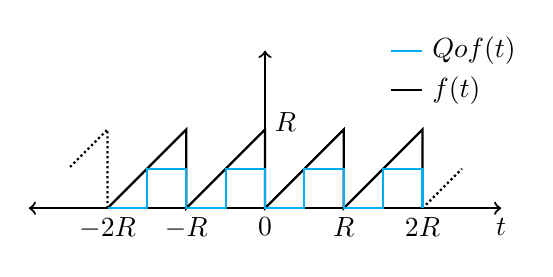
\begin{tikzpicture}
				\draw[<->,thick] (-3,0)--(3,0) node[anchor=north]{$t$};
				\draw (0,0) node[anchor=north]{$0$};
				\draw (0,1.1) node[anchor=west] {$R$};
				\draw (1,0) node[anchor=north]{$R$};
				\draw (2,0) node[anchor=north] {$2R$};
					\draw (-1,0) node[anchor=north]{$-R$};
				\draw (-2,0) node[anchor=north] {$-2R$};
				\draw[] (2,2) node[anchor=west] {{$Qof(t)$}};
				\draw[cyan,thick] (1.6,2) -- (2,2);
				%\draw [densely dotted,thick] (-2.5,1)--(3,1);
				\draw[->,thick] (0,0)--(0,2);
				\draw[] (2,1.5) node[anchor=west] {{$f(t)$}};
				\draw[thick] (1.6,1.5) -- (2,1.5);
				\draw[thick] (-2,0) --(-1,1)-| (-1,0) -- (0,1) -| (0,0) --(1,1)-| (1,0) -- (2,1) -| (2,0);
				\draw[densely dotted,thick] (2,0)--(2.5,0.5);
				\draw[densely dotted,thick] (-2,0)|-(-2,1) -- (-2.5,0.5);
				\draw[thick, cyan] (-2,0) -- ++(0.5,0)-| ++(0,0.5) -- ++(0.5,0) -| ++(0,-0.5) -- ++(0.5,0)-| ++(0,0.5) -- ++(0.5,0) -| ++(0,-0.5) -- ++(0.5,0)-| ++(0,0.5) -- ++(0.5,0) -| ++(0,-0.5) -- ++(0.5,0)-| ++(0,0.5) -- ++(0.5,0) -| ++(0,-0.5);
				\end{tikzpicture}}\\
			\multicolumn{3}{c}{(a)}\\
			\includegraphics[trim = 10mm 60mm 25mm 40mm,clip, width = 0.32\linewidth]{./orgimg.pdf}&
			\includegraphics[trim = 10mm 60mm 25mm 40mm,clip, width = 0.32\linewidth]{./modimg.pdf}&
			\includegraphics[trim = 10mm 60mm 25mm 40mm,clip,width = 0.32\linewidth]{./quantimg.pdf} \\
			(b) & (c) & (d)
		\end{tabular}
		\endgroup
	\end{center}
	\caption{\small{\emph{ (a) Modulo function, $f(t) = \mod(t,R)$ and quantized modulo function, $Qof(t)$; (b,c,d) Depiction of forward model. An input image (b) is transformed via a modulo function $f(t) = \mod(t,R)$, to (c). Such a ``modulo" image is further quantized to obtain (d).}}}
	\label{fig:func}
\end{figure}
%%%%%%%%%%%%%%%%%%%%%%%%%%%%%%%%%%%%%%%%%%%%%%%%%%

\subsection{Our contributions}

Clearly, the above estimation procedure is challenging due to the highly non-invertible nature of the observation model. In this paper, we design a systematic approach that takes some initial steps towards resolving this challenge. Our overarching assumption is that the measurement operations $A$ and $C$ are part of the design space. The core idea in our approach is that a very small, but carefully designed, non-adaptive set of measurements can support efficient estimation of the unknown signal.

Our approach follows stagewise. First, we consider the problem of inverting the quantization function, i.e., recovering $u$ from $y = Q(Cu)$. We demonstrate the existence of a linear operator $C$ (together with an efficient reconstruction algorithm) that supports such an inversion. Specifically, our operator $C$ obeys a particular block-diagonal form with weights chosen according to a harmonic progression; see Section~\ref{sec:Model} for details. We only consider 1-bit quantization functions, but similar ideas can presumably be extended for a higher number of quantization levels. In addition, our method supports the criterion of \emph{consistent reconstruction} as defined in \cite{jacques2011dequantizing}.

Next, we consider the problem of inverting the modulo operation, i.e., recovering $x$ from $u = f(Ax)$.  We propose an algorithm that builds upon the approach proposed in \cite{SoltaniHegde_ICASSP16}. In particular, we show that if the operator $A$ satisfies a certain \emph{factorization} $A = DB$, then $f$ can be stably inverted. To enable efficient inversion, the matrix $D$ must also be block-diagonal with weights chosen either randomly, or according to a geometric progression. In the former case, the reconstruction algorithm is an extension of the approach of~\cite{SoltaniHegde_ICASSP16}, while in the latter case the reconstruction follows the approach of~\cite{ICCP15_Zhao}.

The above two-stage procedure can be easily adapted to the case where we have some prior knowledge of the original signal $x$. This enables our approach to be used in conjunction with compressive imaging architectures. Common priors used in compressive imaging include \emph{sparsity} in some known orthonormal basis~\cite{foucart2013}. Note that our measurements are highly quantized and the total ``bit" complexity of our observations is far smaller than conventional techniques. Therefore, within our framework, one can choose to increase the number of quantizer measurements (rows of $C$) and/or modulo measurements (rows of $D$) in order to achieve better estimation performance.


Fig.~\ref{fig:demo} displays some representative results using our approach. We begin with a standard ``Peppers" image, compute a modulo transformation with three multiplexed measurements per pixel, and further modulate it with a sequence of three harmonic multipliers per measurement before passing it through a 1-bit quantizer. (In words, the overall ``oversampling factor" in our method is $9\times$.) The final binary measurements displayed in Fig.\ \ref{fig:demo}(a) are given as inputs to our reconstruction algorithm. The results from the first and second stages are displayed as images in Fig.\ \ref{fig:demo}(b). As is visually evident, our method is able to successfully reconstruct the image, as displayed in Fig.\ \ref{fig:demo}(c). 


\begin{figure}[t]
	\begin{center}
		\begingroup
		\setlength{\tabcolsep}{1pt} % Default value: 6pt
		\renewcommand{\arraystretch}{.1} % Default value: 1
		{\setlength{\tabcolsep}{1mm}
		\begin{tabular}{ccc|c|c}      %{c@{\hskip .1pt}c@{\hskip .1pt}c}
			\centering
			\includegraphics[trim = 30mm 60mm 40mm 65mm,clip, width = 0.15\linewidth]{./quant11.pdf}&
			\includegraphics[trim = 30mm 60mm 40mm 65mm,clip, width = 0.15\linewidth]{./quant12.pdf}&
			\includegraphics[trim = 30mm 60mm 40mm 65mm,clip, width = 0.15\linewidth]{./quant13.pdf}&
			\includegraphics[trim = 90mm 125mm 90mm 120mm,clip, width = 0.18\linewidth]{./mod11.pdf}&
				\multirow{3}{20mm}{\includegraphics[trim = 90mm 85mm 90mm 120mm,clip, width = \linewidth]{./dms_img.pdf}}\\
			\includegraphics[trim = 30mm 60mm 40mm 65mm,clip, width = 0.15\linewidth]{./quant21.pdf}& 
			\includegraphics[trim = 30mm 60mm 40mm 65mm,clip, width = 0.15\linewidth]{./quant22.pdf}&
			\includegraphics[trim = 30mm 60mm 40mm 65mm,clip, width = 0.15\linewidth]{./quant23.pdf}&
			\includegraphics[trim = 90mm 125mm 90mm 120mm,clip, width = 0.18\linewidth]{./mod21.pdf}&\\
			\includegraphics[trim = 30mm 50mm 40mm 65mm,clip, width = 0.15\linewidth]{./quant31.pdf}& 
			\includegraphics[trim = 30mm 50mm 40mm 65mm,clip, width = 0.15\linewidth]{./quant32.pdf}&
			\includegraphics[trim = 30mm 50mm 40mm 65mm,clip, width = 0.15\linewidth]{./quant33.pdf}& 
			\includegraphics[trim = 90mm 125mm 90mm 120mm,clip, width = 0.18\linewidth]{./mod31.pdf}&\\[1pt]
			\multicolumn{3}{c|}{(a)} &(b)&{\centering(c)}
		\end{tabular}}
		\endgroup
	\end{center}
	\caption{\small{\emph{Illustration of our approach. A given input image is modulated pixel-wise with three pre-chosen weights, passed through a modulo sensor, modulated again pixel-wise with three weights, and quantized to binary images. The resulting observations are shown in (a). The images in (b) and (c) represent the reconstruction of the modulo images, $\widehat{u}$ and the final image, $\widehat{x}$, respectively.}}}
	
	\label{fig:demo}
\end{figure}




%\section{Preliminaries}
%\label{sec:Preliminaries}
\section{The causal structure of doubly warped spacetimes}
\label{sec:chronologicalrelation}
%By a {\em \multiwarped spacetime} we understand a lorentzian manifold $(V,g)$ where
%\begin{equation}
%  \label{eq:1}
%  V:= \R \times M_{1} \times M_{2}\quad\hbox{and}\quad
%g=-dt^{2}+\alpha_{1}g_{1}+\alpha_{2}g_{2},
%\end{equation}
%being $(M_{i},g_{i})$ a Riemannian manifold for $i=1,2$.
%
%\smallskip

In this section we are going to characterize the chronological and causal relations in doubly warped spacetimes. First, recall that a {\em \multiwarped spacetime} is a multiwarped spacetime $(V,g)$ as in (\ref{eqqq}) with two fibers ($n=2$), that is,

\begin{equation}
  \label{eq:1-aux}
  V:= (a,b)\times M_{1} \times M_{2}\quad\hbox{and}\quad
g=-dt^{2}+\alpha_{1}g_{1}+\alpha_{2}g_{2}.
\end{equation}
%where $\alpha_i:\R\rightarrow (0,\infty)$ are positive smooth functions and $(M_{i},g_{i})$ are Riemannian manifolds for $i=1,2$.
%\begin{rem}\label{rem:infinito}
%Since the structures studied in this paper are invariant by conformal transformations, our analysis implicitly covers the case where the temporal interval $(a,b)$ is a proper subset of $\R$. In fact, otherwise, multiply the metric by an appropriate positive function in order to obtain another doubly warped spacetime in the same conformal class with $(a,b)=\R$.
%\end{rem}




%\begin{rem}\label{rem:infinito}
%  As we are going to be interested in causal structures, there is no loss of generality if we assume that $(a,b)\equiv \R$. In fact, given a metric as in \eqref{eq:1-aux}, let us consider $\beta:(a,b)\rightarrow (0,\infty)$ a function satisfying that:
%  \[
%\int_{c}^b \frac{1}{\sqrt{\beta(t)}}dt=\infty=\int_{a}^c\frac{1}{\sqrt{\beta(t)}}dt
%    \]
%    for some $c\in (a,b)$. Then,
%    \[
%      \begin{array}{rl}
%        {\mathfrak g}=& -dt^{2}+\alpha_{1}g_{1}+\alpha_{2}g_{2}\\ =& \beta \left(-\left(\frac{dt}{\sqrt{\beta}}\right)^2+ \frac{\alpha_1}{\beta}g_1+\frac{\alpha_2}{\beta}g_2\right)\\ = & \beta \left(-ds^2+\tilde{\alpha}_1g_1+\tilde{\alpha}_2g_2   \right) \\ =&\beta\, g,
%      \end{array}
%      \]
%      where $s\in \R$ as, from definition, $ds=dt/\sqrt{\beta}$. Moreover,
%
%      \[
%\int_{0}^{\infty} \frac{1}{\sqrt{\tilde{\alpha}_i(s)}}ds=\int_{c}^{a} \frac{1}{\sqrt{\alpha_i(t)}}dt, \qquad \int_{0}^{-\infty} \frac{1}{\sqrt{\tilde{\alpha}_i(s)}}ds=\int_{c}^{b} \frac{1}{\sqrt{\alpha_i(t)}}dt, \quad\hbox{ for $i=1,2$}.
%        \]
%        In conclusion, the metric $\mathfrak{g}$ is conformal to $g$, which is also a {\multiwarped} model where the time component belongs to the entire $\R$ and with warping functions preserving some integral condition. Therefore, unless stated otherwise (essentially, on the main results), we will always work considering {\multiwarped} models as follow:
%
%        \begin{equation}
%  \label{eq:1}
%  V:= \R \times M_{1} \times M_{2}\quad\hbox{and}\quad
%g=-dt^{2}+\alpha_{1}g_{1}+\alpha_{2}g_{2},
%\end{equation}
%
%\end{rem}
%}


Take $(t^e,x^e)\in V$ and $x^o\in M:=M_1\times M_2$. Denote by $C(x^o,x^e)$ the set of smooth curves in $M$ connecting $x^o$ with $x^e$. Given $c=(c_1,c_2)\in C(x^o,x^e)$, consider the unique future-directed lightlike curve $\rho:[s^o,s^e]\rightarrow V$ with $\rho(s)=(\tau_{c,t^e}(s),c(s))$ and $\tau_{c,t^e}(s^e)=t^e$. From the metric expression in (\ref{eq:1-aux}), the component $\tau_{c,t^e}(s)$ is determined by the Cauchy problem
\[
-\dot{\tau}_{c,t^e}^2+\alpha_1(\tau_{c,t^e})g_{1}(\dot{c}_1,\dot{c}_1)+\alpha_2(\tau_{c,t^e})g_{2}(\dot{c}_2,\dot{c}_2)=0,\qquad
    \tau_{c,t^e}(s^e)=t^e.
  \]
Consider the functional
\[\J_{x^o,(t^e,x^e)}: C(x^o,x^e) \rightarrow (a,b), \quad c \mapsto \tau_{c,t^e}(s^o).\]
A direct computation shows that $(t^o,x^o)\ll (t^e,x^e)$ if, and only if, there exists $c\in C(x^o,x^e)$ such that $t_o<\J_{x^o,(t^e,x^e)}(c)$. This property suggests the following definition for the {\em departure time function}:
\[
T:M\times \left((a,b)\times M\right)\rightarrow (a,b),\qquad T(x^{o},(t^{e},x^{e})):= {Sup}_{C}\J_{x^o,(t^e,x^e)}
\]
(compare with \cite[Section 2.9]{Perlick2004} and \cite[Section 4]{FS2}). By construction, this function characterizes the chronological relation in $(V,g)$, as follows:
\begin{equation}\label{e0}
(t^{o},x^{o}) \ll (t^{e},x^{e}) \;\; \Longleftrightarrow \;\;
t^{o}<T(x^{o},(t^{e},x^{e})).
\end{equation}
In particular, the chronological past of a given point $(t^e,x^e)$ is given by
\[
I^-\left((t^e,x^e) \right):=\{(t,x)\in (a,b)\times M: t<T(x,(t^e,x^e)) \}.
  \]
Given a future-directed timelike curve $\gamma(t)=(t,c(t))$, $t\in [\omega,\Omega)$, and a point $x\in M$, the transitivity of the chronological relaction $\ll$ ensures that the function $T(x,\gamma(t))$ is increasing on $t$. Hence, the chronological past of $\gamma$ can be written as
  \[
I^-(\gamma)=\{(s,x)\in (a,b)\times M: s<b_c(x):=lim_{t\rightarrow b}T(x,\gamma(t))\}.
    \]
%    \begin{rem}
%      The choice of $b_c$ to denote such a limit came motivated from the studies of the causal boundary for standard static  spacetimes, that can be considered as... In fact, as it can be deduced from CITA REQUERIDA, $T(x,(t^*,y))=t^*-d(x,y)$, and so, when...\footnote{Simplemente concretar lo anterior al caso estático estandar, a modo de ejemplo.}.
%    \end{rem}

Next, let us characterize the departure time function, and so, the chronological relations (recall (\ref{e0})), in terms of some integral conditions involving the warping functions $\alpha_i$ and the Riemannian distances $d_i$ associated to the fibers $(M_i,g_i)$, $i=1,2$.
To this aim, let us consider a future-directed causal curve $\gamma:  I \rightarrow V$,
$\gamma(s)=(t(s),c_{1}(s),c_{2}(s))$. From the metric expression in \eqref{eq:1-aux}:
\[
\frac{dt}{ds}(s)=\sqrt{-D+\frac{\mu_{1}}{\alpha_{1}\circ
t}+\frac{\mu_{2}}{\alpha_{2}\circ t}}(s),
\]
where $D:=g(d\gamma/ds,d\gamma/ds)\leq 0$ and
$\mu_{i}:=(\alpha_{i}\circ t)^2 g_{i}(dc_{i}/ds,dc_{i}/ds)$,
$i=1,2$. From the Inverse Function Theorem, previous formula translates into
\[
\frac{ds}{dt}(t)=\left(-(D\circ s)+\frac{\mu_{1}\circ s}{\alpha
_{1}}+\frac{\mu_{2}\circ s}{\alpha _{2}}\right)^{-1/2}.
\]
Therefore, if we denote $t^{o}=t(s^{o})$, $t^{e}=t(s^{e})$, we
deduce
\begin{equation}\label{eq:3}
\begin{array}{c}
\hbox{length}\left(c_{i}\mid_{[s^{o},s^{e}]}\right)=\int_{s^{o}}^{s^{e}}\sqrt{g_{i}(\dot
c_{i}, \dot c_{i})} ds=\int_{t^o}^{t^e}\sqrt{g_{i}(\dot c_{i}, \dot
c_{i})} \frac{ds}{dt} dt \qquad\qquad\qquad\quad \\
\;\quad\qquad\qquad\qquad =\int_{t^o}^{t^e}\frac{\sqrt{\mu_{i}\circ
s}}{\alpha_i(t)}\left(-(D\circ s)+\frac{\mu_{1}\circ
s}{\alpha_{1}(t)}+\frac{\mu_{2}\circ s}{\alpha_{2}(t)}\right)^{-1/2}dt
\qquad\hbox{for}\;\; i=1,2.
\end{array}
\end{equation}
In the particular case of being $\gamma$ a lightlike geodesic we have: (i) $D=0$ (lightlike character of $\gamma)$, (ii) $\mu_i\circ s$ are constants and (iii) $c_i$ are (pre-)geodesics on the corresponding Riemannian manifold $(M_i,g_i)$ (geodesic character of $\gamma$). So, from (\ref{eq:3}), one deduces (see \cite[Theorem 2]{FS} for details):
\begin{prop}\label{thm:characluzgeodesics}
  Let $(V,g)$ be a {\multiwarped} spacetime as in (\ref{eq:1-aux}) with (weakly) convex fibers (i.e., satisfying that any pair of points can be joined by some minimizing geodesic). Consider two distinct points $(t^o,x_1^o,x_2^o),(t^e,x_1^e,x_2^e)\in V$ with $t^o<t^e$. Then, the following statements are equivalent:
  \begin{itemize}
  \item[(a)] There exists a lightlike geodesic joining $(t^o,x_1^o,x_2^o)$ and $(t^e,x_1^e,x_2^e)$.
  \item[(b)] There exist $\mu_1,\mu_2 \ncambios{\geq}0$ with $\mu_1+\mu_2=1$ such that
    \[
\Integral{t^o}{t^{e}}{\mu_{i}}{i}{\mu_{k}}=d_{i}(x^{o}_{i},x^{e}_{i})\qquad\hbox{for}\;\;
i=1,2;
      \]

  \end{itemize}

\end{prop}


%This equality will be important in the forthcoming result, since it allows to explicitly compute the length of the projection of a causal curve over any of the Riemannian fibers.
%    \begin{lemma}
%\label{lightlikecurve}
%Let $(t^{o},x_1^o,x_2^o)$, $(t^e,x_1^{e},x_2^e)$  be two points of a \multiwarped spacetime $(V,g)$ as in \eqref{eq:1} such that $(x_1^o,x_2^o) \neq (x_1^{e},x_2^e)$. Assume the existence of positive values $\mu_{1},\mu_{2} \in\R$, with $\mu_{1}+\mu_{2}=1$, such that
%\begin{equation}\label{eq:2}
%\Integral{t^o}{t^e}{\mu_{i}}{i}{\mu_{k}}>d_{i}(x_{i}^o,x_{i}^{e}) \qquad\hbox{for}\;\;
%i=1,2.
%\end{equation}
%Then $(t^{o},x_1^o,x_2^o) \ll (t^{e},x_1^e,x_2^e)$, i.e., there exists a timelike future-directed curve between $(t^{o},x_1^o,x_2^o)$ and $(t^{e},x_1^e,x_2^e)$.
%\end{lemma}
%
%\begin{proof} For any $\epsilon>0$, let us denote
%  \[
%L^\epsilon_i:=\Integral{t^o+\epsilon}{t^e}{\mu_{i}}{i}{\mu_{k}}.
%    \]
% Take $\epsilon>0$ small enough so that the inequalities in \eqref{eq:2} still hold for $t_0+\epsilon$ instead of $t_0$. There exist curves $y_i:[s^0,s^e]\rightarrow M_i$, with $y_{i}(s^{o})=x_{i}^{o}$ and $y_{i}(s^{e})=x^{e}_{i}$, such that $length(y_{i})=L^\epsilon_{i}$, $i=1,2$. Next, consider the lightlike curve
%$\rho(s)=(\tau(s),\overline{y}_{1}(s),\overline{y}_{2}(s))$,
%with $\overline{y}_{i}$ reparametrizations of $y_{i}$,
%constructed by
%requiring
%\[
%\left\{\begin{array}{l}\dot{\tau}=\sqrt{\sum_{i=1}^{2}\frac{\mu_{i}}{\alpha_{i}\circ\tau}}
%\\ \tau(s^{e})=t^{e}
%\end{array}\right.,\qquad
%\left\{\begin{array}{l}g_{i}(\dot{\overline{y}}_{i},\dot{\overline{y}}_{i})=\frac{\mu_{i}}{(\alpha_{i}\circ
%\tau)^{2}} \\
%\overline{y}_{i}(s^{e})=x^{e}_{i}\end{array}\right.
%\qquad\hbox{for}\;\; i=1,2.
%\]
%Then, by applying \eqref{eq:3} to the lightlike curve $\rho$ (thus, $D=0$), we deduce
%\[
%\hbox{length}(\overline{y}_{i}\mid_{[\tau^{-1}(t^o+\epsilon),s^{e}]})=\Integral{t^o+\epsilon}{t^{e}}{\mu_{i}}{i}{\mu_{k}}
%%\int^{t^{e}}_{T'_{m}}\sqrt{\mu_{i}}\alpha_{i}^{-1}\left(\sum_{j=1}^{n}\frac{\mu_{j}}{\alpha_{j}}\right)^{-1/2}dt
%=L^\epsilon_{i}=\hbox{length}(y_{i}).
%\]
%Therefore, $\rho(s)$ is a lightlike curve joining $(t^o+\epsilon,x^{o})$ with
%$(t^{e},x^{e})$, and so, these points are causally related. Since $(t^0+\epsilon,x^0)\ll (t^0,x^0)$, it directly follows that $(t^0,x^0)\ll (t^{e},x^{e})$.
%\end{proof}
%
%In order to complete the characterization of the chronological relation, we will use the following characterization of the departure time function:
%
%%Assume just for a second that we have already obtained such an equivalence. Given $x^0,x^e\in M$ and $t^e$, the departure time function $T(x^0,(t^e,x^e))$ determines the exact point where the line $(t,x^0)$ with $t\in \R$ leaves the past of $(t^e,x^e)$. In particular, for all $t^0<T(x^0,(t^e,x^e))$ we can obtain $\mu_1,\mu_2$ so the inequalities on \eqref{eq:2} are satisfied. Therefore, at least intuitively, the departure time function should be in the edge of satisfying such inequalities, being expected that it satisfies a relation as in \eqref{eq:2} (substituing $t^0$ with $T(x^0,(t^e,x^e))$) but with equalities. The next result is a formalization of this intuitive idea:
%
%\begin{prop}
%\label{p0}
%Let $(V,g)$ be a \multiwarped spacetime and $(x^{o},(t^{e},x^{e}))\in M \times V$, with $x^{o}=(x_1^o,x_2^o)\neq (x_1^e,x_2^e)=x^{e}$. If $T=T(x^{o},(t^{e},x^{e}))>-\infty$ then $\varsigma=T$ is the unique real value satisfying
%\begin{equation}
%\label{e*}
%\Integral{\varsigma}{t^{e}}{\mu_{i}}{i}{\mu_{k}}=d_{i}(x^{o}_{i},x^{e}_{i}),\qquad
%i=1,2,
%\end{equation}
%for some (unique) constants $\mu_{1},\mu_{2} \geq 0$ with
%$\mu_{1}+\mu_{2}=1$.
%\end{prop}
%
%\begin{proof}
% First, let us show that if $\varsigma=T'$
%satisfies (\ref{e*}) then necessarily $T'\leq T$. To this aim,
%take any sequence $\epsilon_{m} \searrow 0$ and define for $i=1,2$
%\[
%L_{i,m}:=\Integral{T'_{m}}{t^{e}}{\mu_{i}}{i}{\mu_{k}}
%\qquad
%\hbox{with}\;\; T'_{m}:=T'-\epsilon_{m}.
%\]
%From the choice for $T'_m$, we have that $L_{i,m}>d_{i}(x_{i}^o,x_{i}^{e})$ for all $i$. So, Lemma \ref{lightlikecurve} ensures that
%$(T'_{m},x^o) \ll (t^e,x^e)$ for all $m$. Therefore, from the definition of $T(x^o,(t^e,x^e))$, $T'-\epsilon_{m}<T$ for all $m$, and then, $T' \leq T$.
%
%\medskip
%%From the hypothesis for $T'$, there exist curves $y_{i,m}(s)$ in
%%$M_{i}$ with lengths $L_{i,m}$ such that
%%$y_{i,m}(s^{o})=x_{i}^{o}$ and $y_{i,m}(s^{e})=x^{e}_{i}$.
%%Consider the lightlike curves
%%$\rho_{m}(s)=(\tau(s),\overline{y}_{1,m}(s),..., \overline{y}_{n,m}(s))$,
%%with $\overline{y}_{i,m}$ reparametrizations of $y_{i,m}$,
%%constructed by
%%requiring
%%\[
%%\left\{\begin{array}{l}\dot{\tau}=\sqrt{\sum_{i=1}^{2}\frac{\mu_{i}}{\alpha_{i}\circ\tau}}
%%\\ \tau(s^{e})=t^{e}
%%\end{array}\right.,\qquad
%%\left\{\begin{array}{l}g_{i}(\dot{\overline{y}}_{i,m},\dot{\overline{y}}_{i,m})=\frac{\mu_{i}}{(\alpha_{i}\circ
%%\tau)^{2}} \\
%%\overline{y}_{i,m}(s^{e})=x^{e}_{i}\end{array}\right.
%%\qquad\hbox{for}\;\; i=1,2.
%%\]
%%Then,
%%\[
%%\hbox{length}(\overline{y}_{i,m}\mid_{[\tau^{-1}(T'_{m}),s^{e}]})=\Integral{T'_{m}}{t^{e}}{\mu_{i}}{i}{\mu_{k}}
%%%\int^{t^{e}}_{T'_{m}}\sqrt{\mu_{i}}\alpha_{i}^{-1}\left(\sum_{j=1}^{n}\frac{\mu_{j}}{\alpha_{j}}\right)^{-1/2}dt
%%=L_{i,m}=\hbox{length}(y_{i,m}).
%%\]
%%Therefore, $\rho_{m}(s)$ joins $(T'_{m},x^{o})$ with
%%$(t^{e},x^{e})$, and so, the points $(T'_{m-1},x^{o})$,
%%$(t^{e},x^{e})$ are chronologically related for all $m$. According
%%to (\ref{e0}), this implies $T'<T+\epsilon_{m-1}$ for all $m$, and
%%thus, $T'\leq T$.
%
%Next, let us prove that some value $\varsigma=T'$
%verifying (\ref{e*}) always exists, and necessarily $T'\geq T$.
%From (\ref{e0}), $(t^{o},x^{o})\ll (t^{e},x^{e})$ for any
%$-\infty<t^{o}<T(x^{o},(t^{e},x^{e}))$. Let $\gamma:[t^0,t^e]\rightarrow V$,
%$\gamma(t)=(t,c_{1}(t), c_{2}(t))$, be a timelike curve such
%that $\gamma(t^{o})=(t^{o},x^{o})$ and $\gamma(t^{e})=(t^{e},x^{e})$.
%Consider real curves $\overline{c}_{i}$, $i=1,2$, such that
%\[
%\left\{\begin{array}{l} 0\leq\dot{\overline{c}}_{i}(t)\leq
%\sqrt{g_{i}(\dot{c}_{i}(s),\dot{c}_{i}(s))} \\
%\overline{c}_{i}(t^{o})=0 \\
%\overline{c}_{i}(t^{e})=d_{i}(x_{i}^{o},x_{i}^{e})
%\end{array}\right. \qquad\hbox{for}\;\; i=1,2.
%\]
%Then, $\overline{\gamma}(s)=(t,\overline{c}_{1}(t),\overline{c}_{2}(t))$
%becomes a future directed timelike curve in the globally hyperbolic \multiwarped
%spacetime
%$V'=(\R \times \R^{2},-dt^{2}+\alpha_{1}dx_{1}^{2}+\alpha_{2}dx_{2}^{2})$ joining $\overline{\gamma}(t^o)=\point{t^o}{0}{0}$ with $\overline{\gamma}(t^e)=\point{t^e}{d_{1}(x_{1}^o,x_{1}^{e})}{d_{2}(x_{2}^o,x_{2}^e)}$, i.e., \[\overline{\gamma}(t^o)=(t^o,0,0)\ll (t^e,d_{1}(x_{1}^o,x_{1}^{e}),d_{2}(x_{2}^o,x_{2}^{e})=\overline{\gamma}(t^e).\] Now consider $T'$ such that $(T',0,0)\leq \overline{\gamma}(t^e)$ but $(T',0,0)\not\ll \overline{\gamma}(t^e)$. From
%Avez and Seifert's result, there exists some lightlike geodesic in $\R\times \R^2$
%joining both points. Now, \cite[Theorem 2]{FS} (see also \cite[Lemma 3]{FS}) applied to the lightlike geodesic in $V'$ ensures that there exist unique positive constants $\mu_1,\mu_2$ with $\mu_1+\mu_2=1$ and such that
%
%\[
%\Integral{T'}{t^{e}}{\mu_{i}}{i}{\mu_{k}}=|d_{i}(x^{o}_{i},x^{e}_{i})-0|=d_{i}(x^{o}_{i},x^{e}_{i}) \qquad\hbox{for}\;\;
%i=1,2.
%  \]
%Finally, observe that $t^o<T'$ for all $t^o<T$, so in particular $T\leq T'$, which concludes the proof.
%
%% . \cambios{Denote by $\lambda(s)=(\tau(s),c_{1}(s),c_{2}(s))$ ($s \in [0,1]$) the
%% unique lightlike geodesic, and recall that a geodesic in a \multiwarped satisfies the following: (a) each $\mu_{i}=\alpha_{i}(\tau(s))^{2}g_{i}(c_{i}',c_{i}')$ is constant and (b) $c_{i}(s)$ is a pregeodesic in $(\mathbb{R},+dx_{i}^{2})$ for all $i$, see \cite{FS}[Eqns. (5), (6)]. Applying a change of variables in the following integral equalities by using the fact that $\frac{d\tau}{ds}=\sqrt{\sum_{i=1}^{2} \frac{\mu_{i}}{\alpha_{i} \circ \tau}}$ leads to:
%
%% \begin{equation}
%% \label{e7}
%% \hbox{length}(c_{i})=\int_{0}^{1}\sqrt{g_{i}(c_{i}',c_{i}')}dr=\Integral{T'}{t^{e}}{\mu_{i}}{i}{\mu_{k}}=d_{i}(x^{o}_{i},x^{e}_{i})\qquad\hbox{for
%% all}\;\; i
%% %\int^{t^{e}}_{T'}\sqrt{\mu_{i}}\alpha_{i}^{-1}\left(\sum_{j=1}^{n}\frac{\mu_{j}}{\alpha_{j}}\right)^{-1/2}dt=d_{i}(x^{o}_{i},x^{e}_{i})\qquad\hbox{for
%% %all}\;\; i
%% \end{equation}
%% }
%% \cambios{Note that $\mu_{1}$ and $\mu_{2}$ are unique for $T'$, in fact, if $\mu_{1}'$ and $\mu_{2}'$ are different to $\mu_{1}$ and $\mu_{2}$ then we have two possibilities: (1) $\mu_{1}'<\mu_{1}$ and $\mu_{2}<\mu_{2}'$ or (2) $\mu_{1}<\mu_{1}'$ and $\mu_{2}'<\mu_{2}$. Any of the previous cases imply that for some $i_{0} \in \{1,2\}$ the following strict inequality is obtained:
%% \[
%% \Integral{T'}{t^e}{\mu_{i_{0}}'}{i_{0}}{\mu_{k}'}>\Integral{T'}{t^e}{\mu_{i_{0}}}{i_{0}}{\mu_{k}}=d_{i_{0}}(x_{i_0}^o,x_{i_0}^e).
%% \]
%% So, $\mu_{1}$ and $\mu_{2}$ are the unique constants satisfying equation (\ref{e7}).
%% }
%%\footnote{For the uniqueness, and the forthcoming
%%property $(t^{o},x^{o})\not\ll (t^{e},x^{e})$, just apply [Subl.
%%3.4.2, PhD]: if $\mu_{i},\overline{\mu}_{i}\geq 0$,
%%$\mu_{1}+\cdots +\mu_{n}=1=\overline{\mu}_{1}+\cdots
%%+\overline{\mu}_{n}$ and $\overline{\mu}_{n}<\mu_{n}$ then there
%%exists some $i_{0}\in \{1,\ldots,n-1\}$ such that
%%$\overline{\mu}_{i_{0}}>\mu_{i_{0}}$ (and thus,
%%$\overline{\mu}_{n}/\overline{\mu}_{i_{0}}<\mu_{n}/\mu_{i_{0}}$)
%%and $\overline{\mu}_{j}/\overline{\mu}_{i_{0}}\leq
%%\mu_{j}/\mu_{i_{0}}$ $\forall j\neq n$.}
%% \cambios{Moreover, necessarily $T'\geq T$. In fact, if $T'<T$ then for any ${t^o}' \in (T',T)$ it cannot happen that
%% $({t^o}',x^{o}) \ll (t^{e},x^{e})$ since the same process to construct $T'$ will imply the existence of  $T''\in ({t^{o}}',T')$ such that $(T'',0)$ is causally but no
%% timelike related to $(t^{e},d_{1}(x_{1}^o,x_{1}),d_{2}(x_{2}^o,x_{2}^{e}))$ in the globally hyperbolic \multiwarped spacetime $(\R \times \R^{2},\hat{g})$, this will contradict the achronality of $\partial I_{\hat{g}}^{+}((t^{e},d_{1}(x_{1}^o,x_{1}),d_{2}(x_{2}^o,x_{2}^{e})))$ because $(T',0) \ll (T'',0)$ and both points live in the boundary. Therefore, for any ${t^{o}}' \in (T',T)$ we have that $({t^o}',x^{o}) \not \ll (t^{e},x^{e})$ and this is a contradiction to the condition over $T$ given in (\ref{e0}). Therefore, $T' \geq T$. The first part of the proof proves that $T \geq T'$ for any $T'$ satisfying equation (\ref{e*}), therefore $T$ is the only point satisfying equation (\ref{e*}) for unique constants $(\mu_{1},\mu_{2})$ with $\mu_{1}+\mu_{2}=1$. }
%\end{proof}
%
%\begin{rem}\label{rem:3}
% It is worth mentioning how in previous proof we have moved from the \multiwarped model $V$ to the globally hyperbolic \multiwarped model $V'$. This trick allow us to work in globally hyperbolic models which are complete, and so, where $\overline{I^\pm(p)}=J^\pm(p)$, being possible to obtain the integral condition more easily.\footnote{Jony: Este remark lo puse pensando en que este truco iba a volver a usarse más adelante, pero finalmente (al menos para el borde causal) no ha hecho falta. Mirar si vale la pena dejarlo.}
%\end{rem}
We are now in conditions to establish the characterization of the chronological relation.
\begin{prop}\label{c0}
Let $(V,g)$ be a \multiwarped spacetime as in (\ref{eq:1-aux}), and $(t^{o},x^{o}), (t^{e},x^{e})\in V$ with $x^{o}\neq
x^{e}$. The following conditions are equivalent:
\begin{itemize}

\item[(i)]  $(t^{o},x^{o})\ll (t^{e},x^{e})$; or, equivalently, $t^o<T(x^o,(t^e,x^e))$ (recall (\ref{e0}));
\item[(ii)] $T(x^o,(t^e,x^e))$ is the unique real value $T\in (a,b)$
with $t^{o}<T<t^{e}$ such that, for some (unique) positive constants $\mu_{1},\mu_2 \ncambios{\geq}
0$, with $\mu_{1}+\mu_{2}=1$, it satisfies
\begin{equation}\label{ee2}
\Integral{T}{t^{e}}{\mu_{i}}{i}{\mu_{k}}=d_{i}(x^{o}_{i},x^{e}_{i})\qquad\hbox{for}\;\;
i=1,2;
%\int_{T}^{t^{e}}\sqrt{\mu_{i}}\alpha_{i}^{-1}\left(\sum_{j=1}^{n}\frac{\mu_{j}}{\alpha_{j}}\right)^{-1/2}dt=d_{i}(x^{o}_{i},x^{e}_{i})\qquad\hbox{for}\;\;
%i=1,...,n;
\end{equation}

\item[(iii)] there exist strictly positive constants $\mu'_{1},\mu'_{2}> 0$, with $\mu'_1+\mu'_2=1$,
%(with
%$\mu'_{1}+\cdots +\mu'_{n}=1$)
such that
\begin{equation}\label{ee2''}
\Integral{t^{o}}{t^{e}}{\mu_{i}'}{i}{\mu_{k}'}>
d_{i}(x^{o}_{i},x^{e}_{i})\qquad\hbox{for $i=1,2$}.
%\int_{t^{o}}^{t^{e}}\sqrt{\mu'_{i}}\alpha_{i}^{-1}\left(\sum_{j=1}^{n}\frac{\mu'_{j}}{\alpha_{j}}\right)^{-1/2}dt\geq
%d_{i}(x^{o}_{i},x^{e}_{i})\qquad\hbox{for $i=1,...,n$},
\end{equation}
%with equality in the $i$-th inequality if and only if
%$\mu'_{i}=0$.
\end{itemize}
\end{prop}
\begin{proof}
%\footnote{He hecho cambios en esta prueba. Hay que chequear que todo es correcta.}
The implication $(ii)\Rightarrow (iii)$ is trivial unless some $\mu_i$ is equal to $0$. So, assume for instance that $\mu_1=0$ (and so, $\mu_2=1$). Then, \eqref{ee2} becomes
\[
\left\{
  \begin{array}{l}
    0=d_1(x_1^o,x_1^e)\\
    \\
    \displaystyle \int_{T}^{t^e}\frac{1}{\sqrt{\alpha_2(s)}}ds=d_2(x_2^o,x_2^e).
  \end{array}
\right.
  \]
  By continuity, we can modify slightly $\mu_1$, $\mu_2$, to obtain strictly positive $\mu'_1,\mu'_2$, with $\mu'_1+\mu'_2=1$, such that
 \[
    \left\{
      \begin{array}{l}\displaystyle\Integral{t^{o}}{t^{e}}{\mu_{1}'}{1}{\mu_{k}'}>0= d_1(x_1^o,x_1^e)\\
      \\
      \displaystyle\Integral{t^{o}}{t^{e}}{\mu_{2}'}{2}{\mu_{k}'}> d_2(x_2^o,x_2^e),
      \end{array}\right.
    \]
as desired.


For the implication $(iii) \Rightarrow (i)$, denote
  \[
L^\epsilon_i:=\Integral{t^o+\epsilon}{t^e}{\mu_{i}'}{i}{\mu_{k}'},\quad\hbox{for $\epsilon>0$.}
    \]
 Take $\epsilon>0$ small enough so that $t^o+\epsilon<t^e$ and the inequalities in \eqref{ee2''} still hold for $t^o+\epsilon$ instead of $t^o$. Since $L_i^{\epsilon}>d_i(x_i^o,x_i^e)$, there exist curves $y_i:[s^o,s^e]\rightarrow M_i$, with $y_{i}(s^{o})=x_{i}^{o}$ and $y_{i}(s^{e})=x^{e}_{i}$, such that $length(y_{i})=L^\epsilon_{i}$, $i=1,2$. Consider the lightlike curve
$\rho(s)=(\tau(s),\overline{y}_{1}(s),\overline{y}_{2}(s))$,
with $\overline{y}_{i}$ reparametrizations of $y_{i}$,
constructed by
requiring
\[
\left\{\begin{array}{l}\dot{\tau}=\sqrt{\sum_{i=1}^{2}\frac{\mu_{i}'}{\alpha_{i}\circ\tau}}
\\ \tau(s^{e})=t^{e}
\end{array}\right.,\qquad
\left\{\begin{array}{l}g_{i}(\dot{\overline{y}}_{i},\dot{\overline{y}}_{i})=\frac{\mu_{i}'}{(\alpha_{i}\circ
\tau)^{2}} \\
\overline{y}_{i}(s^{e})=x^{e}_{i}\end{array}\right.
\qquad\hbox{for}\;\; i=1,2.
\]
Then, by applying \eqref{eq:3} to the lightlike curve $\rho$ (in particular, $D=0$), we deduce
\[
\hbox{length}(\overline{y}_{i}\mid_{[\tau^{-1}(t^o+\epsilon),s^{e}]})=\Integral{t^o+\epsilon}{t^{e}}{\mu_{i}'}{i}{\mu_{k}'}
%\int^{t^{e}}_{T'_{m}}\sqrt{\mu_{i}}\alpha_{i}^{-1}\left(\sum_{j=1}^{n}\frac{\mu_{j}}{\alpha_{j}}\right)^{-1/2}dt
=L^\epsilon_{i}=\hbox{length}(y_{i}).
\]
Therefore, $\rho(s)$ is a lightlike curve joining $(t^o+\epsilon,x^{o})$ with
$(t^{e},x^{e})$, and so, these points are causally related. Since $(t^o,x^o)\ll (t^o+\epsilon,x^o)$, necessarily $(t^o,x^o)\ll (t^{e},x^{e})$.

Finally, for the implication $(i) \Rightarrow (ii)$, let us show first that if $T$
satisfies (\ref{ee2}) then $T\leq T(x^o,(t^e,x^e))$. So, assume that (\ref{ee2}) holds. %Up to a small modification of $\mu_i$, $i=1,2$, we can suppose that both coefficients are strictly positive.
Take any sequence $\epsilon_{m} \searrow 0$ and define
\[
L_{i,m}:=\Integral{T-\epsilon_m}{t^{e}}{\mu_{i}}{i}{\mu_{k}}\quad\hbox{i=1,2.}
\]
We have that $L_{i,m}>d_{i}(x_{i}^o,x_{i}^{e})$ for all $i$. The implication (iii)$\Rightarrow$(i), which has been proved before, ensures that
$(T-\epsilon_{m},x^o) \ll (t^e,x^e)$ for all $m$. Therefore, from the definition of $T(x^o,(t^e,x^e))$, $T-\epsilon_{m}<T(x^o,(t^e,x^e))$ for all $m$, and then, $T \leq T(x^o,(t^e,x^e))$.

%From the hypothesis for $T'$, there exist curves $y_{i,m}(s)$ in
%$M_{i}$ with lengths $L_{i,m}$ such that
%$y_{i,m}(s^{o})=x_{i}^{o}$ and $y_{i,m}(s^{e})=x^{e}_{i}$.
%Consider the lightlike curves
%$\rho_{m}(s)=(\tau(s),\overline{y}_{1,m}(s),..., \overline{y}_{n,m}(s))$,
%with $\overline{y}_{i,m}$ reparametrizations of $y_{i,m}$,
%constructed by
%requiring
%\[
%\left\{\begin{array}{l}\dot{\tau}=\sqrt{\sum_{i=1}^{2}\frac{\mu_{i}}{\alpha_{i}\circ\tau}}
%\\ \tau(s^{e})=t^{e}
%\end{array}\right.,\qquad
%\left\{\begin{array}{l}g_{i}(\dot{\overline{y}}_{i,m},\dot{\overline{y}}_{i,m})=\frac{\mu_{i}}{(\alpha_{i}\circ
%\tau)^{2}} \\
%\overline{y}_{i,m}(s^{e})=x^{e}_{i}\end{array}\right.
%\qquad\hbox{for}\;\; i=1,2.
%\]
%Then,
%\[
%\hbox{length}(\overline{y}_{i,m}\mid_{[\tau^{-1}(T'_{m}),s^{e}]})=\Integral{T'_{m}}{t^{e}}{\mu_{i}}{i}{\mu_{k}}
%%\int^{t^{e}}_{T'_{m}}\sqrt{\mu_{i}}\alpha_{i}^{-1}\left(\sum_{j=1}^{n}\frac{\mu_{j}}{\alpha_{j}}\right)^{-1/2}dt
%=L_{i,m}=\hbox{length}(y_{i,m}).
%\]
%Therefore, $\rho_{m}(s)$ joins $(T'_{m},x^{o})$ with
%$(t^{e},x^{e})$, and so, the points $(T'_{m-1},x^{o})$,
%$(t^{e},x^{e})$ are chronologically related for all $m$. According
%to (\ref{e0}), this implies $T'<T+\epsilon_{m-1}$ for all $m$, and
%thus, $T'\leq T$.

Next, it is sufficient to prove that some value $T$
verifying (\ref{ee2}) always exists, and necessarily $T\geq T(x^o,(t^e,x^e))$. Let $t'<T(x^o,(t^e,x^e))$, and thus, $(t',x^{o})\ll (t^{e},x^{e})$.
% We know that $(t^{o},x^{o})\ll (t^{e},x^{e})$.
Let $\gamma:[t',t^e]\rightarrow V$,
$\gamma(t)=(t,c_{1}(t), c_{2}(t))$, be a timelike curve such
that $\gamma(t')=(t',x^{o})$ and $\gamma(t^{e})=(t^{e},x^{e})$.
Consider real curves $\overline{c}_{i}$, $i=1,2$, such that
\[
\left\{\begin{array}{l} 0\leq\dot{\overline{c}}_{i}(t)\leq
\sqrt{g_{i}(\dot{c}_{i}(t),\dot{c}_{i}(t))} \\
\overline{c}_{i}(t')=0 \\
\overline{c}_{i}(t^{e})=d_{i}(x_{i}^{o},x_{i}^{e})
\end{array}\right. \qquad\hbox{for}\;\; i=1,2.
\]
Then, $\overline{\gamma}(t)=(t,\overline{c}_{1}(t),\overline{c}_{2}(t))$
becomes a future directed timelike curve in the globally hyperbolic \multiwarped
spacetime with convex fibers
$V'=(\ncambios{(a,b)} \times \R^{2},-dt^{2}+\alpha_{1}dx_{1}^{2}+\alpha_{2}dx_{2}^{2})$ joining $\overline{\gamma}(t')=\point{t'}{0}{0}$ with $\overline{\gamma}(t^e)=\point{t^e}{d_{1}(x_{1}^o,x_{1}^{e})}{d_{2}(x_{2}^o,x_{2}^e)}$, i.e., \[\overline{\gamma}(t')=(t',0,0)\ll (t^e,d_{1}(x_{1}^o,x_{1}^{e}),d_{2}(x_{2}^o,x_{2}^{e}))=\overline{\gamma}(t^e).\]
Consider $T>t'$ such that $(T,0,0)\leq \overline{\gamma}(t^e)$ but $(T,0,0)\not\ll \overline{\gamma}(t^e)$. From
Avez and Seifert's result, there exists some lightlike geodesic in $V'$
joining both points. Now, from Prop. \ref{thm:characluzgeodesics} applied to this lightlike geodesic, there exist unique positive constants $\ncambios{\mu_1,\mu_2 \geq}0$, with $\mu_1+\mu_2=1$, such that
\[
\Integral{T}{t^{e}}{\mu_{i}}{i}{\mu_{k}}=|d_{i}(x^{o}_{i},x^{e}_{i})-0|=d_{i}(x^{o}_{i},x^{e}_{i}) \qquad\hbox{for}\;\;
i=1,2.
  \]
Finally, since $t'<T$ for all $t'<T(x^o,(t^e,x^e))$, necessarily $T(x^o,(t^e,x^e))\leq T$, which concludes the proof.

\end{proof}

%\begin{rem}
%  Condition (iii) in previous theorem can be replaced by the following one:
%  {\em
%  \begin{itemize}
%  \item[(iii')] there exist constants $\mu'_{1},\mu'_{2}\geq 0$, with $\mu'_1+\mu'_2=1$,
%%(with
%%$\mu'_{1}+\cdots +\mu'_{n}=1$)
%such that
%\begin{equation}\label{e2''}
%\Integral{t^{0}}{t^{e}}{\mu_{i}'}{i}{\mu_{k}'}\geq
%d_{i}(x^{0}_{i},x^{e}_{i})\qquad\hbox{for $i=1,2$},
%%\int_{t^{o}}^{t^{e}}\sqrt{\mu'_{i}}\alpha_{i}^{-1}\left(\sum_{j=1}^{n}\frac{\mu'_{j}}{\alpha_{j}}\right)^{-1/2}dt\geq
%%d_{i}(x^{o}_{i},x^{e}_{i})\qquad\hbox{for $i=1,...,n$},
%\end{equation}
%with equality in the $i$-th inequality if and only if
%${\mu'}_{i}=0$.
%  \end{itemize}}
%  Now, the implication $(ii)\Rightarrow (iii')$ is straightforward. However, (iii) presents more clearly the open character of the chronological relation, which will be much more practical for the forthcoming sections.
%\end{rem}

Let us consider now the characterization of the causal relation (see \cite[Theorem 2(2)]{FS}).
 %In a first approach, one can think that it follows just by replacing the strict inequalities in condition (iii) of Thm. \ref{c0} by regular ones. However, this procedure forgets the necessity to include a convexity condition on each fiber, in order to ensure the existence of some lightlike geodesic connecting the two points.
 \begin{defi}
A Riemannian manifold $(N,h)$ is $L$-{\em convex} if any pair of points $p,q\in N$ with $d_h(p,q)<L$ can be joined by a minimizing geodesic.
\end{defi}
%Now, we can establish the announced characterization about the causal relation (see)
\begin{prop}
\label{p2'}
Let $(V,g)$ be a {\multiwarped} spacetime as in (\ref{eq:1-aux}) whose fibers $(M_i,g_i)$ are $L_i$-convex for $i=1,2$. Consider two points $\point{t^{o}}{x^o_{1}}{x^o_2}, \point{t^{e}}{x_1^{e}}{x_2^e} \in V$, with $t^o \leq t^e$, satisfying $d(x_i^o,x_i^e)<L_i$, $i=1,2$. Then, the following conditions are equivalent:
\begin{itemize}
\item[(i)] the points are causally related,
$\point{t^{o}}{x_1^{o}}{x_2^o} \leq \point{t^{e}}{x_1^{e}}{x_2^e}$;

\item[(ii)] there exists a causal geodesic joining $\point{t^{o}}{x_1^{o}}{x_2^o}$ with $\point{t^{e}}{x_1^{e}}{x_2^e}$;

\item[(iii)] there exist constants $\mu'_{1},\mu'_{2}\geq 0$, $\mu'_1+\mu'_2=1$,
%(with
%$\mu'_{1}+\cdots +\mu'_{n}=1$)
such that
\begin{equation}
\label{e2'''}
\Integral{t^{o}}{t^{e}}{\mu'_{i}}{i}{\mu'_{k}} \geq
d_{i}(x^{o}_{i},x^{e}_{i})\qquad\hbox{for}\;\;
i=1,2.
\end{equation}
\end{itemize}
Moreover, if the equalities hold in (\ref{e2'''}), then there is a lightlike and no timelike geodesic joining the points.
\end{prop}

%The proof of previous proposition, that can be found on \cite[Theorem 2]{FS}, relies on the following characterization of geodesics in doubly warped spacetimes (see \cite[(5) and (6)]{FS}): a curve $\gamma:I\rightarrow \R\times M_1\times M_2$ with $\gamma(t)=(\tau(t),c_1(t),c_2(t))$ is a geodesic if, and only if,
%
%\begin{equation}
%  \label{eq:31}
%  \begin{array}{rl}
%  \displaystyle \frac{d^2 \tau}{d t^2}=& \displaystyle -\left(\sum_{i=1}^2 \frac{\mu_i}{(\alpha_i\circ \tau)^{3/2}} \frac{d(\sqrt{\alpha_i})}{d\tau}\circ \tau \right)\\  & \\
%\displaystyle  \frac{D}{dt}\frac{d\,c_i }{dt}=& \displaystyle -\frac{2}{\sqrt{\alpha\circ \tau}} \frac{d(\sqrt{\alpha\circ \tau})}{dt} \frac{d\,c_i}{dt}, \quad \hbox{i=1,2}.
%  \end{array}
%\end{equation}\footnote{Nueva ecuacion sacada de otro artículo, verificar que no he metido la pata...}where $D/dt$ denotes the covariant derivative associated to each $g_i$ along $c_i$ and $\mu_i$ is the constant $(\alpha_i^2\circ \tau)g_i(d\,c_i/dt,d\,c_i/dt)$.


% \newpage


% \subsection{Chronological relation in multiwarped spacetimes}

% Let $(V,g)$ be a doublywarped spacetime, \cambios{in order to study
% the causal boundary of this kind of spacetimes we need to characterize the chronological relation $\ll$ in $(V,g)$.}
% For every piecewise smooth curve $c:[s^{o},s^{e}] \rightarrow M$
% with endpoints $c(s^{o})=x^{o}, c(s^{e}) =x^{e}$, consider the
% unique future-directed lightlike curve $\gamma(t)=(t,c(s(t))),
% t\in [T,t^{e}]$, being $s(t)$ and $T=T[c]$ determined by
% $g(\dot\gamma, \dot\gamma )\equiv 0, s(T)=s^{o},
% s(t^{e})=s^{e}$\footnote{If such a curve $\gamma$ does not exist
% (i.e. $s(t)>s^{o}$ for all $t<t^{e}$), just define
% $T=T[c]:=-\infty$.}. Let $C \equiv C(x^{o},x^{e})$ be the set of
% all such curves $c=c(s)$, and consider the functional
% $$\J: C \rightarrow \mathbb{R}, \quad c \mapsto T[c].$$
% Define a function $T: M \times (\R\times M) \rightarrow \R$ in the
% following way:
% $$(x^{o},(t^{e},x^{e})) \mapsto T(x^{o},(t^{e},x^{e})):= {Sup}_{C}\J.$$
% Then, one easily has:
% %\footnote{With this notation, the relation
% %between function $T$ and the {\em (time) arrival} map $\delta:
% %V\times M\rightarrow\R$ is $\delta((T,x^{o}),x^{e})=t^{e}-T$, with
% %$T=T(x^{o},(t^{e},x^{e}))$. (Apply the continuity of $\delta$.)}
% \begin{equation}\label{e0}
% (t^{o},x^{o}) \ll (t^{e},x^{e}) \;\; \Longleftrightarrow \;\;
% t^{o}<T(x^{o},(t^{e},x^{e})).
% \end{equation}
% %\footnote{When property (\ref{e0}) is applied to a causal curve
% %$\gamma(s)=(t(s),x(s))$, it translates into: $(t^{o},x^{o})\in
% %I^{-}[\gamma]\Leftrightarrow t^{o}<b_{\gamma}(x^{o})$, where
% %$b_{\gamma}(x^{o}):=\lim_{s}(t(s)-\delta(x^{o},(t(s),x(s))))$ can
% %be interpreted as the {\em Busemann function} associated to
% %$\gamma$.}
% %Notice that function $\delta$ is always finite and continuous, and
% %essentially the same function is obtained if past-directed causal
% %curves are taken.

% Let $\gamma:  I \rightarrow V$,
% $\gamma(s)=(t(s),x_{1}(s),x_{2}(s))$ be a future-directed causal
% curve. From the expression of $g$ in previous section, it is
% \[
% \frac{dt}{ds}(s)=\sqrt{-D+\frac{c_{1}}{\alpha_{1}\circ
% t}+\frac{c_{2}}{\alpha_{2}\circ t}}(s),
% \]
% where $D:=g(d\gamma/ds,d\gamma/ds)\leq 0$ and
% $c_{i}:=(\alpha_{i}^{2}\circ t)g_{i}(dx_{i}/ds,dx_{i}/ds)$,
% $i=1,2$. Then, from the Inverse Function Theorem:
% \[
% \frac{ds}{dt}(t)=\left(-(D\circ s)+\frac{c_{1}\circ s}{\alpha
% _{1}}+\frac{c_{2}\circ s}{\alpha _{2}}+...+\frac{c_{n}\circ s}{\alpha
% _{n}}\right)^{-1/2}(t)
% \]
% Therefore, if we denote $t^{o}=t(s^{o})$, $t^{e}=t(s^{e})$, we
% deduce
% \[
% \begin{array}{c}
% \hbox{length}\left(x_{i}\mid_{[s^{o},s^{e}]}\right)=\int_{s^{o}}^{s^{e}}\sqrt{g_{i}(\dot
% x_{i}, \dot x_{i})} ds=\int_{t^o}^{t^e}\sqrt{g_{i}(\dot x_{i}, \dot
% x_{i})} \frac{ds}{dt} dt \qquad\qquad\qquad\quad \\
% \;\quad\qquad\qquad\qquad =\int_{t^o}^{t^e}\frac{\sqrt{c_{i}\circ
% s}}{\alpha_i}\left(-(D\circ s)+\frac{c_{1}\circ
% s}{\alpha_{1}}+\frac{c_{2}\circ s}{\alpha_{2}}\right)^{-1/2}dt
% \qquad\hbox{for}\;\; i=1,2.
% \end{array}
% \]

% \ncambios{Last equality will be usefull in the Lemma below, because it allows to compute the length of the spatial components of a causal curve in terms of
% $\mu_{i}$'s and the warping functions.}

% \cambios{
% \begin{lemma}
% \label{lightlikecurve}
% Let $(t^{o},x^o)$ and $(t^e,x^{e})$ in $V$ \multiwarped spacetime with $x^o \neq x^{e}$. If there exists $(\mu_{1},\mu_{2}) \in (0,1)^{2}$ with $\mu_{1}+\mu_{2}=1$ and satisfying the following integral conditions:
% \[
% \Integral{t^o}{t^e}{\mu_{i}}{i}{\mu_{k}}>d_{i}(x_{i}^o,x_{i}^{e}) \qquad\hbox{for}\;\;
% i=1,2.
% \]
% Then $(t^{o},x^o) \ll (t^e,x^{e})$, i.e., there exists a timelike future directed curve between $(t^{o},x^o)$ and $(t^e,x^{e})$.
% \end{lemma}

% {\bf Proof:}

% The integral conditions and the continuity of the lower limit of the integral imply that there exists $\epsilon>0$ such that   $L_{i}^{\epsilon}:=\Integral{t^o+\epsilon}{t^e}{\mu_{i}}{i}{\mu_{k}}$ satisfies $L_{i}^{\epsilon}>d_{i}(x_{i}^o,x_{i}^{e})$ for all $i$, then, this last condition implies
% that there exists curves $y_{i}:[s^o,s^e] \rightarrow M_{i}$ such that $length(y_{i})=L_{i}^{\epsilon}$,
% $y_{i}(s^{o})=x_{i}^{o}$ and $y_{i}(s^{e})=x^{e}_{i}$. Consider the following lightlike curve
% $\rho(s)=(\tau(s),\overline{y}_{1}(s),\overline{y}_{2}(s))$,
% with $\overline{y}_{i}$ reparametrizations of $y_{i}$,
% constructed by
% requiring
% \[
% \left\{\begin{array}{l}\dot{\tau}=\sqrt{\sum_{i=1}^{2}\frac{\mu_{i}}{\alpha_{i}\circ\tau}}
% \\ \tau(s^{e})=t^{e}
% \end{array}\right.,\qquad
% \left\{\begin{array}{l}g_{i}(\dot{\overline{y}}_{i},\dot{\overline{y}}_{i})=\frac{\mu_{i}}{(\alpha_{i}\circ
% \tau)^{2}} \\
% \overline{y}_{i}(s^{e})=x^{e}_{i}\end{array}\right.
% \qquad\hbox{for}\;\; i=1,2.
% \]
% Then,
% \[
% \hbox{length}(\overline{y}_{i}\mid_{[\tau^{-1}(t^o+\epsilon),s^{e}]})=\Integral{t^o+\epsilon}{t^{e}}{\mu_{i}}{i}{\mu_{k}}
% %\int^{t^{e}}_{T'_{m}}\sqrt{\mu_{i}}\alpha_{i}^{-1}\left(\sum_{j=1}^{n}\frac{\mu_{j}}{\alpha_{j}}\right)^{-1/2}dt
% =L_{i}^{\epsilon}=\hbox{length}(y_{i}).
% \]
% Therefore, $\rho(s)$ joins $(t^o+\epsilon,x^{o})$ with
% $(t^{e},x^{e})$, and so, the points $(t^{o},x^{o})$,
% $(t^{e},x^{e})$ are chronologically related since $(t^o,x^o) \ll (t^{o}+\epsilon,x^o) \leq (t^e,x^e)$.
% \begin{flushright}
% $\spadesuit$
% \end{flushright}
% \medskip

% \ncambios{Luis:
% Previous lemma can be extended to the following cases: (1) some $\mu_{i}$ is equal to zero or (2) some $x_{i}^{o}$ is equal to $x_{i}^{e}$. The construction of the causal curve can be carried out as in the proof of previous lemma with the difference that we will be working in the Riemannian manifold $(M_{j},g_{j})$ in which $\mu_{j}\neq 0$ or $x_{j}^{o} \neq x_{j}^{e}$ and we will obtain a curve with $i$ component equal to a constant point $x_{i}^{o}=x_{i}^{e}$.
% }
% \medskip

% Next result will give an analytic characterization of $T(x^{o},(t^{e},x^e))$ defined before:
% }

% \begin{prop}
% \label{p0}
% Let $(V,g)$ be a \multiwarped spacetime and $(x^{o},(t^{e},x^{e}))\in M \times V$, with $x^{o}\neq x^{e}$. If $T=T(x^{o},(t^{e},x^{e}))>-\infty$ then $\varsigma=T$ is the unique value satisfying
% \begin{equation}
% \label{e*}
% \Integral{\varsigma}{t^{e}}{\mu_{i}}{i}{\mu_{k}}=d_{i}(x^{o}_{i},x^{e}_{i}) \qquad\hbox{for}\;\;
% i=1,2
% \end{equation}
% for some (unique) constants $\mu_{1},\mu_{2} \geq 0$ with
% $\mu_{1}+\mu_{2}=1$.
% \end{prop}
% {\it Proof.} First, we are going to show that if $\varsigma=T'$
% satisfies (\ref{e*}), then necessarily $T'\leq T$. To this aim,
% take any sequence $\epsilon_{m} \searrow 0$ and define
% \[
% L_{i,m}:=\Integral{T'_{m}}{t^{e}}{\mu_{i}}{i}{\mu_{k}}
% \qquad
% \hbox{for}\;\; i=1,2 \quad\hbox{with}\;\; T'_{m}:=T'-\epsilon_{m}.
% \]
% \cambios{From the hypothesis for $T'$, we have that $L_{i,m}>d_{i}(x_{i}^o,x_{i}^{e})$ for all $i$, then Lemma \ref{lightlikecurve} implies that
% $(T'_{m},x^o) \ll (t^e,x^e)$ for all $m$, then, $T'-\epsilon_{m}<T$ for all $m$ and therefore $T' \leq T$.
% }
% \medskip
% %From the hypothesis for $T'$, there exist curves $y_{i,m}(s)$ in
% %$M_{i}$ with lengths $L_{i,m}$ such that
% %$y_{i,m}(s^{o})=x_{i}^{o}$ and $y_{i,m}(s^{e})=x^{e}_{i}$.
% %Consider the lightlike curves
% %$\rho_{m}(s)=(\tau(s),\overline{y}_{1,m}(s),..., \overline{y}_{n,m}(s))$,
% %with $\overline{y}_{i,m}$ reparametrizations of $y_{i,m}$,
% %constructed by
% %requiring
% %\[
% %\left\{\begin{array}{l}\dot{\tau}=\sqrt{\sum_{i=1}^{2}\frac{\mu_{i}}{\alpha_{i}\circ\tau}}
% %\\ \tau(s^{e})=t^{e}
% %\end{array}\right.,\qquad
% %\left\{\begin{array}{l}g_{i}(\dot{\overline{y}}_{i,m},\dot{\overline{y}}_{i,m})=\frac{\mu_{i}}{(\alpha_{i}\circ
% %\tau)^{2}} \\
% %\overline{y}_{i,m}(s^{e})=x^{e}_{i}\end{array}\right.
% %\qquad\hbox{for}\;\; i=1,2.
% %\]
% %Then,
% %\[
% %\hbox{length}(\overline{y}_{i,m}\mid_{[\tau^{-1}(T'_{m}),s^{e}]})=\Integral{T'_{m}}{t^{e}}{\mu_{i}}{i}{\mu_{k}}
% %%\int^{t^{e}}_{T'_{m}}\sqrt{\mu_{i}}\alpha_{i}^{-1}\left(\sum_{j=1}^{n}\frac{\mu_{j}}{\alpha_{j}}\right)^{-1/2}dt
% %=L_{i,m}=\hbox{length}(y_{i,m}).
% %\]
% %Therefore, $\rho_{m}(s)$ joins $(T'_{m},x^{o})$ with
% %$(t^{e},x^{e})$, and so, the points $(T'_{m-1},x^{o})$,
% %$(t^{e},x^{e})$ are chronologically related for all $m$. According
% %to (\ref{e0}), this implies $T'<T+\epsilon_{m-1}$ for all $m$, and
% %thus, $T'\leq T$.

% Next, we are going to prove that some value $\varsigma=T'$
% verifying (\ref{e*}) always exists, and necessarily $T'\geq T$.
% From (\ref{e0}), $(t^{o},x^{o})\ll (t^{e},x^{e})$ for any
% $-\infty<t^{o}<T(x^{o},(t^{e},x^{e}))$. Let
% $\rho(s)=(\tau(s),y_{1}(s), y_{2}(s))$ be a timelike curve such
% that $\rho(s^{o})=(t^{o},x^{o})$ and $\rho(s^{e})=(t^{e},x^{e})$.
% Consider $2$ curves $\overline{y}_{i}$ in $\R$ such that
% \[
% \left\{\begin{array}{l} 0\leq\dot{\overline{y}}_{i}(s)\leq
% \sqrt{g_{i}(\dot{y}_{i}(s),\dot{y}_{i}(s))} \\
% \overline{y}_{i}(s^{o})=0 \\
% \overline{y}_{i}(s^{e})=d_{i}(x_{i}^{o},x_{i}^{e})
% \end{array}\right. \qquad\hbox{for}\;\; i=1,2.
% \]
% Then, the curve
% $\overline{\rho}(s)=(\tau(s),\overline{y}_{1}(s),\overline{y}_{2}(s))$
% is a future directed timelike curve in the globally hyperbolic \multiwarped
% spacetime
% $(\R \times \R^{2},-dt^{2}+\alpha_{1}dx_{1}^{2}+\alpha_{2}dx_{2}^{2})$ joining $\overline{\rho}(s^o)=\point{t^o}{0}{0}$ with $\overline{\rho}(s^e)=\point{t^e}{d_{1}(x_{1}^o,x_{1}^{e})}{d_{2}(x_{2}^o,x_{2}^e)}$.
% Therefore, there exists some unique $T' \in (t^{o},t^{e})$ such that
% $(T',\overline{y}(s^{o}))\leq\overline{\rho}(s^{e})$ but
% $(T',\overline{y}(s^{o}))\not\ll \overline{\rho}(s^{e})$. From
% Avez and Seifert's result, there exists some lightlike geodesic
% joining $(T',\overline{y}(s^{o}))$ with $\overline{\rho}(s^{e})$. \cambios{Denote by $\lambda(s)=(\tau(s),c_{1}(s),c_{2}(s))$ ($s \in [0,1]$) the
% unique lightlike geodesic, and recall that a geodesic in a \multiwarped satisfies the following: (a) each $\mu_{i}=\alpha_{i}(\tau(s))^{2}g_{i}(c_{i}',c_{i}')$ is constant and (b) $c_{i}(s)$ is a pregeodesic in $(\mathbb{R},+dx_{i}^{2})$ for all $i$, see \cite{FS}[Eqns. (5), (6)]. Applying a change of variables in the following integral equalities by using the fact that $\frac{d\tau}{ds}=\sqrt{\sum_{i=1}^{2} \frac{\mu_{i}}{\alpha_{i} \circ \tau}}$ leads to:

% \begin{equation}
% \label{e7}
% \hbox{length}(c_{i})=\int_{0}^{1}\sqrt{g_{i}(c_{i}',c_{i}')}dr=\Integral{T'}{t^{e}}{\mu_{i}}{i}{\mu_{k}}=d_{i}(x^{o}_{i},x^{e}_{i})\qquad\hbox{for
% all}\;\; i
% %\int^{t^{e}}_{T'}\sqrt{\mu_{i}}\alpha_{i}^{-1}\left(\sum_{j=1}^{n}\frac{\mu_{j}}{\alpha_{j}}\right)^{-1/2}dt=d_{i}(x^{o}_{i},x^{e}_{i})\qquad\hbox{for
% %all}\;\; i
% \end{equation}
% }
% \cambios{Note that $\mu_{1}$ and $\mu_{2}$ are unique for $T'$, in fact, if $\mu_{1}'$ and $\mu_{2}'$ are different to $\mu_{1}$ and $\mu_{2}$ then we have two possibilities: (1) $\mu_{1}'<\mu_{1}$ and $\mu_{2}<\mu_{2}'$ or (2) $\mu_{1}<\mu_{1}'$ and $\mu_{2}'<\mu_{2}$. Any of the previous cases imply that for some $i_{0} \in \{1,2\}$ the following strict inequality is obtained:
% \[
% \Integral{T'}{t^e}{\mu_{i_{0}}'}{i_{0}}{\mu_{k}'}>\Integral{T'}{t^e}{\mu_{i_{0}}}{i_{0}}{\mu_{k}}=d_{i_{0}}(x_{i_0}^o,x_{i_0}^e).
% \]
% So, $\mu_{1}$ and $\mu_{2}$ are the unique constants satisfying equation (\ref{e7}).
% }
% %\footnote{For the uniqueness, and the forthcoming
% %property $(t^{o},x^{o})\not\ll (t^{e},x^{e})$, just apply [Subl.
% %3.4.2, PhD]: if $\mu_{i},\overline{\mu}_{i}\geq 0$,
% %$\mu_{1}+\cdots +\mu_{n}=1=\overline{\mu}_{1}+\cdots
% %+\overline{\mu}_{n}$ and $\overline{\mu}_{n}<\mu_{n}$ then there
% %exists some $i_{0}\in \{1,\ldots,n-1\}$ such that
% %$\overline{\mu}_{i_{0}}>\mu_{i_{0}}$ (and thus,
% %$\overline{\mu}_{n}/\overline{\mu}_{i_{0}}<\mu_{n}/\mu_{i_{0}}$)
% %and $\overline{\mu}_{j}/\overline{\mu}_{i_{0}}\leq
% %\mu_{j}/\mu_{i_{0}}$ $\forall j\neq n$.}
% \cambios{Moreover, necessarily $T'\geq T$. In fact, if $T'<T$ then for any ${t^o}' \in (T',T)$ it cannot happen that
% $({t^o}',x^{o}) \ll (t^{e},x^{e})$ since the same process to construct $T'$ will imply the existence of  $T''\in ({t^{o}}',T')$ such that $(T'',0)$ is causally but no
% timelike related to $(t^{e},d_{1}(x_{1}^o,x_{1}),d_{2}(x_{2}^o,x_{2}^{e}))$ in the globally hyperbolic \multiwarped spacetime $(\R \times \R^{2},\hat{g})$, this will contradict the achronality of $\partial I_{\hat{g}}^{+}((t^{e},d_{1}(x_{1}^o,x_{1}),d_{2}(x_{2}^o,x_{2}^{e})))$ because $(T',0) \ll (T'',0)$ and both points live in the boundary. Therefore, for any ${t^{o}}' \in (T',T)$ we have that $({t^o}',x^{o}) \not \ll (t^{e},x^{e})$ and this is a contradiction to the condition over $T$ given in (\ref{e0}). Therefore, $T' \geq T$. The first part of the proof proves that $T \geq T'$ for any $T'$ satisfying equation (\ref{e*}), therefore $T$ is the only point satisfying equation (\ref{e*}) for unique constants $(\mu_{1},\mu_{2})$ with $\mu_{1}+\mu_{2}=1$. }
% \begin{flushright}
% $\spadesuit$
% \end{flushright}



% %before implies $(t^{o},x^{o})\not\ll (t^{e},x^{e})$ for any
% %$T'<t^{o}<T$, which contradicts (\ref{e0})}. $\square$
% %Consider $n$ {\em complete} metrics
% %$\overline{g}_{1},\ldots,\overline{g}_{n}$ on
% %$M_{1},\ldots,M_{n}$, resp., such that $\overline{g}_{i}\geq
% %g_{i}$ and $\overline{g}_{i}$ agrees $g_{i}$ on the range of
% %$y_{i}$, $i=1,\ldots,n$. (As the range of $y_{i}$ is compact, the
% %metrics $\overline{g}_{i}$ can be constructed by a standard
% %partition of unity argument.) Now, the corresponding warped metric
% %$\overline{g}$ obtained by replacing $g_{i}$ by $\overline{g}_{i}$
% %in $g$ satisfy:
% %\begin{itemize}

% %\item[(a)] $\overline{g}$ is globally hyperbolic, because each
% %$\overline{g}_{i}$ is complete, \item[(b)] as
% %$\overline{g}_{i}=g_{i}$ on $y_{i}$, then $\gamma(s^{*})\in
% %\overline{I}^{+}((t^{o},x^{o}))$, where $\overline{I}^{+}(z)$
% %denotes the set of points which can be joined with $z$ by a
% %future-pointing $\overline{g}$-timelike curve, \item[(c)] by Avez
% %and Seifert's result, there exists a $\overline{g}^{1,2}$-timelike
% %geodesic joining the two points, \item[(d)] by previous
% %implication, there exist $\mu_{1},\ldots,\mu_{n}$ such that
% %inequalities (\ref{e2}) hold, putting in the right hand side of
% %each inequality the distance $\overline{d}_{i}$ associated to
% %$\overline{g}_{i}$, and \item[(e)] as $\overline{g}_{i}\geq
% %g_{i}$, the corresponding distances also satisfy
% %$\overline{d}_{i}\geq d_{i}$, and the desired inequalities are
% %obtained. % \begin{flushright}
% %$\spadesuit$
% %\end{flushright}
% %\end{itemize}
% \vspace{1mm}


% Now, we can establish the following useful characterizations of
% the chronologically relation in \multiwarped spacetimes:
% \begin{thm}\label{c0}
% Let $(V,g)$ be a multiwarped spacetime and $(t^{o},x^{o}), (t^{e},x^{e})\in V$ with $x^{o}\neq
% x^{e}$. The following conditions are equivalent\footnote{Habra que comentar en algun sitio que los resultados
% anteriores, y, por tanto, los siguientes, son trivialmente
% extensibles al caso $(t^o,x^o)\in \R\times \overline{M}_C$. de
% hecho, esto ya se esta usando en la Proposicion \ref{r} (2).}:
% \begin{itemize}

% \item[(i)] The points are chronologically related,
% $(t^{o},x^{o})\ll (t^{e},x^{e})$;
% \item[(ii)] there exist some
% unique $t^{o}<T<t^{e}$ and (unique) constants $\mu_{1},\mu_2 \geq
% 0$ with $\mu_{1}+\mu_{2}=1$ such that
% \begin{equation}\label{e2}
% \Integral{T}{t^{e}}{\mu_{i}}{i}{\mu_{k}}=d_{i}(x^{o}_{i},x^{e}_{i})\qquad\hbox{for}\;\;
% i=1,...,n;
% %\int_{T}^{t^{e}}\sqrt{\mu_{i}}\alpha_{i}^{-1}\left(\sum_{j=1}^{n}\frac{\mu_{j}}{\alpha_{j}}\right)^{-1/2}dt=d_{i}(x^{o}_{i},x^{e}_{i})\qquad\hbox{for}\;\;
% %i=1,...,n;
% \end{equation}

% \item[(iii)] there exist constants $\mu'_{1},\mu'_{2}\geq 0$
% %(with
% %$\mu'_{1}+\cdots +\mu'_{n}=1$)
% such that
% \begin{equation}\label{e2''}
% \Integral{t^{o}}{t^{e}}{\mu_{i}'}{i}{\mu_{k}'}\geq
% d_{i}(x^{o}_{i},x^{e}_{i})\qquad\hbox{for $i=1,...,n$},
% %\int_{t^{o}}^{t^{e}}\sqrt{\mu'_{i}}\alpha_{i}^{-1}\left(\sum_{j=1}^{n}\frac{\mu'_{j}}{\alpha_{j}}\right)^{-1/2}dt\geq
% %d_{i}(x^{o}_{i},x^{e}_{i})\qquad\hbox{for $i=1,...,n$},
% \end{equation}
% with equality in the $i$-th inequality if and only if
% $\mu'_{i}=0$.
% \end{itemize}
% \end{thm}
% {\it Proof.} The equivalence $(i) \Leftrightarrow (ii)$ is direct
% from (\ref{e0}) and Prop. \ref{p0}. \cambios{The implication $(iii) \Rightarrow (i)$ is given by Lemma \ref{lightlikecurve}.
% Finally, the implication $(ii)\Rightarrow (iii)$ is
% trivial.
% \begin{flushright}
% $\spadesuit$
% \end{flushright}
% }
% \medskip

% \cambios{We can ensure that we can choose $\mu_{i}'$s non-zero in part $(iii)$ of previous result. This will be of help when we deal with the analytic characterization of
% the chronological relation.

% \begin{cor}
% \label{munonzero}
% Let $(V,g)$ be a multiwarped spacetime. If $(t^o,x^o)$ and $(t^{e},x^e)$ satisfies $x^o \neq x^e$ then the following statements are equivalent:
% \begin{enumerate}
% \item $(t^{o},x^o) \ll (t^e,x^e)$.
% \item There exist constants $\mu_{1},\mu_{2}>0$ with $\sum_{i=1}^{2} \mu_{i}=1$ and such that:
% \begin{equation}
% \label{e3}
% \Integral{t^o}{t^e}{\mu_{i}}{i}{\mu_{k}}>d_{i}(x^{o}_{i},x^{e}_{i})\qquad\hbox{for $i=1,2$}.
% %\int_{t^{o}}^{t^{e}}\sqrt{\mu_{i}}\alpha_{i}^{-1}\left(\sum_{j=1}^{n}\frac{\mu_{j}}{\alpha_{j}}\right)^{-1/2}dt >
% %d_{i}(x^{o}_{i},x^{e}_{i})\qquad\hbox{for $i=1,...,n$},
% \end{equation}
% \end{enumerate}
% \end{cor}

% {\bf Proof:}
% \smallskip
% Suppose that $(t^{o},x^o) \ll (t^e,x^e)$, then Prop. \ref{c0} (iii) implies the existence of $\mu'_{1},\mu'_{2}\geq 0$
% such that
% \begin{equation}
% \Integral{t^{o}}{t^{e}}{\mu_{i}'}{i}{\mu_{k}'}\geq
% d_{i}(x^{o}_{i},x^{e}_{i})\qquad\hbox{for $i=1,2$},
% %\int_{t^{o}}^{t^{e}}\sqrt{\mu'_{i}}\alpha_{i}^{-1}\left(\sum_{j=1}^{n}\frac{\mu'_{j}}{\alpha_{j}}\right)^{-1/2}dt\geq
% %d_{i}(x^{o}_{i},x^{e}_{i})\qquad\hbox{for $i=1,...,n$},
% \end{equation}
% with equality in the $i$-th inequality if and only if $\mu'_{i}=0$. Suppose, without lose of generality, that equality is achieved in the equation involving $\mu_{1}'$, then $\mu_{1}'=0$ and $\mu_{2}'=1$, since $x^o \neq x^e$ then $d_{2}(x_{2}^o,x_{2}^e)>0$ and $\int_{t^o}^{t^e}\frac{1}{\sqrt{\alpha_{2}}}ds>d_{2}(x_{2}^o,x_{2}^e)$. So,
% we can modify $(\mu_{1},\mu_{2})=(0,1)$ to obtain $(\mu_{1},\mu_{2})$ with $\mu_{1} \neq 0 \neq \mu_{2}$, $\mu_{1}<1$, $\mu_{2}>0$ and satisfying:
% \[
% \Integral{t^{o}}{t^{e}}{\mu_{i}}{i}{\mu_{k}} >
% d_{i}(x^{o}_{i},x^{e}_{i})\qquad\hbox{for $i=1,2$}.
% \]
% \medskip

% That $(2)$ implies $(1)$ is given by Lemma \ref{lightlikecurve}.
% \begin{flushright}
% $\spadesuit$
% \end{flushright}
% }

% Finally, and as useful result for the study of the causal hierarchy in the next subsection, we will give a characterization of the causal relation $\leq$ in
% \multiwarped spacetimes when each Riemannian manifold $(M_{i},g_{i})$ is $L_{i}$-weakly convex (see \cite[Thm. 2]{FS}.), where a Riemannian manifold is $L$-weakly convex if for any $x_{0}$ and $x_{1}$ such that $d(x_0,x_1) \leq L$ there exists a minimizing geodesic.
% %where $L_{i}$-weakly convex means that any pair of points $x^{o},x^{e} \in M_{i}$ with $d_{i}(x_{i}^{o},x_{i}^{e})<L_{i}$ can be joined by a minimizing geodesic.

% \begin{prop}
% \label{p2'}
% Let $V=\mathbb{R}\times_{\alpha_1}M_1 \times_{\alpha_2}M_2$ be a multiwarped spacetime whose fibers $(M_i,g_i)$ are $L_i$-weakly convex for $i=1,2$. Assume also that $\point{t^{o}}{x^o_{1}}{x^o_2}, \point{t^{e}}{x_1^{e}}{x_2^e} \in V$ and satisfying $d(x_i^o,x_i^e)<L_i$, $i=1,2$, with $t^o \leq t^e$. The following conditions are equivalent:
% \begin{itemize}
% \item[(i)] the points are causally related,
% $\point{t^{o}}{x_1^{o}}{x_2^o} \leq \point{t^{e}}{x_1^{e}}{x_2^e}$;

% \item[(ii)] there exists a causal geodesic joining $\point{t^{o}}{x_1^{o}}{x_2^o}$ with $\point{t^{e}}{x_1^{e}}{x_2^e}$;

% \item[(iii)] there exist constants $\mu'_{1},\ldots,\mu'_{n}\geq 0$
% %(with
% %$\mu'_{1}+\cdots +\mu'_{n}=1$)
% such that
% \begin{equation}
% \label{e2'''}
% \Integral{t^{o}}{t^{e}}{\mu'_{i}}{i}{\mu'_{k}} \geq
% d_{i}(x^{o}_{i},x^{e}_{i})\qquad\hbox{for $i=1,2$.}
% \end{equation}
% \end{itemize}
% Moreover if the equality holds in all equations, then there is a lightlike and no timelike geodesic joining the points.
% \end{prop}











%%% Local Variables:
%%% mode: latex
%%% TeX-master: "DoublyWarpedBoundary2017.tex"
%%% End:


%\section{Proof Sketch}
%\label{sec:proofsketch}
%\input{../ESN_RNN_normalizedseq/MainTheorem}
\section{Proof Sketch}
While the full proof is highly technical, in this section we will sketch the proof focusing on the conceptual aspects while minimizing the technical aspects to the essentials; full proofs are in the appendix. The high-level outline of our proof is as follows.
%\vspace{-3\topsep}
\begin{enumerate}[leftmargin=*, itemsep=0.1pt, topsep=0pt]
	\item \emph{Overparamtrization simplifies the neural network behavior.} The function $F_{\mathrm{rnn}}^{(L)}(\bx; \mathbf{W}+\mathbf{W}', \mathbf{A} + \mathbf{A}')$ computed by the RNN is a function of the parameters $\mathbf{W}', \mathbf{A}'$ as well as of the input $\overline{\mathbf{x}}$. It is a highly non-linear and non-convex function in both the parameters and in the input. The objective function inherits these properties and its direct analysis is difficult. However, it has been realized in the last few years---predominantly for the FFN setting---that when the network is overparametrized (i.e., as the number of neurons $m$ becomes large compared to other paramters of the problem such as the complexity of the concept class), the network behavior simplifies in a certain sense. The general idea carries over to RNNs as well:
	in \eqref{eqn:linear-approximation} below we write the first-order Taylor approximation of $F_{\mathrm{rnn}}^{(L)}(\bx; \mathbf{W}+\mathbf{W}', \mathbf{A} + \mathbf{A}')$
	at $\mathbf{W}$ and $\mathbf{A}$ as a linear function of  $\mathbf{W}'$ and $\mathbf{A}'$; it is still a non-linear function of the input sequence. As in \cite{allen2019can} we call this function \emph{pseudo-network}, though our notion is more general as we vary both the parameters $\mathbf{W}'$ and $\mathbf{A}'$. Pseudo-network is a good approximation of the target network as a function of $\overline{\mathbf{x}}$ for all $\overline{\mathbf{x}}$. \todo{This statement needs more work and also pointers to the formal statements.}
	\item \emph{Existence of a good RNN.} In order to show that the RNN training successfully learns, we first show that there are parameters values for RNN so that as a function of $\overline{\mathbf{x}}$ it is a good approximation of $F^\ast$. Instead of doing this directly, we show that the pseudo-network can approximate $F^\ast$; this suffices as we know that the RNN and the pseudo-network remain close. This is done by constructing paramters $\mathbf{W}^{\ast}$ and $\mathbf{A}^{\ast}$ so that the resulting pseudo-network approximates the target function in the concept class (Section~\ref{sec:fitting-target}) for all $\overline{\mathbf{x}}$. 
	\item \emph{Optimization.} SGD makes progress because the loss function is convex in terms of the pseudo-network which stays close to the RNN as a function of $\mathbf{x}$. Thus, SGD finds parameters with training loss close to that achieved by $\mathbf{W}^{\ast}, \mathbf{A}^{\ast}$.
	\item \emph{Generalization.} Apply a Rademacher complexity-based argument to show that SGD has low population loss.
\end{enumerate}
%\smallskip\smallskip
%\vspace{-2\topsep}
Step 2 is the main novel contribution of our paper and we will give more details of this step in the rest of this section.\footnote{The above outline is similar to prior work, e.g., \cite{allen2019can}. Details can be quite different though, e.g., they only train $\mathbf{W}$ and keep $\mathbf{A}$ fixed to its initial value. 
Their contribution was also mainly in Step 2 and the other steps were similar to prior work.} 
\subsection{Pseudo-network}\label{sec:pseudo-network}
%As mentioned, the most important step is to show the existence of a pseudo-network that approximates the target function for all inputs. 
We define the pseudo-network here. Suppose $\mathbf{W}, \mathbf{A}, \mathbf{B}$ are at random initialization.
 The linear term in the first-order Taylor approximation is given by the pseudo-network
%\todo{Give a reference in the AL paper for this. It's not explained what the function on the LHS is, nor are its arguments explained. Maybe remark on how this formula is obtained.}
\begin{align} 
	F^{(L)}(\bx; \mathbf{W}', \mathbf{A}') 
	&:= \sum_{i=1}^{L}  \mathbf{Back}_{i \rightarrow L} \mathbf{D}^{(i)} \left(\mathbf{W'} \mathbf{h}^{(i-1)} + \mathbf{A'} \mathbf{x}^{(i)}\right) \label{eqn:linear-approximation}\\&
	\approx F_{\mathrm{rnn}}^{(L)}(\bx; \mathbf{W}+\mathbf{W}', \mathbf{A}+\mathbf{A}') - F_{\mathrm{rnn}}^{(L)}(\bx; \mathbf{W}, \mathbf{A}) \tag{using Lemma~\ref{lemma:perturb_NTK_small_output}}.
\end{align}
 This function approximates the change in the output of the RNN, when $(\mathbf{W}, \mathbf{A})$ changes to $(\mathbf{W}+\mathbf{W}^{'}, \mathbf{A}+\mathbf{A}^{'})$. 
 The parameter $\lambda$, that we defined in the objective function, will be used to make the contribution of  $F_{\mathrm{rnn}}^{(L)}$ at initialization small thus making pseudo-network a good approximation of RNN. Hence, we can observe that the pseudo network is a good approximation of the RNN, provided the weights stay close to the initialization.
 
 To complete the above definition of pseudo-network we define the two new notations in the above formula. For each $\ell \in [L]$, define $\mathbf{D}^{(\ell)} \in \mathbb{R}^{m \times m}$ as a diagonal matrix, with diagonal entries %\todo{why do we need to use $d_{rr}^{(\ell)}$ why not $\mathbf{D}^{(\ell)}_{rr}$}
\begin{align}\label{eqn:diagonal_main}
	d_{rr}^{(\ell)} := \mathbb{I}[\mathbf{w}_r^{\top} \mathbf{h}^{(\ell - 1)} + \mathbf{a}_r^{\top} \mathbf{x}^{(\ell)} \ge 0], \quad \forall r \in [m]. 
\end{align}
In words, the diagonal of matrix $\mathbf{D}^{(\ell)}$ represents the activation pattern for the RNN cell at step $\ell$ at initialization.

Define $\mathbf{Back}_{i \to j} \in \mathbb{R}^{\dout  \times m}$ for each $1 \le i \le j \le L$ by
\begin{align*}
	\mathbf{Back}_{i \to j} := \mathbf{B} \mathbf{D}^{(j)} \mathbf{W} \ldots \mathbf{D}^{(i+1)} \mathbf{W}, 
\end{align*}
with $\mathbf{Back}_{i \to i} := \mathbf{B}$ for each $i \in [L]$. Matrices $\mathbf{Back}_{i \to j}$ in Eq. \eqref{eqn:linear-approximation} arise naturally in the 
computation of the first-order Taylor approximation (equivalently, gradients w.r.t. the parameters) using standard matrix calculus.% in terms of the parameters $\mathbf{W}, \mathbf{A}$ of the function $F_{\mathrm{rnn}}^{(\ell)}(\bx; \mathbf{W}, \mathbf{A})$. 
Very roughly, one can think of $\mathbf{Back}_{i \to j}$ as related to the backpropagation signal from the output at step $j$ to the parameters at step $i$. 




\subsection{Existence of good pseudo-network}\label{sec:fitting-target}
Our goal is to construct $\mathbf{W}^{\ast}$ and $\mathbf{A}^{\ast}$ such that for any true input sequence $\overline{\mathbf{x}} = (\overline{\mathbf{x}}^{(2)}, \ldots, \overline{\mathbf{x}}^{(L-1)})$, if we define the normalized sequence $\mathbf{x} = (\mathbf{x}^{(1)}, \ldots, \mathbf{x}^{(L)})$, then with high probability we have
\begin{align}\label{eq:simplifiedFstar}
    F^{(L)}(\bx; \mathbf{W}^{\ast}, \mathbf{A}^{\ast}) \approx   F^{\ast}(\overline{\mathbf{x}}).
\end{align}
%\sum_{r \in [p]} b^{\dagger}_{r, s} \Phi_{r, s} (\langle \mathbf{w}^{\dagger}_{r, s}, [\overline{\mathbf{x}}^{(2)}, \ldots, \overline{\mathbf{x}}^{(L-1)}]\rangle). 
%\end{align*}
\iffalse
The major challenge in constructing $\mathbf{W}^{\ast}$ and $\mathbf{A}^{\ast}$ is to use the information contained in $\mathbf{h}^{(\ell)}$ either explicitly in $\mathbf{h}^{(\ell)}$ or implicitly in $\mathbf{D}^{(i)}$ (recall \eqref{eqn:diagonal_main}). The construction of $\mathbf{W}^\ast$ 
in \cite{allen2019can} is not able to use this information and ignores it by treating it as noise (which is also non-trivial). Conceptually,
the idea underlying our construction is that $\mathbf{h}^{(\ell)}$ contains information about all the inputs $\bx^{(1)}, \ldots, \bx^{(\ell)}$ up until step $\ell$. Furthermore, this information can be recovered approximately by a linear transformation (Theorem~\ref{thm:Invertibility_ESN_outline}). Our construction sets $\mathbf{W}^{\ast} = \mathbf{0}$. This might suggest that we are  ignoring $\mathbf{h}^{(\ell)}$ as the RHS of \eqref{eqn:linear-approximation} becomes
\begin{align*} 
	F^{(L)}&(\bx; \mathbf{W}^\ast, \mathbf{A}^\ast) = \sum_{i=1}^{L}  \mathbf{Back}_{i \rightarrow L} \mathbf{D}^{(i)}  \mathbf{A'} \mathbf{x}^{(i)}.
\end{align*}
Moreover, this may appear to be a linear function in the $\mathbf{x}^{(i)}$. However, as just noted, $\mathbf{D}^{(i)}$ also implicitly has information about $\mathbf{h}^{(\ell)}$, and this is exploited in our construction of $\mathbf{A}^{\ast}$ to allow us to approximate general nonlinear functions of the $\mathbf{x}^{(i)}$.
\fi
To simplify the presentation, in this sketch we will assume that $p$, the number of neurons in the concept class, and the output dimension $\dout $ are both equal to $1$. 
Also, let the output weight $b^{\dagger}:=1$. 
These assumptions retain the main proof ideas while simplifying equations. %In the appendix full proofs are given.  
Overall, we assume that the target function $F^{\ast} : \Reals^{(L-2) \cdot (d-1)} \to \Reals$ on a given sequence is given by
\begin{align}\label{eqn:Fstar-Phi}
    F^{\ast}(\overline{\mathbf{x}}) = \Phi^{\ast}(\langle \mathbf{w}^{\dagger}, [\overline{\mathbf{x}}^{(2)}, \cdots, \overline{\mathbf{x}}^{(L-1)}]\rangle),
\end{align}
where $\Phi^{\ast}: \Reals \to \Reals$ is a smooth function and $\mathbf{w}^{\dagger} \in \mathbb{S}^{(L-2) \cdot (d-1) - 1}$. 

%In the following theorem, we will show that there exist some pseudo network that can approximately express this target function. 




First, we state Lemma 6.2 in \cite{allen2019learning}, which is useful for our construction of the matrices $\mathbf{W}^{\ast}$ and $\mathbf{A}^{\ast}$.
Consider a smooth function $\phi: [-1, 1] \to \Reals$. It can be approximated as a linear combination of step functions (derivatives of ReLU) for all $u \in (-1, 1)$, i.e., there exists a ``weight function'' $H: \Reals^2 \to \Reals$ such that
$	 \phi\left(u\right) \approx \mathbb{E}_{\alpha_1, \beta_1, b_0} [{H\left(\alpha_{1}, b_0\right)} \, \mathbb{I}_{\alpha_{1} u + \beta_{1} \sqrt{1 - u^{2}} + b_0   \geq 0}]$
where $\alpha_1, \beta_1 \sim \mathcal{N}\left(0, 1\right) \text{ and } b_0 \sim \mathcal{N}\left(0, 1\right)$ are independent random variables (we omitted some technical details).

The above statement can be straightforwardly extended to the following slightly more general version: 
\begin{lemma}\label{lemma:Expressfunction_fNN}
    For every smooth function $\phi$, any $\overline{\mathbf{w}} \in \mathbb{S}^{d-1}$, and any $\varepsilon \in \left(0, \frac{1}{\mathfrak{C}_{s}\left(\phi, 1 \right)}\right)$ there exists a $H:\mathbb{R}^2 \to \left(- 
	\mathfrak{C}_\varepsilon\left(\phi,  1\right),  \mathfrak{C}_\varepsilon\left(\phi,  1\right)\right)$, which is $ \mathfrak{C}_\varepsilon\left(\phi, 1\right)$-Lipschitz continuous and for all $\mathbf{u} \in  \mathbb{S}^{d-1}$, we have
	$$
	\begin{array}{l}
		\Big|\phi(\overline{\mathbf{w}}^{\top} \mathbf{u}) - \mathbb{E}_{\mathbf{w} \sim \mathcal{N}(\mathbf{0}, \mathbf{I}), b_0 \sim \mathcal{N}(0, 1)} [{H(\mathbf{w}^{\top} \overline{\mathbf{w}}, b_0)} \,\mathbb{I}_{\mathbf{w}^{\top} \mathbf{u} + b_0 \geq 0} ]  \Big| \leq \varepsilon.
	\end{array}
	$$
	%\end{corollary}
\end{lemma} 
Very informally, this lemma states that the activation pattern of a one-layer $\relu$ network (given by $\mathbb{I}_{\mathbf{w}^{\top} \mathbf{u} \geq 0}$) at initialization can be used to express a smooth function of the dot product of the input vector with a fixed vector. While the above statement involves an expectation, one can easily replace it by an empirical average with slight increase in error. 
This statement formed the basis for FFN and RNN results in \cite{allen2019learning, allen2019can}. 
%For completeness of the proof, we reproduce the argument here.
Can we use it for RNNs for our general concept class? An attempt to do so is the following lemma showing that the pseudo-network can express any smooth function of the hidden state $\mathbf{h}^{(L-1)}$ and $\mathbf{x}^{(L)}$. 

\begin{lemma}[Informal]\label{lemma:Expressfunction_RNN}
	%\begin{corollary}\label{Cor:Smooth_H}
	For a given smooth function $\phi$, a vector $\overline{\mathbf{w}} \in \mathbb{S}^{(m+d-1)}$, and any $\varepsilon \in \left(0, \frac{1}{\mathfrak{C}_{s}\left(\phi, 1 \right)}\right)$, there exist matrices $\mathbf{W}^{\ast}$ and $\mathbf{A}^{\ast}$ such that for every normalized input sequence $\bx = (\bx^{(1)}, \ldots, \bx^{(L)})$ formed from a sequence $\obx$, we have with high probability,
	\begin{align*}
	    \abs{F^{(L)}(\bx; \mathbf{W}^{\ast}, \mathbf{A}^{\ast}) - \phi({\langle  \overline{\mathbf{w}}, [\mathbf{h}^{(L-1)}, \bx^{(L)}_{:d-1}]\rangle})} \le \varepsilon,
	\end{align*}
	provided $m = \mathrm{poly}(\frac{1}{\varepsilon}, L, \mathfrak{C}_{\epsilon}(\phi, \mathcal{O}(1)))$. Vector $\bx^{(L)}_{:d-1}$ is 
	$\bx^{(L)}$ without the last coordinate, the bias term appended to each input.
	%\end{corollary}
\end{lemma} 
The reason $\mathbf{h}^{(L-1)}$ and $\mathbf{x}^{(L)}$ come up is because they serve as inputs to the RNN cell when processing the $L$-th input. The proof sketched below uses the fact that RNNs are one-layer FFNs unrolled over time. Hence, we could try to apply the result of Lemma~\ref{lemma:Expressfunction_fNN} to the RNN cell at step $L$. However, a difficulty arises in carrying out this plan because the contributions of previous times steps also come up (as seen in the equations below) and it can be difficult to disentangle the contribution of step $L$. This is addressed in the proof: 

\begin{prf}%[of Lemma~\ref{lemma:Expressfunction_RNN}]
    \input{ESN_RNN_normalizedseq/Proof_outline_2}
\end{prf}
More generally, with much more technical work, it might be possible to prove an extension of the above lemma asserting the existence of a pseudo-network approximating a sum of functions of type $\sum_{i \in [L]}\phi_i({\langle  \overline{\mathbf{w}}_i, [\mathbf{h}^{(i-1)}, \bx^{(i)}]\rangle})$. However, even so it is not at all clear what class of functions of $\overline{\mathbf{x}}$ this represents because of the presence of the hidden state vectors. 


Thus, the major challenge in constructing $\mathbf{W}^{\ast}$ and $\mathbf{A}^{\ast}$ to express the functions from the desired concept class is to use the information contained in $\mathbf{h}^{(\ell)}$. The construction of $\mathbf{W}^\ast$ in \cite{allen2019can} is not able to use this information and ignores it by treating it as noise (which is also non-trivial). The idea underlying our construction is that $\mathbf{h}^{(\ell)}$ in fact contains information about all the inputs $\bx^{(1)}, \ldots, \bx^{(\ell)}$ up until step $\ell$. Furthermore and crucially, this information can be recovered approximately by a linear transformation (Theorem~\ref{thm:Invertibility_ESN_outline} below). 
This enables us to show: \todo{Quantify }
\begin{theorem}[Existence of pseudo-network approximation for target function; abridged statement of Theorem~\ref{thm:existence_pseudo} in the appendix] \label{thm:existence_pseudo_outline}
	For every target function $F^{\ast}$ of the form Eq.~\eqref{eqn:Fstar-Phi}, there exist matrices $\mathbf{W}^{*}$ and $\mathbf{A}^{\ast}$ such that with probability at least $1-e^{-\Omega\left(\rho^{2}\right)}$ over $\mathbf{W}, \mathbf{A}, \mathbf{B}$, we have for every normalized input sequence $\mathbf{x} = (\mathbf{x}^{(1)}, \ldots, \mathbf{x}^{(L)})$ formed from a true sequence $\overline{\bx}$,  
	\begin{align*}
		\abs{F^{(L)}(\bx; \mathbf{W}^{\ast}, \mathbf{A}^{\ast}) - \Phi^{\ast} \left(\langle  \mathbf{w}^{\dagger}, [\overline{\mathbf{x}}^{(2)}, \ldots, \overline{\mathbf{x}}^{(L-2)}]\rangle\right)}  \le \varepsilon + \frac{1}{\mathrm{poly}(\rho)},   
	\end{align*}
	provided $m \ge \mathrm{poly}(\rho, L, \varepsilon^{-1}, \mathfrak{C}_{\varepsilon}(\Phi, \mathcal{O}(\varepsilon_x^{-1})))$ and $\epsilon_x \le \frac{1}{\mathrm{poly}(\rho)}$.
\end{theorem}

\begin{prf}[Proof sketch]
    \input{ESN_RNN_normalizedseq/Proof_outline_3}
\end{prf}

\emph{Re-randomization.} In the proof sketches of Lemmas~\ref{lemma:Expressfunction_RNN} and Theorem~\ref{thm:existence_pseudo_outline} above we swept a technical but critical consideration under the rug: the random variables $\{\mathbf{w}_r, \mathbf{a}_r\}_{r \in [m]}$, $\obW^{(L)}$, $\{\mathbf{Back}_{i \to L}\}_{i \in [L]}$ and $\{\mathbf{h}^{(i)}\}_{i \in [L]}$ are not independent. This invalidates application of standard concentration inequalities w.r.t. the randomness of $\mathbf{W}$ and $\mathbf{A}$---this application is required in the proofs. Here our new variation of the re-randomization technique from \cite{allen2019can} comes in handy. The basic idea is the following: whenever we want to apply concentration bounds w.r.t. the randomness of $\mathbf{W}$ and $\mathbf{A}$, we divide the set of rows into disjoint sets of equal sizes. For each set, we will re-randomize the rows of the matrix $[\mathbf{W}, \mathbf{A}]_r$, show that the matrices $\obW^{[L]}$, $\{\mathbf{Back}_{i \to L}\}_{i \in [L]}$ and $\{\mathbf{h}^{(i)}\}_{i \in [L]}$ don't change a lot and then apply concentration bounds w.r.t. the new weights in the set. Finally, we account for the error from each set.

%Hence, we need to follow the re-randomization technique again: divide the neurons into disjoint sets of equal size. For each set, we re-randomize the rows of the matrix $[\mathbf{W}, \mathbf{A}]_r$, show that $\obW^{[L]}$, $\{\mathbf{Back}_{i \to L}\}_{i \in [L]}$ and $\{\mathbf{h}^{(i)}\}_{i \in [L]}$ don't change a lot and then apply concentration w.r.t. $\{\mathbf{w}_r, \mathbf{a}_r\}_{r \in [m]}$. Finally, we accumulate the error from each set.
\subsection{The rest of the proof}
Having shown that there exists a pseudo-network approximation of the RNN that can also approximate the concept class,
%and overparametrized RNNs behave like linear networks close to initialization, 
we will complete the proof by showing that SGD can find matrices with performance similar to $\mathbf{W}^{\ast}$ and $\mathbf{A}^{\ast}$ on the population objective $\mathrm{Obj(\cdot)}$. Lemma~\ref{lem:trainloss}  shows that the training loss decreases with time. The basic idea is to use the fact that within small radius of perturbation, overparametrized RNNs behave as a linear network and hence the training can be analyzed via convex optimization. Then, we show using Lemma~\ref{lem:radcomp} that the Rademacher complexity for overparametrized RNNs is bounded. Again, the main idea here is that overparametrized  RNNs behave as pseudo-networks in our overparametrized regime and hence their Rademacher complexity can be approximated by the Rademacher complexity of pseudo-networks. Finally, using generalization bounds on the Rademacher complexity, we get the final population-level objective in  Theorem~\ref{thm:main_theorem}.



%Now, the optimization theorem in \cite{allen2019can} can be modified to show that SGD can find matrices with properties comparable to $\mathbf{W}^{\ast}$ and $\mathbf{A}^{\ast}$.

\subsection{Invertibility of RNNs at initialization}\label{sec:invertibility}
In this section, we describe how to get back $\bx^{(1)}, \ldots, \bx^{(L)}$ from the hidden state $\mathbf{h}^{(L)}$. %The following lemma states that any linear function can be represented by an infinitely sized neural network with activation function $\relu$ with the outer weights taking a very simple form:
%\begin{lemma}\label{lem:normal_linearestimate_outline}[Lemma~\ref{lem:normal_linearestimate} in the appendix]
%	For any $\bv \in \Reals^d$, the linear function taking $\bx$ to $\bv^\top \bx$ for $\bx \in \Reals^d$, can be represented as
%	\begin{equation}\label{eqn:single_layer_inversion_exact_outline}
%		\bv^\top \bx = \int_{\Reals^d} p(\bw) \, \sigma(\mathbf{w}^{\top} \bx ) \,\deriv \mu_d (\mathbf{w}),
%	\end{equation}
%	with 
%	$p\left(\mathbf{w}\right) \;=\;  2 \, \mathbf{w}^{\top} \mathbf{v}.$ 
%\end{lemma}
%The fact that $p(\mathbf{w})$ is a linear function is key to our application of this lemma.
%The proof follows from the second order moment of the normal distributed variables $\mathbf{w}$. 
%We can show using concentration properties of normal distributed variables that the above relation holds true for a highly overparametrized neural network, with a small approximation error of the order $\frac{1}{\sqrt{m}}$, i.e.
The following lemma states that any linear function can be represented by a one-hidden layer FFN with activation function $\relu$,with a small approximation error of the order $\frac{1}{\sqrt{m}}$:
\begin{lemma}\label{lem:normal_linearestimate_appr_outline} [a simpler continuous version can be found in Lemma~\ref{lem:normal_linearestimate} in the appendix]
	For any $\bv \in \Reals^d$, the linear function taking $\bx$ to $\bv^\top \bx$ for $\bx \in \Reals^d$, can be represented as
	\begin{equation}
		\abs{\bv^\top \bx -  \mathbf{p}^{\top} \sigma(\mathbf{T} \mathbf{x})} \le \frac{\norm{\bv} \cdot \norm{\bx}}{\sqrt{m}},
	\end{equation}
	with 
	$\mathbf{p} \;=\;  2 \, \mathbf{T} \mathbf{v},$ where $\mathbf{T} \in \mathbb{R}^{m \times d}$ is a matrix with elements i.i.d. sampled from $\mathcal{N}(0, 1)$. 
\end{lemma}
%The fact that $\mathbf{p}$   is key to our application of this lemma.
Using the above lemma,\footnote{This lemma is from a paper that will appear soon; apart from the above lemma, 
	this work is very different from the present paper. We have reproduced the proof in full in the appendix.} we will show that the hidden state $\mathbf{h}^{(L)}$ can be inverted using a matrix $\obW^{[L]}$ to get back the input sequence $\mathbf{x}^{(1)}, \ldots, \mathbf{x}^{(L)}$. 


%First, define an alternate fixed sequence as follows: $\bx_{(0)} := (\mathbf{x}^{(1)}_{(0)}, \ldots, \mathbf{x}^{(L)}_{(0)})$, where
%	\begin{align*}
%		\mathbf{x}^{(1)}_{(0)} = (\mathbf{0}^{d-1}, 1), \;\;\;
%		\mathbf{x}^{(\ell)}_{(0)} = (\mathbf{0}^{d-1}, \varepsilon_x), \quad \forall \ell \in [2, L-1], \;\;\;
%		\mathbf{x}^{(L)}_{(0)} = (\mathbf{0}^{d-1}, 1).
%	\end{align*}
%Denote the activation patterns for this fixed sequence as the diagonal matrices: $\{ \mathbf{D}_{(0)}^{(\ell)} \}_{\ell \in [L]}$. Then, we have

\todo{We need a bound on the norm of the $x$ or it should show up in the RHS}
\begin{theorem}\label{thm:Invertibility_ESN_outline}[informal version of Theorem~\ref{thm:Invertibility_ESN}]
	%Define $\obW^{[\ell]}$ inductively by $\obW^{[1]} = \mathbf{D}^{(1)}_{(0)} \mathbf{A} $ and $ \obW^{[\ell]}  = [\mathbf{D}^{(\ell)}_{(0)} \mathbf{W} \obW^{[\ell-1]}, \mathbf{D}_{(0)}^{(\ell)}\mathbf{A}]_r \quad \text{ for }\, 2 \le \ell \le L .$ 
	There exists a set of matrices $\{ \obW^{[\ell]} \}_{\ell \in [L]}$, which can possibly depend on $\mathbf{W}$ and $\mathbf{A}$, such that for any $\varepsilon_x < \frac{1}{L}$ and any given normalized sequence $\bx^{(1)}, \ldots, \bx^{(L)}$, 
	with probability at least $1 - e^{-\Omega(\rho^2)}$ we have
	$$
	\begin{array}{l}
		\norm[1]{[\bx^{(1)}, \ldots, \bx^{(L)}] - \obW^{[L]\top} \mathbf{h}^{(L)}}_\infty  \leq \mathrm{poly}(L, \rho, m^{-1}, \varepsilon_x).
	\end{array}
	$$
\end{theorem}
%\iffalse
%Informally, the proof follows from the simple observation that RNNs are one-layer FFNs unrolled over time. 
Very roughly, the above result is obtained by repeated application of Lemma~\ref{lem:normal_linearestimate_appr_outline} to go from $\mathbf{h}^{(\ell)}$ to $(\mathbf{h}^{(\ell-1)}, \mathbf{x}^{(\ell)})$ starting with $\ell = L$. This uses the fact that the RNN cell is a one-hidden layer neural network and hence Lemma~\ref{lem:normal_linearestimate_appr_outline} is applicable. Several difficulties need to be overcome to carry out this plan. One difficulty is that a naive application of Lemma~\ref{lem:normal_linearestimate_appr_outline}
results in exponential blowup of error with $L$. We defer the technical details of this resolution to the full proof in the appendix.
%We solve this issue using normalization. We observed that the factor $2$ in $\mathbf{p}$ from Lemma~\ref{lem:normal_linearestimate_appr_outline} can be removed by using the activation pattern of the input (given by $\sigma'(\mathbf{T} \bx)$) explicitly in $\mathbf{p}$.
%We estimate the activation pattern of each sequence, using the activation pattern of some fixed alternative sequence. That allows us to invert the RNN network, as if we were inverting a linear RNN. 
Secondly, we apply re-randomization to tackle the dependence between $\mathbf{W}$, $\mathbf{A}$, $\{\mathbf{h}^{(\ell)}\}_{\ell \in [L]}$ and $\{\obW^{[\ell]}\}_{\ell \in [L]}$.
%\fi
We performed few toy experiments on the ability of invertibility for  RNNs at initialization (Sec.~\ref{sec:expts}). We observed, as predicted by our theorem above, that the error involved in inversion decreases with the number of neurons and increases with the length of the sequence (Fig.~\ref{fig:RNN_inver}). 



%\begin{proof}[Proof of theorem~\ref{thm:Invertibility_ESN_outline}]
%    \input{../ESN_RNN_normalizedseq/Proof_outline_4}
%\end{proof}

%\subsection{Informal Proofs of the lemmas and theorems}

%\begin{proof}[Proof of lemma~\ref{lemma:Expressfunction_fNN}]
%    \input{../ESN_RNN_normalizedseq/Proof_outline_1}
%\end{proof}

%\begin{proof}[Proof of lemma~\ref{lemma:Expressfunction_RNN}]
%    \input{ESN_RNN_normalizedseq/Proof_outline_2}
%\end{proof}

%\begin{proof}[Proof of theorem~\ref{thm:existence_pseudo_outline}]
%    \input{ESN_RNN_normalizedseq/Proof_outline_3}
%\end{proof}



\section{On concept classes}

It is apparent that our concept class is very general as it allows arbitrary dependencies across tokens. To concretely illustrate the generality of our concept class, and to compare with previous work, we show that our result implies that  RNNs can recognize a simple formal language $D_{L_1}$. Here we are working in the discrete setting where each input token comes from $\{0, 1\}$ possibly represented as a vector when fed to the RNN. For a sequence $\mathbf{z} \in \{0, 1\}^L$, we define $D_{L_1}(\mathbf{z})$ to be $1$ if the number of $1$'s in $\mathbf{z}$ is exactly $1$ and define it to be $0$ otherwise. We can show that $D_{L_1}$ is not representable in the concept class of \cite{allen2019can} (see Theorem~\ref{thm:allencantdl1} in the appendix).  However, we can show that the language $D_{L_1}$ can be recognized with a one-layer FFN with one neuron and quadratic activation. The idea is that we can simply calculate the number of $1$'s in the input string, which is doable using a single neuron. This implies that our concept class can represent language $D_{L_1}$ with low complexity. More generally, we can show that our concept class can efficiently represent pattern matching problems, where strings belong to a language only if they contain given strings as substrings. In general, we can show that our concept class can express general regular languages. However, the complexity of the concept class may depend super-polynomially on the length of the input sequence, depending on the regular language (more discussion in sec.~\ref{sec:diff}). Some regular languages allow special treatment though. For example, consider the language $\mathsf{PARITY}$. $\mathsf{PARITY}$ is the language over alphabet $\{0, 1\}$ with a string $w = (w_1, \ldots, w_j) \in \mathsf{PARITY}$ iff
$w_1+\ldots +w_j = 1 \,\mathrm{mod}\, 2$, for $j \geq 1$. We can show in sec.~\ref{sec:diff} that $\mathsf{PARITY}$ is easily expressible by our concept class with small complexity. RNNs perform well on regular language recognition task in our experiments in Sec.~\ref{sec:expts}. Figuring out which regular languages can be efficiently expressed by our concept class remains an interesting open problem.


%which contains those strings that contain a particular substring. This is generally called the pattern matching problem. 

%a formal language $\mathsf{PARITY}$.  
%Here we are working in the discrete setting where each input token comes from $\{0, 1\}$ possibly represented as a vector when fed to the RNN. For a sequence $\mathbf{z} \in \{0, 1\}^L$, we define $\mathsf{PARITY}(\mathbf{z})$ to be $1$ if the number of $1$'s in $\mathbf{z}$ is odd and define it to be $0$ otherwise. 
%$\mathsf{PARITY}$ is known to be expressible by small one-hidden layer networks with $\relu$ activation; e.g. \cite[Lemma 5]{shalev2017failures}. The $\relu$ can be approximated by polynomials~\cite{lorentz}, implying that our concept class contains functions of small complexity that can approximate $\mathsf{PARITY}$. In Sec.~\ref{sec:diff} we show that  
%RNNs can recognize the language $\mathsf{PARITY}$---but 
%$\mathsf{PARITY}$ is not representable in the concept class of \cite{allen2019can}. 
%As mentioned before, RNNs are closely related to finite automata which accept regular languages.  $\mathsf{PARITY}$ is a regular language and the above result can be extended to many other regular languages. 








%\input{../ESN_RNN_normalizedseq/Lowerbound}

%\section{Experiments}
%\label{sec:experiments}
%\section{On Concept Classes}\label{sec:diff}
    The concept class in \cite{allen2019can} matched the output to a true label at each step using loss function $G$, i.e. $F^{\ast}$ belongs to $\mathbb{R}^{ L \times d} \to \Reals^{\dout}$, given by
    \begin{equation} \label{eqn:AL_concept_class}
    F^{\ast (j)}_s\left(\mathbf{x}\right) = \sum_{i : i < j} \sum_{r \in [p]} \phi_{i \to j, r, s} (\mathbf{w}_{i \to j, r, s}^T \mathbf{x}^{(i)}), 
    \end{equation}
    for all $j \in [2, L]$ and $s \in [\dout ]$. Here $\phi_{i \to j, r, s}: \Reals \to \Reals$ are smooth functions and $\mathbf{w}_{i \to j, r, s}$ unit vectors. We can rewrite \eqref{eqn:AL_concept_class} in a more compact vector form
    \begin{equation} \label{eqn:AL_concept_class_simplified}
        F^{\ast (j)}\left(\mathbf{x}\right) =  \sum_{i : i < j} \psi_{i \to j}(\mathbf{x}^{(i)}),
    \end{equation}
where $\psi_{i \to j}(\mathbf{x}^{(i)})$ is defined in the obvious way: it is the vector of inner sums in \eqref{eqn:AL_concept_class}.
 %for $s \in [\dout ]$. 
 From the previous equation it is clear that $F^{\ast (j)}(\mathbf{x}^{(i)})$ is a \emph{sum} of 
functions of individual tokens $\mathbf{x}^{(i)}$. This suggests that this concept class can represent only a limited set of concepts. A clean framework for illustrating these issues is afforded by the task of recognizing membership in a given formal language. Fix a finite alphabet $\Sigma$ with each letter also encoded by a vector so that it can be processed by RNNs. We say that the RNN recognizes a language $\Lambda$ over $\Sigma$ if after processing the sequences $(\bx^{(1)}, \ldots, \bx^{(j)})$ encoding a string $w = (w_1, \ldots, w_j) \in \Sigma^j$, the output $\mathbf{y}^{(j)}$ satisfies $\abs[0]{\mathbf{y}^{(j)}-1}<1/3$, if $w \in \Lambda$ and $\abs[0]{\mathbf{y}^{(j)}}<1/3$, otherwise. For simplicity, in the following, we will require the more stringent conditions $\mathbf{y}^{(j)}=1$ and  $\mathbf{y}^{(j)}=0$; these can be easily relaxed with some extra work. Since our output is binary, the output dimension $\dout $ is set to $1$; this is the setting in which our experiments are also done.

    Below, we give examples of some simple regular languages that the above concept class can't recognize but can be recognized by functions in our concept class with small complexity. 
  \iffalse
        \begin{theorem}
        $\mathsf{PARITY}$ cannot be represented by the concept class in \eqref{eqn:AL_concept_class}.
    \end{theorem}
\begin{proof} \emph{(sketch.)} For strings in $w \in \{0, 1\}^j$, we can rewrite \eqref{eqn:AL_concept_class_simplified} as 
        \begin{equation*}
        F^{\ast (j)}\left(\mathbf{x}\right)(w) =  \sum_{i : i < j} \alpha_i(w_i),
    \end{equation*}
where each $(\alpha_i(0), \alpha_i(1)) \in \Reals^2$ is any two-dimensional vector. Thus, $F^{\ast (j)}\left(\mathbf{x}\right)(w)$
can be written as a \emph{linear} function of $w$. It is easy to show and well-known that linear functions have correlation $0$ with $\mathsf{PARITY}$ \cite{odonnell} (this requires a standard linear change in parametrization to functions over $\{-1,1\}^j$ with output also in $\{-1,1\}$). 
\end{proof}
\fi

We first consider a simple regular language $L_1$ over the alphabet $\{0,1\}$ given by the regular expression $0^\ast 10^\ast$. In words, a string is in $L_1$ iff it contains a single $1$. This language can be thought of as modeling the occurrence of an event (a single blip) in a time series.

Consider the set $S$ of strings $\{0^q 00 0^{L-q-2}, 0^q 11 0^{L-q-2}, 0^q 01 0^{L-q-2}, 0^q 10 0^{L-q-2}\}$ where $0 \leq q \leq L-2$. 
Clearly, $0^q 00 0^{L-q-2} \notin L_1$ and $0^q 11 0^{L-q-2} \notin L_1$ whereas $0^q 01 0^{L-q-2} \in L_1$ and $0^q 10 0^{L-q-2} \in L_1$.
We choose uniform distribution on $S$ as the data distribution $D_{L_1}$. 
\begin{theorem}\label{thm:allencantdl1}
Any concept class of type \eqref{eqn:AL_concept_class} must err with probability at least $1/4$ on $D_{L_1}$.
\end{theorem}
\begin{proof}\emph{(sketch)} 
Fix a $q$. Let $w=0^q a b 0^{L-q-2}$ where $a, b \in \{0, 1\}$, we can rewrite \eqref{eqn:AL_concept_class_simplified} as 
\begin{align*}
    F^{\ast (L)}(w) &= 
    \sum_{i : i \leq q } \alpha_i(0) +  \alpha_{q+1}(a) + \alpha_{q+2}(b) + \sum_{i : q+3 \leq i \leq L } \alpha_i(0) \\
    &= A + \alpha_{q+1}(a) + \alpha_{q+2}(b),
\end{align*}
where each $(\alpha_i(0), \alpha_i(1)) \in \Reals^2$ is any two-dimensional vector.
Now, we must have $A + \alpha_{q+1}(1) + \alpha_{q+2}(0) = 1$ and $A + \alpha_{q+1}(0) + \alpha_{q+2}(1) = 1$. And also,
$A + \alpha_{q+1}(0) + \alpha_{q+2}(0) = 0$ and $A + \alpha_{q+1}(1) + \alpha_{q+2}(1) = 0$. Summing the first two equations gives
$2A +  \alpha_{q+1}(0)  + \alpha_{q+1}(1) + \alpha_{q+2}(0) + \alpha_{q+2}(1) = 2$ and summing the next two equations gives
$2A +  \alpha_{q+1}(0)  + \alpha_{q+1}(1) + \alpha_{q+2}(0) + \alpha_{q+2}(1) = 0$. Thus at least one of the four equations above must fail.
The concept class thus incurs an error with probability at least 1/4.
\end{proof}


We can show that our concept class (Eq.~\eqref{eq:concept_class}) can recognize the language $D_{L_1}$. Assume that we get an length-$L$ string as a length-$L$ input sequence $\bx$, with `$0$' represented by one-dimensional vector $0$ and `$1$' represented by one-dimensional vector $1$. E.g. `$0010$' will be represented as a sequence $0,0,1,0$. Then, one can count the number of $1$'s in the given input and claim that if the number of $1$'s is exactly $1$, the string belongs to the language $D_{L_1}$. The required condition can be checked using a single neuron with activation $\phi(x) = 2x - x^2$, which is a quadratic activation, and weight vector containing all ones ($\mathbf{1}$).  Hence, one can show that acceptance condition is satisfied iff $\phi(\langle\mathbf{1}, \bx\rangle + 1/2)$ is positive. Thus overall, we have shown that the language $D_{L_1}$ can be computed by a one-hidden layer neural network with a quadratic activation and $1$ neuron, implying that our concept class can approximate the language $D_{L_1}$.

\paragraph{Other pattern matching languages.} $D_{L_1}$ can be thought of as a very simple pattern matching problem.  In fact, we can show a more general class of languages that can be learned by our concept class efficiently. Consider the following language: a string (of length at most $L$) belongs to the language iff it contains a particular substring (of some constant length $k$). We will denote this substring by $\bar{s}$. Assume that we get an $L$-length string as $L$-dimensional input $\bx$, with `$0$' represented by a one-dimensional vector $-1$ and `$1$' represented by one-dimensional vector $1$. E.g. `$0010$' will be represented by the sequence $-1,-1,1,-1$. Let $\mathbf{v}_{\bar{s}}$ denote the vector representation of the sequence for the substring $\bar{s}$. Then, we can enumerate all the consecutive substrings in the input and check if the required substring occurs in at least one of them. Mathematically, this translates to creating a one layer neural network with $(L-k+1)$ neurons and activation function $\phi(t) = e^{ct}$, for some constant $c = \Omega(\log L)$. The $i$-th neuron will contain the weight vector $\mathbf{v}_i$, where the substring between position $i$ and $i+k-1$ contains $\mathbf{v}_{\bar{s}}$ and the rest of the positions contain $0$. One can check that if the input string contains the desired substring $\bar{s}$, then
$\sum_{i=1}^{L} \phi(\langle \mathbf{v}_i, \bx\rangle - k) \ge 1$, otherwise it is less than $\frac{1}{L}$. Thus, overall we have shown that the language can be recognized by a one-layer network with exponential activations. Since, we have discussed before that exponential activations have $O(1)$ complexity (see Def.~\ref{def:complexity}), we have shown that our concept class can efficiently solve the pattern matching problem.

We can generalize the above ideas to address some other related problems where we need to find multiple substrings, problems where we need to make sure that the number of times a particular substring occurs is at most a certain limit, etc.


\paragraph{General regular languages.} More generally, our concept class can express all regular languages. However, the complexity of the concept class can be super-polynomial in the sequence length $L$ depending on the regular language. Here is a sketch of a general construction.
As previously mentioned, RNNs with ReLU activations and finite precision are known to be equivalent to deterministic finite automata (DFA) and thus capture regular languages \cite{korsky2019computational}. 
    The ReLU can be approximated by polynomials \cite{lorentz} so that the resulting RNN still approximates the DFA up to some required length (the larger the length, the better the approximation needs to be---and the higher the degree of the approximating polynomial). In turn, such an RNN using polynomial activations can be easily represented by our concept class. The complexity (Def.~\ref{def:complexity}) of the concept class is small as polynomials have small complexity. We omit the routine but technical details of this construction. 
    
    Many regular languages allow special treatment though. For example, consider the language $\mathsf{PARITY}$. $\mathsf{PARITY}$ is the language over alphabet $\{0, 1\}$ with a string $w = (w_1, \ldots, w_j) \in \mathsf{PARITY}$ iff
$w_1+\ldots +w_j = 1 \,\mathrm{mod}\, 2$, for $j \geq 1$. We can show that $\mathsf{PARITY}$ is hard for the above concept class for the uniform distribution on $\{0,1\}^L$. A simple proof of this can be obtained via Boolean Fourier analysis (e.g., \cite{odonnell}) which we now sketch. In this setting, 
we note that $\mathsf{PARITY}$ of $L$ bits corresponds to a degree-$L$ polynomial $(2 w_1 -1 )(2w_2 -1)\ldots (2w_L-1)$; the output now takes values in $\{-1, 1\}$ instead of $\{0, 1\}$. On the other hand, the functions in \eqref{eqn:AL_concept_class} with $\dout=1$ correspond to linear functions of the form $\sum_i \alpha_i w_i + \beta_i$ for some constants $\alpha_i, \beta_i \in \Reals$ for all $i$. Using these facts, the correlation between the two can be easily shown to be $0$ via the Plancherel--Parseval theorem, which implies that all functions of type \eqref{eqn:AL_concept_class} make significant error on $\mathsf{PARITY}$. 

However, we can show that $\mathsf{PARITY}$ is easily expressible by our concept class with small complexity. Assume that we get an length-$L$ string as a length-$L$ input sequence $\bx$, with `$0$' represented by one-dimensional vector $0$ and `$1$' represented by one-dimensional vector $1$. E.g. `$0010$' will be represented as a sequence $0,0,1,0$. Then, one can count the number of $1$'s in the given input and claim that if the number of $1$'s is even, the string belongs to the language $\mathsf{PARITY}$. The required condition can be checked using a single neuron with activation $\phi(x) = \cos(\pi x)$ and weight vector containing all ones ($\mathbf{1}$). Hence, one can show that acceptance condition is satisfied iff $\phi( \langle\mathbf{1}, \bx\rangle - 1)$ is positive. Thus overall, we have shown that the language $\mathsf{PARITY}$ can be computed by a one-hidden layer neural network with a $\cos$ activation and $1$ neuron. Since, we have discussed before that $\cos$ activations have $O(1)$ complexity (see Def.~\ref{def:complexity}), we have shown that our concept class can efficiently recognize $\mathsf{PARITY}$.


%However, $\mathsf{PARITY}$ is known to be expressible by small one-hidden layer networks with $\relu$ activation; e.g. \cite[Lemma 5]{shalev2017failures}. The $\relu$ can be approximated by polynomials~\cite{lorentz}, implying that our concept class contains functions that can approximate $\mathsf{PARITY}$. However, we note here that to approximate $\relu$ within error $\varepsilon$ one needs a degree-$\mathrm{poly}(1/\varepsilon)$ polynomial and this also translates into high complexity of the concept class. %That implies, our concept class can have complexity exponential w.r.t. error $1/\epsilon$. 
%There might be a more efficient construcion of a concept class that learns the language $\mathsf{PARITY}$. This remains an interesting open problem.



We performed experiments on the ability of RNNs to learn various regular languages (see sec.~\ref{sec:expts} for details). In almost all of the regular languages that we tested on, RNNs can achieve near perfect test accuracies (table~\ref{table:regular}).

 \iffalse    
    \begin{theorem}
         Assume that the alphabet is $\{a, b\}$ and the sequences in $\mathcal{D}$ are generated from the language $a^{\ast}b^{\ast}a^{\ast}$ with positive label for strings of the form $a^{\ast} b a^{\ast}$ and a negative label for the rest. Also, assume that $\dout =2$ with an "accept" logit and a "reject" logit and the loss function $G$ is a classification loss (cross entropy, hinge loss, etc.) Then, any function in the above concept class will make an error on at least $\Omega(\frac{1}{L^2})$ fraction of the samples in $\mathcal{D}$.
         %The concept class can't capture the regular language $a^{*}ba^{*}$.
    \end{theorem}
    
    \begin{proof}
        We give a proof outline here. Consider the following strings: $a^{q-2}ba$, $a^{q-2}bb$, $a^{q-2}ab$ and $a^{q-2}aa$, for any $q \in [L]$. By the definition of the distribution $\mathcal{D}$, $a^{q-2}ba$ and $a^{q-2}ab$ have positive label, while $a^{q-2}aa$ and $a^{q-2}bb$ have negative label. Assume that a function $F^{\ast}$ classifies these strings correctly. We will assume that the vector representations of the letters $a$ and $b$ are given by $\bx(a)$ and $\bx(b)$ respectively. $F_{"accept"}^{(\ell)}$ denotes the "accept" logit score at cell $\ell$. Similarly define $F_{"reject"}^{(\ell)}$.   
        
        Given that the strings $a^{q-2}ab$ and $a^{q-2}aa$ must be accepted and rejected respectively, we can show that for any $t \ge q + 1$,
        \begin{align*}
        &\sum_{r \in [p]} ( \phi_{q \to t, r, "accept"} (\mathbf{w}_{q \to t, r, "accept"}^T \mathbf{x}(b)) \\& \quad\quad - \phi_{q \to t, r, "reject"} (\mathbf{w}_{q \to t, r, "reject"}^T \mathbf{x}(b))) \\& < \sum_{r \in [p]} ( \phi_{q \to t, r, "accept"} (\mathbf{w}_{q \to t, r, "accept"}^T \mathbf{x}(a)) \\& \quad\quad- \phi_{q \to t, r, "reject"} (\mathbf{w}_{q \to t, r, "reject"}^T \mathbf{x}(a) )).
        \end{align*}
        
        Similarly, given that the strings $a^{q-2}ba$ and $a^{q-2}bb$ must be accepted and rejected respectively, we can show that for any $t \ge q + 1$,       
        \begin{align*}
        &\sum_{r \in [p]}  ( \phi_{q \to t, r, "accept"} (\mathbf{w}_{q \to t, r, "accept"}^T \mathbf{x}(b)) \\& \quad\quad- \phi_{q \to t, r, "reject"} (\mathbf{w}_{q \to t, r, "reject"}^T \mathbf{x}(b)))  \\ & > \sum_{r \in [p]} ( \phi_{q \to t, r, "accept"} (\mathbf{w}_{q \to t, r, "accept"}^T \mathbf{x}(a)) \\& \quad\quad- \phi_{q \to t, r, "reject"} (\mathbf{w}_{q \to t, r, "reject"}^T \mathbf{x}(a))).
        \end{align*}
        However, both the equations contradict each other. Hence, any function $F^{\ast}$ must make a mistake at at least one of these strings. Counting the number of sets of such strings gives the final result.
    \end{proof}
\fi

\begin{comment}
\begin{figure}
\includegraphics[width=\linewidth]{figs/beyond_tss_lesion.pdf}
\caption[]{End-to-End runtime lesion study of the entire MNIST dataset and the FMA featurized music dataset. Each of DROP's contributions provides a runtime improvement.}
\label{fig:beyond_lesion}
\end{figure}
\end{comment}



\section{Conclusion}
\label{sec:conclusion}

Advanced data analytics techniques must scale to rising data volumes. 
DR techniques offer a powerful toolkit when processing these datasets, with PCA frequently outperforming popular techniques in exchange for high computational cost. 
In response, we propose DROP, a new dimensionality reduction optimizer. 
DROP combines progressive sampling, progress estimation, and online aggregation to identify high quality low dimensional bases via PCA without processing the entire dataset by balancing the runtime of downstream tasks and achieved dimensionality. 
Thus, DROP provides a first step in bridging the gap between quality and efficiency in end-to-end DR for downstream \red{analytics}. 

%We revisit canonical operators for time series dimensionality reduction and the measurement study of~\cite{keogh-study}, and show that PCA is more effective than popular alternatives in the data mining literature often by a margin of over $2\times$ on average on gold-standard time series benchmark data sets with respect to output data dimension. More surprisingly, we empirically demonstrate that a small number of samples are sufficient to accurately characterize directions of maximum variance and obtain a high-quality low-dimensional transformation.




% In the unusual situation where you want a paper to appear in the
% references without citing it in the main text, use \nocite
%\nocite{langley00}
%\newpage
\bibliographystyle{unsrt}
\bibliography{references}

%\input{Checklist}
% In the unusual situation where you want a paper to appear in the
% references without citing it in the main text, use \nocite
%\nocite{langley00}

%%%%%%%%%%%%%%%%%%%%%%%%%%%%%%%%%%%%%%%%%%%%%%%%%%%%%%%%%%%%
\newpage
\appendix
\tableofcontents
%\newpage 
\vspace{10 mm}
The appendix has been structured as follows.   We discuss few more notations and basic facts in section~\ref{sec:further_prelims}. We prove few basic properties of the recurrent neural network at initialization in section~\ref{sec:basic_prop}. In section~\ref{sec:singlecell_RNN}, we prove in lemma~\ref{lemma:singlecell_ESN} that any linear function on $[\mathbf{h}^{(\ell-1)}, \mathbf{x}^{(\ell)}]$ at RNN cell $\ell$ can be expressed as a linear transformation of the hidden state $\mathbf{h}^{(\ell)}$. In section~\ref{sec:Invert_RNN}, we use the above lemma to show in theorem~\ref{thm:Invertibility_ESN} that from hidden state $\mathbf{h}^{[L]}$, one can get $[\bx^{(1)}, \cdots, \bx^{[L]}]$ using a linear transformation. We show in section~\ref{sec:existence} that a linear approximation of the recurrent neural networks exist at initialization that can approximate the target function in our concept class. We finish the proof in section~\ref{sec:optim_general}, where we show that RNNs can find a network with population risk close to the target function. We discuss about the experiments in section~\ref{sec:expts}.
\todo{Review this nearer to the submissino}


%\tableofcontents
%\input{SinglecelInvertibility}
\section{Further Preliminaries}\label{sec:further_prelims}
\subsection{Notations}
Let $\Ball^d := \{\bx \in \Reals^d \mid \norm{\bx}_2 \leq 1\}$ be the unit $L_2$-ball in $\Reals^d$, and let
$\Sphere^{d-1} := \{\bx \in \Reals^d \mid \norm{\bx}_2 = 1\}$ be the unit $L_2$-sphere in $\Reals^d$. Let $V_d := \frac{\pi^{d/2}}{\Gamma((d+1)/2)}$ 
be the $d$-dimensional volume of $\Ball^d$ and let $\omega_{d-1} := \frac{2\pi^{d/2}}{\Gamma(d/2)}$ be the surface area (i.e. the $(d-1)$-dimensional volume) of $\Sphere^{d-1}$. Given a matrix $\mathbf{T} \in \mathbb{R}^{d_1 \times d_2}$ and a set $S \subset [d_1]$, we denote $\mathbf{T}_{S}$ as the matrix $\mathbb{R}^{\abs{S} \times d_2}$ that contains the rows of $\mathbf{T}$ whose indices are in the set $S$. We will denote a diagonal matrix $\mathbf{D}_{S}$ for a given set $S \subset [n]$ as $d_{ii} = 1$ for $i \in S$ and is $0$ elsewhere.


\todo{Repetitive with prelims in the main paper}
For positive integer $n$ define $[n]:=\{1, 2, \ldots, n\}$. For a matrix $\bM \in \Reals^{m\times n}$, set
$\norm{\bM}_{2, \infty} := \norm{(\norm{\mathbf{m}_1}_2, \ldots \norm{\mathbf{m}_m}_2)}_\infty$, where $\mathbf{m}_1^T, \mathbf{m}_2^T, \ldots$ are the rows of $\bM$. 
%Given two vectors $\mathbf{a} \in \mathbb{R}^{d_1}$ and $\mathbf{b} \in \mathbb{R}^{d_2}$, $[\mathbf{a}, \mathbf{b}] \in \mathbb{R}^{d_1 + d_2}$ denotes the concatenation of the two vectors. Given two matrices $\mathbf{A} \in \mathbb{R}^{a_1 \times a_2}$ and $\mathbf{B} \in \mathbb{R}^{b_1 \times b_2}$ with $a_1 = b_1$ let $[\mathbf{A}, \mathbf{B}]_r \in \mathbb{R}^{a_1 \times (a_2 + b_2)}$ denote the matrix whose rows are obtained by concatenating the respective rows of $\mathbf{A}$ and $\mathbf{B}$. Similarly, $[\mathbf{A}, \mathbf{B}]_c \in \mathbb{R}^{(a_1 + b_1) \times a_2 }$ (assuming $a_2 = b_2$) denotes the matrix whose columns obtained by concatenating the columns of $\mathbf{A}$ and $\mathbf{B}$. We set $[\mathbf{A}, \mathbf{B}] := [\mathbf{A}, \mathbf{B}]_r$. \todo{Better notation here would be to use subscripts c and r (for columns and rows) instead of 1 and 2}
Let $\mu_d^{\beta}$ denote the Gaussian measure on $\Reals^d$ associated with the Gaussian probability distribution $\mathcal{N}(\mathbf{0},  \beta^2\mathbf{I})$.
Let $\mu_d := \mu_d^{1}$ denote the standard Gaussian measure on $\Reals^d$.

%Let $\sigma: \Reals \to \Reals$, given by $\sigma(x) := \max\{x, 0\} = x \,\mathbb{I}_{x \ge 0}$, be the {\relu} activation function. $\relu$ can be extended to act on vectors by coordinate-wise application: $\sigma((x_1, \ldots, x_d)) := (\sigma(x_1), \ldots, \sigma(x_d))$.Note that $\relu$ is a positive homogenous function of degree $1$, that is to say $\sigma(\lambda x) = \lambda \, \sigma(x)$ for all $x$ and all $\lambda \geq 0$.


\todo{Specify what $O(\cdot)$ and $\Omega(\cdot)$ mean: do they hide absolute constants or do they hide constants depending on other parameters. Similarly, clarify the role of poly.}


For simplicity of notation, we will use
\begin{align*}
    &\varrho :=\frac{100 L \dout  p \cdot \mathfrak{C}_{\varepsilon}(\Phi, \mathcal{O}(\varepsilon_x^{-1})) \cdot \log m}{\varepsilon}. \\&
    \rho :=100 L \dout  \log m.
\end{align*}

%$$

\subsection{Extra set of Notations for RNNs}
We denote by $\mathbf{A}_{[d-1]}  \in \mathbb{R}^{m \times (d-1)}$ the matrix containing the first $d-1$ columns of the matrix $\mathbf{A}$. Then, we define an alternate fixed sequence as follows: $\bx_{(0)} := (\mathbf{x}^{(1)}_{(0)}, \ldots, \mathbf{x}^{(L)}_{(0)})$, where
	\begin{align*}
		\mathbf{x}^{(1)}_{(0)} = (\mathbf{0}^{d-1}, 1), \;\;\;
		\mathbf{x}^{(\ell)}_{(0)} = (\mathbf{0}^{d-1}, \varepsilon_x), \quad \forall \ell \in [2, L-1], \;\;\;
		\mathbf{x}^{(L)}_{(0)} = (\mathbf{0}^{d-1}, 1).
	\end{align*}
	We will heavily use this fixed sequence to build our model later on. \todo{Can you give better motivation for defining this? Is this definition necessary in the main paper?} There is a small difference in our definition of normalized sequence and the definition in \cite{allen2019can}. The difference is in the definition of $\bx^{(L)}$; our choice gives a better and simpler error bound. This difference leads to only minor changes in the theorems that we take from \cite{allen2019can} and we will account for those changes.

We re-introduce two more notations here for RNNs in def.~\ref{def:RNN}. For each $\ell \in [L]$, define $\mathbf{D}^{(\ell)} \in \mathbb{R}^{m \times m}$ as a diagonal matrix, with diagonal entries \todo{why do we need to use $d_{rr}^{(\ell)}$ why not $\mathbf{D}^{(\ell)}_{rr}$}
\begin{align}\label{eqn:diagonal}
	d_{rr}^{(\ell)} := \mathbb{I}[\mathbf{w}_r^{\top} \mathbf{h}^{(\ell - 1)} + \mathbf{a}_r^{\top} \mathbf{x}^{(\ell)} \ge 0], \quad \forall r \in [m]. 
\end{align}
Hence, $\mathbf{h}^{(\ell)} = \mathbf{D}^{(\ell)} (\mathbf{W} \mathbf{h}^{(\ell-1)} + \mathbf{A} \mathbf{x}^{(\ell)})$. Also, define $\mathbf{Back}_{i \to j} \in \mathbb{R}^{\dout  \times m}$ for each $1 \le i \le j \le L$ by
\begin{align*}
	\mathbf{Back}_{i \to j} := \mathbf{B} \mathbf{D}^{(j)} \mathbf{W} \ldots \mathbf{D}^{(i+1)} \mathbf{W}, 
\end{align*}
with $\mathbf{Back}_{i \to i} := \mathbf{B}$. Matrices $\mathbf{Back}_{i \to j}$ arise naturally in Eq. \eqref{eqn:linear-approximation} in the first-order Taylor approximation in terms of the parameters of the function $F_{\mathrm{rnn}}^{(\ell)}(\overline{\mathbf{x}} ; \mathbf{W}, \mathbf{A})$. Very roughly, one can interpret $\mathbf{Back}_{i \to j}$ as related to the backpropagation signal from the output at step $j$ to the parameters at step $i$. 

For the fixed base sequence $\mathbf{x}^{(1)}_{(0)}, \ldots, \mathbf{x}^{(L)}_{(0)}$, we will denote the hidden states by $\mathbf{h}^{(\ell)}_{(0)}$ and the diagonal matrices by $\mathbf{D}^{(\ell)}_{(0)}$ for $\ell \le L$.


%\fi 
%\begin{align*}
%    d_{(0), rr}^{(\ell)} = \mathbb{I}[\mathbf{w}_r^{\top} \mathbf{h}^{(\ell - 1)}_{(0)} + \mathbf{a}_r^{\top} \mathbf{x}^{(\ell)}_{(0)} \ge 0], \quad \forall r \in [m]. 
%\end{align*}
%\end{definition}

\subsection{Redefine Concept Class}
In this section, we re-define the concept class introduced in the main paper. We introduce additional symbols related to the lipschitz constant and the absolute bounds over the functions, that are necessary in the proof of the main theorem.
\begin{definition}[Concept Class]
		Our concept class consists of functions $F: \mathbb{R}^{(L-2) \cdot (d-1)} \rightarrow \mathbb{R}^{\dout }$ defined as follows.
	Let $\Phi$ denote a set of smooth functions with Taylor expansions with finite complexity as in Def.~\ref{def:complexity}. To define a function $F$, we choose a subset $\{\Phi_{r, s}: \mathbb{R} \rightarrow \mathbb{R}\}_{r \in [p], s \in [\dout ]}$ from $\Phi$,  $\{\mathbf{w}_{r, s}^{\dagger} \in \mathbb{S}^{(L-2)(d-1)-1}\}_{r \in[p], s \in[\dout ]}$, a set of weight vectors, and $\{b_{r, s}^{\dagger} \in \mathbb{R}\}_{r \in[p], s \in[\dout ]}$, a set of output coefficients with $\abs[0]{b_{r, s}^\dagger} \leq 1$. Then, we define $F: \mathbb{R}^{(L-2) \cdot (d-1)} \rightarrow \mathbb{R}^{\dout }$, where for each output dimension $s \in [\dout ]$ we define the $s$-th coordinate $F_s$ of $F=(F_1, \ldots, F_{\dout })$ by
	\begin{equation}\label{eq:concept_class_appendix}
		F_s(\overline{\mathbf{x}}) := \sum_{r \in [p]} b_{r, s}^{\dagger} \Phi_{r, s} \left(\langle  \mathbf{w}_{r, s}^{\dagger}, [\overline{\mathbf{x}}^{(2)}, \ldots, \overline{\mathbf{x}}^{(L-1)}]\rangle\right).
	\end{equation}
	To simplify formulas, we assume $\Phi_{r, s}(0)=0$ for all $r$ and $s$. 
	We denote the complexity of the concept class by
	\begin{align*}
		\mathfrak{C}_{\varepsilon}(\Phi, R):=\max_{\phi \in \Phi}\{\mathfrak{C}_{\varepsilon}(\phi, R)\}, \;\;
		\mathfrak{C}_{\mathfrak{s}}(\Phi, R):=\max _{\phi \in \Phi}\{\mathfrak{C}_{\mathfrak{s}}(\phi, R)\}.
	\end{align*}
	 Let $L_{\phi}$ denote the Lipschitz constant of function $\phi$ in the range $(-\sqrt{L}, \sqrt{L})$ and let $L_{\Phi} := \max_{\phi \in \Phi} L_{\phi}$. Also, $C_{\phi}$ denote the upper bound on the absolute value of $\phi$ in the range $(-\sqrt{L}, \sqrt{L})$ and let $C_{\Phi} := \max_{\phi \in \Phi} C_{\phi}$. We only focus on the properties of the functions in the above range, since the argument to the functions $\langle  \mathbf{w}_{r, s}^{\dagger}, [\overline{\mathbf{x}}^{(2)}, \ldots, \overline{\mathbf{x}}^{(L-1)}]\rangle$ can be shown to lie in the above range. Using the definition of $\mathfrak{C}$ from def.~\ref{def:complexity}, one can show that
	$    C_{\Phi}, L_{\Phi} \le \mathfrak{C}_s(\Phi, \sqrt{2L})$.
	We assume that there exists some function $F^{\ast}$ in the concept class that achieves population loss $\mathrm{OPT}$. Hence, our aim is to learn a function with population loss $\mathrm{OPT} + \varepsilon$. 
\end{definition}





\subsection{Important facts}

We will need the following well-known results. 
\begin{fact}[e.g. Cor.~5.35 in \cite{vershynin2010introduction}]\label{thm:norm_W}
	Let $\mathbf{A}$ be an $N \times n$ matrix whose entries are independent standard normal random variables. Then for every $t \geq 0,$ with probability at least $1-2 \exp \left(-t^{2} / 2\right)$ one has
	\[
	\sqrt{N}-\sqrt{n}-t \leq s_{\min }(\mathbf{A}) \leq s_{\max }(\mathbf{A}) \leq \sqrt{N}+\sqrt{n}+t.
	\]
\end{fact}


\begin{fact}[e.g. Thm.~1.1 in \cite{vershynin2011spectral}]\label{thm:norm_BA}
	Let $\varepsilon \in(0,1)$ and let $m, n, N$ be positive integers. Consider a random $m \times n$ matrix $\mathbf{W}=\mathbf{B} \mathbf{A},$ where $\mathbf{A}$ is an $N \times n$ random matrix whose
	entries are independent random variables with mean zero and $(4+\varepsilon)$-th moment bounded by 1, and $\mathbf{B}$ is an $m \times N$ non-random matrix. Then w.p. exceeding $1 - 2 \exp{(-t^2/2)}$
	$$ 
	\|\mathbf{W}\| \leq C(\varepsilon) \norm{\mathbf{B}}(\sqrt{n}+\sqrt{m} + t), \mbox{ and }
	$$
	$$ 
	s_{\min}(\mathbf{W}) \geq C(\varepsilon) \norm{\mathbf{B}}(\sqrt{m} - \sqrt{n-1} - t),
	$$
	where $C(\varepsilon)$ is a constant that depends only on $\varepsilon$. 
\end{fact}
\todo{I didn't see the lower bound result in Vershynin's paper cited above, certainly not in the statement of Theorem 1.}


\begin{fact}[Example 2.11 in \cite{wainwright_2019_book}]\label{lem:chi-squared}
	Let $Z_1, Z_2, \ldots$ be i.i.d. one-dimensional standard Gaussian random variables. Then
	\begin{align*}
		\Pr\left[\abs{\frac{1}{n}\sum_{i=1}^n Z_i^2 - 1} \geq t\right] \leq 2 e^{-nt^2/8}, \quad \text{for all } t \in (0, 1).
	\end{align*}
\end{fact}


\begin{fact}[Maximum of Gaussians, see e.g. \cite{boucheron2013concentration}.]\label{fact:max_gauss} 
	Let $x_{1}, x_{2}, \ldots, x_{n}$ be n Gaussians following $\mathcal{N}\left(0, \sigma^{2}\right) .$ Then
	for any $\rho>0$ 
	$$
	\operatorname{Pr}\left\{\max _{i \in[n]}\left|x_{i}\right| \leq \sqrt{2}\rho \sigma \right\} \geq 1-2ne^{-\rho^2}.
	$$
\end{fact}

\begin{fact}[Hoeffding's inequality]\label{fact:hoeffding}
	Let $x_1, \cdots, x_n$ be $n$ independent random variables, with each $x_i$ strictly bounded in the interval $[a_i, b_i]$. Let $\overline{x} = \frac{1}{n} \sum_i x_i$. Then for any $\rho > 0$,
	\begin{align*}
		\Pr\left[ \abs{\overline{x} - \mathbb{E}_x \overline{x}} \ge \frac{\rho}{n} \sqrt{\sum_i (a_i - b_i)^2}\right] \le e^{-2\rho^2},
	\end{align*}
\end{fact}


\begin{definition}[$\epsilon$-net on the sphere] A set $\mathcal{N} \subset \Sphere^{d-1}$ is called an $\epsilon$-net of $\Sphere^{d-1}$ if every point in 
	$\Sphere^{d-1}$ is within Euclidean distance $\epsilon$ of some point in $\mathcal{N}$. In other words, for every $\bx \in \Sphere^{d-1}$ there is a point 
	$\tilde{\bx} \in \mathcal{N}$ such that $\norm{\bx - \tilde{\bx}} \leq \epsilon$.
\end{definition}


\begin{fact}[see the proof of Cor. 4.2.13 in \cite{vershynin_2018_book}]\label{fact:eps-net}
	$\Sphere^{d-1}$ has an $\epsilon$-net of size at most $(3/\epsilon)^d$. 
\end{fact}

Let $\mathcal{F}:\mathbb{R}^{d} \to \mathbb{R}$ be a class of function and $\mathcal{Z} = (\bx_1, \ldots, \bx_N)$ be a set of training examples in $\mathbb{R}^{d}$. The empirical rademacher complexity is given by
\begin{align*}
	\hat{R}(\mathcal{F}, \mathcal{Z}) := \sup_{f \in \mathcal{F}} \mathbb{E}_{\zeta \in \{\pm 1\}^N} \left[\frac{1}{N} \sum_{q \in [N]} \zeta_q f(\bx_q) \right]
\end{align*}

\begin{fact}[Generalization through rademacher complexity, \cite{shalev2014understanding}]\label{fact:genRad}
	If for every function $f \in \mathcal{F}$, $\abs{f} \le b$, then with probability at least $1 - \delta$ for any $\delta \ge 0$,
	\begin{align*}
		\sup_{f \in \mathcal{F}} \left[\mathbb{E}_{\bx \in \mathcal{D}} f(\bx) - \mathbb{E}_{\bx \in \mathcal{Z}} f(\bx) \right] \le 2 \hat{R}(\mathcal{F}, \mathcal{Z})  + \mathcal{O}(\frac{b \sqrt{\log (1/\delta)}}{\sqrt{N}}).
	\end{align*}
\end{fact}

\begin{fact}[Rademacher complexity of linear networks, \cite{shalev2014understanding}]\label{fact:radcomp_linear}
	Suppose $\norm[0]{\bx}_2 = 1$ for all $\bx \in \mathcal{X}$. The class $\mathcal{F}=\left\{\bx \mapsto\langle \bw, \bx\rangle \mid\|\bw\|_{2}<B\right\}$ has rademacher complexity
	$$
	\widehat{R}(\mathcal{F}, \mathcal{Z}) \leq O\left(\frac{B}{\sqrt{\mathrm{N}}}\right).
	$$
\end{fact}




%%%%%%%%%%%%%%%%%%%%%%%%%%%%%%%%%%%%%%%%%%%%%%%%%%%%%%%%%%%%%%%%%%%
\iffalse
\subsection{Differences of Concept from Previous literature (Ctd from main paper)}

\subsection{Concept Class}
We now define the target concept class, which we aim to show that RNNs can learn using gradient descent. 

\begin{definition}[Concept Class]
	Let $\left\{\Phi_{r, s}: \mathbb{R} \rightarrow \mathbb{R}\right\}_{r \in [p], s \in [\dout ]}$ be infinite-order differentiable functions, and $\left\{\mathbf{w}_{r, s}^{\dagger} \in\right.$
	$\left. \mathbb{S}^{(L-2)(d-1)-1}\right\}_{r \in[p], s \in[\dout ]}$ be weight vectors and $\left\{b_{r, s}^{\dagger} \in \mathbb{R}\right\}_{r \in[p], s \in[\dout ]}$ be output vectors with values bounded by 1. Then, we consider target functions $F^{\ast}: \mathbb{R}^{L(d-1)} \rightarrow \mathbb{R}^{\dout }$ can be written as
	$$
	F_s^{\ast} = \sum_{r \in [p]} b_{r, s}^{\dagger} \Phi_{r, s} \left(\left\langle  \mathbf{w}_{r, s}^{\dagger}, [\overline{\mathbf{x}}^{(2)}, \cdots, \overline{\mathbf{x}}^{(L-1)}]\right\rangle\right) , \quad \forall s \in [\dout ].
	$$
	For proof simplicity, we assume $\Phi_{r, s}(0)=0 .$ We also use
	\begin{align*}
		\mathfrak{C}_{\varepsilon}(\Phi, R)&=\max_{r, s}\left\{\mathfrak{C}_{\varepsilon}\left(\Phi_{r, s}, R\right)\right\} \\  \mathfrak{C}_{\mathfrak{s}}(\Phi, R)&=\max _{r, s}\left\{\mathfrak{C}_{\mathfrak{s}}\left(\Phi_{ r, s}, R\right)\right\}
	\end{align*}
	to denote the complexity of $F^{*}$. Let $L_{\Phi_{r, s}}$ denote the lipschitz-constant of $\Phi_{r, s}$ in the range $(-\sqrt{L}, \sqrt{L})$ and let $L_{\Phi} = \max_{r, s} L_{\Phi_{r, s}}$. Also, denote $C_{\Phi_{r, s}}$ denote the absolute upper bound of $\Phi_{r, s}$ in the range $(-\sqrt{L}, \sqrt{L})$ and let $C_{\Phi} = \max_{r, s} C_{\Phi_{r, s}}$. We only focus on the properties of the functions in the above range, since the argument to the functions $\left\langle  \mathbf{w}_{r, s}^{\dagger}, [\overline{\mathbf{x}}^{(2)}, \cdots, \overline{\mathbf{x}}^{(L-1)}]\right\rangle$ can be shown to lie in the above range. Using the definition of $\mathfrak{C}$, one can show that
	\begin{align*}
		C_{\Phi}, L_{\Phi} \le \mathfrak{C}_s(\Phi, \sqrt{2L}).
	\end{align*}
\end{definition}

\subsection{Differences from previous literature}
The concept class in \cite{allen2019can} matched the output to a true label at each step, i.e. $F^{\ast}$ belonged to $\mathbb{R}^{\dout  \times (L-2)}$, given by
\begin{equation*}
	F^{\ast (\ell)}_s\left(\mathbf{x}\right) = \sum_{i < j} \sum_{r \in [p]} \phi_{i \to j, r, s} \left(w_{i \to j, r, s}^T \mathbf{x}^{(i)}\right) \quad \forall \ell \in [2, L], s \in [\dout ]
\end{equation*}
However, we show that the above concept class can't capture simple regular languages.
\begin{theorem}
	We assume that the alphabet set is $\{a, b\}$ and the sequences in $\mathcal{D}$ are generated from the language $a^{\star}b^{\star}a^{\star}$ with positive label for strings of the form $a^{\star} b a^{\star}$ and a negative label for the rest. Also, assume that $\dout =2$ with an "accept" logit and a "reject" logit and the loss function $G$ is a classification loss (cross entropy, hinge loss, etc.) Then, any function in the above concept class will make an error in at least $\Omega(\frac{1}{L^2})$ fraction of the samples in $\mathcal{D}$.
	%The concept class can't capture the regular language $a^{*}ba^{*}$.
\end{theorem}
The above theorem can be easily extended to the setting where we use a mean squared loss $G$ in place of a classification loss, with 2 specific vectors in $\mathbb{R}^{\dout }$ assigned to "accept" and "reject" decisions. There, one can show that any function in the concept class will have an expected error of at least $\norm{\mathbf{y}_{"accept"} - \mathbf{y}_{"reject"}}^2$.


\begin{proof}
	Let say, there exists a function in the concept class that can capture the language $a^{*}ba^{*}$.
	Pick $q \in \mathbb{N}$ such that $2 \le q \le L - 2$. Any network that captures the language $a^{*}ba^{*}$ should "accept" the string $a^{q-2}ab$ and $a^{q-2}ba$. Also,  
	strings $a^{q-2}aa$ and $a^{q-2}bb$ must be "rejected" by the function concerned. Let say $\dout  = 2$ i.e. the network computes an "accept" score and a "reject"
	score at each time step and then, takes a decision by comparing the two scores at all the time steps (can also be relaxed to comparing the scores only at time step $L$).  Let's denote the representation of characters $a$ and $b$ used by the network by $\mathbf{x}(a)$ 
	and $\mathbf{x}(b)$ respectively. 
	
	Given that the strings $a^{q-2}ab$ and $a^{q-2}aa$ must be accepted and rejected respectively, we can show that for any $t \ge q + 1$,
	\begin{align*}
		\sum_{r \in [p]} &\left( \phi_{q \to t, r, "accept"} \left(w_{q \to t, r, "accept"}^T \mathbf{x}(b)\right) - \phi_{q \to t, r, "reject"} \left(w_{q \to t, r, "reject"}^T \mathbf{x}(b)\right)\right) < \\ & \sum_{r \in [p]} \left( \phi_{q \to t, r, "accept"} \left(w_{q \to t, r, "accept"}^T \mathbf{x}(a)\right) - \phi_{q \to t, r, "reject"} \left(w_{q \to t, r, "reject"}^T \mathbf{x}(a)\right)\right)
	\end{align*}
	
	Similarly, given that the strings $a^{q-2}ba$ and $a^{q-2}bb$ must be accepted and rejected respectively, we can show that for any $t \ge q + 1$,       
	\begin{align*}
		\sum_{r \in [p]} &\left( \phi_{q \to t, r, "accept"} \left(w_{q \to t, r, "accept"}^T \mathbf{x}(b)\right) - \phi_{q \to t, r, "reject"} \left(w_{q \to t, r, "reject"}^T \mathbf{x}(b)\right)\right) > \\ & \sum_{r \in [p]} \left( \phi_{q \to t, r, "accept"} \left(w_{q \to t, r, "accept"}^T \mathbf{x}(a)\right) - \phi_{q \to t, r, "reject"} \left(w_{q \to t, r, "reject"}^T \mathbf{x}(a)\right)\right)
	\end{align*}
	However, both the equations contradict each other. Hence, there doesn't exist a function in the concept class that captures $a^{*}ba^{*}$.
\end{proof}
\fi
%%%%%%%%%%%%%%%%%%%%%%%%%%%%%%%%%%%%%%%%%%%%%%%%%%%%%%%%%%%%%%%%%%%
\section{Some basic properties of recurrent neural networks at initialization}\label{sec:basic_prop}
The following lemma shows some basic properties of the recurrent neural network at initialization. They are a result of the concentration bounds that can be applied for gaussian weight matrices $\bW$ and $\mathbf{A}$.
\begin{lemma}\label{lemma:norm_ESN}%[Lemma B.1 and Lemma D.1 in \cite{allen2019can}]
	For any $\epsilon_x \in (0, \frac{1}{L})$ and any normalized input sequence $(\mathbf{x}^{(1)}, \mathbf{x}^{(2)}, ..., \mathbf{x}^{(L)})$, for all $\ell \in [L]$ with probability at least $1-e^{-\Omega\left(\rho^2\right)}$ we have
	\todo{Specify the value of $\rho$.}
	\begin{enumerate}
		\item $\abs{\norm[0]{\mathbf{h}^{(\ell)}} - \sqrt{2 + (\ell - 2)\epsilon_x^2}}  \le  \frac{\rho^2}{\sqrt{m}}$.
		\item $\norm{\mathbf{W}\mathbf{h}^{(\ell)}}_{\infty}, \norm{\mathbf{A}\mathbf{x}^{(\ell)}}_{\infty} \le \mathcal{O}(\frac{\rho}{\sqrt{m}})$, for all $1 \le 
		\ell \le L$.
		\item $\norm{\mathbf{h}^{(\ell)} - \mathbf{h}^{(\ell)}_{(0)}} \le \sqrt{L} \epsilon_x$, for all $1 \le 
		\ell \le L$.
		\item $\norm{\mathbf{\mathbf{W} (\mathbf{h}^{(\ell)} - \mathbf{h}_{(0)}^{(\ell)})}}_{\infty}, \norm{\mathbf{\mathbf{A} (\mathbf{x}^{(\ell)} - \mathbf{x}_{(0)}^{(\ell)})}}_{\infty} \le \mathcal{O}(\frac{\rho \sqrt{L} \epsilon_x}{\sqrt{m}})$, for all $1 \le 
		\ell \le L$. 
		\item $(1 - \frac{1}{100L})^{j-i+1} \norm{\mathbf{u}} \le \norm{\mathbf{D}^{(j)} \mathbf{W} \mathbf{D}^{(j-1)} \mathbf{W} \cdots \mathbf{D}^{(i+1)} \mathbf{W} \mathbf{D}^{(i)} \mathbf{W} \mathbf{u}} \le (1 + \frac{1}{100L})^{j-i+1} \norm{\mathbf{u}}$ for all $1 \le i \le j \le L$ and any fixed vector $\mathbf{u}$.
		\item $(1 - \frac{1}{100L})^{j-i+1} \norm{\mathbf{u}} \le \norm{\mathbf{D}^{(j)} \mathbf{W} \mathbf{D}^{(j-1)} \mathbf{W} \cdots \mathbf{D}^{(i+2)} \mathbf{W} \mathbf{D}^{(i+1)} \mathbf{W} \mathbf{D}^{(i)} \mathbf{A} \mathbf{u} } \le (1 + \frac{1}{100L})^{j-i+1} \norm{\mathbf{u}}$ for all $1 \le i \le j \le L$ and all vectors $\mathbf{u} \in \mathbb{R}^{d}$.
		\item $\norm{\mathbf{D}^{(j)} \mathbf{W} \mathbf{D}^{(j-1)} \mathbf{W} \cdots \mathbf{D}^{(i+1)} \mathbf{W} \mathbf{D}^{(i)} \mathbf{W}} \le \mathcal{O}(L^3)$ for all $1 \le i \le j \le L$.
		\item $\norm{\mathbf{D}^{(\ell)} - \mathbf{D}_{(0)}^{(\ell)}}_0 \le \mathcal{O}(L^{1/3} \epsilon_x^{2/3}m)$ for all $1 \le 
		\ell \le L$.
		\item $\abs{\mathbf{u}^{\top} \mathbf{W} \mathbf{D}^{(j)} \mathbf{W} \mathbf{D}^{(j-1)} \mathbf{W} \cdots \mathbf{D}^{(i+1)} \mathbf{W} \mathbf{D}^{(i)} \mathbf{W} \mathbf{v}} \le \mathcal{O}(\frac{\sqrt{s_1} \rho}{\sqrt{m}}) \cdot \norm{\mathbf{u}}\norm{\mathbf{v}}$, for all $1 \le i \le j \le L$ and for all $s_1$-sparse vectors $\mathbf{u}$ and $s_2$-sparse vectors $\mathbf{v}$ with $s_1, s_2 \le \frac{m}{\rho^3}$.
		\item  $\abs{\mathbf{u}^{\top} \mathbf{W} \mathbf{D}^{(j)} \mathbf{W} \mathbf{D}^{(j-1)} \mathbf{W} \cdots \mathbf{D}^{(i+1)} \mathbf{W} \mathbf{D}^{(i)} \mathbf{W} \mathbf{v}} \le \mathcal{O}(\frac{\sqrt{s_1} \rho}{\sqrt{m}}) \cdot \norm{\mathbf{u}}\norm{\mathbf{v}}$, for all $1 \le i \le j \le L$ and for all $s_1$-sparse vectors $\mathbf{u}$,  with $s_1 \le \frac{m}{\rho^3}$, and a fixed vector $\mathbf{v}$.
		\item $\norm{\mathbf{W} \mathbf{D}^{(j)} \mathbf{W} \mathbf{D}^{(j-1)} \mathbf{W} \cdots \mathbf{D}^{(i+1)} \mathbf{W}  \mathbf{D}^{(i)} \mathbf{A}}_{\infty, \infty} \le \mathcal{O}(\frac{\rho}{\sqrt{m}})$, for all $1 \le i \le j \le L$.
		%\item 
	\end{enumerate}
	%\begin{equation*}
	%    \abs{\norm[0]{\mathbf{h}^{(\ell)}} - \sqrt{1 + (\ell - 1)\epsilon_x^2}}  \le  \frac{\rho^2}{\sqrt{m}}.
	%\end{equation*}
\end{lemma}
%\todo{The third, last and second last items are different. Please mention few more details.}
\begin{proof}
	All of the properties except 4, 6, 9, 10 and 11 have been taken directly from Lemma B.1 and Lemma D.1 in \cite{allen2019can}. 
	\begin{enumerate}
		\item[4] The proof will follow from the proof of property 3. We outline the proof here. We have $\mathbf{W} (\mathbf{h}^{(\ell)} - \mathbf{h}^{(\ell)}_{(0)}) = \mathbf{W} \mathbf{U} \mathbf{U}^{\top} (\mathbf{h}^{(\ell)} - \mathbf{h}^{(\ell)}_{(0)})$ where $\mathbf{U}=G S\left(\mathbf{h}^{(1)}, \cdots, \mathbf{h}^{(L)}, \mathbf{h}^{(1)}_{(0)}, \cdots, \mathbf{h}^{(L)}_{(0)}\right) .$ Each entry of $\mathbf{W} \mathbf{U}$ is i.i.d. from $\mathcal{N}\left(0, \frac{2}{m}\right) .$ For any fixed $\mathbf{z}$ we have $\|\mathbf{W} \mathbf{U} \mathbf{z}\|_{\infty} \leq O(\sqrt{\rho} / \sqrt{m})$ with probability at least $1-e^{-\Omega\left(\rho^{2}\right)}$
		Taking $\epsilon$ -net over $\mathbf{z}$ and using $\left\|\mathbf{h}^{(\ell)} - \mathbf{h}^{(\ell)}_{(0)}\right\| \leq \sqrt{L}\epsilon_x$ from property 3 gives the desired bound. \footnote{GS denotes Gram-schmidt orthonormalization.}
		\item[6] The proof will follow from property 5. We will give the brief outline here. For a fixed vector $\mathbf{u}$, property 5 shows that
		\begin{equation*}
			(1 - \frac{1}{100L})^{j-i} \norm{\mathbf{D}^{(i)} \mathbf{A} \mathbf{u}} \le \norm{\mathbf{D}^{(j)} \mathbf{W} \mathbf{D}^{(j-1)} \mathbf{W} \cdots \mathbf{D}^{(i+2)} \mathbf{W} \mathbf{D}^{(i+1)} \mathbf{W} \mathbf{D}^{(i)} \mathbf{A} \mathbf{u} } \le (1 + \frac{1}{100L})^{j-i} \norm{\mathbf{D}^{(i)} \mathbf{A} \mathbf{u}}.
		\end{equation*}
		Following the proof technique of Lemma 7.1 in \cite{allen2018convergence}, we can show that with probability $1-e^{-\Omega(\rho^2)}$,
		\begin{align*}
			(1 - \mathcal{O}(\frac{\rho}{\sqrt{m}})) \norm{\mathbf{u}} \le \norm{\mathbf{D}^{(i)} \mathbf{A} \mathbf{u}} \le (1 + \mathcal{O}(\frac{\rho}{\sqrt{m}})) \norm{\mathbf{u}}. 
		\end{align*}
		Thus, assuming $m \ge \mathcal{O}(\rho^2 L^2)$ so that $\frac{\rho}{\sqrt{m}} = \mathcal{O}(\frac{1}{L})$,
		\begin{equation*}
			(1 - \frac{1}{100L})^{j-i + 1} \norm{\mathbf{u}} \le \norm{\mathbf{D}^{(j)} \mathbf{W} \mathbf{D}^{(j-1)} \mathbf{W} \cdots \mathbf{D}^{(i+2)} \mathbf{W} \mathbf{D}^{(i+1)} \mathbf{W} \mathbf{D}^{(i)} \mathbf{A} \mathbf{u}} \le (1 + \frac{1}{100L})^{j-i + 1} \norm{\mathbf{u}}.
		\end{equation*}
		The proof will follow from using an $\epsilon$-net over $\mathbb{R}^{d}$ to quantify for all vectors $\mathbf{u}$.
		\item[9] The proof will follow from Lemma B.14 in \cite{allen2019convergence_rnn}. We will give a brief overview here. Let $\mathbf{v}$ be a fixed $s_2$-sparse vector in $\mathbb{R}^{m}$.  Then, letting $\mathbf{z} =  \mathbf{D}^{(j)} \mathbf{W}  \cdots  \mathbf{D}^{(i)} \mathbf{W} \mathbf{v}$, we have w.p. $1-e^{-\Omega(m/L^2)}$ from Lemma B.12 of \cite{allen2019convergence_rnn}, $(1 - \frac{1}{100L})^{j-i + 1} \norm{\mathbf{v}} \le \norm{\mathbf{z}} \le (1 + \frac{1}{100L})^{j-i + 1} \norm{\mathbf{v}}$. 
		%and $\mathbf{U}=G S\left(\mathbf{h}^{(1)}, \cdots, \mathbf{h}^{(L)}\right).$
		
		Let $\mathbf{z}^{(\ell)} =  \mathbf{D}^{(\ell)} \mathbf{W}  \cdots  \mathbf{D}^{(i)} \mathbf{W} \mathbf{v}$ for $i \le \ell \le j$. Also let $\mathbf{U}=G S\left(\mathbf{h}^{(1)}, \cdots, \mathbf{h}^{(L)}, \mathbf{z}^{(1)}, \cdots, \mathbf{z}^{(L)}\right)$.
		Each entry of $\mathbf{W} \mathbf{U}$ is i.i.d. from $\mathcal{N}\left(0, \frac{2}{m}\right).$ The dimension of $\mathbf{W}\mathbf{U}$ is $(m, j - i + 1 + L)$. Using Fact~\ref{lem:chi-squared}, we can show that for a $s_1$-sparse fixed vector $\mathbf{u}$, w.p. at least $1 - e^{-\Omega(Lt^2)}$,
		\begin{align*}
			\norm{\left(\mathbf{W}\mathbf{U}\right)^{\top} \mathbf{u}} \le \mathcal{O}(\frac{\sqrt{L}t}{\sqrt{m}} )\norm{\mathbf{u}}.
		\end{align*}
		Hence,
		\begin{align*}
			\abs{\mathbf{u}^{\top} \mathbf{W} \mathbf{D}^{(j)} \mathbf{W} \mathbf{D}^{(j-1)} \mathbf{W} \cdots \mathbf{D}^{(i+1)} \mathbf{W} \mathbf{D}^{(i)} \mathbf{W} \mathbf{v}} 
			&=  \abs{\mathbf{u}^{\top} \mathbf{W} \mathbf{U} \mathbf{U}^{\top} \mathbf{D}^{(j)} \mathbf{W} \mathbf{D}^{(j-1)} \mathbf{W} \cdots \mathbf{D}^{(i+1)} \mathbf{W} \mathbf{D}^{(i)} \mathbf{W} \mathbf{v}} 
			\\&\le \norm{\left(\mathbf{W}\mathbf{U}\right)^{\top} \mathbf{u}} \norm{\mathbf{U}^{\top} \mathbf{D}^{(j)} \mathbf{W}  \cdots  \mathbf{D}^{(i)} \mathbf{W} \mathbf{v}} \\&
			= \norm{\left(\mathbf{W}\mathbf{U}\right)^{\top} \mathbf{u}} \norm{ \mathbf{D}^{(j)} \mathbf{W}  \cdots  \mathbf{D}^{(i)} \mathbf{W} \mathbf{v}}\\&
			\le \mathcal{O}(\frac{\sqrt{L}t}{\sqrt{m}}) \norm{\mathbf{u}} \norm{\mathbf{v}}.
		\end{align*}
		
		%We will set $t = \rho \sqrt{s_1}$. 
		The proof follows from setting $t = \rho \sqrt{s_1}$ and taking an $\epsilon$-net bound over all $s_2$-sparse vectors $\mathbf{v}$ and $s_1$-sparse vectors $\mathbf{u}$, that amounts to an error probability at least $1-e^{\Omega(s_2 \log m)}e^{-\Omega(m/L^2)}- e^{\Omega(s_1 \log m)}e^{-\Omega(s_1 \rho^2)}$ , which simplifies to atleast $1-e^{-\Omega(\rho^2)}$, since $s_1, s_2 \le \frac{m}{\rho^3}$.
		\item[10] The proof will follow the same technique used for property 9. The only difference is that $\mathbf{v}$ will be fixed and hence, no $\epsilon$-net is necessary for the vector $\mathbf{v}$.
		\item[11] The proof will follow the same technique used for property 9. $\mathbf{u}$ will be chosen from $\mathbf{e}_1, \cdots, \mathbf{e}_m$ and $\mathbf{v}$ will be chosen from the set of vectors $\left\{ \mathbf{D}^{(i)} \mathbf{A}\mathbf{e}_1, \cdots, \mathbf{D}^{(i)} \mathbf{A}\mathbf{e}_d \right\}$. Thus, the union bound over $\mathbf{u}$ and $\mathbf{v}$ needs to consider only $m$ and $d$ vectors respectively, in place of the $\epsilon$-net over $s_1$ and $s_2$ sparse vectors.  
	\end{enumerate}
	
	%Property 4 will follow from the proof of property 3, by modifying the proof of property 2 to focus on an $\epsilon$-net of the subspace that contains $\mathbf{h}^{(1)}, \cdots, \mathbf{h}^{(L)}, \mathbf{h}^{(1)}_{(0)}, \cdots, \mathbf{h}^{(L)}_{(0)}$ and using property 3 to bound the norm difference of $\mathbf{h}^{(\ell)}$.    
	%\begin{enumerate}
	%    \item 
	%\end{enumerate}
\end{proof}
The following lemma shows that the hidden states at initialization are resilient to re-randomization of few rows of the gaussian matrices $\bW$ and $\mathbf{A}$. The proof again follows from applying concentration bounds w.r.t. the new set of weights. This lemma is used multiple times later to break the correlations among different functions of  $\bW$ and $\mathbf{A}$.

\begin{lemma}[Stability after re-randomization, Lemma E.1 in \cite{allen2019can} ]\label{lemma:rerandESN}
	Consider a fixed set $\mathcal{K} \subseteq[m]$ with cardinality $N=\abs{\mathcal{K}}$. Consider the following matrices.
	\begin{itemize}
		\item $\widetilde{\mathbf{W}} \in \mathbb{R}^{m \times m} \text { where } \widetilde{\mathbf{w}}_{k}=\mathbf{w}_{k} \text { for } k \in [m] \backslash \mathcal{K} \text { but } \widetilde{\mathbf{w}}_{k} \sim \mathcal{N}\left(0, \frac{2 \mathbf{I}}{m}\right) \text { is i.i.d. for } k \in \mathcal{K}$
		\item $\widetilde{\mathbf{A}} \in \mathbb{R}^{m \times d} \text { where } \widetilde{\mathbf{a}}_{k}=\mathbf{a}_{k} \text { for } k \in[m] \backslash \mathcal{K} \text { but } \widetilde{\mathbf{a}}_{k} \sim \mathcal{N}\left(0, \frac{2 \mathbf{I}}{m}\right) \text { is i.i.d. for } k \in \mathcal{K}$
	\end{itemize}
	
	For any \todo{ALL use "normalized" sequences which are different. We need to clearly point out the differences in the statement and proof because of this.} normalized input sequence $\mathbf{x}^{(1)}, \ldots, \mathbf{x}^{(L)} \in \mathbb{S}^{d-1},$ we consider the following two executions of ESNs under $\mathbf{W}$ and $\widetilde{\mathbf{W}}$ respectively:
	\[
	\begin{array}{lrl}
		\mathbf{g}^{(0)}=\mathbf{h}^{(0)}=0 & \mathbf{g}^{(0)\prime}=\mathbf{h}^{(0)\prime}=0 \\
		\mathbf{g}^{(\ell)}=\mathbf{W} \mathbf{h}^{(\ell-1)}+\mathbf{A} \mathbf{x}^{(\ell)} & \tilde{\mathbf{g}}^{(\ell)} = \mathbf{g}^{(\ell)}+\mathbf{g}^{(\ell)\prime}=\widetilde{\mathbf{W}}\left(\mathbf{h}^{(\ell-1)}+\mathbf{h}^{(\ell-1)\prime}\right)+\widetilde{\mathbf{A}} \mathbf{x}^{(\ell)} \\
		\mathbf{h}^{(\ell)}=\sigma\left(\mathbf{W} \mathbf{h}^{(\ell-1)}+\mathbf{A} \mathbf{x}^{(\ell)}\right) & \tilde{\mathbf{h}}^{(\ell)} = \mathbf{h}^{(\ell)}+\mathbf{h}^{(\ell)\prime}=\sigma\left(\widetilde{\mathbf{W}}\left(\mathbf{h}^{(\ell-1)}+\mathbf{h}^{(\ell-1)\prime}\right)+\widetilde{\mathbf{A}} \mathbf{x}^{(\ell)}\right) & \text { for } \ell \in [L]
	\end{array}
	\]
	and define diagonal sign matrices $\mathbf{D}^{(\ell)} \in\{0,1\}^{m \times m}$ and $\widetilde{\mathbf{D}}^{(\ell)} = \mathbf{D}^{(\ell)}+\mathbf{D}^{(\ell)\prime} \in\{0,1\}^{m \times m}$ by letting
	$$
	d^{(\ell)}_{k, k}=\mathbb{I}_{g^{(\ell)}_{k} \geq 0} \text { and }\widetilde{d}^{(\ell)}_{k, k}=\mathbb{I}_{\widetilde{g}^{(\ell)}_{k} \geq 0}
	$$
	%Define diagonal sign matrices $\mathbf{D}^{(\ell)} \in\{0,1\}^{m \times m}$ and $\mathbf{D}^{(\ell)}+\mathbf{D}^{(\ell)\prime} \in\{0,1\}^{m \times m}$ by letting
	%$$
	%d^{(\ell)}_{k, k}=\mathbb{I}_{g^{(\ell)}_{k} \geq 0} \text { and }d^{(\ell)}_{k, k}+d^{(\ell)\prime}_{k, k}=\mathbb{I}_{g_k^{(\ell)}+g_k^{(\ell)\prime} \geq 0}
	%$$
	
	Let $N=\abs{\mathcal{K}} \leq m / \rho^{23}$. Fix any normalized input sequence $\mathbf{x}^{(1)}, \ldots, \mathbf{x}^{(L)}$. We
	have, with probability at least $1-e^{-\Omega\left(\rho^{2}\right)}$ over the randomness of $\mathbf{W}$, $\widetilde{\mathbf{W}}$, $\mathbf{A}$, $\widetilde{\mathbf{A}}$,
	\begin{enumerate}
		\item $\left\|\mathbf{g}^{(\ell)\prime}\right\|,\left\|\mathbf{h}^{(\ell)\prime}\right\| \leq \mathcal{O}\left(\rho^{5} \sqrt{N / m}\right) \quad$ for every $\ell \in[L].$
		\item $\left|\left\langle \mathbf{w}_{k}, \mathbf{h}^{(\ell)\prime}\right\rangle\right| \leq \mathcal{O}\left(\rho^{5} N^{2 / 3} m^{-2 / 3}\right) \quad \text { for every } k \in [m], \ell \in[L].$
		\item $\norm{ \mathbf{W}_{\mathcal{K}} \mathbf{h}^{(\ell)\prime}}\leq \mathcal{O}\left(\rho^{5} N^{2 / 3} m^{-2 / 3}\right) \quad \text { for every }  \ell \in[L].$
		\item $\norm{\mathbf{D}^{(\ell)} - \widetilde{\mathbf{D}}^{(\ell)}}_0 \le \mathcal{O}(\rho^4 N^{1/3} m^{2/3})$, for all $\ell \in [L]$.
		\item $\norm{ \left(\prod_{i \le \ell' \le j} \widetilde{\mathbf{D}}^{(k - \ell' + 1)} \widetilde{\mathbf{W}}  - \prod_{i \le \ell' \le j} \mathbf{D}^{(k - \ell' + 1)} \mathbf{W} \right) \mathbf{v}}_{2} \le  \mathcal{O}(\rho^5 (N/m)^{1/6}) \norm{\mathbf{v}}$, for all $1 \le i \le j \le L$ and for a fixed vector $\mathbf{v}$.
		\item $\norm{\mathbf{W}_{\mathcal{K}} \left(\prod_{i \le \ell' \le j} \widetilde{\mathbf{D}}^{(k - \ell' + 1)} \widetilde{\mathbf{W}}  - \prod_{i \le \ell' \le j} \mathbf{D}^{(k - \ell' + 1)} \mathbf{W}\right) \mathbf{v}}_2 \le  \mathcal{O}(\rho^6 (N/m)^{2/3})$, for all $1 \le i \le j \le L$  and for a fixed vector $\mathbf{v}$.
		%\item $\norm{ \mathbf{D}^{(\ell)\prime}}_0 \leq \mathcal{O}\left(\rho^{4} N^{1 / 3} m^{2 / 3} \right) \quad \text { for every }  \ell \in[L].$
	\end{enumerate}
\end{lemma}

%\todo{Bit 3 and bit 6 aren't there in their theorems. Add some details here.}
%\todo{Comment on the differences in the statements (extra $L$ factor in our case) and why they arise (e.g. because the input is normalized differently in the two cases? The lemmas don't hold for all $\rho$.). Bit 3 isn't there in the proof. Say that it follows directly from their proof.}

\begin{proof}
	All the properties except 3, 5 and 6 follow from Lemma E.1 in \cite{allen2019can}. 
	\begin{enumerate}
		\item[3] The proof will follow the same technique as used for property 2. We give a brief overview here. We follow the same technique to expand the desired term
		\begin{align*}
			\mathbf{W}_{\mathcal{K}} \mathbf{h}^{(\ell)\prime} = \mathbf{D}_{\mathcal{K}} \mathbf{W} \mathbf{D}^{(\ell)\prime} (\mathbf{g}^{(\ell)} + \mathbf{g}^{(\ell)\prime}) + \mathbf{D}_{\mathcal{K}} \mathbf{W} \mathbf{D}^{(\ell)}  \mathbf{g}^{(\ell)\prime}
		\end{align*}
		We bound both the terms using the same technique with the following difference: 
		we use property 9 of Lemma~\ref{lemma:norm_ESN} to bound the terms $\norm{\mathbf{D}_{\mathcal{K}} \mathbf{W} \mathbf{D}^{(\ell)\prime}}$ and $\norm{\mathbf{D}_{\mathcal{K}} \mathbf{W} \mathbf{D}^{(\ell)}  \mathbf{g}^{(\ell)\prime}}$.
		%, in place of sparsity $s_1 = 1$ used for property 2.
		
		\item[5] The proof follows from the proof of Lemma E.1(4) in \cite{allen2019can}. In the proof of lemma E.1(4), the term that has been bounded is
		\begin{align*}
			\norm{ \left(\prod_{i \le \ell' \le j} \widetilde{\mathbf{D}}^{(k - \ell' + 1)} \widetilde{\mathbf{W}}  - \prod_{i \le \ell' \le j} \mathbf{D}^{(k - \ell' + 1)} \mathbf{W} \right) \mathbf{e}_k}_{2}, \text{where } k \in [m].
		\end{align*}
		The important property of the vectors $\mathbf{e}_k$ that is used to bound the term above is the $1$-sparsity of the vectors, which is necessary for using a property similar to property 9 of lemma~\ref{lemma:norm_ESN}.
		However, we can show that the same bound holds for a fixed vector $\mathbf{v}$ by bounding the terms that contain $\mathbf{v}$ using property 10 of lemma~\ref{lemma:norm_ESN}.
		
		
		\item[6] The proof will follow the same technique as used for property 5. We give a brief overview here. 
		
		For property 5, the term under consideration, $\left(\prod_{i \le \ell' \le j} \widetilde{\mathbf{D}}^{(k - \ell' + 1)} \widetilde{\mathbf{W}}  - \prod_{i \le \ell' \le j} \mathbf{D}^{(k - \ell' + 1)} \mathbf{W} \right) \mathbf{v}$, was expanded into all the (exponentially many) difference
		terms, which were bounded separately. Denote the difference terms as $\mathbf{T}_1, \mathbf{T}_2, \cdots$. 
		
		For each term $\mathbf{T}_i$, the product $\mathbf{W}_{\mathcal{K}} \mathbf{T}_i$ can be written as a product of $\mathbf{D}_{\mathcal{K}} \mathbf{W} (\prod_{\ell_1 \le \ell \le \ell_2 } \mathbf{D}^{(\ell)} \mathbf{W}) \overline{\mathbf{D}}$ and a term $\overline{\mathbf{T}}_i$, for some $i \le \ell_1, \ell_2 \le j$ and $\overline{\mathbf{D}}$ is either $\mathbf{D}_{\mathcal{K}}$ or $\mathbf{D}^{(\ell)} - \mathbf{D}^{(\ell)}_{(0)}$. The term $\overline{\mathbf{T}}_i$ will be bounded in a similar manner as has been done in the proof of property 5. However, the extra term that appears will be the bound of the norm of $\mathbf{D}_{\mathcal{K}} \mathbf{W} (\prod_{\ell_1 \le \ell \le \ell_2 } \mathbf{D}^{(\ell)} \mathbf{W}) \overline{\mathbf{D}}$, which is bounded by $\mathcal{O}(\rho \sqrt{N/m})$ using property 9 of lemma~\ref{lemma:norm_ESN}. 
		
		We will give an example for a term $\mathbf{T}_i$. Few terms will be of the form \begin{equation*}
			(\prod_{\ell_1 \le \ell \le \ell_2 } \mathbf{D}^{(\ell)} \mathbf{W}) \cdot \mathbf{D}^{(\ell_2)\prime} \mathbf{W}  \cdot (\prod_{\ell_2 < \ell \le \ell_3 } \mathbf{D}^{(\ell)} \mathbf{W}) \mathbf{v}, 
		\end{equation*}
		for some $\ell_1, \ell_2, \ell_3$. We break its product with $\mathbf{W}_{\mathcal{K}}$ as
		\begin{align*}
			&\mathbf{W}_{\mathcal{K}} \cdot (\prod_{\ell_1 \le \ell \le \ell_2 } \mathbf{D}^{(\ell)} \mathbf{W}) \cdot \mathbf{D}^{(\ell_2)\prime} \mathbf{W}  \cdot (\prod_{\ell_2 < \ell \le \ell_3 } \mathbf{D}^{(\ell)} \mathbf{W}) \mathbf{v} \\&=
			\underbrace{\left(\mathcal{D}_{\mathcal{K}} \mathbf{W} \cdot (\prod_{\ell_1 \le \ell \le \ell_2 } \mathbf{D}^{(\ell)} \mathbf{W}) \cdot \mathbf{D}^{(\ell_2)\prime} \right)}_{\text{Term 1}} \cdot \underbrace{\left(\mathbf{D}^{(\ell_2)\prime} \cdot (\prod_{\ell_2 < \ell \le \ell_3 } \mathbf{D}^{(\ell)} \mathbf{W}) \mathbf{v}\right)}_{\text{Term 2}}. 
		\end{align*}
		Term 2 appears in the proof of property 5. Term 1 is the extra term that needs to be bounded and we can use property 9 of lemma~\ref{lemma:norm_ESN} to bound its norm by $\mathcal{O}(\rho \sqrt{N/m})$. 
	\end{enumerate}
\end{proof}


\section{Invertibility at a single step}\label{sec:singlecell_RNN}
The section has been structured as follows: we first prove that a linear transformation of a random $\relu$ network can give back a linear function of the input in lemma~\ref{lem:normal_linearestimate}. We then explain why a simple application of the above lemma doesn't give a similar lemma for random RNNs which is, we need to make sure we break the correlations among input, the output vector and the weight matrices. We show that such correlations can be broken using the arguments in Claims \ref{claim:ff}, \ref{claim:fg}, \ref{claim:ffv} and \ref{claim:gg}. This then helps us to prove lemma~\ref{lemma:singlecell_ESN} using an application of lemma~\ref{lem:normal_linearestimate}.



\subsection{Invertibility of one layer $\relu$ networks}
The following lemma is from a companion paper; we reproduce its proof here for completeness. 
\begin{lemma}\label{lem:normal_linearestimate}
	For any $\bv \in \Reals^d$, the linear function taking $\bx$ to $\bv^\top \bx$ for $\bx \in \Reals^d$, can be represented as
	\begin{equation}\label{eqn:single_layer_inversion_exact}
		\bv^\top \bx = \int_{\Reals^d} p(\bw) \, \sigma(\mathbf{w}^{\top} \bx ) \,\deriv \mu_d (\mathbf{w}),
	\end{equation}
	with 
	$$p\left(\mathbf{w}\right) \;=\;  2 \, \mathbf{w}^{\top} \mathbf{v}.$$ 
\end{lemma}
\begin{remark}
	A similar statement can be gleaned from the proof of Proposition 4 of \cite{bach2017breaking} which gives a similar representation except that 
	$\bw$ is uniformly distributed on $\Sphere^{d-1}$ instead of being Gaussian. The proof there makes use of spherical harmonics and does not seem to immediately apply to the Gaussian case. The proof below is elementary and can be easily adapted to any spherically-symmetric distribution. 
\end{remark}
%It will be convenient to set 
%\begin{align} \label{eqn:Cd}
%2 := 2,
%\end{align}
%so that $p(\mathbf{w}) = 2 \,\mathbf{w}^{\top} \mathbf{v}$.

\begin{proof}
	\iffalse
	First, let's consider $\sigma$ as the threshold activation.
	For $p(\mathbf{w}) = \mathbf{v}^{\top} \mathbf{w}$, we get
	\begin{align*}
		\int_{\mathbf{w} \in \mathbb{R}^{d}}  \mathbf{v}^{\top} \mathbf{w} \mathbb{I}_{\left(\mathbf{x}^{\top} \mathbf{w} \right) \ge 0} d\mu_d \left(\mathbf{w}\right) 
		&=  \mathbf{v}^{\top} \left(\int_{\mathbf{w} \in \mathbb{R}^{d}} \mathbf{w} \mathbb{I}_{\left(\mathbf{x}^{\top} \mathbf{w} \right) \ge 0} d\mu_d \left(\mathbf{w}\right) \right)
		\\& = \mathbf{v}^{\top} \left( \frac{1}{(\sqrt{2\pi})^{d}} \int_{\overline{\mathbf{w}} \in \mathbb{S}^{d-1}} \int_{r=0}^{\infty}  r \overline{\mathbf{w}} \mathbb{I}_{\left(r \mathbf{x}^{\top} \overline{\mathbf{w}} \right) \ge 0} r^{d-1}e^{-r^2/2} dr d\overline{\mathbf{w}} \right)
		\\& = \mathbf{v}^{\top} \left( \frac{1}{(\sqrt{2\pi})^{d}} \int_{\overline{\mathbf{w}} \in \mathbb{S}^{d-1}} \int_{r=0}^{\infty}  r \overline{\mathbf{w}} \mathbb{I}_{\left(r \mathbf{x}^{\top} \overline{\mathbf{w}} \right) \ge 0} r^{d-1}e^{-r^2/2} dr d\overline{\mathbf{w}} \right)
		\\& = \left(\frac{1}{(\sqrt{2\pi})^{d}} \int_{r=0}^{\infty} r^d e^{-r^2/2} dr \right)  \mathbf{v}^{\top} \left(   \int_{\overline{\mathbf{w}} \in \mathbb{S}^{d-1}} \overline{\mathbf{w}} \mathbb{I}_{\left(\mathbf{x}^{\top} \overline{\mathbf{w}} \right) \ge 0}  d\overline{\mathbf{w}} \right)
		\\&=  \left(\frac{1}{\sqrt{2}} \frac{\Gamma\left((d+1)/2\right)}{\Gamma\left(d/2\right)} \right) \frac{1}{\omega_d} \mathbf{v}^{\top} \left(   \int_{\overline{\mathbf{w}} \in \mathbb{S}^{d-1}} \overline{\mathbf{w}} \mathbb{I}_{\left(\mathbf{x}^{\top} \overline{\mathbf{w}} \right) \ge 0}  d\overline{\mathbf{w}} \right)
		\\& =  \left(\frac{1}{\sqrt{2}} \frac{\Gamma\left((d+1)/2\right)}{\Gamma\left(d/2\right)} \right) \frac{V_{d-1}}{\omega_d} \mathbf{v}^{\top} \mathbf{x}  \quad \text{(from \autoref{thm:coordinate})},  
	\end{align*}
	where we re-parametrize $\mathbf{w}$ as $r \overline{\mathbf{w}}$ for some $r \ge 0, \overline{\mathbf{w}} \in \mathbb{S}^{d-1}$. Thus, the desired function is
	
	\begin{equation*}
		p\left(\mathbf{w}\right) =  \frac{\mathbf{w}^{\top} \mathbf{v}}{\sqrt{2\pi}} \frac{ \Gamma\left(d/2\right)}{\Gamma\left((d+1)/2\right)}\frac{\Gamma\left((d+1)/2\right)}{ \Gamma\left(d/2\right)} = \frac{\mathbf{w}^{\top} \mathbf{v}}{\sqrt{2\pi}}. 
	\end{equation*}
	
	Now, let's consider $\sigma$ as the ReLU activation.
	For $p(\mathbf{w}) = \mathbf{v}^{\top} \mathbf{w}$, we get
	\fi     
	In the following, we re-parametrize $\mathbf{w}$ as $r \overline{\mathbf{w}}$ for some $r \ge 0, \overline{\mathbf{w}} \in \mathbb{S}^{d-1}$. 
	\begingroup \allowdisplaybreaks
	\begin{align}
		\frac{1}{2}
		\int_{\Reals^d} p(\bw) \,\sigma(\mathbf{w}^{\top} \bx ) \deriv \mu_d (\mathbf{w}) 
		&= \int_{\mathbf{w} \in \mathbb{R}^{d}}  \mathbf{v}^{\top} \mathbf{w}  \left(\mathbf{w}^{\top} \mathbf{x} \right) 
		\mathbb{I}_{\left(\mathbf{w}^{\top} \mathbf{x} \right) \ge 0} \deriv \mu \left(\mathbf{w}\right) \nonumber
		\\&=  \mathbf{v}^{\top} \left(\int_{\mathbf{w} \in \mathbb{R}^{d}} \mathbf{w} \left(\mathbf{w}^{\top} \mathbf{x} \right) \mathbb{I}_{\left(\mathbf{w}^{\top} \mathbf{x} \right) \ge 0} \deriv\mu \left(\mathbf{w}\right) \right) \nonumber
		\\& = \mathbf{v}^{\top} \left( \frac{1}{(\sqrt{2\pi})^{d}} \int_{\overline{\mathbf{w}} \in \mathbb{S}^{d-1}} \int_{r=0}^{\infty}  r \overline{\mathbf{w}} \left(r  \overline{\mathbf{w}}^{\top} \mathbf{x} \right) \mathbb{I}_{\left(r \overline{\mathbf{w}}^{\top} \mathbf{x} \right) \ge 0} r^{d-1}e^{-r^2/2} \deriv r \deriv \overline{\mathbf{w}} \right) \nonumber
		\\& = \left(\frac{1}{(\sqrt{2\pi})^{d}} \int_{r=0}^{\infty} r^{d+1} e^{-r^2/2} \deriv r \right)  \mathbf{v}^{\top} 
		\left(   \int_{\overline{\mathbf{w}} \in \mathbb{S}^{d-1}}  \overline{\mathbf{w}} \left(\overline{\mathbf{w}}^{\top} \mathbf{x} \right)  \mathbb{I}_{\left(\overline{\mathbf{w}}^{\top} \mathbf{x} \right) \ge 0}  \deriv \overline{\mathbf{w}} \right) \nonumber
		\\& = \left(\frac{1}{(\sqrt{2\pi})^{d}} 2^{d/2}\, \Gamma(d/2 +1) \right)  \mathbf{v}^{\top} 
		\left(   \int_{\overline{\mathbf{w}} \in \mathbb{S}^{d-1}}  \overline{\mathbf{w}} \left(\overline{\mathbf{w}}^{\top} \mathbf{x} \right)  \mathbb{I}_{\left(\overline{\mathbf{w}}^{\top} \mathbf{x} \right) \ge 0}  \deriv \overline{\mathbf{w}} \right) \nonumber
		\\&=  \frac{d}{\abs[0]{\Sphere^{d-1}}} \mathbf{v}^{\top} \left(   \int_{\overline{\mathbf{w}} \in \mathbb{S}^{d-1}} \overline{\mathbf{w}} \overline{\mathbf{w}}^{\top} \mathbb{I}_{\left(\overline{\mathbf{w}}^{\top} \mathbf{x} \right) \ge 0}  \deriv \overline{\mathbf{w}} \right) \mathbf{x} \nonumber
		\\& =  \frac{d}{\abs[0]{\Sphere^{d-1}}}  \mathbf{v}^{\top} \mathbf{C}_\bx \mathbf{x},   \label{eqn:pw_computation}
		%           \\& =  \frac{d}{2} \frac{\omega_{d-1}}{2\omega_{d}} \frac{\Gamma\left(3/2\right) \Gamma\left(d/2\right)}{\Gamma\left((d+3)/2\right)} \mathbf{v}^{\top} \mathbf{x}  \quad \text{ (from \autoref{thm:coordinate})}.  \nonumber
	\end{align}
	\endgroup
	where $\mathbf{C}_\bx :=  \int_{\overline{\mathbf{w}} \in \mathbb{S}^{d-1}} \overline{\mathbf{w}} \overline{\mathbf{w}}^{\top} \mathbb{I}_{\left(\overline{\mathbf{w}}^{\top} \mathbf{x} \right) \ge 0}  \deriv \overline{\mathbf{w}}$.
	Let the orthogonal matrix $\mathbf{U}_\bx$ be such that $\mathbf{U}_\bx^\top \mathbf{x} = \mathbf{e}_1$ (the choice is not unique; we choose one arbitrarily).
	Then 
	\begin{align}
		\mathbf{C}_\bx 
		&=  \int_{\overline{\mathbf{w}} \in \mathbb{S}^{d-1}} \overline{\mathbf{w}} \overline{\mathbf{w}}^{\top} \mathbb{I}_{\left(\overline{\mathbf{w}}^{\top} \mathbf{x} \right) \ge 0}  \deriv \overline{\mathbf{w}} \nonumber
		\\&= \int_{\overline{\mathbf{w}} \in \mathbb{S}^{d-1}} \mathbf{U}_\bx \overline{\mathbf{w}} (\mathbf{U}_\bx\overline{\mathbf{w}})^\top \mathbb{I}_{(\mathbf{U}_\bx \overline{\mathbf{w}})^{\top} \mathbf{x}  \ge 0} \deriv \overline{\mathbf{w}} \nonumber
		\\&= \mathbf{U}_\bx \left( \int_{\overline{\mathbf{w}} \in \mathbb{S}^{d-1}} \overline{\mathbf{w}} \overline{\mathbf{w}}^\top \mathbb{I}_{\overline{\mathbf{w}}^{\top} (\mathbf{U}_\bx^\top \mathbf{x}) \ge 0}  \deriv \overline{\mathbf{w}} \right) \mathbf{U}_\bx^\top \nonumber
		\\&= \mathbf{U}_\bx \left( \int_{\overline{\mathbf{w}} \in \mathbb{S}^{d-1}} \overline{\mathbf{w}} \overline{\mathbf{w}}^\top 
		\mathbb{I}_{\overline{\mathbf{w}}_1 \ge 0}  \deriv \overline{\mathbf{w}} \right) \mathbf{U}_\bx^\top \nonumber
		\\&= \mathbf{U}_\bx \mathbf{C}_{\mathbf{e}_1} \mathbf{U}_\bx^\top.  \label{eqn:Cx}
	\end{align}
	Using the symmetry of $\Sphere^{d-1}$ we claim
	\begin{claim}\label{claim:Kd}
		We have $\mathbf{C}_{\mathbf{e}_1} = K_d \mathbf{I}$, for a constant $K_d$ (evaluated below). 
	\end{claim}
	\begin{proof}
		Let's first restate the claim:      
		\begin{align*}
			[\mathbf{C}_{\mathbf{e}_1}]_{i,j} = \int_{\overline{\mathbf{w}} \in \mathbb{S}^{d-1}} \overline{w}_i \overline{w}_j
			\,\mathbb{I}_{\overline{w}_1 \ge 0}  \deriv \overline{\mathbf{w}} 
			= \begin{cases} 
				0, & \text{if } i \neq j, \\
				K_d, & \text{otherwise.}
			\end{cases}
		\end{align*}
		To prove this, note that 
		\begin{align*}
			\int_{\overline{\mathbf{w}} \in \mathbb{S}^{d-1}} \overline{w}_1^2 \,\mathbb{I}_{\overline{w}_1 \ge 0}  \deriv \overline{\mathbf{w}}
			= \frac{1}{2}\int_{\overline{\mathbf{w}} \in \mathbb{S}^{d-1}} \overline{w}_1^2   \deriv \overline{\mathbf{w}},
		\end{align*}
		because $\overline{w}_1^2$ takes on the same value on $(\overline{w}_1, \overline{w}_2, \overline{w}_3, \ldots)$ and on $(-\overline{w}_1, \overline{w}_2, \overline{w}_3, \ldots)$.
		Similarly
		\begin{align*}
			\int_{\overline{\mathbf{w}} \in \mathbb{S}^{d-1}} \overline{w}_2^2 \,\mathbb{I}_{\overline{w}_1 \ge 0}  \deriv \overline{\mathbf{w}}
			= \frac{1}{2}\int_{\overline{\mathbf{w}} \in \mathbb{S}^{d-1}} \overline{w}_2^2   \deriv \overline{\mathbf{w}},
		\end{align*}
		because $\overline{w}_2^2$ takes on the same value on $(\overline{w}_1, \overline{w}_2, \overline{w}_3, \ldots)$ and on $(-\overline{w}_1, \overline{w}_2, \overline{w}_3, \ldots)$.
		Now clearly 
		\begin{align*}
			\int_{\overline{\mathbf{w}} \in \mathbb{S}^{d-1}} \overline{w}_1^2   \deriv \overline{\mathbf{w}}= 
			\int_{\overline{\mathbf{w}} \in \mathbb{S}^{d-1}} \overline{w}_2^2   \deriv \overline{\mathbf{w}}.
		\end{align*}
		Thus we have shown that $\int_{\overline{\mathbf{w}} \in \mathbb{S}^{d-1}} \overline{w}_i^2 \,\mathbb{I}_{\overline{w}_1 \ge 0}  \deriv \overline{\mathbf{w}}$ does not depend on $i$. 
		Now notice that  
		\begin{align*}
			\int_{\overline{\mathbf{w}} \in \mathbb{S}^{d-1}} \overline{w}_i \overline{w}_j \,\mathbb{I}_{\overline{w}_1 \ge 0}  \deriv \overline{\mathbf{w}} = 0
		\end{align*}
		because for each point $(\overline{w}_1, \overline{w}_2, \overline{w}_3, \ldots)$ there's a corresponding point $(\overline{w}_1, -\overline{w}_2, \overline{w}_3, \ldots)$ 
		with the integrands taking on opposite values (or both are $0$). A similar argument shows more generally that for all $i \neq j$ we have $\int_{\overline{\mathbf{w}} \in \mathbb{S}^{d-1}} \overline{w}_i \overline{w}_j
		\,\mathbb{I}_{\overline{w}_1 \ge 0}  \deriv \overline{\mathbf{w}} = 0$. 
	\end{proof}
	
	Now we evaluate $K_d$. Using Claim~\ref{claim:Kd}, we can write
	\begin{align*}
		K_d = \frac{1}{d} \tr \mathbf{C}_{\mathbf{e}_1}
		= \frac{1}{d} \int_{\overline{\mathbf{w}} \in \mathbb{S}^{d-1}} (\tr \overline{\mathbf{w}} \overline{\mathbf{w}}^{\top})\, \mathbb{I}_{\overline{w}_1 \ge 0}  \deriv \overline{\mathbf{w}} 
		= \frac{1}{d} \int_{\overline{\mathbf{w}} \in \mathbb{S}^{d-1}} \mathbb{I}_{\overline{w}_1 \ge 0}  \deriv \overline{\mathbf{w}} 
		= \frac{\abs[0]{\Sphere^{d-1}}}{2d}. 
	\end{align*}
	%      \todo{Need to remove the following set of equations. Also need to add some more explanations about the use of symmetry and possibly other things.}
	%      \begin{align*}
	%      K_d &= \int_{\overline{\mathbf{w}} \in \mathbb{S}^{d-1}} \overline{w}_1^2 \,\mathbb{I}_{\overline{w}_1 \ge 0} \deriv \overline{\mathbf{w}} 
	%      \\&= \frac{1}{2}\int_{\overline{\mathbf{w}} \in \mathbb{S}^{d-1}} \overline{w}_1^2  \deriv \overline{\mathbf{w}} 
	%      \\&= \frac{1}{2}\int_{-1}^{1} w_1^2 \left(\int_{\overline{\mathbf{w}} \in \mathbb{S}^{d-1}, \overline{w}_1 = w_1} \,\deriv \overline{\mathbf{w}}\right) \deriv w_1 
	%      \\&= \frac{1}{2}\int_{-1}^{1} w_1^2 \, \omega_{d-2}\, (1-w_1^2)^{\frac{d-3}{2}} \deriv w_1
	%      \\&= \frac{\omega_{d-2}}{2} \int_{0}^{1} t^{1/2}(1-t)^{\frac{d-3}{2}} \deriv t
	%      \\&=  \frac{\omega_{d-2}}{2} \frac{\Gamma({\frac{3}{2}})\Gamma({\frac{d-1}{2}})}{\Gamma({\frac{d+2}{2}})}. 
	%      \end{align*} 
	Using the orthogonality of $\mathbf{U}_\bx$ and Claim~\ref{claim:Kd} in \eqref{eqn:Cx} it follows that 
	\begin{align*}
		\mathbf{C}_\bx = \mathbf{U}_\bx \mathbf{C}_{\mathbf{e}_1} \mathbf{U}_\bx^\top = K_d \mathbf{U}_\bx \mathbf{I} \mathbf{U}_\bx^\top = K_d \mathbf{I}. 
	\end{align*}
	Continuing from where we left off in \eqref{eqn:pw_computation} we have
	\begin{align*}
		\frac{1}{2} \int_{\Reals^d} p(\bw) \,\sigma(\mathbf{w}^{\top} \bx ) \deriv \mu_d (\mathbf{w}) 
		= \frac{d}{\abs{\Sphere^{d-1}}}  \mathbf{v}^{\top} \mathbf{C}_\bx \mathbf{x} 
		=  \frac{d K_d}{\abs{\Sphere^{d-1}}} \mathbf{v}^{\top} \mathbf{x} 
		= \frac{1}{2} \mathbf{v}^{\top} \mathbf{x}.
	\end{align*}
	Thus, 
	\begin{equation*}
		p\left(\mathbf{w}\right) = 2 \,\mathbf{w}^{\top} \mathbf{v}. 
	\end{equation*}
\end{proof}
%%%%%%%%%%%%%%%%%%%%%%%%%%%%%%%%%%%%%%%%%%%%%%%%%%%%%%%%%%%%%%%%%%%%%%%%%%%%%%%%%%%%%%%%%%%%%%  
Lemma~\ref{lem:normal_linearestimate} can be extended to gaussian distribution over $\mathbf{w}$ with variance $\beta \mathbf{I}$, for any $\beta > 0$.
\begin{corollary}\label{cor:linear_estimate}
	For any $\bv \in \Reals^d$, the linear function taking $\bx$ to $\bv^\top \bx$ for $\bx \in \Reals^d$, can be represented as
	\begin{equation}\label{eqn:single_layer_inversion_exact_cor}
		\frac{\beta^2}{2} \, \bv^\top \bx = \int_{\Reals^d} p(\bw) \, \sigma(\mathbf{w}^{\top} \bx ) \,\deriv \mu_d^{\beta} (\mathbf{w}),
	\end{equation}
	with 
	$$p\left(\mathbf{w}\right) \;=\;   \mathbf{w}^{\top} \mathbf{v}.$$ 
\end{corollary}


Lemma~\ref{lem:normal_linearestimate} can be discretized so that instead of the integral in \eqref{eqn:single_layer_inversion_exact}, we use an empirical average.
This comes at the expense of making the resulting version of \eqref{eqn:single_layer_inversion_exact} approximate. Furthermore, we can generalize the lemma so that instead of taking us from $\mathbf{h}^{(1)} = \sigma(\mathbf{W}\mathbf{x}^{(1)})$ to $\bv^\top \bx^{(1)}$ it takes us from $\mathbf{h}^{(\ell)}$ to  $\bv^\top [\mathbf{h}^{(\ell-1)}, \bx^{(\ell)}]$ for every $\ell \in [L]$. The following lemma does both of these.

%For any $\mathbf{v} \in \mathbb{R}^{m_{\ell}},$ let $g: \mathbb{R}^{m_{\ell}} \rightarrow \mathbb{R}$ be the linear function $g(\mathbf{h}):=\mathbf{v}^{\top} \mathbf{h} .$ Define





\subsection{Invertibility at a single step of RNN}
\begin{lemma}\label{lemma:singlecell_ESN}
	%From lemma~\ref{cor:normal_linearestimate}, we have that for a fresh
	We have an RNN at random initialization as defined in Def.~\ref{def:RNN}. Fix any $\ell \in\{0,1, \ldots, L-$ 1\} and $\zeta \in(0,1)$. Let $g: \mathbb{R}^{m+d } \times \mathbb{R}^{m+d}  \rightarrow \mathbb{R}$ be given by $g(\mathbf{v}, [\mathbf{h}, \mathbf{x}]) = \mathbf{v}^{\top} [\mathbf{h}, \mathbf{x}]$. Consider a vector $\mathbf{v} \in \mathbb{R}^{m+d}$ which is stable against re-randomization, as specified later in Assumption~\ref{ass:variant_v} with constants $(\kappa, \zeta)$.
	%There exists $\mathbf{u} \in \mathbb{R}^{m}$ s.t.
	Let $f\left(\mathbf{v}, \mathbf{h}^{(\ell-1)}, \mathbf{x}^{(\ell)}\right) = \sum_{i=1}^{m} u_i \sigma\left(\mathbf{w}_i^{\top} \mathbf{h}^{(\ell-1)} +  \mathbf{a}_i^{\top} \mathbf{x}^{(\ell)} \right),$ where 
	$$ u_i = [\mathbf{w}_i, \mathbf{a}_i]^{\top} \mathbf{v}.$$
	
	Then for a given normalized sequence $\mathbf{x}^{(1)}, \cdots, \mathbf{x}^{(L)}$, with $\mathbf{x}^{(\ell)} \in \mathbb{R}^{d}$ for each $\ell \in [L]$, and for any constant $\rho > 0$, we have 
	\begin{equation*} \abs[0]{g({\mathbf{v}}, [\mathbf{h}^{(\ell-1)}, \mathbf{x}^{(\ell)}]) - f(\mathbf{v}, \mathbf{h}^{(\ell-1)}, \mathbf{x}^{(\ell)})} \le \mathcal{O}\left(\rho^{5 + \kappa} m^{-1/12} + \rho^{1+\kappa} m^{-\zeta/2} + \rho^{1+\kappa} m^{-1/4} + \rho^{5+\kappa} m^{-1/4}  \right) \cdot \norm{\mathbf{v}},
	\end{equation*}
	with probability at least $1 -  e^{-\Omega(\rho^2)}$.% w.r.t. $\mathbf{W}$ and $\mathbf{A}$.
	
	%satisfies for any constant $\rho>0$, with probability at least $1 - e^{-\Omega\left(\rho^{2}\right)}$,
	%\begin{equation*}
	%     \sup_{\mathbf{x}^{(1)}, \ldots, \mathbf{x}^{(\ell)} \in \mathbb{S}^{d-1}} \abs{g\left([\mathbf{h}^{(\ell-1)}, \mathbf{x}^{(\ell)}]\right) - f\left(\mathbf{h}^{(\ell-1)}, \mathbf{x}^{(\ell)}\right)} \le \mathcal{O}(\epsilon),
	%\end{equation*}
	%provided $m \ge \Omega\left((L^2 \rho^2 d \ln (1/\epsilon))^{23} L^{4/3} \sqrt{\frac{l + 1 + \norm{\mathbf{v}}^2}{\norm{\mathbf{v}}^2}}\right)$ and $\epsilon \ge \sqrt{l + 1 + \norm{\mathbf{v}}^2} \rho^{19/7} m^{-1/14}$. $c$ is equal to $\frac{1}{d}\frac{\Gamma\left((d-1)/2\right)\Gamma\left((d+3)/2\right)}{\Gamma\left(d/2\right)\Gamma\left(d/2\right)}$, which is a $\mathcal{O}\left(1\right)$ constant.
	%$$p\left(\mathbf{w}\right) = \frac{\mathbf{w}^{\top} \mathbf{v}}{\sqrt{2\pi}} = \mathcal{O}\left(1 \right) \mathbf{w}^{\top} \mathbf{v},    $$ 
	%if $\sigma$ is threshold activation.
\end{lemma}

\begin{proof}
	%Note that, when  $\sigma$ is $\relu$ activation, for a given $l$-length sequence  $\mathbf{x}^{(1)}, ..., \mathbf{x}^{(\ell)} \in \mathbb{S}^{d-1}$
	%\begin{align*}
	%    &f\left(\mathbf{h}^{(\ell-1)}, \mathbf{x}^{(\ell)}\right)  - \mathbb{E} f\left(\mathbf{h}^{(\ell-1)}, \mathbf{x}^{(\ell)}\right)  \\&= c \mathbf{v}^{\top} m \left(\frac{1}{m}\sum_{i=1}^{m} [\mathbf{w}_i, \mathbf{a}_i] [\mathbf{w}_i, \mathbf{a}_i]^{\top} \mathbb{I}_{\mathbf{w}_i^{\top} \mathbf{h}^{(\ell-1)} + \mathbf{a}_i^{\top} \mathbf{x}^{(\ell)} \ge 0} - \mathbb{E}_{\mathbf{w} \sim \mathcal{N}\left(0, \frac{2}{m}\mathbf{I}_{m+d}\right)}  \mathbf{w}\mathbf{w}^{\top} \mathbb{I}_{\mathbf{w}^{\top} [\mathbf{h}^{(\ell-1)}, \mathbf{x}^{(\ell)}] \ge 0}\right) [\mathbf{h}^{(\ell-1)}, \mathbf{x}^{(\ell)}].  
	%\end{align*}
	The major issue in using a discrete version of lemma~\ref{lem:normal_linearestimate} directly for input $[\mathbf{h}^{(\ell-1)}, \mathbf{x}]$ is that there is a coupling between the randomness of the weights $\mathbf{W}, \mathbf{A}$ and the hidden vector $\mathbf{h}^{(\ell-1)}$. This coupling can be understood as the dependence of $\mathbf{h}^{(\ell-1)}$ on the choice of weight vectors in $\mathbf{W}$ and $\mathbf{A}$. There may also be a coupling between  the randomness of $\mathbf{v}$ and  the weights $\mathbf{W}, \mathbf{A}$, for which we take some assumption later. To decouple this randomness, we use the fact that ESNs are stable to re-randomization of few rows of the weight matrices and follow the proof technique of Lemma G.3 \cite{allen2019can}. 
	
	
	
	Choose a random subset $\mathcal{K} \subset[m]$ of size $|\mathcal{K}|=N$. Define the function $f_{\mathcal{K}}$ as
	\begin{equation*}
		f_{\mathcal{K}}(\mathbf{v}, \mathbf{h}^{(\ell-1)}, \mathbf{x}^{(\ell)}) = \sum_{k \in \mathcal{K}} u_{k} \sigma(\mathbf{w}_k^{\top} \mathbf{h}^{(\ell-1)} + \mathbf{a}_k^{\top} \mathbf{x}^{(\ell)}).  
	\end{equation*}
	Replace the rows $\left\{\mathbf{w}_{k}, \mathbf{a}_{k}\right\}_{k \in \mathcal{K}}$ of $\mathbf{W}$ and $\mathbf{A}$ with freshly new i.i.d. samples $\widetilde{\mathbf{w}}_{k}, \widetilde{\mathbf{a}}_{k} \sim \mathcal{N}\left(0, \frac{2}{m} \mathbf{I}\right).$ to form new matrices $\widetilde{\mathbf{W}}$ and $\widetilde{\mathbf{A}}$. For the given sequence, we follow the notation of Lemma~\ref{lemma:rerandESN} to denote the hidden states corresponding to the old and the new weight matrices. We will assume one property for $\mathbf{v}$. Let say $\mathbf{v}$ depends on the matrices $\mathbf{W}$ and $\mathbf{A}$ and becomes $\widetilde{\mathbf{v}}$, with the new matrices $\widetilde{\mathbf{W}}$ and $\widetilde{\mathbf{A}}$. Then, we assume that the norm difference of $\mathbf{v}$ and $\widetilde{\mathbf{v}}$ is small with high probability.
	\begin{assumption}\label{ass:variant_v}
		With probability at least $1-e^{-\Omega(\rho^2)}$, \todo{clarify which random variables are used for this probability} there exists constants $\kappa \ge 0$ and $\zeta < 1$ such that
		\begin{align*}
			&\norm[2]{\mathbf{v} - \widetilde{\mathbf{v}}} \le \mathcal{O}(\rho^{\kappa} (N/m)^{\zeta} \norm{\mathbf{v}}) \\&
			\norm{[\mathbf{W}_{\mathcal{K}}, \mathbf{A}_{\mathcal{K}}]_r \left(\mathbf{v} - \widetilde{\mathbf{v}}\right)} \le \mathcal{O}(\rho^{\kappa} (N/m)^{0.5 + \zeta} \norm{\mathbf{v}}), \quad \forall k \in [m].
		\end{align*}
	\end{assumption}
	We will show later that the vector $\mathbf{v}$ that we need for inversion satisfies the above assumption with constants $(\kappa, \zeta) = (6, 1/6)$. Also, if $\mathbf{v}$ is independent of  $\mathbf{W}$ and $\mathbf{A}$, then the constants needed in the assumption are $(\kappa, \zeta) = (0, 0)$.
	
	
	The following claim shows that under the assumption~\ref{ass:variant_v}, function $f_{\mathcal{K}}$ and $\frac{N}{m}g$ are close to each other with high probability.
	
	\begin{claim}\label{claim:singlesubset}
		For the given sequence $\mathbf{x}^{(1)}, \cdots, \mathbf{x}^{(L)}$,
		\begin{align*}
			&\abs{f_{\mathcal{K}}(\mathbf{v}, \mathbf{h}^{(\ell-1)}, \mathbf{x}^{(\ell)}) - \frac{N}{m}g(\mathbf{v}, [\mathbf{h}^{(\ell-1)}, \mathbf{x}^{(\ell)}])} \\&\le  \mathcal{O}\left(\rho^{5 + \kappa} N^{7/6} m^{-7/6} + \rho^{1 + \kappa} (N/m)^{1+\zeta} + \rho^{1+\kappa} N^{1/2} m^{-1}  + \rho^{5 + \kappa} (N/m)^{3/2}\right) \cdot \norm{\mathbf{v}},
		\end{align*}
		with probability exceeding $1 - e^{-\Omega(\rho^2)}$.
	\end{claim}
	The above claim has been restated and proven in claim~\ref{claim:singlesubset_proof}.
	
	To complete the proof, we divide the set of neurons into $m/N$ disjoint sets $\mathcal{K}_1, \cdots, \mathcal{K}_{m/N}$, each set is of size $N$. We apply the Claim~\ref{claim:singlesubset} to each subset $\mathcal{K}_i$ and then add up the errors from each subset. That is, with probability at least $1 - \frac{m}{N}e^{-\Omega(\rho^2)}$,
	\begin{align*}
		f(\mathbf{h}^{(\ell-1)}, \mathbf{x}^{(\ell)}) &=  \sum_{i=1}^{m/N}  f_{\mathcal{K}_i}(\mathbf{h}^{(\ell-1)}, \mathbf{x}^{(\ell)})\\
		&= \sum_{i=1}^{m/N} \frac{N}{m} g([\mathbf{h}^{(\ell-1)}, \mathbf{x}^{(\ell)}]) + error_{\mathcal{K}_i}\\
		&= g([\mathbf{h}^{(\ell-1)}, \mathbf{x}^{(\ell)}]) + \sum_{i=1}^{m/N} error_{\mathcal{K}_i}, 
	\end{align*}
	where by Claim~\ref{claim:singlesubset},
	\begin{align*}
		\abs{error_{\mathcal{K}_i}} \le \mathcal{O}\left(\rho^{5 + \kappa} N^{7/6} m^{-7/6} + \rho^{1 + \kappa} (N/m)^{1+\zeta} + \rho^{1+\kappa} N^{1/2} m^{-1}  + \rho^{5 + \kappa} (N/m)^{3/2}\right) \cdot \norm{\mathbf{v}}.
	\end{align*}
	
	Thus,
	\begin{equation*}
		\abs{ f(\mathbf{h}^{(\ell-1)}, \mathbf{x}^{(\ell)}) - g([\mathbf{h}^{(\ell-1)}, \mathbf{x}^{(\ell)}])} \le \mathcal{O}\left(\rho^{6 + \kappa} N^{1/6} m^{-1/6} + \rho^{2 + \kappa} (N/m)^{\zeta} + \rho^{1+\kappa} N^{-1/2} + \rho^{5 + \kappa} (N/m)^{1/2}\right) \cdot \norm{\mathbf{v}},
	\end{equation*}
	with probability at least $1 - \frac{m}{N}e^{-\Omega(\rho^2)}$.
	
	Choosing $N = m^{1/2}$, we have
	\begin{equation*}
		\abs{ f(\mathbf{h}^{(\ell-1)}, \mathbf{x}^{(\ell)}) - g([\mathbf{h}^{(\ell-1)}, \mathbf{x}^{(\ell)}])} \le \mathcal{O}\left(\rho^{5 + \kappa} m^{-1/12} + \rho^{1+\kappa} m^{-\zeta/2} + \rho^{1+\kappa} m^{-1/4} + \rho^{5+\kappa} m^{-1/4}  \right) \cdot \norm{\mathbf{v}},
	\end{equation*}
	with probability at least $1 -  \sqrt{m} e^{-\Omega(\rho^2)} \ge 1 - e^{-\Omega(\rho^2)}$.
	For Lemma~\ref{lemma:rerandESN} to hold true, we need $N \le \frac{m}{\rho^{23}}$. Hence, we require $\sqrt{m} \le \frac{m}{\rho^{23}}$, which translates to $m \ge \rho^{46}$.
	
	
	%However, Claim~\ref{claim:singlesubset} requires $N \le \mathcal{O}(m L^{-1/2} \rho^{-23})$. Hence, the required number of neurons is
	%\begin{equation*}
	%    m \ge \Omega(L^{2/3} \rho^{20}).
	%\end{equation*}
	
	
	%where we use $N = \mathcal{O}\left(m^{1/7} \rho^{-24/7} \left(\frac{l + 1 + \norm{\mathbf{v}}^2}{\norm{\mathbf{v}}^2}\right)^{2/7}\right)$ in the final step. Here, $\epsilon$ is a constant that satisfies $\epsilon \ge  \Omega(\sqrt{l + 1 + \norm{\mathbf{v}}^2} \rho^{19/7} m^{-1/14})$. Since $N \le \mathcal{O}\left(m L^{-1} \rho^{-23}\right)$ to satisfy the conditions in \autoref{lemma:rerandESN}, we must have
	%\begin{equation*}
	%    m \ge \Omega\left(\rho^{23} L^{4/3} \sqrt{\frac{l + 1 + \norm{\mathbf{v}}^2}{\norm{\mathbf{v}}^2}}\right). 
	%\end{equation*}
	
	%Now, let's unfix $\mathbf{x}^{(1)}, \mathbf{x}^{(2)}, ..., \mathbf{x}^{(L)}$. We take an $\delta$-net $S_{\delta}$, with $\delta = 2^{-1.5L}\epsilon$,  across $\left(\mathbb{S}^{(d-1)}\right)^L$ to get that for all sequences that belong to $S_{\delta}$, the bounds hold true with probability at least $1 - \delta^{-Ld} e^{-\Omega\left(\rho^2\right)}.$
	
	%We use \autoref{lemma:perturbation_ESN} in each $\delta$-cell, to get for all sequences $\mathbf{x}^{(1)}, ..., \mathbf{x}^{(L)} \in \left(\mathbb{S}^{d-1}\right)^{L}$,
	
	\iffalse
	\begin{align*}
		\abs{f\left(\mathbf{h}^{(\ell-1)}, \mathbf{x}^{(\ell)}\right) - g\left([\mathbf{h}^{(\ell-1)}, \mathbf{x}^{(\ell)}]\right)} &\le 
		\inf_{\overline{\mathbf{x}}^{(1)}, ..., \overline{\mathbf{x}}^{(L)} \in \mathbf{S}_{\delta}} 
		\abs{f\left(\mathbf{h}^{(\ell-1)}, \mathbf{x}^{(\ell)}\right) - f\left(\overline{\mathbf{h}}^{(\ell)}, \overline{\mathbf{x}}^{(\ell)}\right)}
		\\&\quad \quad \quad+ \abs{f\left(\overline{\mathbf{h}}^{(\ell)}, \overline{\mathbf{x}}^{(\ell)}\right) - g\left([\overline{\mathbf{h}}^{(\ell)}, \overline{\mathbf{x}}^{(\ell)}]\right)}
		+ \abs{g\left([\overline{\mathbf{h}}^{(\ell)}, \overline{\mathbf{x}}^{(\ell)}]\right) - g\left([\mathbf{h}^{(\ell-1)}, \mathbf{x}^{(\ell)}]\right)}
		\\&\le \inf_{\overline{\mathbf{x}}^{(1)}, ..., \overline{\mathbf{x}}^{(\ell)} \in \mathbf{S}_{\delta}}  \abs{ \mathbf{u}^{\top} (\mathbf{h}^{(\ell-1)} - \overline{\mathbf{h}}^{(\ell)}) } + \mathcal{O}(\epsilon) + \abs{\mathbf{v}^T ([\mathbf{h}^{(\ell-1)}, \mathbf{x}^{(\ell)}] - [\overline{\mathbf{h}}^{(\ell)}, \overline{\mathbf{x}}^{(\ell)}])} 
		\\&\le \inf_{\overline{\mathbf{x}}^{(1)}, ..., \overline{\mathbf{x}}^{(L)} \in \mathbf{S}_{\delta}} \norm{\mathbf{u}} \norm{\mathbf{h}^{(\ell-1)} - \overline{\mathbf{h}^{(\ell-1)}}}  + \mathcal{O}(\epsilon) + \norm{\mathbf{v}} \norm{[\mathbf{h}^{(\ell-1)}, \mathbf{x}^{(\ell)}] - [\overline{\mathbf{h}}^{(\ell)}, \overline{\mathbf{x}}^{(\ell)}]} 
		\\& \le \mathcal{O}\left(2^{1.5l} \delta \left(1 + \frac{\rho L}{\sqrt{m}}\right)\right) \norm{\mathbf{v}} + \mathcal{O}(\epsilon) +  \mathcal{O}\left(2^{1.5l} \delta \left(1 + \frac{\rho L}{\sqrt{m}}\right)\right) \norm{\mathbf{v}}
		%\\&\le  \inf_{\overline{\mathbf{x}} \in \mathbf{S}_{\epsilon}}  \norm{\mathbf{u}}  \left(\mathbf{x} - \overline{\mathbf{x}}^{(\ell)}\right)} + \zeta + \norm{\mathbf{v}} \norm{\mathbf{x}^{(\ell)} - \overline{\mathbf{x}}^{(\ell)}}
		%\\&\le \inf_{\overline{\mathbf{x}} \in \mathbf{S}_{\epsilon}}  \norm{\mathbf{u}} \sqrt{\sum_{i=1}^{m_l} \left(\sigma\left(\mathbf{w}_i^{\top} \mathbf{x}^{(\ell)}\right) - \sigma\left(\mathbf{w}_i^{\top} \overline{\mathbf{x}}^{(\ell)}\right)\right)^2}  + \zeta + \norm{\mathbf{v}} \norm{\mathbf{x}^{(\ell)} - \overline{\mathbf{x}}^{(\ell)}}
		%\\&\le \inf_{\overline{\mathbf{x}} \in \mathbf{S}_{\epsilon}}  \norm{\mathbf{u}} \sqrt{\sum_{i=1}^{m_l} \left(\left(\mathbf{w}_i^{\top} \mathbf{x}^{(\ell)}\right) - \left(\mathbf{w}_i^{\top} \overline{\mathbf{x}}^{(\ell)}\right)\right)^2}  + \zeta + \mathcal{O}\left(\epsilon\right)
		%\\&= \inf_{\overline{\mathbf{x}} \in \mathbf{S}_{\epsilon}}  \norm{\mathbf{u}} \sqrt{\sum_{i=1}^{m_l} \left(\mathbf{w}_i^{\top} \left(\mathbf{x}^{(\ell)} -  \overline{\mathbf{x}}^{(\ell)}\right)\right)^2}  + \zeta + \mathcal{O}\left(\epsilon\right)
		%\\&\le \mathcal{O}\left(\frac{1}{\sqrt{m_l}}\right) \mathcal{O}\left(\sqrt{m_l} \epsilon\right)  + \zeta + \mathcal{O}\left(\epsilon\right)
		%\\&= \mathcal{O}\left(\zeta + \epsilon\right),
	\end{align*}
	with probability at least $1 - 2\delta^{-Ld} e^{-\Omega(\rho^2)}$ for any $\rho, \epsilon > 0$.  Setting $\delta = 2^{-1.5L}\epsilon$, we get
	\begin{equation*}
		\sup_{\mathbf{x}^{(1)}, ..., \mathbf{x}^{(\ell)} \in \mathbb{S}^{d-1}} \abs{f\left(\mathbf{h}^{(\ell-1)}, \mathbf{x}^{(\ell)}\right) - g\left([\mathbf{h}^{(\ell-1)}, \mathbf{x}^{(\ell)}]\right)}  \le \mathcal{O}\left(\epsilon\right),
	\end{equation*}
	with probability at least $1 -  e^{-\Omega\left(\rho^2\right)}$ for any $\rho > 0$, provided $m \ge \Omega\left((L^2 \rho^2 d \ln (1/\epsilon))^{23} L^{4/3} \sqrt{\frac{l + 1 + \norm{\mathbf{v}}^2}{\norm{\mathbf{v}}^2}}\right)$, where $\epsilon \ge \sqrt{l + 1 + \norm{\mathbf{v}}^2} \rho^{19/7} m^{-1/14}$. In the above inequality, we use the form of $\mathbf{u}$, using the inequality of chi-square distribution, to get that
	\begin{equation*}
		\norm{\mathbf{u}} \le \mathcal{O}\left(\norm{\mathbf{v}}\right).
	\end{equation*}
	\fi
\end{proof}

\iffalse
\begin{corollary}\label{cor:singlecell_ESN}
	%From lemma~\ref{cor:normal_linearestimate}, we have that for a fresh
	We have an recurrent neural network as defined in 3.1, as defined in \autoref{def:ESN}. Fix any $\ell \in\{0,1, \ldots, L-$ 1\} and $\zeta \in(0,1)$. For any $\mathbf{v} \in \mathbb{R}^{m + d},$ let $g: \mathbb{R}^{m + d} \rightarrow \mathbb{R}$ is such $g(\mathbf{h}) = \mathbf{v}^{\top} \mathbf{h}$ for a certain $\mathbf{v} \in \mathbb{R}^{m + d}$, $\sigma$ is the $\relu$ activation function.
	%There exists $\mathbf{u} \in \mathbb{R}^{m}$ s.t.
	Define $f\left(\mathbf{h}^{(\ell-1)}, \mathbf{x}^{(\ell)}\right) = \sum_{i=1}^{m} u_i \sigma\left(\mathbf{w}_i^{\top} \mathbf{h}^{(\ell-1)} +  \mathbf{a}_i^{\top} \mathbf{x}^{(\ell)} \right),$ where 
	$$ u_i = [\mathbf{w}_i, \mathbf{a}_i]^{\top} \mathbf{v}.$$
	
	Then for a given sequence $\mathbf{x}^{(1)}, \cdots, \mathbf{x}^{(L)}$, with $\mathbf{x}^{(\ell)} \in \mathbb{S}^{d-1}$ for each $\ell \in [L]$, and for any constant $\rho > 0$, we have 
	\begin{equation*} \abs{g\left([\mathbf{h}^{(\ell-1)}, \mathbf{x}^{(\ell)}]\right) - f\left(\mathbf{h}^{(\ell-1)}, \mathbf{x}^{(\ell)}\right)} \le \mathcal{O}\left( \rho^5 m^{-1/8} \right) \cdot \norm{\mathbf{v}},
	\end{equation*}
	with probability at least $1 - m^{3/4} \rho^6 e^{-\Omega(\rho^2)}$, provided $m \ge \Omega(\rho^{22})$.
	
	%satisfies for any constant $\rho>0$, with probability at least $1 - e^{-\Omega\left(\rho^{2}\right)}$,
	%\begin{equation*}
	%     \sup_{\mathbf{x}^{(1)}, \ldots, \mathbf{x}^{(\ell)} \in \mathbb{S}^{d-1}} \abs{g\left([\mathbf{h}^{(\ell-1)}, \mathbf{x}^{(\ell)}]\right) - f\left(\mathbf{h}^{(\ell-1)}, \mathbf{x}^{(\ell)}\right)} \le \mathcal{O}(\epsilon),
	%\end{equation*}
	%provided $m \ge \Omega\left((L^2 \rho^2 d \ln (1/\epsilon))^{23} L^{4/3} \sqrt{\frac{l + 1 + \norm{\mathbf{v}}^2}{\norm{\mathbf{v}}^2}}\right)$ and $\epsilon \ge \sqrt{l + 1 + \norm{\mathbf{v}}^2} \rho^{19/7} m^{-1/14}$. $c$ is equal to $\frac{1}{d}\frac{\Gamma\left((d-1)/2\right)\Gamma\left((d+3)/2\right)}{\Gamma\left(d/2\right)\Gamma\left(d/2\right)}$, which is a $\mathcal{O}\left(1\right)$ constant.
	%$$p\left(\mathbf{w}\right) = \frac{\mathbf{w}^{\top} \mathbf{v}}{\sqrt{2\pi}} = \mathcal{O}\left(1 \right) \mathbf{w}^{\top} \mathbf{v},    $$ 
	%if $\sigma$ is threshold activation.
\end{corollary}

\begin{proof}
	The proof follows from the proof of Lemma~\ref{lemma:singlecell_ESN}, with the value of $N = m^{1/4} \rho^{-6}$. The requirement on $m$ comes from the requirement of $N \le m/\rho^{23}$ in Lemma~\ref{lemma:rerandESN}.
\end{proof}
\fi




\subsection{Proof of Claim~\ref{claim:singlesubset}}
\begin{claim}[Restating claim~\ref{claim:singlesubset}]\label{claim:singlesubset_proof}
	For the given sequence $\mathbf{x}^{(1)}, \cdots, \mathbf{x}^{(L)}$,
	\begin{align*}
		&\abs{f_{\mathcal{K}}(\mathbf{v}, \mathbf{h}^{(\ell-1)}, \mathbf{x}^{(\ell)}) - \frac{N}{m}g(\mathbf{v}, [\mathbf{h}^{(\ell-1)}, \mathbf{x}^{(\ell)}])} \\&\le  \mathcal{O}\left(\rho^{5 + \kappa} N^{7/6} m^{-7/6} + \rho^{1 + \kappa} (N/m)^{1+\zeta} + \rho^{1+\kappa} N^{1/2} m^{-1}  + \rho^{5 + \kappa} (N/m)^{3/2}\right) \cdot \norm{\mathbf{v}},
	\end{align*}
	with probability exceeding $1 - e^{-\Omega(\rho^2)}$.
\end{claim}

\begin{proof}
	We will need $\left\{\mathbf{w}_{k}\right\}_{k \in \mathcal{K}}$ to satisfy several conditions. We will lower-bound the probability of each of these events and finally lower bound the probability of their intersection via the union bound. For the sake of clarity we will explicitly label these events $E_{1}, E_{2}, E_{3}, \text{ and } E_{4}$.
	
	
	
	The following claim shows that since $\mathbf{h}^{(\ell - 1)}$ doesn't change much with re-randomization (from lemma~\ref{lemma:rerandESN}), the function $f$ doesn't change much if we change the argument from $\mathbf{h}^{(\ell-1)}$ to $\widetilde{\mathbf{h}}^{(\ell - 1)}$. 
	%Proof. In the proof we will need $\mathbf{W}$ to satisfy several conditions. We will lower-bound the probability of each of these events and finally lower bound the probability of their intersection via the union bound. For the sake of clarity we will explicitly label these events $E_{1}, E_{2}, E_{3}$ and $E_{4} .$ For typographical
	
	\begin{claim}\label{claim:ff}
		\begin{equation*}
			\abs{f_{\mathcal{K}}(\mathbf{v}, \mathbf{h}^{(\ell-1)}, \mathbf{x}^{(\ell)}) - f_{\mathcal{K}}(\mathbf{v}, \widetilde{\mathbf{h}}^{(\ell-1)}, \mathbf{x}^{(\ell)}) } \le \mathcal{O}\left(\rho^{5 + \kappa} N^{7/6} m^{-7/6} \norm{\mathbf{v}} \right),
		\end{equation*}
		with probability at least $1 - e^{-\Omega(\rho^2)}$.
	\end{claim}
	
	\begin{proof}
		
		
		We have,
		\begingroup \allowdisplaybreaks
		\begin{align*}
			\abs{f_{\mathcal{K}}(\mathbf{v}, \mathbf{h}^{(\ell-1)}, \mathbf{x}^{(\ell)}) - f_{\mathcal{K}}(\mathbf{v}, \widetilde{\mathbf{h}}^{(\ell-1)}, \mathbf{x}^{(\ell)}) }  
			&=  \abs{\sum_{k \in \mathcal{K}} u_k \left(\sigma(\mathbf{w}_k^{\top} \mathbf{h}^{(\ell-1)} + \mathbf{a}_k^{\top} \mathbf{x}^{(\ell)}) - \sigma(\mathbf{w}_k^{\top} \widetilde{\mathbf{h}}^{(\ell-1)} + \mathbf{a}_k^{\top} \mathbf{x}^{(\ell)}) \right)} \\  
			&=  \abs{\sum_{k \in \mathcal{K}}  u_k \left(\sigma(\mathbf{w}_k^{\top} \mathbf{h}^{(\ell-1)} + \mathbf{a}_k^{\top} \mathbf{x}^{(\ell)}) - \sigma(\mathbf{w}_k^{\top} \widetilde{\mathbf{h}}^{(\ell-1)} + \mathbf{a}_k^{\top} \mathbf{x}^{(\ell)}) \right) } \\
			&\le \norm{\mathbf{u}_{\mathcal{K}}} \sqrt{\sum_{k \in \mathcal{K}} \left(\sigma(\mathbf{w}_k^{\top} \mathbf{h}^{(\ell-1)} + \mathbf{a}_k^{\top} \mathbf{x}^{(\ell)}) - \sigma(\mathbf{w}_k^{\top} \widetilde{\mathbf{h}}^{(\ell-1)} + \mathbf{a}_k^{\top} \mathbf{x}^{(\ell)}) \right)^2} \\
			&\le  \norm{\mathbf{u}_{\mathcal{K}}} \sqrt{\sum_{k \in \mathcal{K}} \left(\left(\mathbf{w}_k^{\top} \mathbf{h}^{(\ell-1)} + \mathbf{a}_k^{\top} \mathbf{x}^{(\ell)}\right) - \left(\mathbf{w}_k^{\top} \widetilde{\mathbf{h}}^{(\ell-1)} - \mathbf{a}_k^{\top} \mathbf{x}^{(\ell)}\right) \right)^2} \\
			&=  \norm{\mathbf{u}_{\mathcal{K}}} \sqrt{\sum_{k \in \mathcal{K}} (\mathbf{w}_k^{\top} (\mathbf{h}^{(\ell-1)} - \widetilde{\mathbf{h}}^{(\ell-1)}))^2}, 
			%\\&\le \rho^5 N^{5/3} m^{-7/6} \norm{u_k} \\
			%&\le 2\rho^5 N^{5/3} m^{-7/6}.
		\end{align*}
		\endgroup
		where we use cauchy schwartz inequality in the third step and $1$-lipschitzness of the activation function $\relu$ in the pre-final step.
		We will bound the two factors above separately: %The concentration inequality for chi-squared distributions (Fact~\ref{lem:chi-squared}) gives 
		
		We have,
		\begin{align}
			\norm{\mathbf{u}_{\mathcal{K}}} = \norm{[\mathbf{W}_{\mathcal{K}}, \mathbf{A}_{\mathcal{K}}]_r \mathbf{v}} = \norm{[\mathbf{W}_{\mathcal{K}}, \mathbf{A}_{\mathcal{K}}]_r \widetilde{\mathbf{v}} + [\mathbf{W}_{\mathcal{K}}, \mathbf{A}_{\mathcal{K}}]_r \left(\mathbf{v} - \widetilde{\mathbf{v}}\right)} \le \norm{[\mathbf{W}_{\mathcal{K}}, \mathbf{A}_{\mathcal{K}}]_r \widetilde{\mathbf{v}}} + \norm{[\mathbf{W}_{\mathcal{K}}, \mathbf{A}_{\mathcal{K}}]_r. \left(\mathbf{v} - \widetilde{\mathbf{v}}\right)} .\label{eq:uK}
			%\leq \sqrt{\frac{2N}{m} + \frac{2\rho \sqrt{8N}}{m}} \norm{\mathbf{v}},
		\end{align}
		We break $\mathbf{u}_{\mathcal{K}}$ into two terms, since we need to handle the correlation between $[\mathbf{W}_{\mathcal{K}}, \mathbf{A}_{\mathcal{K}}]_r$ and $\mathbf{v}$ and we will do that using assumption~\ref{ass:variant_v}.
		
		Since, $[\mathbf{W}_{\mathcal{K}}, \mathbf{A}_{\mathcal{K}}]_r$ and $\widetilde{\mathbf{v}}$ are independent, we can use the concentration inequality for chi-squared distributions (Fact~\ref{lem:chi-squared}) to get
		\begin{align*}
			\norm{[\mathbf{W}_{\mathcal{K}}, \mathbf{A}_{\mathcal{K}}]_r \widetilde{\mathbf{v}}} \leq \sqrt{\frac{2N}{m} + \frac{2\rho \sqrt{8N}}{m}} \norm{\widetilde{\mathbf{v}}},
		\end{align*}
		with probability at least $1-2e^{-\rho^2}$. It can be further simplified into 
		\begin{equation*}
			\norm{[\mathbf{W}_{\mathcal{K}}, \mathbf{A}_{\mathcal{K}}]_r \widetilde{\mathbf{v}}} \leq \sqrt{\frac{2N}{m}} \norm{\widetilde{\mathbf{v}}} + \frac{2\rho \sqrt{2N}}{m} \norm{\widetilde{\mathbf{v}}},
		\end{equation*}
		using the fact that $\sqrt{1 + y} \le 1 + y/2$ for any variable $y > 0$. 
		Also, from assumption~\ref{ass:variant_v}, we have with probability $1-e^{-\Omega(\rho^2)}$,
		\begin{align*}
			\norm{[\mathbf{W}_{\mathcal{K}}, \mathbf{A}_{\mathcal{K}}]_r \left(\mathbf{v} - \widetilde{\mathbf{v}}\right)} \le \mathcal{O}(\rho^{\kappa} (N/m)^{0.5 + \zeta} \norm{\mathbf{v}}).
		\end{align*}
		Hence, with probability $1 - e^{-\Omega(\rho^2)}$,
		\begin{align*}
			\norm{[\mathbf{W}_{\mathcal{K}}, \mathbf{A}_{\mathcal{K}}]_r \mathbf{v}} \le \sqrt{\frac{2N}{m}} \norm{\widetilde{\mathbf{v}}} + \frac{2\rho \sqrt{2N}}{m} \norm{\widetilde{\mathbf{v}}} + \mathcal{O}(\rho^{ \kappa} (N/m)^{0.5 + \zeta} \norm{v}).
		\end{align*}
		
		%Again using assumption~\ref{ass:variant_v}, we have
		Finally going back to eq.~\ref{eq:uK}, with repeated utilization of assumption~\ref{ass:variant_v}, we have
		\begingroup\allowdisplaybreaks
		\begin{align*}
			\norm{[\mathbf{W}_{\mathcal{K}}, \mathbf{A}_{\mathcal{K}}]_r \mathbf{v}} &\le \sqrt{\frac{2N}{m}} \norm{\widetilde{\mathbf{v}}} + \frac{2\rho \sqrt{2N}}{m} \norm{\widetilde{\mathbf{v}}} + \mathcal{O}(\rho^{\kappa} (N/m)^{0.5 + \zeta} \norm{\mathbf{v}}) \\&
			\le \sqrt{\frac{2N}{m}} \norm{\mathbf{v}} + \frac{2\rho \sqrt{2N}}{m} \norm{\mathbf{v}} + \sqrt{\frac{2N}{m}} \norm{\widetilde{\mathbf{v}} - \mathbf{v}} + \frac{2\rho \sqrt{2N}}{m} \norm{\widetilde{\mathbf{v}} - \mathbf{v}} +  \mathcal{O}(\rho^{\kappa} (N/m)^{0.5 + \zeta} \norm{\mathbf{v}}) \\&
			\le \sqrt{\frac{2N}{m}} \norm{\mathbf{v}} + \frac{2\rho \sqrt{2N}}{m} \norm{\mathbf{v}} + \sqrt{\frac{2N}{m}} \norm{\widetilde{\mathbf{v}} - \mathbf{v}} + \frac{2\rho \sqrt{2N}}{m} \norm{\widetilde{\mathbf{v}} - \mathbf{v}} +  \mathcal{O}(\rho^{\kappa} (N/m)^{0.5 + \zeta} \norm{\mathbf{v}}) \\&
			\le \sqrt{\frac{2N}{m}} \norm{\mathbf{v}} + \frac{2\rho \sqrt{2N}}{m} \norm{\mathbf{v}} + \sqrt{\frac{2N}{m}} \norm{\widetilde{\mathbf{v}} - \mathbf{v}} + \frac{2\rho \sqrt{2N}}{m} \norm{\widetilde{\mathbf{v}} - \mathbf{v}} +  \mathcal{O}(\rho^{\kappa} (N/m)^{0.5 + \zeta} \norm{\mathbf{v}})
			\\&
			\le \sqrt{\frac{2N}{m}} \norm{\mathbf{v}} + \frac{2\rho \sqrt{2N}}{m} \norm{\mathbf{v}} + \sqrt{\frac{2N}{m}} \cdot \mathcal{O}(\rho^{\kappa} (N/m)^{\zeta} \norm{\mathbf{v}}) \\& \quad \quad \quad \quad + \frac{2\rho \sqrt{2N}}{m} \cdot \mathcal{O}(\rho^{\kappa} (N/m)^{\zeta} \norm{\mathbf{v}}) +  \mathcal{O}(\rho^ {\kappa} (N/m)^{0.5 + \zeta} \norm{\mathbf{v}}) \\&
			\le \mathcal{O}\left( \rho^{\kappa} \sqrt{N/m} \cdot \norm{\mathbf{v}}\right),
		\end{align*}
		\endgroup
		giving us a bound on norm of $\mathbf{u}_{\mathcal{K}}$. Let us call this event $E_1$.
		\todo{mabe give some more detail here.}
		
		Lemma~\ref{lemma:rerandESN} shows that with probability at least $1 - e^{-\Omega(\rho^2)}$,
		\begin{align}
			%\norm{\mathbf{h}^{(\ell-1)} - \widetilde{h}}
			& \norm{\mathbf{h}^{(\ell-1)} - \widetilde{\mathbf{h}}^{(\ell-1)}} \le \mathcal{O}\left(\rho^{5} N^{1/2} m^{-1/2}\right)\\&
			\norm{ \mathbf{W}_{\mathcal{K}} \left(\mathbf{h}^{(\ell-1)} - \widetilde{\mathbf{h}}^{(\ell-1)}\right) } \leq \mathcal{O}\left(\rho^{5} N^{2 / 3} m^{-2 / 3}\right), \quad \forall k \in [m]
		\end{align}
		Let us call this event $E_2$.
		
		Combining the two bounds we get 
		\begin{align*}
			\abs{f_{\mathcal{K}}(\mathbf{v}, \mathbf{h}^{(\ell-1)}, \mathbf{x}^{(\ell)}) - f_{\mathcal{K}}(\mathbf{v}, \widetilde{\mathbf{h}}^{(\ell-1)}, \mathbf{x}^{(\ell)}) }  &\le \norm{\mathbf{u}_{\mathcal{K}}} \sqrt{\sum_{k \in \mathcal{K}} (\mathbf{w}_k^{\top} (\mathbf{h}^{(\ell-1)} - \widetilde{\mathbf{h}}^{(\ell-1)}))^2}
			\\& \leq \left(\rho^{\kappa} \sqrt{N/m} \right) \norm{\mathbf{v}}  \cdot
			\sqrt{\sum_{k \in \mathcal{K}} (\mathbf{w}_k^{\top} (\mathbf{h}^{(\ell-1)} - \widetilde{\mathbf{h}}^{(\ell-1)}))^2} \\&
			= \left(\rho^{\kappa} \sqrt{N/m} \right) \norm{\mathbf{v}}  \cdot
			\norm{ \mathbf{W}_{\mathcal{K}} \left(\mathbf{h}^{(\ell-1)} - \widetilde{\mathbf{h}}^{(\ell-1)}\right) }
			\\& \leq \left(\rho^{\kappa} \sqrt{N/m} \right) \norm{\mathbf{v}} \cdot  \mathcal{O}\left(\rho^{5} N^{2 / 3} m^{-2 / 3}\right) \\&\le \mathcal{O}\left(\rho^{5 + \kappa} N^{7/6} m^{-7/6} \norm{\mathbf{v}} \right),
		\end{align*}
		with probability at least $\Pr[E_1 \cap E_2] \geq 1 - e^{-\Omega(\rho^2)} - 2e^{-\rho^2} \ge 1 - e^{-\Omega(\rho^2)}$.
	\end{proof}
	
	%Note that $\mathbf{w}_i$ comes from $\mathcal{N}\left(0, \mathbf{I}\right)$ and hence, $\mathbf{w}_i \mathbb{I}_{\mathbf{w}_i^{\top} \mathbf{x}^{(\ell)} \ge 0}$ follows a sub-gaussian distribution (for any $\mathbf{s} \in \mathbb{R}^{m_{l-1}}$, $\mathbb{P}(|\langle \mathbf{s}, \mathbf{w}_i \mathbb{I}_{\mathbf{w}_i^{\top} \mathbf{x}^{(\ell)} \ge 0}\rangle|>t) = \mathbb{P}(|\langle \mathbf{s}, \mathbf{w}_i \rangle \mathbb{I}_{\mathbf{w}_i^{\top} \mathbf{x}^{(\ell)} \ge 0}|>t) \le \mathbb{P}(|\langle \mathbf{s}, \mathbf{w}_i \rangle |>t) \mathbb{P}(\mathbb{I}_{\mathbf{w}_i^{\top} \mathbf{x}^{(\ell)} \ge 0} = 1) \le e^{-t^2}$).
	%In the first step, we use cauchy-schwartz inequality and in the second step, we use 1-lipschitzness of $\relu$.
	%In the final step, we use the following.
	%\begin{itemize}
	%    \item $\mathbf{w}_k^{\top} \mathbf{v} \sim \mathcal{N}\left(0, \frac{2}{m} \norm{\mathbf{v}}^2\right)$. Using chi-squared inequality, we have $1 - e^{-\Omega(\rho^2)}$,
	%    \begin{equation*}
	%        \sqrt{\sum_{k \in \mathcal{K}} ([\mathbf{w}_{k}, \mathbf{a}_{k}]^{\top} \mathbf{v})^2} \le \sqrt{2} \sqrt{\frac{N}{m}} \norm{\mathbf{v}} \left(1 + \frac{\rho}{\sqrt{N}}\right).
	%    \end{equation*}
	%    \item $\left|\left\langle \mathbf{w}_{k}, \mathbf{h}^{(\ell)\prime}\right\rangle\right| \leq \mathcal{O}\left(\rho^{5} N^{2 / 3} m^{-2 / 3}\right) \quad \text { for every } k \in [m].$
	%    \item $c \sim \mathcal{O}\left(1\right)$.
	%\end{itemize}
	The following claim shows that since $\mathbf{v}$ doesn't change much with re-randomization (from assumption~\ref{ass:variant_v}), the function $f$ doesn't change much if we change the argument from $\mathbf{v}$ to $\widetilde{\mathbf{v}}$.  
	\begin{claim}\label{claim:ffv}
		\begin{equation*}
			\abs{f_{\mathcal{K}}(\mathbf{v}, \widetilde{\mathbf{h}}^{(\ell-1)}, \mathbf{x}^{(\ell)}) - f_{\mathcal{K}}(\widetilde{\mathbf{v}}, \widetilde{\mathbf{h}}^{(\ell-1)}, \mathbf{x}^{(\ell)}) } \le \mathcal{O}(\rho^{1 + \kappa} (N/m)^{1+\zeta} \norm{\mathbf{v}}),
		\end{equation*}
		with probability at least $1 - e^{-\Omega(\rho^2)}$.
	\end{claim}
	
	\begin{proof}
		Let $\mathbf{u} = [\mathbf{W}, \mathbf{A}]_r \widetilde{\mathbf{v}}$.  We have,
		\begin{align*}
			\abs{f_{\mathcal{K}}(\mathbf{v}, \widetilde{\mathbf{h}}^{(\ell-1)}, \mathbf{x}^{(\ell)}) - f_{\mathcal{K}}(\widetilde{\mathbf{v}}, \widetilde{\mathbf{h}}^{(\ell-1)}, \mathbf{x}^{(\ell)})}
			&=  \abs{\sum_{k \in \mathcal{K}} \left(u_k - \widetilde{u}_k\right)  \sigma(\mathbf{w}_k^{\top} \widetilde{\mathbf{h}}^{(\ell-1)} + \mathbf{a}_k^{\top} \mathbf{x}^{(\ell)})} \\  
			&\le \sqrt{\sum_{k \in \mathcal{K}}\sigma(\mathbf{w}_k^{\top} \widetilde{\mathbf{h}}^{(\ell-1)} + \mathbf{a}_k^{\top} \mathbf{x}^{(\ell)})^2 }  \sqrt{\sum_{k \in \mathcal{K}} \left( u_k - \widetilde{u}_k \right)^2} \\&
			\le \sqrt{\sum_{k \in \mathcal{K}} (\mathbf{w}_k^{\top} \widetilde{\mathbf{h}}^{(\ell-1)} + \mathbf{a}_k^{\top} \mathbf{x}^{(\ell)})^2 }  \sqrt{\sum_{k \in \mathcal{K}} \left( u_k - \widetilde{u}_k \right)^2}\\
			&= \sqrt{\sum_{k \in \mathcal{K}}(\mathbf{w}_k^{\top} \widetilde{\mathbf{h}}^{(\ell-1)} + \mathbf{a}_k^{\top} \mathbf{x}^{(\ell)})^2} \sqrt{\sum_{k \in \mathcal{K}} \langle [\mathbf{w}_k, \mathbf{a}_k], (\mathbf{v} - \widetilde{\mathbf{v}}) \rangle^2},
		\end{align*}
		where we use cauchy schwartz inequality in the second step and $1$-lipschitzness of $\relu$ in the pre-final step.
		
		We will bound the two factors above separately: %The concentration inequality for chi-squared distributions (Fact~\ref{lem:chi-squared}) gives 
		Since, $[\mathbf{W}_{\mathcal{K}}, \mathbf{A}_{\mathcal{K}}]_r$ and $\widetilde{\mathbf{h}}$ are independent, we can use the concentration inequality for chi-squared distributions (Fact~\ref{lem:chi-squared}) to get
		\begin{align*}
			\sqrt{\sum_{k \in \mathcal{K}}(\mathbf{w}_k^{\top} \widetilde{\mathbf{h}}^{(\ell-1)} + \mathbf{a}_k^{\top} \mathbf{x}^{(\ell)})^2} \leq \sqrt{\frac{2N}{m} + \frac{2\rho \sqrt{8N}}{m}} \norm{[\widetilde{\mathbf{h}}^{(\ell-1)}, \mathbf{x}^{(\ell)}]},
		\end{align*}
		with probability at least $1-2e^{-\rho^2}$. It can be further simplified into 
		\begin{equation*}
			\sqrt{\sum_{k \in \mathcal{K}}(\mathbf{w}_k^{\top} \widetilde{\mathbf{h}}^{(\ell-1)} + \mathbf{a}_k^{\top} \mathbf{x}^{(\ell)})^2} \leq \sqrt{\frac{2N}{m}} \norm{[\widetilde{\mathbf{h}}^{(\ell-1)}, \mathbf{x}^{(\ell)}]} + \frac{2\rho \sqrt{2N}}{m} \norm{[\widetilde{\mathbf{h}}^{(\ell-1)}, \mathbf{x}^{(\ell)}]},
		\end{equation*}
		using the fact that $\sqrt{1 + y} \le 1 + y/2$ for any variable $y > 0$. Let's call this event $E_3$.
		
		We assume that our deep random neural network satisfies $\norm[0]{\widetilde{\mathbf{h}}^{(\ell-1)}} \in (\sqrt{2 + (\ell - 2)\epsilon_x^2} - \frac{\rho^2}{\sqrt{m}},$\\$ \sqrt{2 + (\ell - 2)\epsilon_x^2} + 
		\frac{\rho^2}{\sqrt{m}})$ for all $\ell \in [L]$. This happens with probability at least $1-e^{-\Omega(\rho^2)}$ w.r.t. the matrices $\widetilde{\mathbf{W}}$ and $\widetilde{\mathbf{A}}$ from Lemma~\ref{lemma:norm_ESN}. Thus, provided $m \ge \Omega(\rho^4)$ and $\epsilon_x \le \frac{1}{L}$, $\norm[0]{\widetilde{\mathbf{h}}^{(\ell-1)}} \in \left( \sqrt{2}, \sqrt{3}\right)$. Let's call this event $E_4$. Also, since the sequence is assumed to be input normalized, $\norm{\mathbf{x}^{(\ell)}} \le 1$. Hence,
		\begin{equation*}
			\sqrt{\sum_{k \in \mathcal{K}}(\mathbf{w}_k^{\top} \widetilde{\mathbf{h}}^{(\ell-1)} + \mathbf{a}_k^{\top} \mathbf{x}^{(\ell)})^2} \leq 2\sqrt{\frac{2N}{m}}  + \frac{4\rho \sqrt{2N}}{m},
		\end{equation*}
		Again, from assumption~\ref{ass:variant_v}, we have with probability $1-e^{-\Omega(\rho^2)}$,
		\begin{align*}
			\norm{[\mathbf{W}_{\mathcal{K}}, \mathbf{A}_{\mathcal{K}}]_r \left(\mathbf{v} - \widetilde{\mathbf{v}}\right)} \le \mathcal{O}(\rho^{\kappa} (N/m)^{0.5 + \zeta} \norm{\mathbf{v}}).
		\end{align*}
		Let us call this event $E_5$.
		
		Combining the two bounds we get 
		\begin{align*}
			\abs{f_{\mathcal{K}}(\mathbf{v}, \widetilde{\mathbf{h}}^{(\ell-1)}, \mathbf{x}^{(\ell)}) - f_{\mathcal{K}}(\widetilde{\mathbf{v}}, \widetilde{\mathbf{h}}^{(\ell-1)}, \mathbf{x}^{(\ell)})}
			&\le \sqrt{\sum_{k \in \mathcal{K}}(\mathbf{w}_k^{\top} \widetilde{\mathbf{h}}^{(\ell-1)} + \mathbf{a}_k^{\top} \mathbf{x}^{(\ell)})^2} \sqrt{\sum_{k \in \mathcal{K}} \langle [\mathbf{w}_k, \mathbf{a}_k], (\mathbf{v} - \widetilde{\mathbf{v}}) \rangle^2} \\&
			\le \left(2\sqrt{\frac{2N}{m}}  + \frac{4\rho \sqrt{2N}}{m}\right) \cdot \mathcal{O}(\rho^{ \kappa} (N/m)^{0.5 + \zeta} \norm{\mathbf{v}}), \\&
			\le \mathcal{O}(\rho^{1 + \kappa} (N/m)^{1+\zeta} \norm{\mathbf{v}}),
		\end{align*}
		with probability at least $\Pr[E_3 \cap E_4 \cap E_5] \geq 1 - 3e^{-\Omega(\rho^2)} \ge 1 - e^{-\Omega(\rho^2)}$.
	\end{proof}
	
	
	The next claim shows that the functions $\frac{N}{m} g$ and $f$ are close to each other, using concentration bounds w.r.t. $\{\bw_r\}_{r \in \mathcal{K}}$ and $\{\mathbf{a}_r\}_{r \in \mathcal{K}}$.
	
	\begin{claim}\label{claim:fg}
		\begin{equation*}
			\abs{f_{\mathcal{K}}(\widetilde{\mathbf{v}}, \widetilde{\mathbf{h}}^{(\ell-1)}, \mathbf{x}^{(\ell)}) - \frac{N}{m} g(\widetilde{\mathbf{v}}, [\widetilde{\mathbf{h}}^{(\ell-1)}, \mathbf{x}^{(\ell)}])} \le \mathcal{O}( \rho^{1+\kappa} N^{1/2} m^{-1} \norm{\mathbf{v}}),  
		\end{equation*}
		with probability at least $1 - e^{-\Omega(\rho^2)}$.    
	\end{claim}
	
	\begin{proof}
		Since $\widetilde{\mathbf{v}}$ and $\widetilde{\mathbf{h}}^{(\ell-1)}$ doesn't depend on $\left\{\mathbf{w}_k\right\}_{k \in \mathcal{K}}$, we can use corollary~\ref{cor:linear_estimate} directly to get 
		\begin{equation*}
			\mathbb{E}_{\left\{\mathbf{w}_k\right\}_{k \in \mathcal{K}}} f_{\mathcal{K}}(\widetilde{\mathbf{h}}^{(\ell-1)}, \mathbf{x}^{(\ell)}) = \frac{1}{2} \cdot \frac{2}{m} \cdot g([\widetilde{\mathbf{h}}^{(\ell-1)}, \mathbf{x}^{(\ell)}]) = \frac{1}{m}g([\widetilde{\mathbf{h}}^{(\ell-1)}, \mathbf{x}^{(\ell)}]) .
		\end{equation*}
		Let $\overline{\widetilde{\mathbf{v}}} := \widetilde{\mathbf{v}}/\norm{\widetilde{\mathbf{v}}}$ and $\overline{[\widetilde{\mathbf{h}}^{(\ell-1)}, \mathbf{x}^{(\ell)}]} = \frac{[\widetilde{\mathbf{h}}^{(\ell-1)}, \mathbf{x}^{(\ell)}]}{\norm{[\widetilde{\mathbf{h}}^{(\ell-1)}, \mathbf{x}^{(\ell)}]}}$.
		
		
		
		
		For the given sequence $\mathbf{x}^{(1)}, \cdots, \mathbf{x}^{(\ell)}$, we have
		
		\begingroup
		\allowdisplaybreaks
		\begin{align}
			& \abs{\frac{1}{N}f_{\mathcal{K}}(\widetilde{\mathbf{v}}, \widetilde{\mathbf{h}}^{(\ell-1)}, \mathbf{x}^{(\ell)}) - \frac{1}{m}g(\widetilde{\mathbf{v}}, [\widetilde{\mathbf{h}}^{(\ell-1)}, \mathbf{x}^{(\ell)}])} \nonumber
			\\& = \abs{\frac{1}{N}  \sum_{k \in \mathcal{K}} [\mathbf{w}_{k}, \mathbf{a}_{k}]^{\top}  \widetilde{\mathbf{v}} \sigma(\mathbf{w}_k^{\top} \widetilde{\mathbf{h}}^{(\ell-1)} + \mathbf{a}_k^{\top} \mathbf{x}^{(\ell)}) -   \mathbb{E}_{\mathbf{w} \sim \mathcal{N}\left(0, \frac{2}{m}\mathbf{I}_{m+d}\right)} \mathbf{w}^{\top} \widetilde{\mathbf{v}} \sigma(\mathbf{w}^{\top} [\widetilde{\mathbf{h}}^{(\ell-1)},  \mathbf{x}^{(\ell)}])} \nonumber\\
			&= \abs{\widetilde{\mathbf{v}}^{\top} \left(\frac{1}{N} \sum_{k \in \mathcal{K}} [\mathbf{w}_{k}, \mathbf{a}_{k}] [\mathbf{w}_{k}, \mathbf{a}_{k}]^{\top}  \mathbb{I}_{[\mathbf{w}_{k}, \mathbf{a}_{k}]^{\top} [\widetilde{\mathbf{h}}^{(\ell-1)}, \mathbf{x}^{(\ell)}] \ge 0} - \mathbb{E}_{\mathbf{w} \sim \mathcal{N}\left(0, \frac{2}{m}\mathbf{I}_{m+d}\right)}  \mathbf{w}\mathbf{w}^{\top}  \mathbb{I}_{\mathbf{w}^{\top} [\widetilde{\mathbf{h}}^{(\ell-1)}, \mathbf{x}^{(\ell)}] \ge 0}\right) [\widetilde{\mathbf{h}}^{(\ell-1)}, \mathbf{x}^{(\ell)}]}  \nonumber\\
			&= \norm{\widetilde{\mathbf{v}}} \norm[0]{[\widetilde{\mathbf{h}}^{(\ell-1)},  \mathbf{x}^{(\ell)}]}\Big|\overline{\widetilde{\mathbf{v}}}^{\top} \Big(\frac{1}{N} \sum_{k \in \mathcal{K}} [\mathbf{w}_{k}, \mathbf{a}_{k}] [\mathbf{w}_{k}, \mathbf{a}_{k}]^{\top}  \mathbb{I}_{[\mathbf{w}_{k}, \mathbf{a}_{k}]^{\top} \overline{[\widetilde{\mathbf{h}}^{(\ell-1)},  \mathbf{x}^{(\ell)}]} \ge 0} 
			\nonumber\\ & \quad\quad\quad\quad\quad\quad\quad\quad\quad\quad\quad\quad\quad
			- \mathbb{E}_{\mathbf{w} \sim \mathcal{N}\left(0, \frac{2}{m}\mathbf{I}_{m+d}\right)}  \mathbf{w}\mathbf{w}^{\top}  \mathbb{I}_{\mathbf{w}^{\top} \overline{[\widetilde{\mathbf{h}}^{(\ell-1)},  \mathbf{x}^{(\ell)}]} \ge 0}\Big) \overline{[\widetilde{\mathbf{h}}^{(\ell-1)},  \mathbf{x}^{(\ell)}]}\Big|  \nonumber\\
			&\le  \frac{\norm{\widetilde{\mathbf{v}}} \norm[0]{[\widetilde{\mathbf{h}}^{(\ell-1)},  \mathbf{x}^{(\ell)}]}}{2}  \Big|\frac{1}{N}\sum_{k \in \mathcal{K}} \left(\left(\overline{[\widetilde{\mathbf{h}}^{(\ell-1)},  \mathbf{x}^{(\ell)}]} + \overline{\widetilde{\mathbf{v}}}\right)^{\top} [\mathbf{w}_{k}, \mathbf{a}_{k}] \mathbb{I}_{[\mathbf{w}_{k}, \mathbf{a}_{k}]^{\top} \overline{[\widetilde{\mathbf{h}}^{(\ell-1)},  \mathbf{x}^{(\ell)}]} \ge 0} \right)^2 \nonumber\\
			&\quad\quad\quad\quad\quad\quad\quad\quad\quad\quad\quad\quad\quad - \mathbb{E}_{\mathbf{w} \sim \mathcal{N}\left(0, \frac{2}{m}\mathbf{I}\right)} \left(\left(\overline{[\widetilde{\mathbf{h}}^{(\ell-1)},  \mathbf{x}^{(\ell)}]} + \overline{\widetilde{\mathbf{v}}}\right)^{\top} \mathbf{w} \mathbb{I}_{\mathbf{w}^{\top} \overline{[\widetilde{\mathbf{h}}^{(\ell-1)},  \mathbf{x}^{(\ell)}]} \ge 0} \right)^2\Big| \label{eqn:bernstein_xl_v}
			\\&  + \frac{\norm{\widetilde{\mathbf{v}}} \norm[0]{[\widetilde{\mathbf{h}}^{(\ell-1)},  \mathbf{x}^{(\ell)}]}}{2}\Big| \frac{1}{N}\sum_{k \in \mathcal{K}} \left(\overline{[\widetilde{\mathbf{h}}^{(\ell-1)},  \mathbf{x}^{(\ell)}]}^{\top} [\mathbf{w}_{k}, \mathbf{a}_{k}] \mathbb{I}_{[\mathbf{w}_{k}, \mathbf{a}_{k}]^{\top} \overline{[\widetilde{\mathbf{h}}^{(\ell-1)},  \mathbf{x}^{(\ell)}]} \ge 0} \right)^2  \nonumber \\&\quad\quad\quad\quad\quad\quad\quad\quad\quad\quad\quad\quad\quad - \mathbb{E}_{\mathbf{w} \sim \mathcal{N}\left(0, \frac{2}{m}\mathbf{I}\right)} \left(\overline{[\widetilde{\mathbf{h}}^{(\ell-1)},  \mathbf{x}^{(\ell)}]}^{\top} \mathbf{w} \mathbb{I}_{\mathbf{w}^{\top} \overline{[\widetilde{\mathbf{h}}^{(\ell-1)},  \mathbf{x}^{(\ell)}]} \ge 0} \right)^2\Big| \label{eqn:bernstein_xl}\\
			&  + \frac{\norm{\widetilde{\mathbf{v}}} \norm[0]{[\widetilde{\mathbf{h}}^{(\ell-1)},  \mathbf{x}^{(\ell)}]}}{2} \abs{\frac{1}{N}\sum_{k \in \mathcal{K}}  \left(\overline{\widetilde{\mathbf{v}}}^{\top} [\mathbf{w}_{k}, \mathbf{a}_{k}] \mathbb{I}_{[\mathbf{w}_{k}, \mathbf{a}_{k}]^{\top} \overline{[\widetilde{\mathbf{h}}^{(\ell-1)},  \mathbf{x}^{(\ell)}]} \ge 0} \right)^2 - \mathbb{E}_{\mathbf{w} \sim \mathcal{N}\left(0, \frac{2}{m}\mathbf{I}\right)} \left(\overline{\widetilde{\mathbf{v}}}^{\top} \mathbf{w} \mathbb{I}_{\mathbf{w}^{\top} \overline{[\widetilde{\mathbf{h}}^{(\ell-1)},  \mathbf{x}^{(\ell)}]} \ge 0} \right)^2} \label{eqn:bernstein_v}
		\end{align}
		\endgroup
		
		
		The three terms above in \eqref{eqn:bernstein_xl_v}, \eqref{eqn:bernstein_xl} and \eqref{eqn:bernstein_v} correspond to the large deviation bounds for random variables $\left(\overline{[\widetilde{\mathbf{h}}^{(\ell-1)},  \mathbf{x}^{(\ell)}]} + \overline{\widetilde{\mathbf{v}}}\right)^{\top} [\mathbf{w}_{k}, \mathbf{a}_{k}] \mathbb{I}_{[\mathbf{w}_{k}, \mathbf{a}_{k}]^{\top} \overline{[\widetilde{\mathbf{h}}^{(\ell-1)},  \mathbf{x}^{(\ell)}]} \ge 0}$, $\overline{[\widetilde{\mathbf{h}}^{(\ell-1)},  \mathbf{x}^{(\ell)}]}^{\top} [\mathbf{w}_{k}, \mathbf{a}_{k}] \mathbb{I}_{[\mathbf{w}_{k}, \mathbf{a}_{k}]^{\top} \overline{[\widetilde{\mathbf{h}}^{(\ell-1)},  \mathbf{x}^{(\ell)}]} \ge 0}$ and $\overline{\widetilde{\mathbf{v}}}^{\top} [\mathbf{w}_{k}, \mathbf{a}_{k}] \mathbb{I}_{[\mathbf{w}_{k}, \mathbf{a}_{k}]^{\top} \overline{[\widetilde{\mathbf{h}}^{(\ell-1)},  \mathbf{x}^{(\ell)}]} \ge 0}$ respectively. Each of these random variables is
		sub-exponential as it is bounded above by a squared Gaussian random variable using the fact that $\mathbf{w} \sim \mathcal{N}\left(0, \frac{2}{m}\mathbf{I}\right)$:
		\todo{We need to explain that our r.v.s are dominated by the corresponding Gaussians.}
		\begin{itemize}
			\item $((\overline{[\widetilde{\mathbf{h}}^{(\ell-1)},  \mathbf{x}^{(\ell)}]} + \overline{\widetilde{\mathbf{v}}})^{\top} [\mathbf{w}_{k}, \mathbf{a}_{k}] \mathbb{I}_{[\mathbf{w}_{k}, \mathbf{a}_{k}]^{\top} \overline{[\widetilde{\mathbf{h}}^{(\ell-1)},  \mathbf{x}^{(\ell)}]} \ge 0} )^2 \leq
			((\overline{[\widetilde{\mathbf{h}}^{(\ell-1)},  \mathbf{x}^{(\ell)}]} + \overline{\widetilde{\mathbf{v}}})^{\top} [\mathbf{w}_{k}, \mathbf{a}_{k}] )^2$ 
			and $(\overline{[\widetilde{\mathbf{h}}^{(\ell-1)},  \mathbf{x}^{(\ell)}]} + \overline{\widetilde{\mathbf{v}}})^{\top} \mathbf{w} \sim N(0, \frac{2}{m}\norm[0]{\overline{[\widetilde{\mathbf{h}}^{(\ell-1)},  \mathbf{x}^{(\ell)}]} + \overline{\widetilde{\mathbf{v}}}}^2)$,      
			
			
			
			\item $((\overline{[\widetilde{\mathbf{h}}^{(\ell-1)},  \mathbf{x}^{(\ell)}]})^{\top} [\mathbf{w}_{k}, \mathbf{a}_{k}] \mathbb{I}_{[\mathbf{w}_{k}, \mathbf{a}_{k}]^{\top} \overline{[\widetilde{\mathbf{h}}^{(\ell-1)},  \mathbf{x}^{(\ell)}]} \ge 0} )^2 \leq
			((\overline{[\widetilde{\mathbf{h}}^{(\ell-1)},  \mathbf{x}^{(\ell)}]})^{\top} [\mathbf{w}_{k}, \mathbf{a}_{k}] )^2$ 
			and $(\overline{[\widetilde{\mathbf{h}}^{(\ell-1)},  \mathbf{x}^{(\ell)}]})^{\top} \mathbf{w} \sim N(0, \frac{2}{m}\norm[0]{\overline{[\widetilde{\mathbf{h}}^{(\ell-1)},  \mathbf{x}^{(\ell)}]}}^2)$
			
			\item $((\overline{\widetilde{\mathbf{v}}})^{\top} [\mathbf{w}_{k}, \mathbf{a}_{k}] \mathbb{I}_{[\mathbf{w}_{k}, \mathbf{a}_{k}]^{\top} \overline{[\widetilde{\mathbf{h}}^{(\ell-1)},  \mathbf{x}^{(\ell)}]} \ge 0} )^2 \leq
			((\overline{\widetilde{\mathbf{v}}})^{\top} [\mathbf{w}_{k}, \mathbf{a}_{k}] )^2$ 
			and $(\overline{\widetilde{\mathbf{v}}})^{\top} \mathbf{w} \sim N(0, \frac{2}{m}\norm[0]{\overline{\widetilde{\mathbf{v}}}}^2)$.
		\end{itemize}
		
		
		For typographical convenience, denote the expressions in \eqref{eqn:bernstein_xl_v}, \eqref{eqn:bernstein_xl} and \eqref{eqn:bernstein_v} by 
		$P(\{\bx^{(\ell)}\}), Q(\{\bx^{(\ell)}\})$ and $R(\{\bx^{(\ell)}\})$, respectively. We assume that our deep random neural network satisfies $\norm[0]{\widetilde{\mathbf{h}}^{(\ell-1)}} \in \left(\sqrt{2 + (\ell - 2)\epsilon_x^2} - \frac{\rho^2}{\sqrt{m}}, \sqrt{2 + (\ell - 2)\epsilon_x^2} + 
		\frac{\rho^2}{\sqrt{m}}\right)$ for all $\ell \in [L]$, with probability at least $1-e^{-\Omega(\rho^2)}$. Thus, provided $m \ge \Omega(\rho^4)$ and $\epsilon_x \le \frac{1}{L}$, $\norm[0]{\widetilde{\mathbf{h}}^{(\ell-1)}} \in \left(\sqrt{2}, \sqrt{3}\right)$.  %By Lemma~\ref{lemma:norm_ESN} this holds with probability at least 
		%with probability at least $1 - e^{-\Omega(\rho^2)}$
		%, provided $m = \Omega(\rho^2 L^2)$. Allowing more neurons i.e. assuming $m = \Omega(\sqrt{2} \rho^{2} L^{5})$, the bounds can be further simplified as $\norm[0]{\mathbf{h}^{(\ell-1)}} \in \left(0.5\sqrt{\ell}, 1.5\sqrt{\ell} \right)$ for all $\ell \in [L]$. 
		This event was taken care before in event $E_4$. Using this and concentration of chi-squared random variables
		(Fact~\ref{lem:chi-squared}) we get 
		\begin{itemize}
			\item $\Pr\left[\frac{2P(\{\bx^{(\ell)}\})}{\norm{\widetilde{\mathbf{v}}} \norm{[\widetilde{\mathbf{h}}^{(\ell-1)},  \mathbf{x}^{(\ell)}]}} \leq \frac{2\sqrt{2} \rho}{ \sqrt{N} } \cdot \frac{2}{m}\norm[0]{\overline{[\widetilde{\mathbf{h}}^{(\ell-1)},  \mathbf{x}^{(\ell)}]} + \overline{\widetilde{\mathbf{v}}}}^2\right] \leq e^{-\rho^2}$,
			\item $\Pr\left[\frac{2Q(\{\bx^{(\ell)}\})}{\norm{\widetilde{\mathbf{v}}} \norm{[\widetilde{\mathbf{h}}^{(\ell-1)},  \mathbf{x}^{(\ell)}]}} \leq \frac{2\sqrt{2} \rho}{ \sqrt{N} } \cdot \frac{2}{m}\norm[0]{\overline{[\widetilde{\mathbf{h}}^{(\ell-1)},  \mathbf{x}^{(\ell)}]}}^2\right] \leq e^{-\rho^2}$,
			\item $\Pr\left[\frac{2R(\{\bx^{(\ell)}\})}{\norm{\widetilde{\mathbf{v}}} \norm{[\widetilde{\mathbf{h}}^{(\ell-1)},  \mathbf{x}^{(\ell)}]}} \leq \frac{2\sqrt{2} \rho}{ \sqrt{N} } \cdot \frac{2}{m}\norm[0]{\overline{\widetilde{\mathbf{v}}}}^2\right] \leq e^{-\rho^2}$.
		\end{itemize}
		
		%\iffalse 
		Define the following event 
		
		\begingroup\allowdisplaybreaks
		\begin{align*}
			E_6(\{\bx^{(\ell)}\}) := &\left(\frac{2P(\{\bx^{(\ell)}\})}{\norm{\widetilde{\mathbf{v}}} \norm{[\widetilde{\mathbf{h}}^{(\ell-1)},  \mathbf{x}^{(\ell)}]}} \leq \frac{2\sqrt{2} \rho}{ \sqrt{N} } \cdot \frac{2}{m}\norm[0]{\overline{[\widetilde{\mathbf{h}}^{(\ell-1)},  \mathbf{x}^{(\ell)}]} + \overline{\widetilde{\mathbf{v}}}}^2 \right) \\&
			\cap \left(\frac{2Q(\{\bx^{(\ell)}\})}{\norm{\widetilde{\mathbf{v}}} \norm{[\widetilde{\mathbf{h}}^{(\ell-1)},  \mathbf{x}^{(\ell)}]}} \leq \frac{2\sqrt{2} \rho}{ \sqrt{N} } \cdot  \frac{2}{m}\norm[0]{\overline{[\widetilde{\mathbf{h}}^{(\ell-1)},  \mathbf{x}^{(\ell)}]}}^2 \right)  \\&
			\cap \left(\frac{2R(\{\bx^{(\ell)}\})}{\norm{\widetilde{\mathbf{v}}} \norm{[\widetilde{\mathbf{h}}^{(\ell-1)},  \mathbf{x}^{(\ell)}]}} \leq \frac{2\sqrt{2} \rho}{ \sqrt{N} } \cdot \frac{2}{m}\norm[0]{\overline{\widetilde{\mathbf{v}}}}^2 \right)          \end{align*}
		\endgroup
		%\fi
		We have thus shown that for the given sequence $\bx^{(1)}, \bx^{(2)}, \cdots, \bx^{(L)}$ with probability at least $1 - 3e^{-\rho^2} - e^{-\Omega(\rho^2)}$ the event $E_6(\bx) \cap E_3$ occurs, which implies
		\begin{align}\label{eqn:fg-enet}
			&\abs[0]{\frac{1}{N}f_{\mathcal{K}}(\widetilde{\mathbf{v}}, \widetilde{\mathbf{h}}^{(\ell-1)}, \mathbf{x}^{(\ell)}) - \frac{1}{m}g([\widetilde{\mathbf{v}}, \widetilde{\mathbf{h}}^{(\ell-1)}, \mathbf{x}^{(\ell)}])} \nonumber\\& \quad\quad\quad\quad\leq \frac{\norm{\widetilde{\mathbf{v}}} \norm{[\widetilde{\mathbf{h}}^{(\ell-1)},  \mathbf{x}^{(\ell)}]}}{2} \cdot \frac{2\sqrt{2} \rho}{ \sqrt{N} } \cdot \frac{2}{m} (\norm[0]{\overline{[\widetilde{\mathbf{h}}^{(\ell-1)},  \mathbf{x}^{(\ell)}]} + \overline{\widetilde{\mathbf{v}}}}^2 + \norm[0]{\overline{[\widetilde{\mathbf{h}}^{(\ell-1)},  \mathbf{x}^{(\ell)}]}}^2 + \norm[0]{\overline{\widetilde{\mathbf{v}}}}^2) \\ \nonumber
			& \quad\quad\quad\quad\le \frac{16\sqrt{2} \rho}{ \sqrt{N} m} \norm{\widetilde{\mathbf{v}}} \norm{[\widetilde{\mathbf{h}}^{(\ell-1)},  \mathbf{x}^{(\ell)}]} \le \frac{32\sqrt{2} \rho}{ \sqrt{N} m} \norm{\widetilde{\mathbf{v}}}.
		\end{align} 
		\todo{Might need to add some more information above.}
		Hence with probabilty $1-e^{-\Omega(\rho^2)}$,
		\begin{equation*}
			\abs[0]{f_{\mathcal{K}}(\widetilde{\mathbf{v}}, \widetilde{\mathbf{h}}^{(\ell-1)}, \mathbf{x}^{(\ell)}) - \frac{N}{m}g(\widetilde{\mathbf{v}}, [\widetilde{\mathbf{h}}^{(\ell-1)}, \mathbf{x}^{(\ell)}])} \le \frac{32\sqrt{2N} \rho}{ m} \norm{\widetilde{\mathbf{v}}}.
		\end{equation*}
		We further use assumption~\ref{ass:variant_v} to get
		\begingroup \allowdisplaybreaks
		\begin{align*}
			\abs[0]{f_{\mathcal{K}}(\widetilde{\mathbf{v}}, \widetilde{\mathbf{h}}^{(\ell-1)}, \mathbf{x}^{(\ell)}) - \frac{N}{m}g(\widetilde{\mathbf{v}}, [\widetilde{\mathbf{h}}^{(\ell-1)}, \mathbf{x}^{(\ell)}])} &\le \frac{32\sqrt{2} \rho}{ \sqrt{N} m} \norm{\widetilde{\mathbf{v}}} \\&
			\le \frac{32\sqrt{2} \rho \sqrt{N}}{  m} \left(\norm{\mathbf{v}} + \norm{\mathbf{v} - \widetilde{\mathbf{v}}} \right)\\&
			\le \frac{32\sqrt{2} \sqrt{N}\rho}{  m} \left(\norm{\mathbf{v}} + \mathcal{O}\left(\rho^{\kappa} (N/m)^{\zeta}\right)\norm{\mathbf{v}}\right) \\&\le \mathcal{O}( \rho^{1+\kappa} N^{1/2} m^{-1} \norm{\mathbf{v}}),
		\end{align*}
		\endgroup
		with probability exceeding $1 - e^{-\Omega(\rho^2)}$.
	\end{proof}
	
	
	The following claim again uses the property that $\mathbf{v}$ and $\mathbf{h}^{(\ell - 1)}$ doesn't change much with re-randomization to show that function $g$ is also stable to re-randomization.
	\begin{claim}\label{claim:gg}
		\begin{equation*}
			\abs{\frac{N}{m}g([\widetilde{\mathbf{v}}, \widetilde{\mathbf{h}}^{(\ell-1)},  \mathbf{x}^{(\ell)}]) - \frac{N}{m}g(\mathbf{v}, [\mathbf{h}^{(\ell-1)},  \mathbf{x}^{(\ell)}])} \le \mathcal{O}(\rho^{5 + \kappa} (N/m)^{3/2}) \cdot \norm{\mathbf{v}},
		\end{equation*}
		with probability exceeding $1 - e^{-\Omega(\rho^2)}$.
	\end{claim}
	
	\begin{proof}
		\begingroup \allowdisplaybreaks
		\begin{align*}
			&\abs{g(\widetilde{\mathbf{v}}, [\widetilde{\mathbf{h}}^{(\ell-1)},  \mathbf{x}^{(\ell)}]) - g(\mathbf{v}, [\mathbf{h}^{(\ell-1)},  \mathbf{x}^{(\ell)}])}\\ &= \abs{\mathbf{v}^{\top} [\mathbf{h}^{(\ell-1)},  \mathbf{x}^{(\ell)}] - \widetilde{\mathbf{v}}^{\top} [\widetilde{\mathbf{h}}^{(\ell-1)},  \mathbf{x}^{(\ell)}]} \\&
			= \abs{\mathbf{v}^{\top} [\mathbf{h}^{(\ell-1)},  \mathbf{x}^{(\ell)}] - \widetilde{\mathbf{v}}^{\top} [\mathbf{h}^{(\ell-1)},  \mathbf{x}^{(\ell)}] + \widetilde{\mathbf{v}}^{\top} [\widetilde{\mathbf{h}}^{(\ell-1)},  \mathbf{x}^{(\ell)}] - \widetilde{\mathbf{v}}^{\top} [\mathbf{h}^{(\ell-1)},  \mathbf{x}^{(\ell)}]} \\&
			\le\abs{\left(\mathbf{v} - \widetilde{\mathbf{v}}\right)^{\top} [\mathbf{h}^{(\ell-1)},  \mathbf{x}^{(\ell)}] - \widetilde{\mathbf{v}}^{\top} [\mathbf{h}^{(\ell-1)},  \mathbf{x}^{(\ell)}} + \abs{\widetilde{\mathbf{v}}^{\top} [\widetilde{\mathbf{h}}^{(\ell-1)},  \mathbf{x}^{(\ell)}] - \widetilde{\mathbf{v}}^{\top} [\mathbf{h}^{(\ell-1)},  \mathbf{x}^{(\ell)}]} 
			\\&\le \norm{\mathbf{v} - \widetilde{\mathbf{v}}} \norm{[\mathbf{h}^{(\ell-1)},  \mathbf{x}^{(\ell)}]} + \norm{\widetilde{\mathbf{v}}} \norm{\widetilde{\mathbf{h}}^{(\ell-1)} - \mathbf{h}^{(\ell-1)}}
			\\&
			\le \norm{\mathbf{v} - \widetilde{\mathbf{v}}} \norm{[\mathbf{h}^{(\ell-1)},  \mathbf{x}^{(\ell)}]} + \norm{\widetilde{\mathbf{v}} - \mathbf{v}} \norm{\widetilde{\mathbf{h}}^{(\ell-1)} - \mathbf{h}^{(\ell-1)}} + \norm{\mathbf{v}}\norm{\widetilde{\mathbf{h}}^{(\ell-1)} - \mathbf{h}^{(\ell-1)}}.
			%\\&\le \norm{\mathbf{v}} \mathcal{O}(\rho^5 N^{1/2} m^{-1/2}),
		\end{align*}
		\endgroup
		
		
		We assume that our deep random neural network satisfies $\norm[0]{\mathbf{h}^{(\ell-1)}} \in (\sqrt{2 + (\ell - 2)\epsilon_x^2} - \frac{\rho^2}{\sqrt{m}},$\\$ \sqrt{2 + (\ell - 2)\epsilon_x^2} + 
		\frac{\rho^2}{\sqrt{m}})$ for all $\ell \in [L]$. This happens with probability at least $1-e^{-\Omega(\rho^2)}$ w.r.t. the matrices $\mathbf{W}$ and $\mathbf{A}$ from Lemma~\ref{lemma:norm_ESN}. Thus, provided $m \ge \Omega(\rho^4)$ and $\epsilon_x \le \frac{1}{L}$, $\norm[0]{\mathbf{h}^{(\ell-1)}} \in \left(\sqrt{2}, \sqrt{3}\right)$. Let's call this event $E_7$.
		Using assumption~\ref{ass:variant_v}, event $E_2$ and event $E_7$, we have with probability $1-e^{-\Omega(\rho^2)}$,
		\begin{align*}
			&\abs{g(\widetilde{\mathbf{v}}, [\widetilde{\mathbf{h}}^{(\ell-1)},  \mathbf{x}^{(\ell)}]) - g(\mathbf{v}, [\mathbf{h}^{(\ell-1)},  \mathbf{x}^{(\ell)}])}\\ &\le 
			\norm{\mathbf{v} - \widetilde{\mathbf{v}}} \norm{[\mathbf{h}^{(\ell-1)},  \mathbf{x}^{(\ell)}]} + \norm{\widetilde{\mathbf{v}} - \mathbf{v}} \norm{\widetilde{\mathbf{h}}^{(\ell-1)} - \mathbf{h}^{(\ell-1)}} + \norm{\mathbf{v}}\norm{\widetilde{\mathbf{h}}^{(\ell-1)} - \mathbf{h}^{(\ell-1)}} \\&
			\le \mathcal{O}(\rho^\kappa (N/m)^{\zeta} (2 + \mathcal{O}(\rho^5 (N/m)^{1/2}))) \cdot \norm{\mathbf{v}} + \mathcal{O}(\rho^5 (N/m)^{1/2}) \cdot \norm{\mathbf{v}} \\&
			\le \mathcal{O}(\rho^{5 + \kappa} (N/m)^{1/2}) \cdot \norm{\mathbf{v}}.
		\end{align*}
		%using Lemma~\ref{lemma:rerandESN}. 
	\end{proof}
	
	Claims \ref{claim:ff}, \ref{claim:fg}, \ref{claim:ffv} and \ref{claim:gg} hold if the event $E_1 \cap E_2 \cap E_3 \cap E_4 \cap E_5 \cap E_6 \cap E_7$ occurs. This has probability at least $1 - e^{-\Omega(\rho^2)}$. Thus, we have
	\begin{align*}
		&\abs{f_{\mathcal{K}}(\mathbf{v}, \mathbf{h}^{(\ell-1)}, \mathbf{x}^{(\ell)}) - \frac{N}{m}g(\mathbf{v}, [\mathbf{h}^{(\ell-1)}, \mathbf{x}^{(\ell)}])} \\
		&\le  \abs{f_{\mathcal{K}}(\mathbf{v}, \mathbf{h}^{(\ell-1)}, \mathbf{x}^{(\ell)}) - f_{\mathcal{K}}(\mathbf{v}, \widetilde{\mathbf{h}}^{(\ell-1)}, \mathbf{x}^{(\ell)}) } + \abs{f_{\mathcal{K}}(\mathbf{v}, \widetilde{\mathbf{h}}^{(\ell-1)}, \mathbf{x}^{(\ell)}) - f_{\mathcal{K}}(\widetilde{\mathbf{v}}, \widetilde{\mathbf{h}}^{(\ell-1)}, \mathbf{x}^{(\ell)}) }
		\\& \quad  + \abs{f_{\mathcal{K}}(\widetilde{\mathbf{v}}, \widetilde{\mathbf{h}}^{(\ell-1)}, \mathbf{x}^{(\ell)}) - \frac{N}{m}g(\widetilde{\mathbf{v}}, [\widetilde{\mathbf{h}}^{(\ell-1)}, \mathbf{x}^{(\ell)}])}  + \abs{\frac{N}{m}g([\widetilde{\mathbf{v}}, \widetilde{\mathbf{h}}^{(\ell-1)},  \mathbf{x}^{(\ell)}]) - \frac{N}{m}g(\mathbf{v}, [\mathbf{h}^{(\ell-1)},  \mathbf{x}^{(\ell)}])}\\
		&\le  \mathcal{O}\left(\rho^{5 + \kappa} N^{5/3} m^{-7/6} + \rho^{1 + \kappa} (N/m)^{1+\zeta} + \rho^{1+\kappa} N^{1/2} m^{-1}  + \rho^{5 + \kappa} (N/m)^{3/2}\right) \cdot \norm{\mathbf{v}}.
	\end{align*}
\end{proof}

%\input{Fullinvertibilty}
%\input{RNN}
\section{Generalization bounds of Recurrent neural networks}\label{sec:maingensec}
The proof has been structured as follows: In section~\ref{sec:Invert_RNN}, we prove thm.~\ref{thm:Invertibility_ESN} where we show that a linear transformation of $\mathbf{h}^{(L)}$ can give back $[\bx^{(1)}, \ldots, \bx^{(L)}]$. The proof follows from a direct application of lemma~\ref{lemma:singlecell_ESN}. Claim~\ref{clam:stabizable_V} shows that the linear matrix at each induction step satisfies a property of stability necessary for the inductive application of lemma~\ref{lemma:singlecell_ESN}.  

In section~\ref{sec:existence}, we first define a pseudo recurrent neural network that stays close to the over parameterized RNN at initialization throughout SGD. We then show in thm.~\ref{thm:existence_pseudo} that there exists a pseudo network which can approximate the target function in concept class. The proof involves breaking correlations among the hidden states and the weight matrices and then we show that the pseudo network concentrates on the desired signal. The above two steps have been divided among the four intermediate claims: ~\ref{claim:simplifybig}, ~\ref{claim:diffftildef}, ~\ref{claim:difftildefphi} and ~\ref{claim:fbacktildeback}.

In section~\ref{sec:optim_general}, we prove theorem~\ref{thm:main_theorem} which shows that RNNs can attain a population risk similar to the target function in the concept class using SGD. First, we show that the pseudo neural network stays close to RNN with small perturbation around initialization in lemmas~\ref{lemma:perturb_NTK_small_output} and~\ref{lemma:perturb_NTK_small}. We then show that there exists a RNN close to random RNN that can approximate the target function in lemma~\ref{lemma:perturb_small_target}. We complete the argument by showing that the SGD can find matrices with training loss close to the optimal in lemma~\ref{lem:trainloss} and then bounding the Rademacher complexity of RNNs with bounds on the movement in the weight matrices in lemma~\ref{lem:radcomp}.


    %First, we give a few definitions about a recurrent neural network (RNN) and the structure of the input sequence to the RNN
    

    \subsection{Invertibility of RNNs at initialization}\label{sec:Invert_RNN}    
    Let $\mathbf{W}^{(k_{b}, k_{e})} = \prod_{k_{b} \ge \ell \ge k_{e}} \mathbf{D}_{(0)}^{(\ell)} \mathbf{W}$, if $k_b \ge k_c$. Otherwise, $\mathbf{W}^{(k_{b}, k_{e})} = \mathbf{I}$. 
Define $\obW^{[\ell]}$ inductively as follows:
% meh
\begin{equation*}
	\obW^{[\ell]} = \left[\mathbf{D}^{(\ell)}_{(0)} \mathbf{W} \obW^{[\ell-1]},\text{ } \mathbf{D}_{(0)}^{(\ell)}\mathbf{A}\right]_r, \quad \text{ for } 2 \le \ell \le L,
\end{equation*}
with $\obW^{[1]} = \mathbf{D}^{(1)}_{(0)} \mathbf{A}$.  We can show that $\obW^{[\ell]} = [\mathbf{W}^{(\ell, 2)} \mathbf{D}_{(0)}^{(1)} \mathbf{A}, \mathbf{W}^{(\ell, 3)} \mathbf{D}_{(0)}^{(2)} \mathbf{A}, \cdots, \mathbf{D}_{(0)}^{(\ell)} \mathbf{A}]_r$ for $\ell \ge 2$, which will be helpful for presentation later on.
%Applying the preceding corollary repeatedly gives us a way to compute $\bx$ given $\bx^{(L)}$:
\begin{theorem}\label{thm:Invertibility_ESN}
	For any $\epsilon_x < \frac{1}{L}$ and a given normalized sequence $\bx^{(1)}, \cdots, \bx^{(L)}$, 
	\begin{align*}
		&\norm{[\bx^{(1)}, \cdots, \bx^{(L)}] - \obW^{[L]\top} \mathbf{h}^{(L)}}_\infty \\&\quad \leq \mathcal{O}\left(L^4 \cdot (\rho^{11} m^{-1/12} + \rho^{7} m^{-1/12} + \rho^{7} m^{-1/4} + \rho^{11} m^{-1/4})  \right) + \mathcal{O}(\rho^2 L^{11/6} \epsilon_x^{5/3})
		%\mathcal{O}(2^{(L + 1)/2} \zeta (1 + L \zeta)) 
	\end{align*}
	with probability at least $1 - e^{-\Omega(\rho^2)}$. 
	%$m \ge \Omega\left(d L^2 \gamma^{-1/2} \zeta^{-2} \ln \frac{1}{\zeta}\right)$, 
	%and Assumption~\ref{as:gamma} holds.
\end{theorem}
\begin{proof}
	The theorem has been restated and proven in theorem~\ref{thm:Invertibility_ESN_proof}.
\end{proof}


\begin{corollary}\label{cor:Invertibility_ESN}
	For a given normalized sequence $\bx$ and any $\varepsilon_x < \frac{1}{L}$, with probability at least $1 - e^{-\Omega(\rho^2)}$ w.r.t. the weights $\mathbf{W}$ and $\mathbf{A}$,
	%\todo{It's not exactly theorem 4.2. Wrte a corollary and refer to that.}
	\begin{align*} 
	&\abs{\overline{\mathbf{W}}^{[L]\top} h^{(L-1)} - \varepsilon_x[\overline{\mathbf{x}}^{(2)}, 
			\cdots, \overline{\mathbf{x}}^{(L-1)}]}  \\&\le \mathcal{O}\left(L^4 \cdot (\rho^{11} m^{-1/12} + \rho^{7} m^{-1/12} + \rho^{7} m^{-1/4} + \rho^{11} m^{-1/4})  \right) + \mathcal{O}(L^{4/3} \varepsilon_x^{2/3}) \\&
		\le  \mathcal{O}(L^4 \rho^{11} m^{-1/12} + \rho^2 L^{11/6} \varepsilon_x^{5/3}), 
	\end{align*}
	where $\overline{{\mathbf{W}}}^{[\ell]}$ is slightly redefined as
	\begin{align*}
		&\obW^{[\ell]} = [\mathbf{D}^{(\ell-1)}_{(0)} \mathbf{W} \obW^{[\ell - 2]},  \mathbf{D}_{(0)}^{(\ell-1)}\mathbf{A}_{[d-1]}]_r, \quad \text{ for all } \ell \ge 4,
	\end{align*}
	with $\obW^{[2]} = \mathbf{D}^{(2)}_{(0)} \mathbf{A}_{[d-1]}$
	and $\mathbf{A}_{[d-1]}  \in \mathbb{R}^{m \times (d-1)}$ denotes the matrix which contains the first $d-1$ columns of the matrix $\mathbf{A}$.
	%Hence,
\end{corollary}
\begin{proof}
	The difference from Thm.~\ref{thm:Invertibility_ESN} is that here we attempt to get the first $d-1$ dimensions of the vectors $\mathbf{x}^{(2)}, \cdots, \mathbf{x}^{(L-1)}$. This leads to a small change in the inversion matrix.
\end{proof}

Note that in the above corollary, $\obW^{[L]} = [\mathbf{W}^{(L, 3)} \mathbf{D}_{(0)}^{(2)}\mathbf{A}_{[d-1]}, \mathbf{W}^{(L, 4)} \mathbf{D}_{(0)}^{(3)}\mathbf{A}_{[d-1]}, \cdots, \mathbf{W}^{(L, L)} 
	\mathbf{D}_{(0)}^{(L-1)}\mathbf{A}_{[d-1]}]_r$, where $\mathbf{W}^{(k_b, k_e)} = \prod_{k_b \ge \ell > k_e} \mathbf{D}_{(0)}^{(\ell)} \mathbf{W}$. We are going to use this definition in the following theorems.
    
   
    \subsection{Existence of good pseudo network}\label{sec:existence}
    We first define a pseudo RNN model, which is shown later to stay close to the RNN model during the gradient descent dynamics. 

\begin{definition}[Pseudo Recurrent Neural Network]
	Given two matrices $\mathbf{W}^{\ast} \in \mathbb{R}^{m \times m}$ and $\mathbf{A}^{\ast} \in \mathbb{R}^{m \times d}$, the output for a pseudo RNN with activation function $\relu$ for a given sequence $\bx$ are given by
	\begin{equation*}
		%\bar{\mathbf{h}}_{(t)} &=  \mathbb{I}_{\mathbf{A}^{(0)T} \mathbf{x}_{(t)} + \mathbf{W}^{(0)T} \bar{\mathbf{h}}_{(t-1)} \ge 0} \mathbf{A}^{T} \mathbf{x}_{(t)} + \mathbf{W}^{T} \bar{\mathbf{h}}_{(t-1)}  \\
		F_s^{(\ell)}(\bx; \mathbf{W}^{\ast}, \mathbf{A}^{\ast})   =  \sum_{i \le \ell} \mathbf{Back}_{i \to \ell, s} \mathbf{D}^{(i)} \left(\mathbf{W}^{\ast} \mathbf{h}^{(i-1)} + \mathbf{A}^{\ast} \mathbf{x}^{(i)}\right) \quad \forall 1 \le \ell \le L,  s \in [\dout ],
		%\sum_{r \in [m]} b_{r, s} \bar{h}_{(t), r} \quad \forall t \ge 1,  s \in [\dout ],
	\end{equation*}
	where $\mathbf{Back}_{i \to \ell, s} = \mathbf{b}_s^{\top} \mathbf{D}^{(\ell)} \mathbf{W} \cdots \mathbf{D}^{(i+1)} \mathbf{W}$. For typographical simplicity, we will denote $F_s^{(\ell)}(\bx; \mathbf{W}^{\ast}, \mathbf{A}^{\ast})$ as $F_s^{(\ell)}$.
	%$\mathbf{D}^{(i)}$ denotes the matrix of activation pattern at RNN unit $i$ at initialization, whose elements are given by
	%\begin{align*}
	%    d^{(i)}_{jk} &= \mathbb{I}_{\mathbf{w}_{k}^{\top} \mathbf{h}^{(i-1)} + \mathbf{a}_{k}^{\top} \mathbf{x}^{(i)} \ge 0} \quad \text{if } k = j\\&= 0; \quad\quad\quad \text{otherwise}, \forall k, j \in [m].
	%\end{align*}
\end{definition}

%%%%%%%%%%%%%%%%%%%%%%%%%%%%%%%%%%%%%%%%%%%%%%%%%%

Now, we show that there exist two matrices $\mathbf{W}^{\ast}$ and $\mathbf{A}^{\ast}$, defined below, such that the pseudo network is close to the concept class under consideration.
\begin{definition}\label{def:existence}
	Define $\mathbf{W}^{\ast}$ and $\mathbf{A}^{\ast}$ as follows.
	\begin{align*}
		\mathbf{W}^{\ast} &= 0 \\
		\mathbf{a}^{*}_{r} &= \frac{\dout }{m} \sum_{s \in [\dout ]} \sum_{r' \in [p]} b_{r, s} b_{r', s}^{\dagger} H_{r', s} \left(\theta_{r', s} \left(\langle \mathbf{w}_{r}, \overline{\mathbf{W}}^{[L]} \mathbf{w}_{r', s}^{\dagger}\rangle\right), \sqrt{m/2} a_{r, d}\right) \mathbf{e}_d, \quad \forall r \in [m],
	\end{align*}
	where
	\begin{equation*} 
		\theta_{r', s} = \frac{\sqrt{m/2}}{\norm[1]{ \overline{\mathbf{W}}^{[L]} \mathbf{w}_{r', s}^{\dagger}}},
	\end{equation*}
	and $\obW^{[L]} = [\mathbf{W}^{(L, 3)} \mathbf{D}_{(0)}^{(2)}\mathbf{A}_{[d-1]}, \mathbf{W}^{(L, 3)} \mathbf{D}_{(0)}^{(2)}\mathbf{A}_{[d-1]}, \cdots, \mathbf{W}^{(L, L)} 
	\mathbf{D}_{(0)}^{(L-1)}\mathbf{A}_{[d-1]}]_r$, where $\mathbf{W}^{(k_b, k_e)} = \prod_{k_b \ge \ell > k_e} \mathbf{D}_{(0)}^{(\ell)} \mathbf{W}$.
	%Here $\mathbf{P}$ denotes a diagonal matrix that projects a vector onto its top $L(d-1)$ coordinates and  $\mathbf{P}^{\perp} = \mathbf{I} - \mathbf{P}$.
\end{definition}
%\todo{There is a dimension mismatch. Pls correct later on.}


In the following theorem, we show that the pseudo RNN can approximate the target concept class, using the weight $\mathbf{W}^{*}$ and $\mathbf{A}^{\ast}$ define above.
\begin{theorem}[Existence of Good Pseudo Network]\label{thm:existence_pseudo}
	The construction of $\mathbf{W}^{*}$ and $\mathbf{A}^{\ast}$ in Definition~\ref{def:existence} satisfies the following. For every normalized input sequence $\mathbf{x}^{(1)}, \cdots, \mathbf{x}^{(L)}$, we have with probability at least $1-e^{-\Omega\left(\rho^{2}\right)}$ over $\mathbf{W}, \mathbf{A}, \mathbf{B},$ it holds for every $s \in [\dout ]$.
	$$
	\begin{array}{l}
		F_{s}^{(L)} \stackrel{\text { def }}{=} \sum_{i=1}^{L} \mathbf{e}_{s}^{\top} \mathbf{Back}_{i \rightarrow L} D^{(i)} \left(\mathbf{W}^{\ast} \mathbf{h}^{(i-1)} + \mathbf{A}^{\ast} \mathbf{x}^{(i)}\right) \\
		= \sum_{r \in[p]} b_{r, s}^{\dagger} \Phi_{r, s} \left(\left\langle  \mathbf{w}_{r, s}^{\dagger}, [\overline{\mathbf{x}}^{(2)}, \cdots, \overline{\mathbf{x}}^{(L-2)}]\right\rangle\right)\\ \pm \mathcal{O}(\dout Lp\rho^2 \varepsilon + \dout L^{17/6} p \rho^4 L_{\Phi} \varepsilon_x^{2/3} + \dout ^{3/2}L^5 p \rho^{11} L_{\Phi} C_{\Phi}  \mathfrak{C}_{\varepsilon}(\Phi, \mathcal{O}(\varepsilon_x^{-1}))  m^{-1/30} ).
		%\left(p \rho^{11} \cdot O\left(\varepsilon_{e}+\mathfrak{C}_{s}(\Phi, 1) \varepsilon_{x}^{1 / 3}+C m^{-0.05}\right)\right)
	\end{array}
	$$
	%We partition the set of $m$ input neurons into $p$ non-overlapping sets.
	%hen, define the weights $\left\{\mathbf{w}^{*}_{k + \frac{lm}{p}}\right\}_{k \in \left[\frac{m}{p}\right], l \in [p]}$ as follows.
	%Construct a matrix $\mathbf{C} \in \mathbb{R}^{p \times m}$ as follows. For each of the functions $f_i(\mathbf{x}) = \phi(\widetilde{\mathbf{a}}_i^{\top} \mathbf{x})$, we can construct vectors $\widetilde{\mathbf{c}}_i$ such that
	%\begin{equation*}
	%   \sup_{\mathbf{x \in \mathcal{X}}} \abs{f_i\left(\mathbf{x}\right) - \sum_{r = i  \frac{m}{2p} }^{(i + 1)  \frac{m}{2p}} \widetilde{c}_{i, r} \sigma\left(\mathbf{a}_r^{(0)\top} \mathbf{x}\right)} \le \varepsilon_i
	%\end{equation*} 
	%holds true with probability at-least $1 - \delta_i$, using \autoref{Thm:Rep_power}. Fix the rows of $\mathbf{C}$ as
	%\begin{align*}
	%   c_{ij} &= \widetilde{c}_{ij}, \quad \text{ if } i  \frac{m}{2p} \le j <  (i + 1)  \frac{m}{2p} \\ &=0 \quad \quad \text{otherwise}, \quad \forall i \in [p].
	%\end{align*}
	%Now,  define the weights $\left\{\mathbf{a}^{*}_{r}\right\}_{r \in [\frac{m}{2}, m-1]}$ as follows.
	%\begin{equation*}
	%\mathbf{a}^{*}_{r} = \frac{2}{m} \sum_{s \in [\dout ]} \sum_{r' \in [p]} b_{r, s} b_{r', s}^{\dagger} H\left(\theta_{r'} \left(\langle \mathbf{w}_{r}, \mathbf{C}^T \mathbf{\widetilde{w}}_{r'}\rangle + \langle \mathbf{a}_{r}^{[d-1]},  \mathbf{\widetilde{a}}_{r'}  \rangle\right), \theta_{r'}  b_{r, s}\right) \mathbf{e}_d,
	%\end{equation*}
	%where $\theta_{r'}$ is given by
	%\begin{equation*} 
	%\theta_{r'} = \frac{\sqrt{m}}{\sqrt{ \norm{\mathbf{a}_{r'}}^2 + \norm{\mathbf{C}^T \mathbf{\widetilde{w}}_{r'}}^2 }}.
	%\end{equation*}
	%Set $\left\{\mathbf{w}_{r}^*\right\}_{r \in [m]}$ and $\left\{\mathbf{a}^{*}_r\right\}_{r \in [\frac{m}{2} - 1]}$ as zero vectors.
	%For each $l \in [p]$, $\mathbf{\widetilde{a'}}_l\in \mathbb{R}^{m}$ is defined by 
	%\begin{equation*}
	%\widetilde{a'}_{l, i + \gamma \frac{m}{p}} =  \sqrt{\frac{\dout }{m}}\widetilde{a}_{l, \gamma}, \quad \forall \gamma \in [p], i \in \left[\frac{m}{p}\right].
	%\end{equation*}  
\end{theorem}

\begin{proof}
	The theorem has been restated and proven in theorem~\ref{thm:existence_pseudo_proof}.
\end{proof}




\subsection{Optimization and Generalization}\label{sec:optim_general}

First, we show that the training loss decreases with gradient descent. The main component of the proof is to show that overparametrized RNN stays close to its pseudo network throughout training. Since, the pseudo network is a linear network, it is easier to check the trajectory of the pseudo network during gradient descent. Since we have already shown that there exists a pseudo network that can approximate the true function, we can show that gradient descent can find some pseudo network that performs as well as the constructed pseudo network. 
\begin{lemma}[Decrease in training loss]\label{lem:trainloss}
   For a constant $\varepsilon_x = \frac{1}{\operatorname{poly}(\rho)}$ and for every constant $\varepsilon \in \left(0, \frac{1}{p \cdot \operatorname{poly}(\rho) \cdot \mathfrak{C}_{\mathfrak{s}}(\Phi, \mathcal{O}(\varepsilon_x^{-1}))}\right),$ there exists $C^{\prime}=\mathfrak{C}_{\varepsilon}(\Phi, \mathcal{O}(\varepsilon_x^{-1}))$, $C_{\Phi} = \mathfrak{C}_{s}(\Phi, \sqrt{2L})$, and a parameter $\lambda=\Theta\left(\frac{\varepsilon}{L \rho}\right)$
so that, as long as $m \geq \operatorname{poly}\left(C', p, L, \dout , \varepsilon^{-1}\right)$ and $N \geq \Omega\left(\frac{\rho^{3} p C_{\Phi}^2}{\varepsilon^2}\right),$ setting learning rate $\eta=\Theta\left(\frac{1}{\varepsilon \rho^{2} m}\right)$ and
$T=\Theta\left(\frac{p^{2}  C'^2 \mathrm{poly}(\rho)}{\varepsilon^{2}}\right),$ we have
\begin{align*}
\underset{\mathrm{sgd}}{\mathbb{E}}\Big[\frac{1}{T} \sum_{t=0}^{T-1}  \underset{(\obx, \mathbf{y}^{\ast}) \sim \mathcal{Z}}{\mathbb{E}} \mathrm{Obj}(\obx, \mathbf{y}^{\ast};  \mathbf{W}+\mathbf{W}_{t}, \mathbf{A} + \mathbf{A}_t) \Big] \leq \mathrm{OPT} + \frac{\varepsilon}{2} + \frac{1}{\mathrm{poly}(\rho)},
\end{align*}
and $\left\|W_{t}\right\|_{F} \leq \frac{\Delta}{\sqrt{m}}$ for $\Delta=\frac{C'^{2} p^{2} \mathrm { poly }(\rho)}{\varepsilon^{2}}$.
\end{lemma}

\begin{proof}
	The lemma has been restated and proven in lemma~\ref{lem:trainloss_proof}.
\end{proof}

Now, we bound the rademacher complexity of overparametrized RNNs.  The main component of the proof is to use the fact that overparametrized RNN stays close to its pseudo network throughout training. Since, the pseudo network is a linear network, it is easier to compute the rademacher complexity of pseudo network.
\begin{lemma}[Rademacher Complexity of RNNs]\label{lem:radcomp}
   For every $s \in [\dout ]$, we have 
   \begin{align*}
      \underset{\zeta \in \{\pm 1\}^{N}}{\mathbb{E}} &\Big[\sup_{\norm{\mathbf{W}'}_F, \norm{\mathbf{A}'}_F \le \frac{\Delta}{\sqrt{m}}} \frac{1}{N} \sum_{q=1}^{N}  \zeta_q F^{(L)}_{\mathrm{rnn}, s} (\obx_q; \mathbf{W}+\mathbf{W}', \mathbf{A} + \mathbf{A}' ) \Big]  \le \mathcal{O}(\frac{\rho^7 \Delta^{4/3}}{m^{1/6}} + \frac{\rho^2 \Delta}{\sqrt{N}}),
   \end{align*}
   where $\overline{\bx}_1, \ldots, \overline{\bx}_N$ denote the training samples in $\mathcal{D}$.
\end{lemma}
\begin{proof}
    The proof follows the same outline as lemma 8.1 in \cite{allen2019can}. We give the outline here for completeness. From lemma~\ref{lemma:perturb_NTK_small_output}, we have w.p. at least $1 - e^{-\Omega(\rho^2)}$ for all $q \in [N]$, $s \in [\dout ]$ and for any $\mathbf{W}', \mathbf{A}'$ with $\abs{\mathbf{W}'}, \abs{\mathbf{A}'} \le \frac{\Delta}{\sqrt{m}}$,
    \begin{align*}
        \abs{F^{(L)}_{\mathrm{rnn}, s} (\obx_q; \mathbf{W}+\mathbf{W}', \mathbf{A} + \mathbf{A}') -  F^{(L)}_{s} (\obx_q; \mathbf{W}', \mathbf{A}') } \le \mathcal{O}(\rho^7 \Delta^{4/3} m^{-1/6}).
    \end{align*}
    Hence, $F_{\mathrm{rnn}}^{(L)}$ is close to $F^{(L)}$ and thus, its rademacher complexity will be close to that of $F^{(L)}$.  Since, $F^{(L)}$ is a linear network, we can apply the rademacher complexity for linear networks (fact~\ref{fact:radcomp_linear}) to get the final bound.
\end{proof}

Now, we can combine both the theorems above to get the following theorem.
\begin{theorem}\label{thm:main_theorem}
   For a constant $\epsilon_x = \frac{1}{\operatorname{poly}(\rho)}$ and for every constant $\varepsilon \in \left(0, \frac{1}{p \cdot \operatorname{poly}(\rho) \cdot \mathfrak{C}_{\mathfrak{s}}(\Phi, \mathcal{O}(\epsilon_x^{-1}))}\right),$ define complexity $C=\mathfrak{C}_{\varepsilon}(\Phi, \mathcal{O}(\epsilon_x^{-1}))$
and $\lambda=\frac{\varepsilon}{10 L \rho},$ if the number of neurons $m \geq \operatorname{poly}\left(C, p, L, \dout , \varepsilon^{-1}\right)$ and the number of samples is $N \geq \operatorname{poly}\left(C, p, L, \dout , \varepsilon^{-1}\right),$ then $S G D$ with $\eta=\Theta\left(\frac{1}{\varepsilon \rho^{2} m}\right)$ and $T=\Theta(p^{2} C^{2} \operatorname{poly}(\rho)\varepsilon^{-2})$
satisfies that, with probability at least $1-e^{-\Omega\left(\rho^{2}\right)}$ over the random initialization
\begin{align*} 
\underset{\mathrm { sgd }}{\mathbb{E}}\Big[\frac{1}{T} &\sum_{t=0}^{T-1} \underset{\left(\obx, y^{\ast}\right) \sim \mathcal{D}}{\mathbb{E}}\Big[ \mathrm{Obj}\Big(\obx, y^{\ast};  \mathbf{W}_{t},  \mathbf{A}_t\Big)\Big]\Big] \leq \mathrm{OPT}+\varepsilon+\frac{1}{\operatorname{poly}(\rho)}.
\end{align*}
\end{theorem}

\begin{proof}
    The proof follows from Fact~\ref{fact:genRad} using Lemma~\ref{lem:trainloss} and Lemma~\ref{lem:radcomp}.
\end{proof}
%\input{../ESN_RNN_normalizedseq/Lowerbound}
\newpage
\section{Invertibility of RNNs at initialization: proofs}
\subsection{Proof of theorem~\ref{thm:Invertibility_ESN}}
\begin{theorem}[Restating theorem~\ref{thm:Invertibility_ESN}]\label{thm:Invertibility_ESN_proof}
	For any $\epsilon_x < \frac{1}{L}$ and a given sequence $\bx^{(1)}, \cdots, \bx^{(L)}$, 
	\begin{align*}
		&\norm{[\bx^{(1)}, \cdots, \bx^{(L)}] - \obW^{[L]\top} \mathbf{h}^{(L)}}_\infty \\&\quad \leq \mathcal{O}\left(L^4 \cdot (\rho^{11} m^{-1/12} + \rho^{7} m^{-1/12} + \rho^{7} m^{-1/4} + \rho^{11} m^{-1/4})  \right) + \mathcal{O}(\rho^2 L^{11/6} \epsilon_x^{5/3})
		%\mathcal{O}(2^{(L + 1)/2} \zeta (1 + L \zeta)) 
	\end{align*}
	with probability at least $1 - e^{-\Omega(\rho^2)}$. 
	%$m \ge \Omega\left(d L^2 \gamma^{-1/2} \zeta^{-2} \ln \frac{1}{\zeta}\right)$, 
	%and Assumption~\ref{as:gamma} holds.
\end{theorem}

\begin{proof}
	Define $\mathbf{V}^{(\ell)}$ inductively as follows:
	\begin{align*}
		\bV^{(1)} &= \left[\mathbf{0}_{d \times m}, \text{ } \mathbf{I}_{d \times d}\right]_r \text{ }  \left[\mathbf{W}, \text{ } \mathbf{A}\right]_r^{\top} \text{ }  \mathbf{D}^{(1)}_{(0)} \\
		\bV^{(\ell)} &= \left[\text{ }\left[\bV^{(\ell - 1)}, \text{ } \mathbf{0}_{(\ell - 1)d \times d}\right]_r,\text{ } \left[\mathbf{0}_{d \times m},\text{ } \mathbf{I}_{d \times d}\right]_r\text{ }\right]_c  \text{ } \left[\mathbf{W}, \text{ } \mathbf{A}\right]_r^{\top} \text{ }  \mathbf{D}^{(\ell)}_{(0)}
	\end{align*}
	
	Now, we show three claims that help us to get the desired inequality.
	%Now, we prove by induction that
	\begin{claim}\label{claim:Vhx}
		With probability at least $1 - e^{-\Omega(\rho^2)}$,
		\begin{align*}
			&\norm{[\bx^{(1)}, \cdots, \bx^{(\ell)}] - V^{(\ell)} \mathbf{h}^{(\ell)}}_\infty \\&\leq \mathcal{O}\left(\rho^{11} m^{-1/12} + \rho^{7} m^{-1/12} + \rho^{7} m^{-1/4} + \rho^{11} m^{-1/4}  \right)  \cdot \sum_{k 
				< \ell} \norm{\bV^{(k)}}_{2, \infty} + \mathcal{O}(\ell \rho^2 L^{5/6} \epsilon_x^{5/3}),  
		\end{align*}
		$\text{ for all } \ell \in [L].$
	\end{claim}
	
	\begin{claim}\label{claim:induct_VW}
		\begin{equation*}
			\mathbf{V}^{(\ell)} = \obW^{[\ell]\top}, \quad \text{ for all } \ell \in [L].
		\end{equation*}
	\end{claim} 
	
	
	\begin{claim}\label{claim:normWbracketedL}
		\begin{equation*}
			\norm{\obW^{[\ell]\top}}_{2, \infty} \le \mathcal{O}(L^3), \quad \text{ for all } \ell \in [L],
		\end{equation*}
		with probability at least $1 - 2 e^{-\rho^2}$.
	\end{claim}
	
	
	The above claims have been restated and proven in claims~\ref{claim:Vhx_proof},~\ref{claim:induct_VW_proof} and~\ref{claim:normWbracketedL_proof} respectively. Hence, using claims~\ref{claim:induct_VW},~\ref{claim:Vhx} and ~\ref{claim:normWbracketedL}, we have
	\begingroup \allowdisplaybreaks
	\begin{align*} 
		&\norm{ \obW^{[L]\top}  \mathbf{h}^{(L)} - [\mathbf{x}^{(1)}, \cdots,  \mathbf{x}^{(L)}]}_\infty =  \norm{ \bV^{(L)}  \mathbf{h}^{(L)} - [\mathbf{x}^{(1)}, \cdots,  \mathbf{x}^{(L)}]}_\infty \\& 
		\le \mathcal{O}\left(\rho^{11} m^{-1/12} + \rho^{7} m^{-1/12} + \rho^{7} m^{-1/4} + \rho^{11} m^{-1/4}  \right)  \left( \sum_{\ell < L} \norm{\bV^{(\ell)}}_{2, \infty}\right) + \mathcal{O}(\rho^2 L^{11/6} \epsilon_x^{5/3}) \\& 
		= \mathcal{O}\left(\rho^{11} m^{-1/12} + \rho^{7} m^{-1/12} + \rho^{7} m^{-1/4} + \rho^{11} m^{-1/4}  \right)  \left( \sum_{\ell < L} \norm{\obW^{[\ell]\top}}_{2, \infty}\right) + \mathcal{O}(\rho^2 L^{11/6} \epsilon_x^{5/3})\\& 
		\le \mathcal{O}\left(\rho^{11} m^{-1/12} + \rho^{7} m^{-1/12} + \rho^{7} m^{-1/4} + \rho^{11} m^{-1/4}  \right)  \left( \sum_{\ell < L} \mathcal{O}(L^3)\right) + \mathcal{O}(\rho^2 L^{11/6} \epsilon_x^{5/3}) \\& = \mathcal{O}\left(L^4 \cdot (\rho^{11} m^{-1/12} + \rho^{7} m^{-1/12} + \rho^{7} m^{-1/4} + \rho^{11} m^{-1/4} ) \right)  + \mathcal{O}(\rho^2 L^{11/6} \epsilon_x^{5/3}).
	\end{align*}
	\endgroup
	
\end{proof}




\subsection{Proofs of the helping claims}
The following restatement of Lemma~\ref{lemma:singlecell_ESN} in matrix notation will be useful in the sequel. 
\begin{lemma} \label{cor:inversion_Vx}
	Let $\bV \in \Reals^{k \times (m + d)}$ for $k \geq 1$, such that each row of $\bV$ satisfies assumption~\ref{ass:variant_v} with constants $(\kappa, \zeta)$. For all $\ell \in \{0, 1, \ldots, L-1\}$ and for a given sequence $\bx^{(1)}, \cdots, \bx^{(\ell)}$ we have
	\begin{align*}
		%\abs{g(\mathbf{x}^{(\ell)}) - f(\mathbf{x}^{(\ell)})} \le \zeta
		&\norm{\bV [\mathbf{h}^{(\ell-1)}, \mathbf{x}^{(\ell)}] - \bV ([\mathbf{W}, \mathbf{A}])^\top \mathbf{h}^{(\ell)}}_\infty \\&\leq \mathcal{O}\left(\rho^{5 + \kappa} m^{-1/12} + \rho^{1+\kappa} m^{-\zeta/2} + \rho^{1+\kappa} m^{-1/4} + \rho^{5+\kappa} m^{-1/4}  \right) \cdot \norm{\bV}_{2, \infty}, 
	\end{align*}
	with probability at least $1 - ke^{-\Omega(\rho^2)}$.
	%$m_{\ell + 1} \ge \Omega\left(d L \gamma^{-1/2} \zeta^{-2} \ln \frac{1}{\zeta}\right)$, $m \ge \Omega\left(d L^2 \gamma^{-1/2}\right)$ 
	%and Assumption~\ref{as:gamma} holds.   
	%In particular, under the same assumptions, for $\ell=0$ and $\bV = \mathbf{I}$ we have
	%\begin{equation*}
	%\norm{\bx^{(1)} - (\obW^{(1)})^\top \mathbf{h}^{(1)}}_\infty \leq \mathcal{O}\left((\rho^{-1/3} + \rho^{8/3}m^{-1/2} + \rho^{5} m^{-1/8} \sqrt{\ell} + m^{-3/4})\right)
	%\end{equation*}
	%with probability at least $1 - de^{-\Omega(\rho^2)}$. 
\end{lemma}

%Applying the preceding corollary repeatedly gives us a way to compute $\bx$ given $\bx^{(L)}$:



%\begin{proof}  
%Now, we prove by induction that
\begin{claim}[Restating claim~\ref{claim:Vhx}]\label{claim:Vhx_proof}
	With probability at least $1 - e^{-\Omega(\rho^2)}$,
	\begin{align*}
		&\norm{[\bx^{(1)}, \cdots, \bx^{(\ell)}] - V^{(\ell)} \mathbf{h}^{(\ell)}}_\infty \\&\leq \mathcal{O}\left(\rho^{11} m^{-1/12} + \rho^{7} m^{-1/12} + \rho^{7} m^{-1/4} + \rho^{11} m^{-1/4}  \right)  \cdot \sum_{k 
			< \ell} \norm{\bV^{(k)}}_{2, \infty} + \mathcal{O}(\ell \rho^2 L^{5/6} \epsilon_x^{5/3}),  
	\end{align*}
	$\text{ for all } \ell \in [L].$
\end{claim}

\begin{proof}
	We prove the claim by induction. For $\ell = 1$, we have 
	\begin{align*}
		\norm{ \mathbf{x}^{(1)} - \bV^{(1)}  \mathbf{h}^{(1)}}_\infty &= \norm{ \left[\mathbf{0}_{d \times m}, \text{ } \mathbf{I}_{d \times d}\right]_r [\mathbf{h}^{(0)}, \mathbf{x}^{(1)}] - \bV^{(1)}  \mathbf{h}^{(1)}}_\infty  
		\\& = \norm{ \left[\mathbf{0}_{d \times m}, \text{ } \mathbf{I}_{d \times d}\right]_r [\mathbf{h}^{(0)}, \mathbf{x}^{(1)}] -  \left[\mathbf{0}_{d \times m}, \text{ } \mathbf{I}_{d \times d}\right]_r  \text{ } \left[\mathbf{W}, \text{ } \mathbf{A}\right]_r^{\top} \text{ } \mathbf{D}^{(1)}_{(0)} \text{ } \mathbf{h}^{(1)}}_\infty
		\\& \leq \norm{ \left[\mathbf{0}_{d \times m}, \text{ } \mathbf{I}_{d \times d}\right]_r [\mathbf{h}^{(0)}, \mathbf{x}^{(1)}] -  \left[\mathbf{0}_{d \times m}, \text{ } \mathbf{I}_{d \times d}\right]_r  \text{ } \left[\mathbf{W}, \text{ } \mathbf{A}\right]_r^{\top} \text{ } \mathbf{D}^{(1)} \text{ } \mathbf{h}^{(1)} }_\infty \\&
		\quad \quad  + \norm{\left[\mathbf{0}_{d \times m}, \text{ } \mathbf{I}_{d \times d}\right]_r  \text{ } \left[\mathbf{W}, \text{ } \mathbf{A}\right]_r^{\top} \text{ } (\mathbf{D}^{(1)}_{(0)} - \mathbf{D}^{(1)}) \text{ } \mathbf{h}^{(1)}}_\infty.
		%\\&\leq \mathcal{O}\left(\rho^{-1/6}  + \rho^{5/6} m^{-1/2}  + \rho^{16.5}  m^{-1/2} + \rho^{-10.5}  \right) \\& \quad \quad \quad \quad \cdot \norm{\left[\mathbf{0}_{d \times m}, \text{ } \mathbf{I}_{d \times d}\right]_r}_{2, \infty} \\&
		%= \mathcal{O}\left(\rho^{-1/6}   + \rho^{5/6}  m^{-1/2}  + \rho^{16.5}  m^{-1/2} + \rho^{-10.5}   \right).        
	\end{align*}
	Since by the definition of $\mathbf{D}^{(1)}$, $\mathbf{D}^{(1)} \mathbf{h}^{(1)} = \mathbf{h}^{(1)}$, we have
	\begin{align}
		\norm{ \mathbf{x}^{(1)} - \bV^{(1)}  \mathbf{h}^{(1)}}_\infty &\leq \norm{ \left[\mathbf{0}_{d \times m}, \text{ } \mathbf{I}_{d \times d}\right]_r [\mathbf{h}^{(0)}, \mathbf{x}^{(1)}] -  \left[\mathbf{0}_{d \times m}, \text{ } \mathbf{I}_{d \times d}\right]_r  \text{ } \left[\mathbf{W}, \text{ } \mathbf{A}\right]_r^{\top} \text{ } \mathbf{D}^{(1)} \text{ } \mathbf{h}^{(1)} }_\infty \nonumber\\&
		\quad \quad  + \norm{\left[\mathbf{0}_{d \times m}, \text{ } \mathbf{I}_{d \times d}\right]_r  \text{ } \left[\mathbf{W}, \text{ } \mathbf{A}\right]_r^{\top} \text{ } (\mathbf{D}^{(1)}_{(0)} - \mathbf{D}^{(1)}) \text{ } \mathbf{h}^{(1)}}_\infty \nonumber\\&
		= \norm{ \left[\mathbf{0}_{d \times m}, \text{ } \mathbf{I}_{d \times d}\right]_r [\mathbf{h}^{(0)}, \mathbf{x}^{(1)}] -  \left[\mathbf{0}_{d \times m}, \text{ } \mathbf{I}_{d \times d}\right]_r  \text{ } \left[\mathbf{W}, \text{ } \mathbf{A}\right]_r^{\top} \text{ } \text{ } \mathbf{h}^{(1)} }_\infty \label{eq:induction_V1h1_eq1}\\&
		\quad \quad  + \norm{\left[\mathbf{0}_{d \times m}, \text{ } \mathbf{I}_{d \times d}\right]_r  \text{ } \left[\mathbf{W}, \text{ } \mathbf{A}\right]_r^{\top} \text{ } (\mathbf{D}^{(1)}_{(0)} - \mathbf{D}^{(1)}) \text{ } \mathbf{h}^{(1)}}_\infty. \label{eq:induction_V1h1_eq2}
	\end{align}
	Now, using Lemma~\ref{cor:inversion_Vx}, we can show that Eq.~\ref{eq:induction_V1h1_eq1} is small, i.e. 
	\begin{align*}
		&\norm{ \left[\mathbf{0}_{d \times m}, \text{ } \mathbf{I}_{d \times d}\right]_r [\mathbf{h}^{(0)}, \mathbf{x}^{(1)}] -  \left[\mathbf{0}_{d \times m}, \text{ } \mathbf{I}_{d \times d}\right]_r  \text{ } \left[\mathbf{W}, \text{ } \mathbf{A}\right]_r^{\top} \text{ } \text{ } \mathbf{h}^{(1)}}_\infty  \\&\le \mathcal{O}\left(\rho^{5} m^{-1/12} + \rho m^{-1/4} + \rho^{5} m^{-1/4}  \right)  \cdot \norm{\left[\mathbf{0}_{d \times m}, \text{ } \mathbf{I}_{d \times d}\right]_r}_{2, \infty} \\&
		= \mathcal{O}\left(\rho^{5} m^{-1/12} + \rho m^{-1/4} + \rho^{5} m^{-1/4}  \right),
	\end{align*}
	where we have used the fact that $\left[\mathbf{0}_{d \times m}, \text{ } \mathbf{I}_{d \times d}\right]_r$ doesn't depend on $\mathbf{W}$ and $\mathbf{A}$ and hence each row satisfies assumption~\ref{ass:variant_v} with $(\kappa, \zeta)=(0, 0)$.
	%\todo{The next steps are unnecessary, since D0 = D. Changing will be better.}
	Now, we will show that Eq.~\ref{eq:induction_V1h1_eq2} is small. Note that $\mathbf{x}^{(1)} = \mathbf{x}^{(1)}_{(0)}$ after input normalization. Also, $\mathbf{h}^{(0)}$ is $0$ for any sequence. Thus,
	\begin{align*}
		\mathbf{D}^{(1)}_{(0)} = \mathbf{D}^{(1)}.        
	\end{align*}
	Hence,
	\begin{align*}
		\norm{\left[\mathbf{0}_{d \times m}, \text{ } \mathbf{I}_{d \times d}\right]_r  \text{ } \left[\mathbf{W}, \text{ } \mathbf{A}\right]_r^{\top} \text{ } (\mathbf{D}^{(1)}_{(0)} - \mathbf{D}^{(1)}) \text{ } \mathbf{h}^{(1)}}_\infty = 0
	\end{align*}
	
	
	%%%%%%%%%%%%%%%%%%%%%%%%%%%%%%%%%%%%%%%%%%%%%%%%%%%%%%%%%
	\iffalse
	We will show that Eq.~\ref{eq:induction_V1h1_eq2} is small, i.e.
	\begingroup \allowdisplaybreaks
	\begin{align*}
		&\norm{\left[\mathbf{0}_{d \times m}, \text{ } \mathbf{I}_{d \times d}\right]_r  \text{ } \left[\mathbf{W}, \text{ } \mathbf{A}\right]_r^{\top} \text{ } (\mathbf{D}^{(1)}_{(0)} - \mathbf{D}^{(1)}) \text{ } \mathbf{h}^{(1)}}_\infty \\&= 
		\norm{\left[\mathbf{0}_{d \times m}, \text{ } \mathbf{I}_{d \times d}\right]_r  \text{ } \left[\mathbf{W}, \text{ } \mathbf{A}\right]_r^{\top} \text{ } (\mathbf{D}^{(1)}_{(0)} - \mathbf{D}^{(1)}) \text{ } \mathbf{D}^{(1)} \text{ } \left[\mathbf{W}, \text{ } \mathbf{A}\right]_r \left[\mathbf{h}^{(0)}, \mathbf{x}^{(1)}\right] }_\infty 
		\\&= \max_{i \in [d]} \abs{ \left[\mathbf{0}_{d \times m}, \text{ } \mathbf{I}_{d \times d}\right]_{2, i}^{\top} \left[\mathbf{W}, \text{ } \mathbf{A}\right]_r^{\top} \text{ } (\mathbf{D}^{(1)}_{(0)} - \mathbf{D}^{(1)}) \text{ } \mathbf{D}^{(1)} \text{ } \left[\mathbf{W}, \text{ } \mathbf{A}\right]_r \left[\mathbf{h}^{(0)}, \mathbf{x}^{(1)}\right] } \\&
		= \max_{i \in [d]} \abs{ \left[\mathbf{0}_{d \times m}, \text{ } \mathbf{I}_{d \times d}\right]_{2, i}^{\top} \left[\mathbf{W}, \text{ } \mathbf{A}\right]_r^{\top} \text{ } (\mathbf{D}^{(1)}_{(0)} \mathbf{D}^{(1)} - \mathbf{D}^{(1)} \mathbf{D}^{(1)}) \text{ } \left[\mathbf{W}, \text{ } \mathbf{A}\right]_r \left[\mathbf{h}^{(0)}, \mathbf{x}^{(1)}\right] } \\&
		= \max_{i \in [d]} \abs{ \left[\mathbf{0}_{d \times m}, \text{ } \mathbf{I}_{d \times d}\right]_{2, i}^{\top} \left[\mathbf{W}, \text{ } \mathbf{A}\right]_r^{\top} \text{ } (\mathbf{D}^{(1)}_{(0)} \mathbf{D}^{(1)} - \mathbf{D}^{(1)}) \text{ } \left[\mathbf{W}, \text{ } \mathbf{A}\right]_r \left[\mathbf{h}^{(0)}, \mathbf{x}^{(1)}\right] }  \\&
		= \max_{i \in [d]} \abs{ \left[\mathbf{0}_{d \times m}, \text{ } \mathbf{I}_{d \times d}\right]_{2, i}^{\top} \left[\mathbf{W}, \text{ } \mathbf{A}\right]_r^{\top} \text{ } (\mathbf{D}^{(1)}_{(0)} - \mathbf{I}) \text{ } \mathbf{D}^{(1)} \text{ } \left[\mathbf{W}, \text{ } \mathbf{A}\right]_r \left[\mathbf{h}^{(0)}, \mathbf{x}^{(1)}\right] } \\&
		= \max_{i \in [d]} \abs{\sum_{k \in [m]} \langle \left[\mathbf{w}_k, \mathbf{a}_k\right], \left[\mathbf{0}_{d \times m}, \text{ } \mathbf{I}_{d \times d}\right]_{2, i}\rangle d^{(1)}_{kk} (d^{(1)}_{(0), kk} - 1) \langle \left[\mathbf{w}_k, \mathbf{a}_k\right],  \left[\mathbf{h}^{(0)}, \mathbf{x}^{(1)}\right] \rangle}
		\\&\le \max_{i \in [d]} \norm{\left[\mathbf{W}, \text{ } \mathbf{A}\right]_r \left[\mathbf{0}_{d \times m}, \text{ } \mathbf{I}_{d \times d}\right]_{2, i}}_{\infty} \norm{\left[\mathbf{W}, \text{ } \mathbf{A}\right]_r \left[\mathbf{h}^{(0)}, \mathbf{x}^{(1)}\right]}_{\infty} \text{ }  \left( \sum_{k \in [m]} d^{(1)}_{kk} (1 - d^{(1)}_{(0), kk}) \right),
	\end{align*}
	\endgroup
	where we use cauchy-schwartz inequality in the final step. Now, using Fact~\ref{fact:max_gauss}, we can show that with probability at least $1 - e^{-\Omega(\rho^2)}$,
	\begin{align*}
		& \norm{\left[\mathbf{W}, \text{ } \mathbf{A}\right]_r \left[\mathbf{0}_{d \times m}, \text{ } \mathbf{I}_{d \times d}\right]_{2, i}}_{\infty} \le \sqrt{2} \rho \cdot \frac{\sqrt{2}}{\sqrt{m}} \cdot \norm{\left[\mathbf{0}_{d \times m}, \text{ } \mathbf{I}_{d \times d}\right]_{2, i}} = \frac{2\rho}{\sqrt{m}}.
	\end{align*}
	provided $\rho \ge \Omega(\log m)$. Also, using Lemma~\ref{lemma:norm_ESN}, we have with probability $1-e^{-\Omega(\rho^2)}$, 
	\begin{align*}
		\norm{\left[\mathbf{W}, \text{ } \mathbf{A}\right]_r \left[\mathbf{h}^{(0)}, \mathbf{x}^{(1)}\right]}_{\infty} &= \norm{\left[\mathbf{W}, \text{ } \mathbf{A}\right]_r \left[\mathbf{0}, \mathbf{x}^{(1)}\right]}_{\infty} \\&
		= \norm{\mathbf{A} \mathbf{x}^{(1)}}_{\infty} \le \mathcal{O}(\frac{\rho}{\sqrt{m}}).
	\end{align*}
	
	Again, by the definition of $\mathbf{D}^{(1)}$ and $\mathbf{D}^{(1)}_{(0)}$, we can see that
	\begin{align*}
		\sum_{k \in [m]} d^{(1)}_{kk} (1 - d^{(1)}_{(0), kk}) &= \abs{\left\{k \in [m] \text{ } | \text{ }  d^{(1)}_{kk} \text{ }  =\text{ }  1 \text{ } \And \text{ }  d^{(1)}_{(0), kk} \text{ }  = \text{ }  0 \right\}} \\&
		\le \norm{\mathbf{D}^{(1)} - \mathbf{D}^{(1)}_{(0)}}_{0} \\& \le \mathcal{O}(L^{5/6} \epsilon_x^{5/3} m),
	\end{align*}
	where we use Lemma~\ref{lemma:norm_ESN} in the final step. Thus, we have
	\begin{align*}
		&\norm{\left[\mathbf{0}_{d \times m}, \text{ } \mathbf{I}_{d \times d}\right]_r  \text{ } \left[\mathbf{W}, \text{ } \mathbf{A}\right]_r^{\top} \text{ } (\mathbf{D}^{(1)}_{(0)} - \mathbf{D}^{(1)}) \text{ } \mathbf{h}^{(1)}}_\infty \\&\le \max_{i \in [d]} \norm{\left[\mathbf{W}, \text{ } \mathbf{A}\right]_r \left[\mathbf{0}_{d \times m}, \text{ } \mathbf{I}_{d \times d}\right]_{2, i}}_{\infty} \norm{\left[\mathbf{W}, \text{ } \mathbf{A}\right]_r \left[\mathbf{h}^{(0)}, \mathbf{x}^{(1)}\right]}_{\infty} \text{ }  \left( \sum_{k \in [m]} d^{(1)}_{kk} (1 - d^{(1)}_{(0), kk}) \right) \\& \leq \max_{i \in [d]} \frac{2\rho}{\sqrt{m}}  \cdot \mathcal{O}(\frac{\rho}{\sqrt{m}}) \cdot  \mathcal{O}(L^{5/6} \epsilon_x^{5/3} m) \\&
		\le \mathcal{O}(\rho^2 L^{5/6} \epsilon_x^{5/3}), 
	\end{align*}
	where in the final step, we have used the fact that $\norm{\mathbf{h}^{(0)}} \le \sqrt{2}$, with high probability from Lemma~\ref{lemma:norm_ESN}. 
	\fi
	%%%%%%%%%%%%%%%%%%%%%%%%%%%%%%%%%%%%%%%%%%%%%%%%%%%%%%
	Thus, continuing from Eq.~\ref{eq:induction_V1h1_eq1} and Eq.~\ref{eq:induction_V1h1_eq2}, we have
	\begin{align*}
		\norm{ \mathbf{x}^{(1)} - \bV^{(1)}  \mathbf{h}^{(1)}}_\infty &\leq \mathcal{O}\left(\rho^5 m^{-1/12} + \rho m^{-1/4} + \rho^5 m^{-1/4} \right).
	\end{align*}
	Assuming the claim is true for all $\ell \le  \ell'$, we now try to prove for $\ell = \ell' + 1$.  We have
	\begingroup \allowdisplaybreaks
	\begin{align*}
		&\norm{ \left[\text{ }\left[\bV^{(\ell')}, \text{ } \mathbf{0}_{\ell'd \times d}\right]_r,\text{ } \left[\mathbf{0}_{d \times m},\text{ } \mathbf{I}_{d \times d}\right]_r\text{ }\right]_c [\mathbf{h}^{(\ell')}, \mathbf{x}^{(\ell' + 1)}] - \bV^{(\ell' + 1)}  \mathbf{h}^{(\ell' + 1)}}_\infty \\& 
		\quad \quad \quad \quad = \norm{ \left[\bV^{(\ell')} \mathbf{h}^{(\ell')}, \mathbf{x}^{(\ell' + 1)} \right]- \bV^{(\ell' + 1)}  \mathbf{h}^{(\ell' + 1)}}_\infty \\& 
		\quad \quad \quad \quad
		\ge \norm{ \bV^{(\ell' + 1)}  \mathbf{h}^{(\ell' + 1)} - \left[[\mathbf{x}^{(1)}, \cdots, \mathbf{x}^{(\ell')}], \mathbf{x}^{(\ell' + 1)}\right]}_\infty\\& 
		\quad \quad \quad \quad\quad \quad \quad \quad- \norm{ \left[\bV^{(\ell')} \mathbf{h}^{(\ell')}, \mathbf{x}^{(\ell' + 1)} \right] - \left[[\mathbf{x}^{(1)}, \cdots, \mathbf{x}^{(\ell')}], \mathbf{x}^{(\ell' + 1)}\right]}_\infty\\& 
		\quad \quad \quad \quad
		= \norm{ \bV^{(\ell' + 1)}  \mathbf{h}^{(\ell' + 1)} - [\mathbf{x}^{(1)}, \cdots,  \mathbf{x}^{(\ell' + 1)}]}_\infty\\& 
		\quad \quad \quad \quad\quad \quad \quad \quad- \norm{ \bV^{(\ell')} \mathbf{h}^{(\ell')} - [\mathbf{x}^{(1)}, \cdots, \mathbf{x}^{(\ell')}]}_\infty.
	\end{align*}
	\endgroup
	Thus,
	\begingroup
	\allowdisplaybreaks
	\begin{align}
		&\norm{ \bV^{(\ell' + 1)}  \mathbf{h}^{(\ell' + 1)} - [\mathbf{x}^{(1)}, \cdots,  \mathbf{x}^{(\ell' + 1)}]}_\infty \nonumber\\&
		\le \norm{ \left[\text{ }\left[\bV^{(\ell')}, \text{ } \mathbf{0}_{\ell'd \times d}\right]_r,\text{ } \left[\mathbf{0}_{d \times m},\text{ } \mathbf{I}_{d \times d}\right]_r\text{ }\right]_c [\mathbf{h}^{(\ell')}, \mathbf{x}^{(\ell' + 1)}] - \bV^{(\ell' + 1)}  \mathbf{h}^{(\ell' + 1)}}_\infty \label{eq:induction_Vl_1hl_1} \\& \quad \quad \quad \quad +  \norm{ \bV^{(\ell')} \mathbf{h}^{(\ell')} - [\mathbf{x}^{(1)}, \cdots, \mathbf{x}^{(\ell')}]}_\infty \label{eq:induction_Vlhl}
		%\\&
		%\le \mathcal{O}\left(\rho^{-1/6}   + \rho^{5/6}  m^{-1/2}  + \rho^{16.5}  m^{-1/2} + \rho^{-10.5}  \right)  \\& \quad \quad \quad \cdot\left( \sum_{k < \ell'} \norm{\bV^{(k)}}_{2, \infty} + \norm{\left[\text{ }\left[\bV^{(\ell')}, \text{ } \mathbf{0}_{(\ell')d \times d}\right]_r,\text{ } \left[\mathbf{0}_{d \times m},\text{ } \mathbf{I}_{d \times d}\right]_r\text{ }\right]_c}_{2, \infty} \right)\\&
		%= \mathcal{O}\left(\rho^{-1/6}   + \rho^{5/6}  m^{-1/2}  + \rho^{16.5} m^{-1/2} + \rho^{-10.5}   \right)  \left( \sum_{k < \ell'} \norm{\bV^{(k)}}_{2, \infty} + \norm{\bV^{(\ell')}}_{2, \infty}, \right)
	\end{align}
	\endgroup
	%where in the pre-final step, we use both Lemma~\ref{cor:inversion_Vx} and induction argument.
	Using induction, we have in Eq.~\ref{eq:induction_Vlhl}, 
	\begin{align*}
		&\norm{ \bV^{(\ell')} [\mathbf{h}^{(\ell'-1)}, \mathbf{x}^{(\ell')}] - [\mathbf{x}^{(1)}, \cdots, \mathbf{x}^{(\ell')}]}_\infty \\&\le \mathcal{O}\left(\rho^{11} m^{-1/12} + \rho^{7} m^{-1/12} + \rho^{7} m^{-1/4} + \rho^{11} m^{-1/4}  \right)  \cdot \sum_{k < \ell'} \norm{\bV^{(k)}}_{2, \infty} + \mathcal{O}(\ell' \rho^2 L^{5/6} \epsilon_x^{5/3}).
	\end{align*} 
	Now, we show that Eq.~\ref{eq:induction_Vl_1hl_1} is small. 
	\begingroup\allowdisplaybreaks
	\begin{align}
		&\bV^{(\ell' + 1)}  \mathbf{h}^{(\ell' + 1)} \nonumber\\&
		= \left[\text{ }\left[\bV^{(\ell')}, \text{ } \mathbf{0}_{\ell'd \times d}\right]_r,\text{ } \left[\mathbf{0}_{d \times m},\text{ } \mathbf{I}_{d \times d}\right]_r\text{ }\right]_c  \text{ } \left[\mathbf{W}, \text{ } \mathbf{A}\right]_r^{\top} \text{ }  \mathbf{D}^{(\ell'+1)}_{(0)} \mathbf{h}^{(\ell' + 1)} \nonumber\\&
		= \left[\text{ }\left[\bV^{(\ell')}, \text{ } \mathbf{0}_{\ell'd \times d}\right]_r,\text{ } \left[\mathbf{0}_{d \times m},\text{ } \mathbf{I}_{d \times d}\right]_r\text{ }\right]_c  \text{ } \left[\mathbf{W}, \text{ } \mathbf{A}\right]_r^{\top} \text{ }  (\mathbf{D}^{(\ell'+1)}_{(0)} - \mathbf{D}^{(\ell'+1)}) \mathbf{h}^{(\ell' + 1)}\nonumber \\&
		\quad \quad \quad + \left[\text{ }\left[\bV^{(\ell')}, \text{ } \mathbf{0}_{\ell'd \times d}\right]_r,\text{ } \left[\mathbf{0}_{d \times m},\text{ } \mathbf{I}_{d \times d}\right]_r\text{ }\right]_c  \text{ } \left[\mathbf{W}, \text{ } \mathbf{A}\right]_r^{\top} \text{ }  \mathbf{D}^{(\ell'+1)} \mathbf{h}^{(\ell' + 1)} \nonumber\\&
		= \left[\text{ }\left[\bV^{(\ell')}, \text{ } \mathbf{0}_{\ell'd \times d}\right]_r,\text{ } \left[\mathbf{0}_{d \times m},\text{ } \mathbf{I}_{d \times d}\right]_r\text{ }\right]_c  \text{ } \left[\mathbf{W}, \text{ } \mathbf{A}\right]_r^{\top} \text{ }  (\mathbf{D}^{(\ell'+1)}_{(0)} - \mathbf{D}^{(\ell'+1)}) \mathbf{h}^{(\ell' + 1)} \label{eq:induction_Vl1h1_eq1}\\&
		\quad \quad \quad + \left[\text{ }\left[\bV^{(\ell')}, \text{ } \mathbf{0}_{\ell'd \times d}\right]_r,\text{ } \left[\mathbf{0}_{d \times m},\text{ } \mathbf{I}_{d \times d}\right]_r\text{ }\right]_c  \text{ } \left[\mathbf{W}, \text{ } \mathbf{A}\right]_r^{\top} \text{ }  \mathbf{h}^{(\ell' + 1)}, \label{eq:induction_Vl1h1_eq2}
	\end{align}
	\endgroup
	where in the final step, we have used the definition of $\mathbf{D}^{(\ell' + 1)}$ to get $\mathbf{h}^{(\ell' + 1)} =  \mathbf{D}^{(\ell'+1)} \mathbf{h}^{(\ell' + 1)}$. First, we will focus on Eq.~\ref{eq:induction_Vl1h1_eq2}. Using Lemma~\ref{cor:inversion_Vx}, we have
	\begin{align}
		&\norm{\left[\text{ }\left[\bV^{(\ell')}, \text{ } \mathbf{0}_{\ell'd \times d}\right]_r,\text{ } \left[\mathbf{0}_{d \times m},\text{ } \mathbf{I}_{d \times d}\right]_r\text{ }\right]_c \left[\mathbf{W},  \mathbf{A}\right]_r^{\top}   \mathbf{h}^{(\ell' + 1)} - \left[\text{ }\left[\bV^{(\ell')}, \text{ } \mathbf{0}_{\ell'd \times d}\right]_r, \left[\mathbf{0}_{d \times m},\text{ } \mathbf{I}_{d \times d}\right]_r\text{ }\right]_c \left[\mathbf{h}^{(\ell')}, \mathbf{x}^{(\ell'+1)} \right]}_{2, \infty} \nonumber \\&
		\le   \mathcal{O}\left(\rho^{11} m^{-1/12} + \rho^{7} m^{-1/12} + \rho^{7} m^{-1/4} + \rho^{11} m^{-1/4}  \right) \cdot \norm{\left[\left[\bV^{(\ell')}, \text{ } \mathbf{0}_{\ell'd \times d}\right]_r,\text{ } \left[\mathbf{0}_{d \times m},\text{ } \mathbf{I}_{d \times d}\right]_r\text{ }\right]_c}_{2, \infty} \nonumber\\&
		=  \mathcal{O}\left(\rho^{11} m^{-1/12} + \rho^{7} m^{-1/12} + \rho^{7} m^{-1/4} + \rho^{11} m^{-1/4}  \right)  \cdot \norm{\bV^{(\ell')}}_{2, \infty}. \label{eq:lemma41Vl1}
	\end{align}
	In the above steps, we have used Claim~\ref{clam:stabizable_V} to show that the rows of the matrix $\left[\left[\bV^{(\ell')}, \text{ } \mathbf{0}_{\ell'd \times d}\right]_r,\text{ } \left[\mathbf{0}_{d \times m},\text{ } \mathbf{I}_{d \times d}\right]_r\text{ }\right]_c$ satisfies assumption~\ref{ass:variant_v} with $(\kappa, \zeta)=(6, \frac{1}{6})$.
	Next, we show that Eq.~\ref{eq:induction_Vl1h1_eq1} is small, i.e.
	\begingroup \allowdisplaybreaks
	\begin{align}
		&\norm{\left[\text{ }\left[\bV^{(\ell')}, \text{ } \mathbf{0}_{\ell'd \times d}\right]_r,\text{ } \left[\mathbf{0}_{d \times m},\text{ } \mathbf{I}_{d \times d}\right]_r\text{ }\right]_c  \text{ } \left[\mathbf{W}, \text{ } \mathbf{A}\right]_r^{\top} \text{ }  (\mathbf{D}^{(\ell'+1)}_{(0)} - \mathbf{D}^{(\ell'+1)}) \mathbf{h}^{(\ell' + 1)}}_\infty \nonumber\\&= 
		\norm{\left[\text{ }\left[\bV^{(\ell')}, \text{ } \mathbf{0}_{\ell'd \times d}\right]_r,\text{ } \left[\mathbf{0}_{d \times m},\text{ } \mathbf{I}_{d \times d}\right]_r\text{ }\right]_c  \text{ } \left[\mathbf{W}, \text{ } \mathbf{A}\right]_r^{\top} \text{ } (\mathbf{D}^{(\ell'+1)}_{(0)} - \mathbf{D}^{(\ell'+1)}) \text{ } \mathbf{D}^{(\ell'+1)} \text{ } \left[\mathbf{W}, \text{ } \mathbf{A}\right]_r \left[\mathbf{h}^{(\ell')}, \mathbf{x}^{(\ell'+1)}\right] }_\infty \nonumber
		\\&= \max_{i \in [d]} \abs{ \left[\text{ }\left[\bV^{(\ell')}, \text{ } \mathbf{0}_{\ell'd \times d}\right]_r,\text{ } \left[\mathbf{0}_{d \times m},\text{ } \mathbf{I}_{d \times d}\right]_r\text{ }\right]_{1, i}^{\top}  \text{ } \left[\mathbf{W}, \text{ } \mathbf{A}\right]_r^{\top} \text{ } (\mathbf{D}^{(\ell'+1)}_{(0)} - \mathbf{I}) \text{ } \mathbf{D}^{(\ell'+1)} \text{ } \left[\mathbf{W}, \text{ } \mathbf{A}\right]_r \left[\mathbf{h}^{(\ell')}, \mathbf{x}^{(\ell'+1)}\right]} \nonumber\\&
		= \max_{i \in [d]} \abs{\sum_{k \in [m]} \left\langle \left[\mathbf{w}_k, \mathbf{a}_k\right], \left[\text{ }\left[\bV^{(\ell')}, \text{ } \mathbf{0}_{\ell'd \times d}\right]_r,\text{ } \left[\mathbf{0}_{d \times m},\text{ } \mathbf{I}_{d \times d}\right]_r\text{ }\right]_{1, i}\right\rangle d^{(\ell'+1)}_{kk} (d^{(\ell'+1)}_{(0), kk} - 1) \left\langle \left[\mathbf{w}_k, \mathbf{a}_k\right],  \left[\mathbf{h}^{(\ell')}, \mathbf{x}^{(\ell'+1)}\right] \right\rangle} \nonumber
		\\&\le \max_{i \in [d]} \norm{\left[\mathbf{W}, \text{ } \mathbf{A}\right]_r \left[\text{ }\left[\bV^{(\ell')}, \text{ } \mathbf{0}_{\ell'd \times d}\right]_r,\text{ } \left[\mathbf{0}_{d \times m},\text{ } \mathbf{I}_{d \times d}\right]_r\text{ }\right]_{1, i}}_{\infty} \nonumber \\& \quad\quad\quad\quad \cdot 
		%\norm{\left[\mathbf{W}, \text{ } \mathbf{A}\right]_r %\left[\mathbf{h}^{(\ell')}, \mathbf{x}^{(\ell' + 1)}\right]}_{\infty} 
		\text{ }  \left( \sum_{k \in [m]} d^{(\ell'+1)}_{kk} (1 - d^{(\ell'+1)}_{(0), kk}) \abs{\left\langle \left[\mathbf{w}_k, \mathbf{a}_k\right],  \left[\mathbf{h}^{(\ell')}, \mathbf{x}^{(\ell'+1)}\right] \right\rangle} \right) \label{eq:eq15small1step},
	\end{align}
	\endgroup
	where we use cauchy-schwartz inequality in the final step. First note that,
	\begin{align*}
		&\max_{i \in [d]} \norm{\left[\mathbf{W}, \text{ } \mathbf{A}\right]_r \left[\text{ }\left[\bV^{(\ell')}, \text{ } \mathbf{0}_{\ell'd \times d}\right]_r,\text{ } \left[\mathbf{0}_{d \times m},\text{ } \mathbf{I}_{d \times d}\right]_r\text{ }\right]_{1, i}}_{\infty}\\&
		= \norm{\left[\mathbf{W}, \text{ } \mathbf{A}\right]_r \left[\text{ }\left[\bV^{(\ell')}, \text{ } \mathbf{0}_{\ell'd \times d}\right]_r,\text{ } \left[\mathbf{0}_{d \times m},\text{ } \mathbf{I}_{d \times d}\right]_r\text{ }\right]_{1}^{\top}}_{\infty, \infty} \\& 
		= \norm{\text{ }\left[\mathbf{W}\bV^{(\ell')\top},  \mathbf{A}\right]_{2}}_{\infty, \infty}  \\&
		\le \max\left(\norm{\mathbf{W}\bV^{(\ell')\top}}_{\infty, \infty}, \text{ } \norm{\mathbf{A}}_{\infty, \infty}\right).
	\end{align*}
	First, note that using fact~\ref{fact:max_gauss}, we have
	\begin{align*}
		\norm{\mathbf{A}}_{\infty, \infty} \le \frac{\rho}{\sqrt{m}},
	\end{align*}
	with probability at least $1 - m^2e^{\rho^2/2}$, which is equal to $1 - e^{-\Omega(\rho^2)}$, since we are using $\rho = 100L\dout \log m$. Also, from claim~\ref{claim:inftyinftyWV}, we have
	\begin{align*}
		\norm{\mathbf{W}\bV^{(\ell')\top}}_{\infty, \infty} \le \mathcal{O}(\frac{\rho}{\sqrt{m}}),
	\end{align*}
	with probability at least $1 - e^{-\Omega(\rho^2)}$.
	Hence, 
	\begin{align*}
		&\max_{i \in [d]} \norm{\left[\mathbf{W}, \text{ } \mathbf{A}\right]_r \left[\text{ }\left[\bV^{(\ell')}, \text{ } \mathbf{0}_{\ell'd \times d}\right]_r,\text{ } \left[\mathbf{0}_{d \times m},\text{ } \mathbf{I}_{d \times d}\right]_r\text{ }\right]_{1, i}}_{\infty}\\&
		\le \norm{\text{ }\left[\mathbf{W}\bV^{(\ell')\top},  \mathbf{A}\right]_{2}}_{\infty, \infty}  \\&
		\le \max\left(\norm{\mathbf{W}\bV^{(\ell')\top}}_{\infty, \infty}, \text{ } \norm{\mathbf{A}}_{\infty, \infty}\right) \\&
		\le \mathcal{O}(\frac{\rho}{\sqrt{m}}).
	\end{align*}
	%Now, using Fact~\ref{thm:norm_W}, we can show that with probability at least $1 - e^{-\rho^2}$, for all $i \in [d]$,
	%\begingroup\allowdisplaybreaks
	%\begin{align*}
	%    & \norm{\left[\mathbf{W}, \text{ } \mathbf{A}\right]_r \left[\text{ }\left[\bV^{(\ell')}, \text{ } \mathbf{0}_{\ell'd \times d}\right]_r,\text{ } \left[\mathbf{0}_{d \times m},\text{ } \mathbf{I}_{d \times d}\right]_r\text{ }\right]_{1, i}}_{\infty} \\&\le \norm{\left[\mathbf{W}, \text{ } \mathbf{A}\right]_r }_2 \norm{ \left[\text{ }\left[\bV^{(\ell')}, \text{ } \mathbf{0}_{\ell'd \times d}\right]_r,\text{ } \left[\mathbf{0}_{d \times m},\text{ } \mathbf{I}_{d \times d}\right]_r\text{ }\right]_{1, i}} \\& \le \sqrt{2/m} (\sqrt{m} + \sqrt{m + d} + \sqrt{2}\rho)  \cdot \norm{ \left[\text{ }\left[\bV^{(\ell')}, \text{ } \mathbf{0}_{\ell'd \times d}\right]_r,\text{ } \left[\mathbf{0}_{d \times m},\text{ } \mathbf{I}_{d \times d}\right]_r\text{ }\right]_{1, i}} \\&
	%    \le (3 + 2\rho m^{-1/2}) \cdot \norm{ \left[\text{ }\left[\bV^{(\ell')}, \text{ } \mathbf{0}_{\ell'd \times d}\right]_r,\text{ } \left[\mathbf{0}_{d \times m},\text{ } \mathbf{I}_{d \times d}\right]_r\text{ }\right]_{1, i}} \\& \le  5 \cdot \norm{ \left[\text{ }\left[\bV^{(\ell')}, \text{ } \mathbf{0}_{\ell'd \times d}\right]_r,\text{ } \left[\mathbf{0}_{d \times m},\text{ } \mathbf{I}_{d \times d}\right]_r\text{ }\right]_{1, i}},
	%\end{align*}
	%provided $m \ge d \rho^2$.
	%\endgroup
	%Also, using Lemma~\ref{lemma:norm_ESN}, we have with probability $1-e^{-\Omega(\rho^2)}$, 
	%\begin{align*}
	%    \norm{\left[\mathbf{W}, \text{ } \mathbf{A}\right]_r \left[\mathbf{h}^{(\ell')}, \mathbf{x}^{(\ell'+1)}\right]}_{\infty} &\le  \norm{\mathbf{W} \mathbf{h}^{(\ell')}}_{\infty} + \norm{\mathbf{A} \mathbf{x}^{(\ell'+1)}}_{\infty} \\&
	%    \le \mathcal{O}(\frac{\rho}{\sqrt{m}}).
	%\end{align*}
	By the definition of $\mathbf{D}^{(\ell' + 1)}$ and $\mathbf{D}^{(\ell'+1)}_{(0)}$, we can see that
	\begingroup \allowdisplaybreaks
	\begin{align*}
		\sum_{k \in [m]} d^{(\ell'+1)}_{kk} (1 - d^{(
			\ell'+1)}_{(0), kk}) &= \abs{\left\{k \in [m] \text{ } : \text{ }  d^{(\ell'+1)}_{kk} \text{ }  =\text{ }  1 \text{ } \And \text{ }  d^{(\ell'+1)}_{(0), kk} \text{ }  = \text{ }  0 \right\}} \\&
		\le \abs{\left\{k \in [m] \text{ } : \text{ }  d^{(\ell'+1)}_{kk} \text{ } \ne   d^{(\ell'+1)}_{(0), kk} \text{ } \right\}} \\&
		= \norm{\mathbf{D}^{(\ell'+1)} - \mathbf{D}^{(\ell'+1)}_{(0)}}_{0} \\& \le \mathcal{O}(L^{5/6} \epsilon_x^{5/3} m),
	\end{align*}
	\endgroup
	where we use Lemma~\ref{lemma:norm_ESN} in the final step. Now, we focus on 
	\begin{align*}
		\max_{k \in [m]} \abs{\left\langle \left[\mathbf{w}_k, \mathbf{a}_k\right],  \left[\mathbf{h}^{(\ell')}, \mathbf{x}^{(\ell'+1)}\right] \right\rangle} d^{(\ell'+1)}_{kk} (1 - d^{(\ell'+1)}_{(0), kk}).
	\end{align*}
	First, we note that
	\begin{align*}
		\abs{k \in [m] \text{ } : \text{ } d^{(\ell'+1)}_{kk} (1 - d^{(\ell'+1)}_{(0), kk}) = 1} = \abs{\left\{k \in [m] \text{ } : \text{ }  d^{(\ell'+1)}_{kk} \text{ }  =\text{ }  1 \text{ } \And \text{ }  d^{(\ell'+1)}_{(0), kk} \text{ }  = \text{ }  0 \right\}}.
	\end{align*}
	Hence,
	\begin{align*}
		&\abs{k \in [m] \text{ } : \text{ } d^{(\ell'+1)}_{kk} (1 - d^{(\ell'+1)}_{(0), kk}) = 1} \\&= \abs{\left\{k \in [m] \text{ } : \text{ } \left\langle \left[\mathbf{w}_k, \mathbf{a}_k\right],  \left[\mathbf{h}^{(\ell')}, \mathbf{x}^{(\ell'+1)}\right] \right\rangle \le 0 \text{ and }  \left\langle \left[\mathbf{w}_k, \mathbf{a}_k\right],  \left[\mathbf{h}_{(0)}^{(\ell')}, \mathbf{x}^{(\ell'+1)}_{(0)}\right] \right\rangle \ge 0 \right\}}.
	\end{align*}
	This implies that for the set $S_{m}= \abs{k \in [m] \text{ } : \text{ } d^{(\ell'+1)}_{kk} (1 - d^{(\ell'+1)}_{(0), kk}) = 1}$,
	\begin{align*}
		\abs{\left\langle \left[\mathbf{w}_k, \mathbf{a}_k\right],  \left[\mathbf{h}^{(\ell')}, \mathbf{x}^{(\ell'+1)}\right] \right\rangle} \le \abs{\left\langle \left[\mathbf{w}_k, \mathbf{a}_k\right],  \left[ \mathbf{h}^{(\ell')} - \mathbf{h}_{(0)}^{(\ell')}, \mathbf{x}^{(\ell'+1)} - \mathbf{x}^{(\ell'+1)}_{(0)}\right] \right\rangle}, \text{ for all } k \in S_m.
	\end{align*}
	From lemma~\ref{lemma:norm_ESN}, we have with probability $1-e^{-\Omega(\rho^2)}$,
	\begin{align*}
		\max_{k \in [m]} \abs{\left\langle \left[\mathbf{w}_k, \mathbf{a}_k\right],  \left[ \mathbf{h}^{(\ell')} - \mathbf{h}_{(0)}^{(\ell')}, \mathbf{x}^{(\ell'+1)} - \mathbf{x}^{(\ell'+1)}_{(0)}\right] \right\rangle} \le \mathcal{O}(\rho \sqrt{L} \epsilon_x m^{-1/2}).
	\end{align*}
	Thus, 
	\begin{align*}
		&\sum_{k \in [m]} d^{(\ell'+1)}_{kk} (1 - d^{(\ell'+1)}_{(0), kk}) \abs{\left\langle \left[\mathbf{w}_k, \mathbf{a}_k\right],  \left[\mathbf{h}^{(\ell')}, \mathbf{x}^{(\ell'+1)}\right] \right\rangle}  \\&
		\le \left(\sum_{k \in [m]} d^{(\ell'+1)}_{kk} (1 - d^{(\ell'+1)}_{(0), kk}) \right) \cdot  \left( \max_{k \in [m]} \abs{\left\langle \left[\mathbf{w}_k, \mathbf{a}_k\right],  \left[\mathbf{h}^{(\ell')}, \mathbf{x}^{(\ell'+1)}\right] \right\rangle} d^{(\ell'+1)}_{kk} (1 - d^{(\ell'+1)}_{(0), kk}) \right) \\&
		\le \left(\sum_{k \in [m]} d^{(\ell'+1)}_{kk} (1 - d^{(\ell'+1)}_{(0), kk}) \right) \cdot  \left( \max_{k \in S_m} \abs{\left\langle \left[\mathbf{w}_k, \mathbf{a}_k\right],  \left[\mathbf{h}^{(\ell')}, \mathbf{x}^{(\ell'+1)}\right] \right\rangle}  \right) \\&
		\le  \left(\sum_{k \in [m]} d^{(\ell'+1)}_{kk} (1 - d^{(\ell'+1)}_{(0), kk}) \right) \cdot  \left(\max_{k \in S_m}  \abs{\left\langle \left[\mathbf{w}_k, \mathbf{a}_k\right],  \left[ \mathbf{h}^{(\ell')} - \mathbf{h}_{(0)}^{(\ell')}, \mathbf{x}^{(\ell'+1)} - \mathbf{x}^{(\ell'+1)}_{(0)}\right] \right\rangle}  \right) \\&
		\le \mathcal{O}(L^{5/6} \epsilon_x^{2/3} m) \cdot \mathcal{O}(\rho \sqrt{L} \epsilon_x m^{-1/2}) = \mathcal{O}(\rho L^{5/6} \epsilon_x^{5/3} \sqrt{m}).
	\end{align*}
	Thus, finally Eq.~\ref{eq:eq15small1step} boils down to
	\begingroup \allowdisplaybreaks
	\begin{align*}
		&\norm{\left[\text{ }\left[\bV^{(\ell')}, \text{ } \mathbf{0}_{\ell'd \times d}\right]_r,\text{ } \left[\mathbf{0}_{d \times m},\text{ } \mathbf{I}_{d \times d}\right]_r\text{ }\right]_c  \text{ } \left[\mathbf{W}, \text{ } \mathbf{A}\right]_r^{\top} \text{ }  (\mathbf{D}^{(\ell'+1)}_{(0)} - \mathbf{D}^{(\ell'+1)}) \mathbf{h}^{(\ell' + 1)}}_\infty 
		\\ & \le \max_{i \in [d]} \norm{\left[\mathbf{W}, \text{ } \mathbf{A}\right]_r \left[\text{ }\left[\bV^{(\ell')}, \text{ } \mathbf{0}_{\ell'd \times d}\right]_r,\text{ } \left[\mathbf{0}_{d \times m},\text{ } \mathbf{I}_{d \times d}\right]_r\text{ }\right]_{1, i}}_{\infty} \\& \quad\quad\quad\quad \cdot \text{ }  \left( \sum_{k \in [m]} d^{(\ell'+1)}_{kk} (1 - d^{(\ell'+1)}_{(0), kk}) \abs{\left\langle \left[\mathbf{w}_k, \mathbf{a}_k\right],  \left[\mathbf{h}^{(\ell')}, \mathbf{x}^{(\ell'+1)}\right] \right\rangle} \right) \\&
		\le \mathcal{O}(\frac{\rho}{\sqrt{m}}) \cdot \mathcal{O}(\frac{\rho}{\sqrt{m}}) \cdot \mathcal{O}(\rho L^{5/6} \epsilon_x^{5/3} \sqrt{m}) \\& = \mathcal{O}(\rho^2 L^{5/6} \epsilon_x^{5/3}).
	\end{align*}
	\endgroup
	
	
	Hence, continuing from Eq.~\ref{eq:induction_Vl1h1_eq1} and Eq.~\ref{eq:induction_Vl1h1_eq2}, we have
	\begingroup\allowdisplaybreaks
	\begin{align*}
		&\bV^{(\ell' + 1)}  \mathbf{h}^{(\ell' + 1)} \nonumber\\&
		= \left[\text{ }\left[\bV^{(\ell')}, \text{ } \mathbf{0}_{\ell'd \times d}\right]_r,\text{ } \left[\mathbf{0}_{d \times m},\text{ } \mathbf{I}_{d \times d}\right]_r\text{ }\right]_c  \text{ } \left[\mathbf{W}, \text{ } \mathbf{A}\right]_r^{\top} \text{ }  (\mathbf{D}^{(\ell'+1)}_{(0)} - \mathbf{D}^{(\ell'+1)}) \mathbf{h}^{(\ell' + 1)} \\&
		\quad \quad \quad + \left[\text{ }\left[\bV^{(\ell')}, \text{ } \mathbf{0}_{\ell'd \times d}\right]_r,\text{ } \left[\mathbf{0}_{d \times m},\text{ } \mathbf{I}_{d \times d}\right]_r\text{ }\right]_c  \text{ } \left[\mathbf{W}, \text{ } \mathbf{A}\right]_r^{\top} \text{ }  \mathbf{h}^{(\ell' + 1)} \\&
		=  \left[\text{ }\left[\bV^{(\ell')}, \text{ } \mathbf{0}_{\ell'd \times d}\right]_r, \left[\mathbf{0}_{d \times m},\text{ } \mathbf{I}_{d \times d}\right]_r\text{ }\right]_c \left[\mathbf{h}^{(\ell')}, \mathbf{x}^{(\ell'+1)} \right] 
		\\& \pm \mathcal{O}\left(\rho^{11} m^{-1/12} + \rho^{7} m^{-1/12} + \rho^{7} m^{-1/4} + \rho^{11} m^{-1/4}  \right)  \cdot \norm{\bV^{(\ell')}}_{2, \infty} \\&
		\pm \mathcal{O}(\rho^2 L^{5/6} \epsilon_x^{5/3}).
	\end{align*}
	\endgroup
	Hence, from Eq.~\ref{eq:induction_Vl_1hl_1} and Eq.~\ref{eq:induction_Vlhl}, we have
	\begingroup\allowdisplaybreaks
	\begin{align*}
		&\norm{ \bV^{(\ell' + 1)}  \mathbf{h}^{(\ell' + 1)} - [\mathbf{x}^{(1)}, \cdots,  \mathbf{x}^{(\ell' + 1)}]}_\infty \\
		&\le \norm{ \left[\text{ }\left[\bV^{(\ell')}, \text{ } \mathbf{0}_{\ell'd \times d}\right]_r,\text{ } \left[\mathbf{0}_{d \times m},\text{ } \mathbf{I}_{d \times d}\right]_r\text{ }\right]_c [\mathbf{h}^{(\ell')}, \mathbf{x}^{(\ell' + 1)}] - \bV^{(\ell' + 1)}  \mathbf{h}^{(\ell' + 1)}}_\infty  \\& \quad \quad \quad \quad +  \norm{ \bV^{(\ell')} \mathbf{h}^{(\ell')} - [\mathbf{x}^{(1)}, \cdots, \mathbf{x}^{(\ell')}]}_\infty \\&
		\le \mathcal{O}\left(\rho^{11} m^{-1/12} + \rho^{7} m^{-1/12} + \rho^{7} m^{-1/4} + \rho^{11} m^{-1/4}  \right)  \cdot \sum_{k < \ell'} \norm{\bV^{(k)}}_{2, \infty} + \mathcal{O}(\ell' \rho^2 L^{5/6} \epsilon_x^{5/3})
		\\& +\mathcal{O}\left(\rho^{11} m^{-1/12} + \rho^{7} m^{-1/12} + \rho^{7} m^{-1/4} + \rho^{11} m^{-1/4}  \right)  \cdot \norm{\bV^{(\ell')}}_{2, \infty} + \mathcal{O}(L^{5/6} \rho^2 \epsilon_x^{5/3}) \\&
		= \mathcal{O}\left(\rho^{11} m^{-1/12} + \rho^{7} m^{-1/12} + \rho^{7} m^{-1/4} + \rho^{11} m^{-1/4}  \right)  \cdot \sum_{k 
			\le \ell'} \norm{\bV^{(k)}}_{2, \infty} + \mathcal{O}((\ell' + 1) \rho^2 L^{5/6} \epsilon_x^{5/3}).
	\end{align*}
	\endgroup
	Thus, the claim follows by induction.
	
\end{proof}




\begin{claim}[Restating claim~\ref{claim:induct_VW}]\label{claim:induct_VW_proof}
	\begin{equation*}
		\mathbf{V}^{(\ell)} = \obW^{[\ell]\top}, \quad \text{ for all } \ell \in [L].
	\end{equation*}
\end{claim}

\begin{proof}
	We prove the claim by induction. For $\ell = 1$,
	\begin{equation*}
		\bV^{(1)} = \left[\mathbf{0}_{d \times m}, \text{ } \mathbf{I}_{d \times d}\right]_r \text{ } \left[\mathbf{W}, \text{ } \mathbf{A}\right]_r^{\top} \mathbf{D}_{(0)}^{(1)} = \mathbf{A}^{\top} \mathbf{D}_{(0)}^{(1)} := \obW^{
			[1]\top}.
	\end{equation*}
	Assuming the claim holds true for for all $\ell \le \ell'$, we now prove for $\ell = \ell' + 1$.
	\begin{align*}
		\bV^{(\ell' + 1)} &= \left[\text{ }\left[\bV^{(\ell')}, \text{ } \mathbf{0}_{(\ell')d \times d}\right]_r,\text{ } \left[\mathbf{0}_{d \times m},\text{ } \mathbf{I}_{d \times d}\right]_r\text{ }\right]_c \text{ }\left[\mathbf{W}, \text{ } \mathbf{A}\right]_r^{\top} \mathbf{D}_{(0)}^{(\ell'+1)}\\
		&= \left[\text{ }\left[\bV^{(\ell')}, \text{ } \mathbf{0}_{(\ell')d \times d}\right]_r \left[\mathbf{W}, \text{ } \mathbf{A}\right]_r^{\top} \mathbf{D}_{(0)}^{(\ell'+1)} \text{ },  \text{ } \left[\mathbf{0}_{d \times m},\text{ } \mathbf{I}_{d \times d}\right]_r\text{ } \left[\mathbf{W}, \text{ } \mathbf{A}\right]_r^{\top} \mathbf{D}_{(0)}^{(\ell'+1)}\right]_c\\
		&= \left[\text{ }\bV^{(\ell')} \mathbf{W}^{\top}\mathbf{D}_{(0)}^{(\ell'+1)},  \text{ } \mathbf{A}^{\top}\mathbf{D}_{(0)}^{(\ell'+1)}\right]_c\\
		&= \left[\obW^{[\ell']\top}\mathbf{W}^{\top}\mathbf{D}_{(0)}^{(\ell'+1)},  \text{ } \mathbf{A}^{\top}\mathbf{D}_{(0)}^{(\ell'+1)}\right]_c := \obW^{[\ell' + 1]\top},
	\end{align*}
	where in the pre-final step, we use induction argument for $\ell = \ell'$. Hence, the claim follows from induction.
\end{proof}

\begin{claim}\label{claim:inftyinftyWV}
	With probability $1 - e^{-\Omega(\rho^2)}$, for all $\ell \in [L]$,
	\begin{align*}
		\norm{\mathbf{W} \mathbf{V}^{(\ell)\top}}_{\infty, \infty} \le \mathcal{O}(\frac{\rho}{\sqrt{m}}).
	\end{align*}
\end{claim}

\begin{proof}
	Fix an $\ell \in [L]$.
	From claim~\ref{claim:induct_VW}, we have
	\begin{align*}
		\mathbf{V}^{(\ell)\top} = \obW^{[\ell]}.
	\end{align*}
	Thus,
	\begin{align*}
		\norm{\mathbf{W} \mathbf{V}^{(\ell)\top}}_{\infty, \infty} &= \norm{\mathbf{W}  \obW^{[\ell]}}_{\infty, \infty}\\&
		\le \max_{k \le \ell} \norm{\mathbf{W}  \mathbf{W}^{(\ell, k+1)}}_{\infty, \infty} \\&
		=  \max_{k \le \ell} \norm{\mathbf{W} \mathbf{D}^{(\ell)} \mathbf{W} \cdots \mathbf{D}^{(k+1)} \mathbf{W} \mathbf{D}^{(k)} \mathbf{A}}_{\infty, \infty} \\&
		\le \mathcal{O}(\frac{\rho}{\sqrt{m}}),
	\end{align*}
	with probability at least $1 - e^{-\Omega(\rho^2)}$. Here, we use lemma~\ref{lemma:norm_ESN} in the final step that says
	\begin{align*}
		\norm{\mathbf{W} \mathbf{D}^{(j)} \mathbf{W} \cdots \mathbf{D}^{(i+1)} \mathbf{W} \mathbf{D}^{(i)} \mathbf{A}}_{\infty, \infty} \le \mathcal{O}(\frac{\rho}{\sqrt{m}}),
	\end{align*}
	with high probability for any $1 \le i \le j \le L$.
\end{proof}


\begin{claim}[Restating claim~\ref{claim:normWbracketedL}]\label{claim:normWbracketedL_proof}
	\begin{equation*}
		\norm{\obW^{[\ell]\top}}_{2, \infty} \le \mathcal{O}(L^3), \quad \text{ for all } \ell \in [L],
	\end{equation*}
	with probability at least $1 - 2 e^{-\rho^2}$.
\end{claim}

\begin{proof}
	Since $\obW^{[\ell]} = [\mathbf{W}^{(\ell)} \mathbf{A}, \mathbf{W}^{(\ell-1)} \mathbf{A}, \cdots, \mathbf{A}]_r$,
	\begingroup \allowdisplaybreaks
	\begin{align*}
		\norm{\obW^{[\ell]\top}}_{2, \infty} &= \max_{k \le \ell} \norm{\left(\mathbf{W}^{(\ell, k+1)} \mathbf{D}_{(0)}^{(k)} \mathbf{A}\right)^{\top}}_{2, \infty} \\& \le 
		\max_{k \le \ell} \norm{\mathbf{W}^{(\ell, k+1)} \mathbf{D}_{(0)}^{(k)} \mathbf{A}}_{2}
		\\& \le \max_{k \le \ell} \norm{\mathbf{W}^{(\ell, k+1)}}_2 \norm{\mathbf{D}_{(0)}^{(k)}}_2 \norm{\mathbf{A}}_{2} \\& \le  \max_{k \le \ell} \norm{\mathbf{W}^{(\ell, k+1)}} \norm{\mathbf{A}}_{2}.
	\end{align*}
	\endgroup
	From Fact~\ref{thm:norm_W}, we can show that with probability exceeding $1 - e^{-\rho^2}$,
	\begin{align*}
		%\norm{\mathbf{W}} &\le 2 (\sqrt{2} + \rho m^{-0.5})\\
		\norm{\mathbf{A}} \le  \sqrt{2}(1 + \sqrt{dm^{-1}} + \sqrt{2}\rho m^{-0.5}) \le 5,
	\end{align*}
	provided $m \ge d \rho^2$.
	Also, from Lemma~\ref{lemma:norm_ESN}, we have for any $k \le L$, w.p. at least $1-e^{-\Omega(\rho^2)}$,
	\begin{align*}
		\norm{\mathbf{W}^{(\ell, k+1)}} = \norm{\mathbf{D}^{(\ell)} \mathbf{W} \mathbf{D}^{(\ell-1)} \mathbf{W} \cdots \mathbf{D}^{(k)} \mathbf{W}} \le \mathcal{O}(L^3).
	\end{align*}
	Hence,
	\begin{align*}
		\norm{\obW^{[\ell]\top}}_{2, \infty} \le&\max_{k \le \ell} \norm{\mathbf{W}^{(\ell, k+1)}} \norm{\mathbf{A}}_{2} \le 5 \cdot \mathcal{O}(L^3) = \mathcal{O}(L^3).
	\end{align*}
\end{proof}



\begin{claim}\label{clam:stabizable_V}
	Choose a random subset $\mathcal{K} \subset[m]$ of size $|\mathcal{K}|=N$. Replace the rows $\left\{\mathbf{w}_{k}, \mathbf{a}_{k}\right\}_{k \in \mathcal{K}}$ of $\mathbf{W}$ and $\mathbf{A}$ with freshly new i.i.d. samples $\widetilde{\mathbf{w}}_{k}, \widetilde{\mathbf{a}}_{k} \sim \mathcal{N}\left(0, \frac{2}{m} \mathbf{I}\right)$ to form new matrices $\widetilde{\mathbf{W}}$ and $\widetilde{\mathbf{A}}$. Define $\widetilde{\mathbf{V}}^{(\ell)}$ inductively as follows:
	\begin{align*}
		\widetilde{\mathbf{V}}^{(1)} &= \left[\mathbf{0}_{d \times m}, \text{ } \mathbf{I}_{d \times d}\right]_r \text{ }  \left[\widetilde{\mathbf{W}}, \text{ } \widetilde{\mathbf{A}}\right]_r^{\top} \text{ }  \widetilde{\mathbf{D}}^{(1)}_{(0)} \\
		\widetilde{\mathbf{V}}^{(\ell)} &= \left[\text{ }\left[\widetilde{\mathbf{V}}^{(\ell - 1)}, \text{ } \mathbf{0}_{(\ell - 1)d \times d}\right]_r,\text{ } \left[\mathbf{0}_{d \times m},\text{ } \mathbf{I}_{d \times d}\right]_r\text{ }\right]_c  \text{ } \left[\widetilde{\mathbf{W}}, \text{ } \widetilde{\mathbf{A}}\right]_r^{\top} \text{ }  \widetilde{\mathbf{D}}^{(\ell)}_{(0)}
	\end{align*}
	Then, with probability $1-e^{-\Omega(\rho^2)}$, for all $\ell \ge 2$,
	\begin{itemize}
		\item $\norm{\left[\text{ }\left[\widetilde{\mathbf{V}}^{(\ell)}, \text{ } \mathbf{0}_{\ell d \times d}\right]_r,\text{ } \left[\mathbf{0}_{d \times m},\text{ } \mathbf{I}_{d \times d}\right]_r\text{ }\right]_c  - \left[\text{ }\left[\mathbf{V}^{(\ell)}, \text{ } \mathbf{0}_{\ell d \times d}\right]_r,\text{ } \left[\mathbf{0}_{d \times m},\text{ } \mathbf{I}_{d \times d}\right]_r\text{ }\right]_c }_{2, \infty} \le \mathcal{O}(\rho^6 (N/m)^{1/6}).$
		\item $\norm{ \left( \left[\text{ }\left[\widetilde{\mathbf{V}}^{(\ell) }, \text{ } \mathbf{0}_{\ell d \times d}\right]_r,\text{ } \left[\mathbf{0}_{d \times m},\text{ } \mathbf{I}_{d \times d}\right]_r\text{ }\right]_c  - \left[\text{ }\left[\mathbf{V}^{(\ell)}, \text{ } \mathbf{0}_{\ell d \times d}\right]_r,\text{ } \left[\mathbf{0}_{d \times m},\text{ } \mathbf{I}_{d \times d}\right]_r\text{ }\right]_c  \right) \left[\mathbf{W}_{\mathcal{K}}, \mathbf{A}_{\mathcal{K}} \right]_r^{\top} }_{2, \infty} \le \mathcal{O}(\rho^6 (N/m)^{2/3}).$
	\end{itemize}
	
	%\begin{align*}
	%    \norm{\overline{\mathbf{W}}^{[\ell]\top} - \overline{\widetilde{\mathbf{W}}}^{[\ell]\top}}_{2, \infty} \le \mathcal{O}(\rho^{7} (N/m)^{1/6}).
	%\end{align*}
\end{claim}

\begin{proof}
	Let $\widetilde{\mathbf{W}}^{(k)} = \prod_{1 \le \ell \le k + 1} \widetilde{\mathbf{D}}_{(0)}^{(k - \ell + 1)} \widetilde{\mathbf{W}}$. Let $\overline{\widetilde{\mathbf{W}}}^{[L]} = [\widetilde{\mathbf{W}}^{(\ell - 1)} \widetilde{\mathbf{D}}_{(0)}^{(1)} \widetilde{\mathbf{A}}, \widetilde{\mathbf{W}}^{(\ell-2)} \widetilde{\mathbf{D}}_{(0)}^{(2)} \widetilde{\mathbf{A}}, \cdots, \widetilde{\mathbf{D}}_{(0)}^{(\ell)} \widetilde{\mathbf{A}}]_r$. Then, using the same induction technique as in Claim~\ref{claim:induct_VW}, we can show that
	\begin{align*}
		\widetilde{\mathbf{V}}^{(\ell)} = \overline{\widetilde{\mathbf{W}}}^{[\ell]\top}, \quad \text{ for all } \ell \in [L].
	\end{align*}
	Hence,
	\begingroup
	\begin{align*} \allowdisplaybreaks
		&\norm{\left[\text{ }\left[\widetilde{\mathbf{V}}^{(\ell)}, \text{ } \mathbf{0}_{(\ell - 1)d \times d}\right]_r,\text{ } \left[\mathbf{0}_{d \times m},\text{ } \mathbf{I}_{d \times d}\right]_r\text{ }\right]_c  - \left[\text{ }\left[\mathbf{V}^{(\ell)}, \text{ } \mathbf{0}_{(\ell - 1)d \times d}\right]_r,\text{ } \left[\mathbf{0}_{d \times m},\text{ } \mathbf{I}_{d \times d}\right]_r\text{ }\right]_c }_{2, \infty} \\&= \norm{\widetilde{\mathbf{V}}^{(\ell)} - \mathbf{V}^{(\ell)}}_{2, \infty} = \norm{\overline{\mathbf{W}}^{[\ell]\top} - \overline{\widetilde{\mathbf{W}}}^{[\ell]\top}}_{2, \infty}
		\\&\le \max_{k \le \ell} \norm{\left(\widetilde{\mathbf{W}}^{(\ell, k+1)} \widetilde{\mathbf{D}}_{(0)}^{(k)} \widetilde{\mathbf{A}} - \mathbf{W}^{(\ell, k+1)} \mathbf{D}_{(0)}^{(k)} \mathbf{A}\right)^{\top}}_{2, \infty} \\&
		\le \max_{k \le \ell} \norm{\left(\widetilde{\mathbf{W}}^{(\ell, k+1)} \widetilde{\mathbf{D}}_{(0)}^{(k)} \widetilde{\mathbf{A}} - \mathbf{W}^{(\ell, k+1)} \mathbf{D}_{(0)}^{(k)} \mathbf{A} \right)^{\top}}_{2, \infty} \\&
		=  \max_{k \le \ell} \norm{\left(\widetilde{\mathbf{W}}^{(\ell, k+1)} \widetilde{\mathbf{D}}_{(0)}^{(\ell, k+1)} \widetilde{\mathbf{A}} - \mathbf{W}^{(\ell, k+1)} \widetilde{\mathbf{D}}_{(0)}^{(k)} \widetilde{\mathbf{A}}\right)^{\top} + \left(\mathbf{W}^{(\ell, k+1)} \widetilde{\mathbf{D}}_{(0)}^{(k)} \widetilde{\mathbf{A}} - \mathbf{W}^{(\ell, k+1)} \mathbf{D}_{(0)}^{(k)} \mathbf{A} \right)^{\top}}_{2, \infty} \\&
		\le  \max_{k \le \ell} \norm{\left(\widetilde{\mathbf{W}}^{(\ell, k+1)} \widetilde{\mathbf{D}}_{(0)}^{(\ell, k+1)} \widetilde{\mathbf{A}} - \mathbf{W}^{(\ell, k+1)} \widetilde{\mathbf{D}}_{(0)}^{(k)} \widetilde{\mathbf{A}}\right)^{\top}}_{2, \infty} + \norm{\left(\mathbf{W}^{(\ell, k+1)} \widetilde{\mathbf{D}}_{(0)}^{(k)} \widetilde{\mathbf{A}} - \mathbf{W}^{(\ell, k+1)} \mathbf{D}_{(0)}^{(k)} \mathbf{A} \right)^{\top}}_{2, \infty} \\&
		\le \max_{k \le \ell} \norm{\left(\widetilde{\mathbf{W}}^{(\ell, k+1)} \widetilde{\mathbf{D}}_{(0)}^{(\ell, k+1)} \widetilde{\mathbf{A}} - \mathbf{W}^{(\ell, k+1)} \widetilde{\mathbf{D}}_{(0)}^{(k)} \widetilde{\mathbf{A}}\right)^{\top}}_{2, \infty} + \norm{\left(\mathbf{W}^{(\ell, k+1)} \widetilde{\mathbf{D}}_{(0)}^{(k)} \widetilde{\mathbf{A}} - \mathbf{W}^{(\ell, k+1)} \mathbf{D}_{(0)}^{(k)} \mathbf{A} \right)^{\top}}_{2}.
	\end{align*}
	\endgroup     
	We will bound the two terms separately. 
	From Fact~\ref{thm:norm_W}, we can show that with probability exceeding $1 - e^{-\rho^2}$,
	\begin{align}
		%\norm{\mathbf{W}} &\le 2 (\sqrt{2} + \rho m^{-0.5})\\
		\norm{\widetilde{\mathbf{A}}} \le  \sqrt{2/m}(\sqrt{m} + \sqrt{d} + \sqrt{2}\rho) \le 5 \label{eq:normtildeA},
	\end{align}
	provided $m \ge d\rho^2$. 
	Using the above bound, we get the following for all $k \in [\ell]$:
	\begin{align*}
		\norm{\left(\widetilde{\mathbf{W}}^{(\ell, k+1)} \widetilde{\mathbf{D}}_{(0)}^{(k)} \widetilde{\mathbf{A}} - \mathbf{W}^{(\ell, k+1)} \widetilde{\mathbf{D}}_{(0)}^{(k)} \widetilde{\mathbf{A}}\right)^{\top}}_{2, \infty} &\le \max_{i \in [d]} \norm{\left(\widetilde{\mathbf{W}}^{(\ell, k+1)}  - \mathbf{W}^{(\ell, k+1)} \right) \left(\widetilde{\mathbf{D}}_{(0)}^{(k)} \widetilde{\mathbf{A}}\right)^{\top}_i}_2 \\&
		\le \max_{i \in [d]} \mathcal{O}(\rho^5 (N/m)^{1/6})  \cdot \norm{ \left(\widetilde{\mathbf{D}}_{(0)}^{(k)} \widetilde{\mathbf{A}}\right)^{\top}_i}_2 \\&
		\le \mathcal{O}(\rho^5 (N/m)^{1/6}), 
	\end{align*}
	where in the second-final step we have used Lemma~\ref{lemma:rerandESN} to have
	\begin{align*}
		\norm{\left(\widetilde{\mathbf{W}}^{(\ell, k+1)} - \mathbf{W}^{(\ell, k+1)}\right) \mathbf{v}}_2 &= \norm{ \left(\prod_{\ell \ge \ell' \ge k + 1} \widetilde{\mathbf{D}}_{(0)}^{(\ell')} \widetilde{\mathbf{W}}  - \prod_{\ell \ge \ell' \ge k + 1} \mathbf{D}_{(0)}^{(\ell')} \mathbf{W} \right) \mathbf{v} }_2 \le  \mathcal{O}(\rho^5 (N/m)^{1/6}) \norm{\mathbf{v}},
	\end{align*}
	for the vectors $\mathbf{v} \in \left\{\left(\widetilde{\mathbf{D}}_{(0)}^{(k)} \widetilde{\mathbf{A}}\right)^{\top}_i\right\}_{i \in [d]}$. 
	From Lemma~\ref{lemma:norm_ESN}, we have for any $k < \ell$, w.p. at least $1-e^{-\Omega(\rho^2)}$,
	\begin{align}
		\norm{\mathbf{W}^{(\ell, k+1)}} = \norm{\mathbf{D}^{(\ell)} \mathbf{W} \mathbf{D}^{(\ell-1)} \mathbf{W} \cdots \mathbf{D}^{(k+1)} \mathbf{W}} \le \mathcal{O}(L^3) \label{eq:normWk}.
	\end{align}
	Also, we have used the following fact:
	\begin{align*}
		\max_{i \in [d]}  \norm{ \left(\widetilde{\mathbf{D}}_{(0)}^{(k)} \widetilde{\mathbf{A}}\right)^{\top}_i}_2 &\le \norm{ \left(\widetilde{\mathbf{D}}_{(0)}^{(k)} \widetilde{\mathbf{A}}\right)^{\top}}_2 \\& \le \norm{ \left(\widetilde{\mathbf{D}}_{(0)}^{(k)} \widetilde{\mathbf{A}}\right)^{\top}}_2
	\end{align*}
	
	Again since only $N$ rows of $\mathbf{A}$ and $\widetilde{\mathbf{A}}$ are different, we can show from Fact~\ref{thm:norm_W} that with probability exceeding $1 - e^{-\Omega(\rho^2)}$,
	\begin{align}
		%\norm{\mathbf{W}} &\le 2 (\sqrt{2} + \rho m^{-0.5})\\
		\norm{\mathbf{A} - \widetilde{\mathbf{A}}} \le  \sqrt{2/m}(\sqrt{N} + \sqrt{d} + \sqrt{2}\rho) \le  \mathcal{O}((\rho + \sqrt{d}) \sqrt{N/m}) \le \mathcal{O}(\rho \sqrt{N/m}) \label{eq:tildeAA},
	\end{align}
	since we are using $\rho = 100Ld \log m$. Also from Lemma~\ref{lemma:rerandESN}, we have that with probability exceeding $1 - e^{-\Omega(\rho^2)}$, 
	\begin{align*}
		\norm{\widetilde{\mathbf{D}}^{(k)}_{(0)} - \mathbf{D}^{(k)}_{(0)}}_0 \le \mathcal{O}(\rho^4 N^{1/3} m^{2/3}).
	\end{align*}
	Thus, again we can use Fact~\ref{thm:norm_W} to show that with probability exceeding $1 - 2e^{-\rho^2}$,
	\begin{align}
		\norm{\left( \widetilde{\mathbf{D}}^{(k)}_{(0)} - \mathbf{D}^{(k)}_{(0)}\right) \mathbf{A}}_2  &
		\le \sqrt{2/m} (\sqrt{d} + \sqrt{\norm{\widetilde{\mathbf{D}}^{(k)}_{(0)} - \mathbf{D}^{(k)}_{(0)}}_0} + \sqrt{2} \rho)
		\nonumber \\&
		\le \sqrt{2/m} (\sqrt{d} + \sqrt{\mathcal{O}(\rho^4 N^{1/3} m^{2/3})} + \sqrt{2} \rho) \nonumber\\&
		\le \sqrt{2/m} \mathcal{O} ((\sqrt{d} + \sqrt{2} \rho) \sqrt{\mathcal{O}(\rho^4 N^{1/3} m^{2/3})} ) \nonumber
		\\&\le \mathcal{O}(\rho^{3} N^{1/6} m^{-1/6}) \label{eq:DAtildeDA},
	\end{align}
	where again we are using $\rho = 100Ld \log m$.
	Thus,
	\begingroup \allowdisplaybreaks
	\begin{align}
		&\norm{\mathbf{W}^{(\ell, k+1)} \widetilde{\mathbf{D}}_{(0)}^{(k)} \widetilde{\mathbf{A}} - \mathbf{W}^{(\ell, k+1)} \mathbf{D}_{(0)}^{(k)} \mathbf{A}}_{2} \nonumber\\&= \norm{\mathbf{W}^{(\ell, k+1)}}_2 \norm{\widetilde{\mathbf{D}}_{(0)}^{(k)} \widetilde{\mathbf{A}} -  \mathbf{D}_{(0)}^{(k)} \mathbf{A}}_{2} \nonumber\\&
		= \norm{\mathbf{W}^{(\ell, k+1)}}_2 \norm{\widetilde{\mathbf{D}}_{(0)}^{(k)} \widetilde{\mathbf{A}} - \mathbf{D}_{(0)}^{(k)} \widetilde{\mathbf{A}} + \mathbf{D}_{(0)}^{(k)} \widetilde{\mathbf{A}} -  \mathbf{D}_{(0)}^{(k)} \mathbf{A}}_{2}  \nonumber\\&
		\le \norm{\mathbf{W}^{(\ell, k+1)}}_2 \left(\norm{\widetilde{\mathbf{D}}_{(0)}^{(k)} \widetilde{\mathbf{A}} - \mathbf{D}_{(0)}^{(k)} \widetilde{\mathbf{A}}}_2 + \norm{\mathbf{D}_{(0)}^{(k)} \widetilde{\mathbf{A}} -  \mathbf{D}_{(0)}^{(k)} \mathbf{A}}_{2} \right) \nonumber\\&
		\le \norm{\mathbf{W}^{(\ell, k+1)}}_2 \left(\norm{\widetilde{\mathbf{D}}_{(0)}^{(k)} \widetilde{\mathbf{A}} - \mathbf{D}_{(0)}^{(k)} \widetilde{\mathbf{A}}}_2 + \norm{ \widetilde{\mathbf{A}} -  \mathbf{A}}_{2} \right) \nonumber
		\\&
		\le \mathcal{O}(L^3) \cdot \left(\mathcal{O}(\rho^{3} (N/m)^{1/6}) + \mathcal{O}(\rho (N/m)^{1/2})\right) \le \mathcal{O}(\rho^{6} (N/m)^{1/6}) \label{eq:DAtilde_DA},
	\end{align}
	\endgroup
	since  we are using $\rho = 100Ld \log m$.
	Hence, we have 
	\begingroup\allowdisplaybreaks
	\begin{align*}
		\norm{\overline{\mathbf{W}}^{[\ell]\top} - \overline{\widetilde{\mathbf{W}}}^{[\ell]\top}}_{2, \infty} & \le  \max_{k \le \ell} \norm{\left(\widetilde{\mathbf{W}}^{(\ell, k+1)} \widetilde{\mathbf{D}}_{(0)}^{(k)} \widetilde{\mathbf{A}} - \mathbf{W}^{(\ell, k+1)} \widetilde{\mathbf{D}}_{(0)}^{(k)} \widetilde{\mathbf{A}}\right)^{\top}}_{2, \infty} + \norm{\mathbf{W}^{(\ell, k+1)} \widetilde{\mathbf{D}}_{(0)}^{(k)} \widetilde{\mathbf{A}} - \mathbf{W}^{(\ell, k+1)} \mathbf{D}_{(0)}^{(k)} \mathbf{A}}_{2} \\&
		\le \mathcal{O}(\rho^{6} (N/m)^{1/6}) + \mathcal{O}(\rho^{5} N^{1/6} m^{-1/6}) = \mathcal{O}(\rho^{6} (N/m)^{1/6}),
	\end{align*}
	\endgroup
	which gives the first result.
	Now, we focus on 
	\begin{align*}
		\norm{ \left( \left[\text{ }\left[\widetilde{\mathbf{V}}^{(\ell) }, \text{ } \mathbf{0}_{\ell d \times d}\right]_r,\text{ } \left[\mathbf{0}_{d \times m},\text{ } \mathbf{I}_{d \times d}\right]_r\text{ }\right]_c  - \left[\text{ }\left[\mathbf{V}^{(\ell)}, \text{ } \mathbf{0}_{\ell d \times d}\right]_r,\text{ } \left[\mathbf{0}_{d \times m},\text{ } \mathbf{I}_{d \times d}\right]_r\text{ }\right]_c  \right) \left[\mathbf{W}_{\mathcal{K}}, \mathbf{A}_{\mathcal{K}} \right]_r^{\top} }_{2, \infty}.
	\end{align*}
	Note that the above is equivalent to
	\begin{align*}
		\norm{\widetilde{\mathbf{W}}^{[\ell]\top} \mathbf{W}_{\mathcal{K}}^{\top} - \mathbf{W}^{[\ell]\top} \mathbf{W}_{\mathcal{K}}^{\top} }_{2, \infty},
	\end{align*}
	using the relation between $\widetilde{\mathbf{V}}^{(\ell) }$ and $\widetilde{\mathbf{W}}^{[\ell]\top}$, and $\mathbf{V}^{(\ell) }$ and $\mathbf{W}^{[\ell]\top}$. Continuing
	\begingroup \allowdisplaybreaks
	\begin{align}
		&\norm{\widetilde{\mathbf{W}}^{[\ell]\top} \mathbf{W}_{\mathcal{K}}^{\top} - \mathbf{W}^{[\ell]\top} \mathbf{W}_{\mathcal{K}}^{\top} }_{2, \infty}
		%\le  \norm{ \mathbf{W}_{\mathcal{K}} \widetilde{\mathbf{W}}^{[\ell]} -  \mathbf{W}_{\mathcal{K}} \mathbf{W}^{[\ell]} }_{2} 
		\nonumber\\&
		\le \max_{k \le \ell} \norm{\left(\mathbf{W}_{\mathcal{K}} \widetilde{\mathbf{W}}^{(\ell, k+1)} \widetilde{\mathbf{D}}_{(0)}^{(k)} \widetilde{\mathbf{A}} - \mathbf{W}_{\mathcal{K}} \mathbf{W}^{(\ell, k+1)} \mathbf{D}_{(0)}^{(k)} \mathbf{A}\right)^{\top}}_{2, \infty} \nonumber\\&
		= \max_{k \le \ell} \norm{\left(\mathbf{W}_{\mathcal{K}} \widetilde{\mathbf{W}}^{(\ell, k+1)} \widetilde{\mathbf{D}}_{(0)}^{(k)} \widetilde{\mathbf{A}} - \mathbf{W}_{\mathcal{K}} \mathbf{W}^{(\ell, k+1)} \widetilde{\mathbf{D}}_{(0)}^{(k)} \widetilde{\mathbf{A}} + \mathbf{W}_{\mathcal{K}} \mathbf{W}^{(\ell, k+1)} \widetilde{\mathbf{D}}_{(0)}^{(k)} \widetilde{\mathbf{A}} - \mathbf{W}_{\mathcal{K}} \mathbf{W}^{(\ell, k+1)} \mathbf{D}_{(0)}^{(k)} \mathbf{A}\right)^{\top}}_{2, \infty}  \nonumber\\&
		\le \max_{k \le \ell} \norm{\left(\mathbf{W}_{\mathcal{K}} \widetilde{\mathbf{W}}^{(\ell, k+1)} \widetilde{\mathbf{D}}_{(0)}^{(k)} \widetilde{\mathbf{A}} - \mathbf{W}_{\mathcal{K}} \mathbf{W}^{(\ell, k+1)} \widetilde{\mathbf{D}}_{(0)}^{(k)} \widetilde{\mathbf{A}}\right)^{\top}}_{2, \infty} + \norm{\left(\mathbf{W}_{\mathcal{K}} \mathbf{W}^{(\ell, k+1)} \widetilde{\mathbf{D}}_{(0)}^{(k)} \widetilde{\mathbf{A}} - \mathbf{W}_{\mathcal{K}} \mathbf{W}^{(\ell, k+1)} \mathbf{D}_{(0)}^{(k)} \mathbf{A}\right)^{\top}}_{2, \infty} \nonumber\\&
		%\le \max_{k \le \ell} \norm{\left(\mathbf{W}_{\mathcal{K}} \widetilde{\mathbf{W}}^{(\ell, k+1)}  - \mathbf{W}_{\mathcal{K}} \mathbf{W}^{(\ell, k+1)} }_2 \norm{\widetilde{\mathbf{D}}_{(0)}^{(k)} \widetilde{\mathbf{A}}}_2 + \norm{\mathbf{W}_{\mathcal{K}} \mathbf{W}^{(\ell, k+1)} \left(\widetilde{\mathbf{D}}_{(0)}^{(k)} \widetilde{\mathbf{A}} - \mathbf{D}_{(0)}^{(k)} \mathbf{A}\right)}_2  \nonumber\\&
		%\le \max_{k \le \ell} \norm{\mathbf{W}_{\mathcal{K}} \widetilde{\mathbf{W}}^{(\ell, k+1)}  - \mathbf{W}_{\mathcal{K}} \mathbf{W}^{(\ell, k+1)} }_2 \norm{\widetilde{\mathbf{D}}_{(0)}^{(k)}}_2 \norm{ \widetilde{\mathbf{A}}}_2 + \norm{\mathbf{W}_{\mathcal{K}} \mathbf{W}^{(\ell, k+1)} \left(\widetilde{\mathbf{D}}_{(0)}^{(k)} \widetilde{\mathbf{A}} - \mathbf{D}_{(0)}^{(k)} \mathbf{A}\right)}_2\nonumber\\& \le
		\le\max_{k \le \ell} \norm{\left(\mathbf{W}_{\mathcal{K}} \widetilde{\mathbf{W}}^{(\ell, k+1)} \widetilde{\mathbf{D}}_{(0)}^{(k)} \widetilde{\mathbf{A}} - \mathbf{W}_{\mathcal{K}} \mathbf{W}^{(\ell, k+1)} \widetilde{\mathbf{D}}_{(0)}^{(k)} \widetilde{\mathbf{A}}\right)^{\top}}_{2, \infty} + \norm{\mathbf{W}_{\mathcal{K}} \mathbf{W}^{(\ell, k+1)} \left(\widetilde{\mathbf{D}}_{(0)}^{(k)} \widetilde{\mathbf{A}} - \mathbf{D}_{(0)}^{(k)} \mathbf{A}\right)}_2 
		\label{eq:tildeWWkappaWWkappa}
	\end{align}
	\endgroup
	Using lemma~\ref{lemma:rerandESN}, we have with probability $1-e^{-\Omega(\rho^2)}$, we have for all $k \le \ell$
	\begin{align*}
		\norm{\left(\mathbf{W}_{\mathcal{K}} \widetilde{\mathbf{W}}^{(\ell, k+1)}  - \mathbf{W}_{\mathcal{K}} \mathbf{W}^{(\ell, k+1)} \right) \mathbf{v}}_2 &= \norm{\mathbf{W}_{\mathcal{K}} \left(\prod_{\ell \ge \ell' \ge k+1} \widetilde{\mathbf{D}}^{(\ell')} \widetilde{\mathbf{W}} - \prod_{\ell \ge \ell' \ge k+1} \mathbf{D}^{(\ell')} \mathbf{W}\right) \mathbf{v}}_2 \\& \le \mathcal{O}(\rho^6 (N/m)^{2/3}) \norm{\mathbf{v}}, 
	\end{align*}
	for any fixed vector $\mathbf{v}$.We will use union bound to make sure the above property is satisfied for all vector $\mathbf{v}$ in the set $ \left\{\left(\widetilde{\mathbf{D}}_{(0)}^{(k)} \widetilde{\mathbf{A}}\right)^{\top}_i\right\}_{i \in [d]}$. From Eq.~\ref{eq:normtildeA}, with probability $1-e^{-\Omega(\rho^2)}$
	\begin{align*}
		%\norm{\mathbf{W}} &\le 2 (\sqrt{2} + \rho m^{-0.5})\\
		\norm{\widetilde{\mathbf{A}}} \le  \sqrt{2}(1 + \sqrt{dm^{-1}} + \sqrt{2}\rho m^{-0.5}) \le 5,
	\end{align*}
	provided $m \ge d \rho^2$. Thus, the first term in Eq.~\ref{eq:tildeWWkappaWWkappa} can be bounded as
	\begin{align*}
		&\max_{k \le \ell} \norm{\left(\mathbf{W}_{\mathcal{K}} \widetilde{\mathbf{W}}^{(\ell, k+1)} \widetilde{\mathbf{D}}_{(0)}^{(k)} \widetilde{\mathbf{A}} - \mathbf{W}_{\mathcal{K}} \mathbf{W}^{(\ell, k+1)} \widetilde{\mathbf{D}}_{(0)}^{(k)} \widetilde{\mathbf{A}}\right)^{\top}}_{2, \infty} \\& = \max_{k \le \ell} \max_{i \in [d]} \norm{\left(\mathbf{W}_{\mathcal{K}} \widetilde{\mathbf{W}}^{(\ell, k+1)} \widetilde{\mathbf{D}}_{(0)}^{(k)}  - \mathbf{W}_{\mathcal{K}} \mathbf{W}^{(\ell, k+1)} \right) \left(\widetilde{\mathbf{D}}_{(0)}^{(k)} \widetilde{\mathbf{A}}\right)_i}_{2} \\&
		\le \max_{k \le \ell} \max_{i \in [d]} \mathcal{O}(\rho^6 (N/m)^{2/3}) \cdot \norm{ \left(\widetilde{\mathbf{D}}_{(0)}^{(k)} \widetilde{\mathbf{A}}\right)_i} \\&
		\le \max_{k \le \ell}  \mathcal{O}(\rho^6 (N/m)^{2/3}) \cdot \norm{ \widetilde{\mathbf{D}}_{(0)}^{(k)} \widetilde{\mathbf{A}}}_2 \\&
		\le \mathcal{O}(\rho^6 (N/m)^{2/3}).
	\end{align*}
	
	Now, we focus on the second term in  Eq.~\ref{eq:tildeWWkappaWWkappa}. We have for any $k \le \ell$,
	\begingroup \allowdisplaybreaks
	\begin{align*}
		&\norm{\mathbf{W}_{\mathcal{K}} \mathbf{W}^{(\ell, k+1)} \left(\widetilde{\mathbf{D}}_{(0)}^{(k)} \widetilde{\mathbf{A}} - \mathbf{D}_{(0)}^{(k)} \mathbf{A}\right)}_2 \\& =
		\norm{\mathbf{W}_{\mathcal{K}} \mathbf{W}^{(\ell, k+1)} \left(\widetilde{\mathbf{D}}_{(0)}^{(k)} \widetilde{\mathbf{A}} -  \mathbf{D}_{(0)}^{(k)} \widetilde{\mathbf{A}} + \mathbf{D}_{(0)}^{(k)} \widetilde{\mathbf{A}} - \mathbf{D}_{(0)}^{(k)} \mathbf{A}\right)}_2 \\&
		\le \norm{\mathbf{W}_{\mathcal{K}} \mathbf{W}^{(\ell, k+1)} \left(\widetilde{\mathbf{D}}_{(0)}^{(k)} \widetilde{\mathbf{A}} -  \mathbf{D}_{(0)}^{(k)} \widetilde{\mathbf{A}} \right)}_2 + \norm{\mathbf{W}_{\mathcal{K}} \mathbf{W}^{(\ell, k+1)} \left( \mathbf{D}_{(0)}^{(k)} \widetilde{\mathbf{A}} - \mathbf{D}_{(0)}^{(k)} \mathbf{A}\right)}_2 \\&
		\le \norm{\mathbf{W}_{\mathcal{K}} \mathbf{W}^{(\ell, k+1)} \left(\widetilde{\mathbf{D}}_{(0)}^{(k)}  -  \mathbf{D}_{(0)}^{(k)}  \right)}_2 \norm{\left(\widetilde{\mathbf{D}}_{(0)}^{(k)}  -  \mathbf{D}_{(0)}^{(k)}  \right)\widetilde{\mathbf{A}}}_2 + \norm{\mathbf{W}_{\mathcal{K}} \mathbf{W}^{(\ell, k+1)} \left( \mathbf{D}_{(0)}^{(k)} \widetilde{\mathbf{A}} - \mathbf{D}_{(0)}^{(k)} \mathbf{A}\right)}_2 \\&
		=  \norm{\mathbf{D}_{\mathcal{K}} \mathbf{W} \mathbf{W}^{(\ell, k+1)} \left(\widetilde{\mathbf{D}}_{(0)}^{(k)}  -  \mathbf{D}_{(0)}^{(k)}  \right)}_2 \norm{\left(\widetilde{\mathbf{D}}_{(0)}^{(k)}  -  \mathbf{D}_{(0)}^{(k)}  \right)\widetilde{\mathbf{A}}}_2 + \norm{\mathbf{D}_{\mathcal{K}} \mathbf{W} \mathbf{W}^{(\ell, k+1)} \mathbf{D}_{(0)}^{(k)} \mathbf{D}_{\mathcal{K}} \left(  \widetilde{\mathbf{A}} -  \mathbf{A}\right)}_2 \\& 
		\le \norm{\mathbf{D}_{\mathcal{K}} \mathbf{W} \mathbf{W}^{(\ell, k+1)} \left(\widetilde{\mathbf{D}}_{(0)}^{(k)}  -  \mathbf{D}_{(0)}^{(k)}  \right)}_2 \norm{\left(\widetilde{\mathbf{D}}_{(0)}^{(k)}  -  \mathbf{D}_{(0)}^{(k)}  \right)\widetilde{\mathbf{A}}}_2 + \norm{\mathbf{D}_{\mathcal{K}} \mathbf{W} \mathbf{W}^{(\ell, k+1)} \mathbf{D}_{(0)}^{(k)} \mathbf{D}_{\mathcal{K}}}_2 \norm{ \widetilde{\mathbf{A}} -  \mathbf{A} }_2
	\end{align*}
	\endgroup
	Since, $\norm{D_{\mathcal{K}}}_0 = N$ and $\norm{\widetilde{\mathbf{D}}_{(0)}^{(k)}  -  \mathbf{D}_{(0)}^{(k)} }_0 \le \mathcal{O}(\rho^4 N^{1/3} m^{2/3})$ with probability exceeding $1 - e^{-\Omega(\rho^2)}$ from Lemma~\ref{lemma:rerandESN}, we can use Lemma~\ref{lemma:norm_ESN} to get
	\begingroup \allowdisplaybreaks
	\begin{align*}
		&\norm{\mathbf{W}_{\mathcal{K}} \mathbf{W}^{(\ell, k+1)} \left(\widetilde{\mathbf{D}}_{(0)}^{(k)} \widetilde{\mathbf{A}} - \mathbf{D}_{(0)}^{(k)} \mathbf{A}\right)}_2 \\& 
		\le \norm{\mathbf{D}_{\mathcal{K}} \mathbf{W} \mathbf{W}^{(\ell, k+1)} \left(\widetilde{\mathbf{D}}_{(0)}^{(k)}  -  \mathbf{D}_{(0)}^{(k)}  \right)}_2 \norm{\left(\widetilde{\mathbf{D}}_{(0)}^{(k)}  -  \mathbf{D}_{(0)}^{(k)}  \right)\widetilde{\mathbf{A}}}_2 + \norm{\mathbf{D}_{\mathcal{K}} \mathbf{W} \mathbf{W}^{(\ell, k+1)} \mathbf{D}_{(0)}^{(k)} \mathbf{D}_{\mathcal{K}}}_2 \norm{ \widetilde{\mathbf{A}} -  \mathbf{A} }_2 \\&
		= \norm{\mathbf{D}_{\mathcal{K}} \mathbf{W} \mathbf{D}^{(\ell)} \mathbf{W} \cdots \mathbf{D}^{(k+1)} \mathbf{W} \left(\widetilde{\mathbf{D}}_{(0)}^{(k)}  -  \mathbf{D}_{(0)}^{(k)}  \right)}_2 \norm{\left(\widetilde{\mathbf{D}}_{(0)}^{(k)}  -  \mathbf{D}_{(0)}^{(k)}  \right)\widetilde{\mathbf{A}}}_2 \\& \quad \quad \quad + \norm{\mathbf{D}_{\mathcal{K}} \mathbf{W} \mathbf{W} \mathbf{D}^{(\ell)} \mathbf{W} \cdots \mathbf{D}^{(k+1)} \mathbf{W} \mathbf{D}_{(0)}^{(k)} \mathbf{D}_{\mathcal{K}}}_2 \norm{ \widetilde{\mathbf{A}} -  \mathbf{A} }_2
		\\&
		\le \mathcal{O}(\rho (N/m)^{1/2}) \cdot\left( \norm{\left(\widetilde{\mathbf{D}}_{(0)}^{(k)}  -  \mathbf{D}_{(0)}^{(k)}  \right)\widetilde{\mathbf{A}}}_2 + \norm{ \widetilde{\mathbf{A}} -  \mathbf{A} }_2\right).
	\end{align*}
	\endgroup
	Further using Eq.~\ref{eq:DAtildeDA} and Eq.~\ref{eq:tildeAA}, we have
	\begingroup \allowdisplaybreaks
	\begin{align*}
		&\norm{\mathbf{W}_{\mathcal{K}} \mathbf{W}^{(\ell, k+1)} \left(\widetilde{\mathbf{D}}_{(0)}^{(k)} \widetilde{\mathbf{A}} - \mathbf{D}_{(0)}^{(k)} \mathbf{A}\right)}_2 \\& 
		\le \mathcal{O}(\rho (N/m)^{1/2}) \cdot\left( \norm{\left(\widetilde{\mathbf{D}}_{(0)}^{(k)}  -  \mathbf{D}_{(0)}^{(k)}  \right)\widetilde{\mathbf{A}}}_2 + \norm{ \widetilde{\mathbf{A}} -  \mathbf{A} }_2\right) \\&
		\le \mathcal{O}(\rho (N/m)^{1/2}) \cdot\left( \mathcal{O}(\rho^3 (N/m)^{1/6})  +  \mathcal{O}(\rho (N/m)^{1/2})\right) = \mathcal{O}(\rho^4 (N/m)^{2/3}).
	\end{align*}
	\endgroup
	%%%%%%%%%%%%%%%%%%%%%%%%%%%%%%%%%%%%%%%%%%%%%%%%%%%%%%%%%%%%%%%
	\iffalse
	Also, from Lemma~\ref{lemma:norm_ESN}, we have for any $k \le L$, w.p. at least $1-e^{-\Omega(\rho^2)}$,
	\begin{align*}
		\norm{\mathbf{W}^{(\ell, k+1)}} = \norm{\mathbf{D}^{(k)} \mathbf{W} \mathbf{D}^{(k-1)} \mathbf{W} \cdots \mathbf{D}^{(2)} \mathbf{W}} \le \mathcal{O}(L^3).
	\end{align*}
	From Fact~\ref{thm:norm_W}, we can show that with probability exceeding $1 - e^{-\rho^2}$,
	\begin{align*}
		\norm{\mathbf{W}_{\mathcal{K}}} \le \sqrt{2/m}(\sqrt{N} + \sqrt{m} + \sqrt{2} \rho) = \sqrt{2} (1 + (N/m)^{1/2} + \sqrt{2} \rho m^{-1/2}) \le 5,
	\end{align*}
	since $m \ge \max(\rho, N)$. Following the exact steps required to get Eq.~\ref{eq:DAtilde_DA}, we get thatwith probability exceeding $1 - e^{-\rho^2}$,
	\begin{align*}
		\norm{\widetilde{\mathbf{D}}_{(0)}^{(k)} \widetilde{\mathbf{A}} - \mathbf{D}_{(0)}^{(k)} \mathbf{A}}_2 \le \mathcal{O}(\rho^{7/2}(N/m)^{1/6}).
	\end{align*}
	\fi
	%%%%%%%%%%%%%%%%%%%%%%%%%%%%%%%%%%%%%%%%%%%%%%%%%%%%%%%%%%%%%%%%
	Thus, connecting all the bounds above in Eq.~\ref{eq:tildeWWkappaWWkappa}, we get 
	\begin{align}
		&\norm{\widetilde{\mathbf{W}}^{[\ell]\top} \mathbf{W}_{\mathcal{K}}^{\top} - \mathbf{W}^{[\ell]\top} \mathbf{W}_{\mathcal{K}}^{\top} }_{2, \infty} \nonumber\\&
		\le 
		\le\max_{k \le \ell} \norm{\left(\mathbf{W}_{\mathcal{K}} \widetilde{\mathbf{W}}^{(\ell, k+1)} \widetilde{\mathbf{D}}_{(0)}^{(k)} \widetilde{\mathbf{A}} - \mathbf{W}_{\mathcal{K}} \mathbf{W}^{(\ell, k+1)} \widetilde{\mathbf{D}}_{(0)}^{(k)} \widetilde{\mathbf{A}}\right)^{\top}}_{2, \infty} + \norm{\mathbf{W}_{\mathcal{K}} \mathbf{W}^{(\ell, k+1)} \left(\widetilde{\mathbf{D}}_{(0)}^{(k)} \widetilde{\mathbf{A}} - \mathbf{D}_{(0)}^{(k)} \mathbf{A}\right)}_2 \nonumber \\&
		\le \mathcal{O}(\rho^6 (N/m)^{2/3}) + \mathcal{O}(\rho^4 (N/m)^{2/3}) = \mathcal{O}(\rho^6 (N/m)^{2/3}) \label{eq:tmp_W_MATHCALwl}.
	\end{align}
\end{proof}

%\end{proof}

\iffalse

\begin{corollary}\label{cor:Invertibility_ESN}
	For a given sequence $\bx^{(1)}, \cdots, \bx^{(\ell)}$, 
	\begin{align*}
		&\norm{[\bx^{(1)}, \cdots, \bx^{(L)}] - \obW^{(L)\top} \mathbf{h}^{(L)}}_\infty \\&\quad \leq \mathcal{O}\left(\rho^5 m^{-1/8} \sqrt{L} \right) \cdot \left(2(\sqrt{2} + \rho m^{-0.5})\right)^{L+1} \sqrt{2} (1 + \sqrt{dm^{-1}} + \sqrt{2}\rho m^{-0.5}),
		%\mathcal{O}(2^{(L + 1)/2} \zeta (1 + L \zeta)) 
	\end{align*}
	with probability at least $1 - L^2 d \rho^{6} m^{3/4}  e^{-\Omega(\rho^2)}$, provided $m \ge \Omega(\rho^{22})$. 
\end{corollary}
\fi 


\section{Existence of good pseudo network: proofs}
\subsection{Proof of theorem~\ref{thm:existence_pseudo}}
\begin{definition}[Restating defintion~\ref{def:existence}] 
	Define $\mathbf{W}^{\ast}$ and $\mathbf{A}^{\ast}$ as follows.
	\begin{align*}
		\mathbf{W}^{\ast} &= 0 \\
		\mathbf{a}^{*}_{r} &= \frac{\dout }{m} \sum_{s \in [\dout ]} \sum_{r' \in [p]} b_{r, s} b_{r', s}^{\dagger} H_{r', s} \left(\theta_{r', s} \left(\langle \mathbf{w}_{r}, \overline{\mathbf{W}}^{[L]} \mathbf{w}_{r', s}^{\dagger}\rangle\right), \sqrt{m/2} a_{r, d}\right) \mathbf{e}_d, \quad \forall r \in [m],
	\end{align*}
	where
	\begin{equation*} 
		\theta_{r', s} = \frac{\sqrt{m/2}}{\norm[1]{ \overline{\mathbf{W}}^{[L]} \mathbf{w}_{r', s}^{\dagger}}},
	\end{equation*}
	and $\obW^{[L]} = [\mathbf{W}^{(L, 3)} \mathbf{D}_{(0)}^{(2)}\mathbf{A}_{[d-1]},  \cdots, \mathbf{W}^{(L, L)} 
	\mathbf{D}_{(0)}^{(L-1)}\mathbf{A}_{[d-1]}]_r$, where $\mathbf{W}^{(k_b, k_e)} = \prod_{k_b \ge \ell > k_e} \mathbf{D}_{(0)}^{(\ell)} \mathbf{W}$.
	%Here $\mathbf{P}$ denotes a diagonal matrix that projects a vector onto its top $L(d-1)$ coordinates and  $\mathbf{P}^{\perp} = \mathbf{I} - \mathbf{P}$.
\end{definition}
%\todo{There is a dimension mismatch. Pls correct later on.}
Using Lemma~\ref{lemma:norm_ESN}, we have with probability at least $ 1-e^{-\Omega(\rho^2)}$, for all $\ell \in [L]$ and any vector $\mathbf{u} \in \mathbb{R}^{d}$
\begingroup \allowdisplaybreaks
\begin{align*}
	\left(1 - \frac{1}{100L}\right)^{L} \norm{\mathbf{u}} \le \norm[2]{\mathbf{W}^{(L, \ell+1)} \mathbf{D}^{(\ell)}_{(0)} \mathbf{A} \mathbf{u}} = \norm[2]{\prod_{L \ge \ell' \ge \ell+1} \mathbf{D}_{(0)}^{(\ell')} \mathbf{W} \mathbf{D}_{(0)}^{(\ell)} \mathbf{A} \mathbf{u}} \le \left(1 + \frac{1}{100L}\right)^{L} \norm{\mathbf{u}}.
\end{align*} 
\endgroup
Since, for any vector $\mathbf{u} \in \mathbb{R}^{Ld}$,
\begin{align*}
	\min_{\ell \in [L]} \frac{\norm[2]{\mathbf{W}^{(L, \ell+1)} \mathbf{D}^{(\ell)}_{(0)} \mathbf{A} \mathbf{u}_{\ell d : (\ell + 1)d}}}{\norm[2]{\mathbf{u}_{\ell d : (\ell + 1)d}}} \norm[2]{\mathbf{u}} \le \norm[2]{\mathbf{W}^{[L]} \mathbf{u}} \le \max_{\ell \in [L]} \frac{\norm[2]{\mathbf{W}^{(L, \ell+1)} \mathbf{D}^{(\ell)}_{(0)} \mathbf{A} \mathbf{u}_{\ell d : (\ell + 1)d}}}{\norm[2]{\mathbf{u}_{\ell d : (\ell + 1)d}}} \norm[2]{\mathbf{u}},
\end{align*}
where $\mathbf{u}_{\ell d : (\ell + 1)d} \in \mathbb{R}^{Ld}$ refers to a vector that is equal to the vector $\mathbf{u}$ in the dimensions from $\ell d$ to $(\ell + 1)d$ and $0$ outside, we have
\begin{align*}
	\left(1 - \frac{1}{100L}\right)^{L} \norm[2]{\mathbf{w}_{r', s}^{\dagger}} \le  \norm[2]{\overline{\mathbf{W}}^{[L]} \mathbf{w}_{r', s}^{\dagger}} \le \left(1 + \frac{1}{100L}\right)^{L} \norm[2]{\mathbf{w}_{r', s}^{\dagger}}
\end{align*}
and thus we have $\forall  r' \in [p], s \in [\dout ]$,
\begin{align}
	\left(1 + \frac{1}{100L}\right)^{-L}  \le \sqrt{2/m} \theta_{r', s} = \left(1 - \frac{1}{100L}\right)^{-L}  \label{eq:abstheta_lowerbound}.
\end{align}



\begin{theorem}[Restating theorem~\ref{thm:existence_pseudo}]\label{thm:existence_pseudo_proof}
	The construction of $\mathbf{W}^{*}$ and $\mathbf{A}^{\ast}$ in Definition~\ref{def:existence} satisfies the following. For every normalized input sequence $\mathbf{x}^{(1)}, \cdots, \mathbf{x}^{(L)}$, we have with probability at least $1-e^{-\Omega\left(\rho^{2}\right)}$ over $\mathbf{W}, \mathbf{A}, \mathbf{B},$ it holds for every $s \in [\dout ]$.
	$$
	\begin{array}{l}
		F_{s}^{(L)} \stackrel{\text { def }}{=} \sum_{i=1}^{L} \mathbf{e}_{s}^{\top} \mathbf{Back}_{i \rightarrow L} D^{(i)} \left(\mathbf{W}^{\ast} \mathbf{h}^{(i-1)} + \mathbf{A}^{\ast} \mathbf{x}^{(i)}\right) \\
		= \sum_{r \in[p]} b_{r, s}^{\dagger} \Phi_{r, s} \left(\left\langle  \mathbf{w}_{r, s}^{\dagger}, [\overline{\mathbf{x}}^{(2)}, \cdots, \overline{\mathbf{x}}^{(L-2)}]\right\rangle\right)\\ \pm \mathcal{O}(\dout Lp\rho^2 \varepsilon + \dout L^{17/6} p \rho^4 L_{\Phi} \varepsilon_x^{2/3} + \dout ^{3/2}L^5 p \rho^{11} L_{\Phi} C_{\Phi}  \mathfrak{C}_{\varepsilon}(\Phi, \mathcal{O}(\varepsilon_x^{-1}))  m^{-1/30} ).
		%\left(p \rho^{11} \cdot O\left(\varepsilon_{e}+\mathfrak{C}_{s}(\Phi, 1) \varepsilon_{x}^{1 / 3}+C m^{-0.05}\right)\right)
	\end{array}
	$$
	%We partition the set of $m$ input neurons into $p$ non-overlapping sets.
	%hen, define the weights $\left\{\mathbf{w}^{*}_{k + \frac{lm}{p}}\right\}_{k \in \left[\frac{m}{p}\right], l \in [p]}$ as follows.
	%Construct a matrix $\mathbf{C} \in \mathbb{R}^{p \times m}$ as follows. For each of the functions $f_i(\mathbf{x}) = \phi(\widetilde{\mathbf{a}}_i^{\top} \mathbf{x})$, we can construct vectors $\widetilde{\mathbf{c}}_i$ such that
	%\begin{equation*}
	%   \sup_{\mathbf{x \in \mathcal{X}}} \abs{f_i\left(\mathbf{x}\right) - \sum_{r = i  \frac{m}{2p} }^{(i + 1)  \frac{m}{2p}} \widetilde{c}_{i, r} \sigma\left(\mathbf{a}_r^{(0)\top} \mathbf{x}\right)} \le \varepsilon_i
	%\end{equation*} 
	%holds true with probability at-least $1 - \delta_i$, using \autoref{Thm:Rep_power}. Fix the rows of $\mathbf{C}$ as
	%\begin{align*}
	%   c_{ij} &= \widetilde{c}_{ij}, \quad \text{ if } i  \frac{m}{2p} \le j <  (i + 1)  \frac{m}{2p} \\ &=0 \quad \quad \text{otherwise}, \quad \forall i \in [p].
	%\end{align*}
	%Now,  define the weights $\left\{\mathbf{a}^{*}_{r}\right\}_{r \in [\frac{m}{2}, m-1]}$ as follows.
	%\begin{equation*}
	%\mathbf{a}^{*}_{r} = \frac{2}{m} \sum_{s \in [\dout ]} \sum_{r' \in [p]} b_{r, s} b_{r', s}^{\dagger} H\left(\theta_{r'} \left(\langle \mathbf{w}_{r}, \mathbf{C}^T \mathbf{\widetilde{w}}_{r'}\rangle + \langle \mathbf{a}_{r}^{[d-1]},  \mathbf{\widetilde{a}}_{r'}  \rangle\right), \theta_{r'}  b_{r, s}\right) \mathbf{e}_d,
	%\end{equation*}
	%where $\theta_{r'}$ is given by
	%\begin{equation*} 
	%\theta_{r'} = \frac{\sqrt{m}}{\sqrt{ \norm{\mathbf{a}_{r'}}^2 + \norm{\mathbf{C}^T \mathbf{\widetilde{w}}_{r'}}^2 }}.
	%\end{equation*}
	%Set $\left\{\mathbf{w}_{r}^*\right\}_{r \in [m]}$ and $\left\{\mathbf{a}^{*}_r\right\}_{r \in [\frac{m}{2} - 1]}$ as zero vectors.
	%For each $l \in [p]$, $\mathbf{\widetilde{a'}}_l\in \mathbb{R}^{m}$ is defined by 
	%\begin{equation*}
	%\widetilde{a'}_{l, i + \gamma \frac{m}{p}} =  \sqrt{\frac{\dout }{m}}\widetilde{a}_{l, \gamma}, \quad \forall \gamma \in [p], i \in \left[\frac{m}{p}\right].
	%\end{equation*}  
\end{theorem}




\begin{proof}
	%Using \autoref{Thm:Smooth_H}, we have
	We fix a given normalized sequence $\mathbf{x}^{(1)}, \cdots, \mathbf{x}^{(L)}$ and an index $s \in [\dout ]$.
	The pseudo network for the fixed sequence is given by
	\begingroup \allowdisplaybreaks
	\begin{align}
		F_{s}^{(L)} &= \sum_{i=1}^{L} \mathbf{e}_{s}^{\top} \mathbf{Back}_{i \rightarrow L} D^{(i)} \left(\mathbf{W}^{\ast} \mathbf{h}^{(i-1)} + \mathbf{A}^{\ast} \mathbf{x}^{(i)}\right) \nonumber\\
		&= \frac{\dout }{m} \sum_{i=1}^{L}  \sum_{s' \in [\dout ]} \sum_{r' \in [p]} \sum_{r \in [m]}  b_{r, s'} b_{r', s'}^{\dagger} \mathbf{Back}_{i \to L, r, s} \nonumber\\& \quad \quad \quad \quad H_{r', s'}\Big(\theta_{r', s'} \langle \mathbf{w}_{r}, \overline{\mathbf{W}}^{[L]} \mathbf{w}_{r', s'}^{\dagger}\rangle , \sqrt{m/2} a_{r, d}\Big) \mathbb{I}_{\mathbf{w}_r^{\top} \mathbf{h}^{(i-1)} + \mathbf{a}_r^{\top} \mathbf{x}^{(i)} \ge 0} %\nonumber
		%\\&
		%= \frac{\dout }{m} \sum_{i=1}^{L}  \sum_{s' \in [\dout ]: s' \ne s} \sum_{r' \in [p]} \sum_{r \in [m]}  b_{r, s'} b_{r', s'}^{\dagger} \mathbf{Back}_{i \to L, r, s} \nonumber\\& \quad \quad \quad \quad H_{r', s'}\Big(\theta_{r', s'} \langle \mathbf{w}_{r}, \overline{\mathbf{W}}^{[L]} \mathbf{w}_{r', s'}^{\dagger}\rangle , \sqrt{m/2} a_{r, d}\Big) \mathbb{I}_{\mathbf{w}_r^{\top} \mathbf{h}^{(i-1)} + \mathbf{a}_r^{\top} \mathbf{x}^{(i)} \ge 0}\label{eq:sprimenes} \\&
		%+ \frac{\dout }{m} \sum_{i=1}^{L-1}  \sum_{r' \in [p]} \sum_{r \in [m]}  b_{r, s} b_{r', s}^{\dagger} \mathbf{Back}_{i \to L, r, s} \nonumber\\& \quad \quad \quad \quad H_{r', s}\Big(\theta_{r', s} \langle \mathbf{w}_{r}, \overline{\mathbf{W}}^{[L]} \mathbf{w}_{r', s}^{\dagger}\rangle , \sqrt{m/2} a_{r, d}\Big) \mathbb{I}_{\mathbf{w}_r^{\top} \mathbf{h}^{(i-1)} + \mathbf{a}_r^{\top} \mathbf{x}^{(i)} \ge 0}\label{eq:sprimeesL-1} \\&
		%+ \frac{\dout }{m}   \sum_{r' \in [p]} \sum_{r \in [m]}  b_{r, s} b_{r', s}^{\dagger} \mathbf{Back}_{L \to L, r, s} \nonumber\\& \quad \quad \quad \quad H_{r', s}\Big(\theta_{r', s} \langle \mathbf{w}_{r}, \overline{\mathbf{W}}^{[L]} \mathbf{w}_{r', s}^{\dagger}\rangle , \sqrt{m/2} a_{r, d}\Big) \mathbb{I}_{\mathbf{w}_r^{\top} \mathbf{h}^{(L-1)} + \mathbf{a}_r^{\top} \mathbf{x}^{(L)} \ge 0}\label{eq:sprimeesL}
	\end{align}
	\endgroup
	First of all, we can't show that the above formulation concentrates on the required signal, because of the dependencies of randomness between $\mathbf{W}$, $\mathbf{A}$, $\mathbf{Back}$, $\mathbf{\overline{\mathbf{W}}}^{[L]}$ and $\left\{\mathbf{h}^{(\ell)}\right\}_{\ell \in [L]}$.  To decouple this randomness, we use the fact that ESNs are stable to re-randomization of few rows of the weight matrices and follow the proof technique of Lemma G.3 in \cite{allen2019can}. Choose a random subset $\mathcal{K} \subset[m]$ of size $|\mathcal{K}|=N$. Define the function $F^{(L), \mathcal{K}}_s$ as
	\begin{align*}
		F_{s}^{(L), \mathcal{K}}(\mathbf{h}^{(L-1)}, \mathbf{x}^{(L)}) &\stackrel{\text { def }}{=} \frac{\dout }{m} \sum_{i=1}^{L}  \sum_{s' \in [\dout ]} \sum_{r' \in [p]} \sum_{r \in \mathcal{K}}  b_{r, s'} b_{r', s'}^{\dagger} \mathbf{Back}_{i \to L, r, s} \nonumber\\& \quad \quad \quad \quad H_{r', s'}\Big(\theta_{r', s'} \langle \mathbf{w}_{r}, \overline{\mathbf{W}}^{[L]} \mathbf{w}_{r', s'}^{\dagger}\rangle , \sqrt{m/2} a_{r, d}\Big) \mathbb{I}_{\mathbf{w}_r^{\top} \mathbf{h}^{(i-1)} + \mathbf{a}_r^{\top} \mathbf{x}^{(i)} \ge 0}.  
	\end{align*}
	
	We show the following claim.
	\begin{claim}\label{claim:singlesubset_generalization}
		With probability at least $1-e^{-\Omega(\rho^2)}$, for any $\varepsilon \in (0, \min_{r, s} \frac{1}{C_s(\Phi_{r, s}, \mathcal{O}(\varepsilon_x^{-1}) ) })$,
		\begin{align*}      &\abs{F^{(L), \mathcal{K}}_s(\mathbf{h}^{(L-1)}, \mathbf{x}^{(L)}) - \frac{\dout }{m} \sum_{i=1}^{L}  \sum_{s' \in [\dout ]} \sum_{r' \in [p]} \sum_{r \in \mathcal{K}}  b_{r, s'} b_{r', s'}^{\dagger} \mathbf{Back}_{i \to L, r, s} \Phi_{r', s} \left(\left\langle \mathbf{w}_{r', s}^{\dagger}, [\overline{\mathbf{x}}^{(1)}, \cdots, \overline{\mathbf{x}}^{(L)}]\right\rangle\right)} \\&\le  \mathcal{O}(\dout Lp\rho^8  \mathfrak{C}_{\varepsilon}(\Phi, \mathcal{O}(\varepsilon_x^{-1})) N^{5/3} m^{-7/6}) + \frac{\dout }{m} \cdot \mathcal{O}(\mathfrak{C}_{\varepsilon}(\Phi_{r' s}, \mathcal{O}(\varepsilon_x^{-1})) \rho^2 \sqrt{\dout LpN}) \\& + \frac{\dout LpN}{m} \rho^2 (\varepsilon + \mathcal{O}( L_{\Phi}\rho^5 (N/m)^{1/6}) + \mathcal{O}(\varepsilon_x^{-1} L_{\Phi} L^4 \rho^{11} m^{-1/12} +  L_{\Phi} \rho^2 L^{11/6} \varepsilon_x^{2/3})) + \mathcal{O}(\rho^8\dout Lp N^{7/6} m^{-7/6}) .
		\end{align*}
	\end{claim}
	The above claim has been restated and proven in claim~\ref{claim:singlesubset_generalization_proof}. The above claim states that the function $F^{(L), \mathcal{K}}_s(\mathbf{h}^{(L-1)}, \mathbf{x}^{(L)})$ contains information about the true function.
	
	To complete the proof, we divide the set of neurons into $m/N$ disjoint sets $\mathcal{K}_1, \cdots, \mathcal{K}_{m/N}$, each set is of size $N$. We apply the Claim~\ref{claim:singlesubset_generalization} to each subset $\mathcal{K}_i$ and then add up the errors from each subset. That is, with probability at least $1 - \frac{m}{N}e^{-\Omega(\rho^2)}$,
			\begingroup \allowdisplaybreaks
			\begin{align*}
				&F_s^{(L)}(\mathbf{h}^{(\ell-1)}, \mathbf{x}^{(\ell)}) \\&=  \sum_{j=1}^{m/N}  F_s^{(L),\mathcal{K}_i}(\mathbf{h}^{(\ell-1)}, \mathbf{x}^{(\ell)})\\
				&= \sum_{j=1}^{m/N} \frac{\dout }{m} \sum_{i=1}^{L}  \sum_{s' \in [\dout ]} \sum_{r' \in [p]} \sum_{r \in \mathcal{K}_j}  b_{r, s'} b_{r', s'}^{\dagger} \mathbf{Back}_{i \to L, r, s} \Phi_{r', s} \left(\left\langle \mathbf{w}_{r', s}^{\dagger}, [\overline{\mathbf{x}}^{(2)}, \cdots, \overline{\mathbf{x}}^{(L-1)}]\right\rangle\right) 
				+ \sum_{j=1}^{m/N} error_{\mathcal{K}_j} \\&
				=  \frac{\dout }{m} \sum_{i=1}^{L}  \sum_{s' \in [\dout ]} \sum_{r' \in [p]} \sum_{r \in [m]}  b_{r, s'} b_{r', s'}^{\dagger} \mathbf{Back}_{i \to L, r, s} \Phi_{r', s} \left(\left\langle \mathbf{w}_{r', s}^{\dagger}, [\overline{\mathbf{x}}^{(2)}, \cdots, \overline{\mathbf{x}}^{(L-1)}]\right\rangle\right) 
				+ \sum_{j=1}^{m/N} error_{\mathcal{K}_j}, 
			\end{align*}
			where by Claim~\ref{claim:singlesubset_generalization},
			\begin{align*}
				\abs{error_{\mathcal{K}_i}} &\le \mathcal{O}(\dout Lp\rho^8  \mathfrak{C}_{\varepsilon}(\Phi, \mathcal{O}(\varepsilon_x^{-1})) N^{5/3} m^{-7/6}) + \frac{\dout }{m} \cdot \mathcal{O}(\mathfrak{C}_{\varepsilon}(\Phi_{r' s}, \mathcal{O}(\varepsilon_x^{-1})) \rho^2 \sqrt{\dout LpN}) + \\& + \frac{\dout LpN}{m} \rho^2 (\varepsilon + \mathcal{O}( L_{\Phi}\rho^5 (N/m)^{1/6}) + \mathcal{O}(\varepsilon_x^{-1} L_{\Phi} L^4 \rho^{11} m^{-1/12} +  L_{\Phi} L^{11/6} \rho^2 \varepsilon_x^{2/3})) + \\& \mathcal{O}(\rho^8\dout Lp N^{7/6} m^{-7/6}).
			\end{align*}
			\endgroup
			Thus,
			\begin{align*}
				&\abs{ F_s^{(L)}(\mathbf{h}^{(\ell-1)}, \mathbf{x}^{(\ell)}) - \frac{\dout }{m} \sum_{i=1}^{L}  \sum_{s' \in [\dout ]} \sum_{r' \in [p]} \sum_{r \in [m]}  b_{r, s'} b_{r', s'}^{\dagger} \mathbf{Back}_{i \to L, r, s} \Phi_{r', s} \left(\left\langle \mathbf{w}_{r', s}^{\dagger}, [\overline{\mathbf{x}}^{(2)}, \cdots, \overline{\mathbf{x}}^{(L-1)}]\right\rangle\right) } \\& \le \mathcal{O}(\dout Lp\rho^8  \mathfrak{C}_{\varepsilon}(\Phi, \mathcal{O}(\varepsilon_x^{-1})) N^{2/3} m^{-1/6}) + \frac{\sqrt{\dout ^3Lp}}{\sqrt{N}} \cdot \mathcal{O}(\mathfrak{C}_{\varepsilon}(\Phi_{r' s}, \mathcal{O}(\varepsilon_x^{-1})) \rho^2 )  \\& + \dout Lp \rho^2 (\varepsilon + \mathcal{O}( L_{\Phi}\rho^5 (N/m)^{1/6}) + \mathcal{O}(\varepsilon_x^{-1} L_{\Phi} L^4 \rho^{11} m^{-1/12} +  L_{\Phi} L^{11/6} \rho^2 \varepsilon_x^{2/3})) + \mathcal{O}(\rho^8\dout Lp N^{1/6} m^{-1/6}),
			\end{align*}
			with probability at least $1 - \frac{m}{N}e^{-\Omega(\rho^2)}$.
			Choosing $N = m^{0.2}$, we have
			\begin{align}
				&\abs{ F_s^{(L)}(\mathbf{h}^{(\ell-1)}, \mathbf{x}^{(\ell)}) - \frac{\dout }{m} \sum_{i=1}^{L}  \sum_{s' \in [\dout ]} \sum_{r' \in [p]} \sum_{r \in [m]}  b_{r, s'} b_{r', s'}^{\dagger} \mathbf{Back}_{i \to L, r, s} \Phi_{r', s} \left(\left\langle \mathbf{w}_{r', s}^{\dagger}, [\overline{\mathbf{x}}^{(2)}, \cdots, \overline{\mathbf{x}}^{(L-1)}]\right\rangle\right) }\nonumber \\& \le \mathcal{O}(\dout Lp\rho^8  \mathfrak{C}_{\varepsilon}(\Phi, \mathcal{O}(\varepsilon_x^{-1}))  m^{-1/30}) + \mathcal{O}(\mathfrak{C}_{\varepsilon}(\Phi_{r' s}, \mathcal{O}(\varepsilon_x^{-1})) \rho^2 \sqrt{\dout ^3Lp} m^{-0.1})  \\& + \dout Lp \rho^2 (\varepsilon + \mathcal{O}( L_{\Phi}\rho^5 m^{-2/15}) + \mathcal{O}(\varepsilon_x^{-1} L_{\Phi} L^4 \rho^{11} m^{-1/12} +  L_{\Phi} L^{11/6} 
				\rho^2\varepsilon_x^{2/3})) + \mathcal{O}(\rho^8\dout Lp  m^{-2/15}) \label{eq:prefinalf},
			\end{align}
			with probability at least $1 -  m^{0.8} e^{-\Omega(\rho^2)} \ge 1 - e^{-\Omega(\rho^2)}$.  
			
			Now, in the next claim, we show that the $f$ concentrates on the desired term. 
			\begin{claim}\label{claim:simplifybig}
				With probability exceeding $1 - e^{-\Omega(\rho^2)}$,
				\begin{align*}
					&\Big|  b_{r', s}^{\dagger}  \Phi_{r', s} \left(\left\langle \mathbf{w}_{r', s}^{\dagger}, [\overline{\mathbf{x}}^{(2)}, \cdots, \overline{\mathbf{x}}^{(L-1)}]\right\rangle\right) \\& \quad \quad \quad - \frac{\dout }{m} \sum_{i=1}^{L}  \sum_{s' \in [\dout ]}  \sum_{r \in [m]}  b_{r, s'} b_{r', s'}^{\dagger} \mathbf{Back}_{i \to L, r, s} \Phi_{r', s} \left(\left\langle \mathbf{w}_{r', s}^{\dagger}, [\overline{\mathbf{x}}^{(2)}, \cdots, \overline{\mathbf{x}}^{(L-1)}]\right\rangle\right) \Big| \\&\le  \mathcal{O}(L\dout  \rho C_{\Phi} m^{-0.25}).
				\end{align*}
			\end{claim}
			The claim is restated and proven in claim~\ref{claim:simplifybig_proof}.	
				
			Thus, introducing claim~\ref{claim:simplifybig} in eq.~\ref{eq:prefinalf}, we have
			\begingroup \allowdisplaybreaks
			\begin{align*}
				&\abs{ F_s^{(L)}(\mathbf{h}^{(\ell-1)}, \mathbf{x}^{(\ell)}) - \sum_{r' \in [p]}  b_{r', s}^{\dagger} \Phi_{r', s} \left(\left\langle \mathbf{w}_{r', s}^{\dagger}, [\overline{\mathbf{x}}^{(2)}, \cdots, \overline{\mathbf{x}}^{(L-1)}]\right\rangle\right) } \\& \le \mathcal{O}(\dout Lp\rho^8  \mathfrak{C}_{\varepsilon}(\Phi, \mathcal{O}(\varepsilon_x^{-1}))  m^{-1/30}) + \mathcal{O}(\mathfrak{C}_{\varepsilon}(\Phi_{r' s}, \mathcal{O}(\varepsilon_x^{-1})) \rho^2 \sqrt{\dout ^3Lp} m^{-0.1}) \\& + \dout Lp \rho^2 (\varepsilon + \mathcal{O}( L_{\Phi}\rho^5 m^{-2/15}) + \mathcal{O}(\varepsilon_x^{-1} L_{\Phi} L^4 \rho^{11} m^{-1/12} +  L_{\Phi} L^{11/6} \rho^2 \varepsilon_x^{2/3})) \\& + \mathcal{O}(\rho^8\dout Lp  m^{-2/15})  + \mathcal{O}(Lp\dout  \rho C_{\Phi} m^{-0.25}) \\&
				\le \mathcal{O}(\dout Lp\rho^2 \varepsilon + \dout L^{17/6} p \rho^4 L_{\Phi} \varepsilon_x^{2/3} + \dout ^{3/2} L^5 p \rho^{11} L_{\Phi} C_{\Phi}  \mathfrak{C}_{\varepsilon}(\Phi, \mathcal{O}(\varepsilon_x^{-1}))  m^{-1/30} ) .
			\end{align*}
			\endgroup
		\end{proof}





\subsection{Proof of Claim~\ref{claim:singlesubset_generalization}}

\begin{claim}[Restating claim~\ref{claim:singlesubset_generalization}]\label{claim:singlesubset_generalization_proof}
	With probability at least $1-e^{-\Omega(\rho^2)}$, for any $\varepsilon \in (0, \min_{r, s} \frac{1}{C_s(\Phi_{r, s}, \mathcal{O}(\varepsilon_x^{-1}) ) })$,
	\begin{align*}      &\abs{F^{(L), \mathcal{K}}_s(\mathbf{h}^{(L-1)}, \mathbf{x}^{(L)}) - \frac{\dout }{m} \sum_{i=1}^{L}  \sum_{s' \in [\dout ]} \sum_{r' \in [p]} \sum_{r \in \mathcal{K}}  b_{r, s'} b_{r', s'}^{\dagger} \mathbf{Back}_{i \to L, r, s} \Phi_{r', s} \left(\left\langle \mathbf{w}_{r', s}^{\dagger}, [\overline{\mathbf{x}}^{(1)}, \cdots, \overline{\mathbf{x}}^{(L)}]\right\rangle\right)} \\&\le  \mathcal{O}(\dout Lp\rho^8  \mathfrak{C}_{\varepsilon}(\Phi, \mathcal{O}(\varepsilon_x^{-1})) N^{5/3} m^{-7/6}) + \frac{\dout }{m} \cdot \mathcal{O}(\mathfrak{C}_{\varepsilon}(\Phi_{r' s}, \mathcal{O}(\varepsilon_x^{-1})) \rho^2 \sqrt{\dout LpN}) \\& + \frac{\dout LpN}{m} \rho^2 (\varepsilon + \mathcal{O}( L_{\Phi}\rho^5 (N/m)^{1/6}) + \mathcal{O}(\varepsilon_x^{-1} L_{\Phi} L^4 \rho^{11} m^{-1/12} +  L_{\Phi} \rho^2 L^{11/6} \varepsilon_x^{2/3})) + \mathcal{O}(\rho^8\dout Lp N^{7/6} m^{-7/6}) .
	\end{align*}
\end{claim}

\begin{proof}
We will replace the rows $\left\{\mathbf{w}_{k}, \mathbf{a}_{k}\right\}_{k \in \mathcal{K}}$ of $\mathbf{W}$ and $\mathbf{A}$ with freshly new i.i.d. samples $\widetilde{\mathbf{w}}_{k}, \widetilde{\mathbf{a}}_{k} \sim \mathcal{N}\left(0, \frac{2}{m} \mathbf{I}\right).$ to form new matrices $\widetilde{\mathbf{W}}$ and $\widetilde{\mathbf{A}}$. For the given sequence, we follow the notation of Lemma~\ref{lemma:rerandESN} to denote the hidden states corresponding to the old and the new weight matrices. Let $\widetilde{F}^{(L), \mathcal{K}}_s$ denote the following function:
\begin{align*}
	\widetilde{F}_{s}^{(L), \mathcal{K}}(\widetilde{\mathbf{h}}^{(L-1)}, \mathbf{x}^{(L)}) &\stackrel{\text { def }}{=} \frac{\dout }{m} \sum_{i=1}^{L}  \sum_{s' \in [\dout ]} \sum_{r' \in [p]} \sum_{r \in \mathcal{K}}  b_{r, s'} b_{r', s'}^{\dagger} \widetilde{\mathbf{Back}}_{i \to L, r, s} \nonumber\\& \quad \quad \quad \quad H_{r', s'}\Big(\widetilde{\theta}_{r', s'} \langle \mathbf{w}_{r}, \overline{\widetilde{\mathbf{W}}}^{[L]} \mathbf{w}_{r', s'}^{\dagger}\rangle , \sqrt{m/2} a_{r, d}\Big) \mathbb{I}_{\mathbf{w}_r^{\top} \widetilde{\mathbf{h}}^{(i-1)} + \mathbf{a}_r^{\top} \mathbf{x}^{(i)} \ge 0}, 
\end{align*}
where
\begin{equation*} 
	\widetilde{\theta}_{r', s} = \frac{\sqrt{m/2}}{ \norm[2]{\overline{\widetilde{\mathbf{W}}}^{[L]} \mathbf{w}_{r', s}^{\dagger}}}.
\end{equation*}
Using similar technique used to find the bounds of $\theta_{r', s}$ in eq.~\ref{eq:abstheta_lowerbound}, we ca show that $\forall  r' \in [p], s \in [\dout ]$, w.p. at least $1-e^{-\Omega(\rho^2)}$ over $\widetilde{\mathbf{W}}, \widetilde{\mathbf{A}}$,
\begin{align}
	\left(1 + \frac{1}{100L}\right)^{-L}  \le \sqrt{2/m} \widetilde{\theta}_{r', s} \le  \left(1 - \frac{1}{100L}\right)^{-L}  \label{eq:abstildetheta_lowerbound}.
\end{align}
%\todo{It doesn't directly follow. Add some details here.}
Again, there is one important relation between $\theta_{r', s}$  and $\widetilde{\theta}_{r', s}$ that we will require later on, which we prove in the next claim.
\begin{claim}\label{claim:invtildethetatheta}
	With probability at least $1-e^{-\Omega(\rho^2)}$, for all $r' \in [p], s \in [\dout ]$,
	\begin{align*}
		\abs{\widetilde{\theta}_{r', s} \theta_{r', s}^{-1} - 1} \le \mathcal{O}(\rho^5 (N/m)^{1/6}).
	\end{align*}
\end{claim}
The claim has been restated and proven in claim~\ref{claim:invtildethetatheta_proof}. A simple corollary of the above claim is given below.


\begin{corollary}
	\label{cor:tildetheta_diff_theta}
	With probability at least $1-e^{-\Omega(\rho^2)}$, for all $r' \in [p], s \in [\dout ]$,
	\begin{align*}
		\abs{\widetilde{\theta}_{r', s} - \theta_{r', s}} \le \mathcal{O}(\rho^5 (N/m)^{1/6}).
	\end{align*}
\end{corollary}
The above corollary follows from the bounds on $\theta_{r',s}$ from eq.~\ref{eq:abstheta_lowerbound}.


We will first show that $\widetilde{F}_{s}^{(L), \mathcal{K}}(\widetilde{\mathbf{h}}^{(L-1)}, \mathbf{x}^{(L)})$ and $F_{s}^{(L), \mathcal{K}}(\mathbf{h}^{(L-1)}, \mathbf{x}^{(L)})$ are close. The claim has been restated and proven in claim~\ref{claim:diffftildef_proof}.

\begin{claim}\label{claim:diffftildef}
	With probability at least $1-e^{-\Omega(\rho^2)}$,
	\begingroup\allowdisplaybreaks
	\begin{align*}
		\abs{\widetilde{F}_{s}^{(L), \mathcal{K}}(\widetilde{\mathbf{h}}^{(L-1)}, \mathbf{x}^{(L)}) - F_{s}^{(L), \mathcal{K}}(\mathbf{h}^{(L-1)}, \mathbf{x}^{(L)})} \le \mathcal{O}(\dout Lp\rho^8  \mathfrak{C}_{\varepsilon}(\Phi, \mathcal{O}(\varepsilon_x^{-1})) N^{5/3} m^{-7/6}).
	\end{align*}
	\endgroup
\end{claim}



Now, we show that $\widetilde{F}$ is close to the desired signal in the two claims below. 
	\begin{claim}\label{claim:difftildefphi}
	With probability at least $1-e^{-\Omega(\rho^2)}$,
	\begin{align*}
		\Big|&\widetilde{F}_{s}^{(L), \mathcal{K}}(\widetilde{\mathbf{h}}^{(L-1)}, \mathbf{x}^{(L)}) - \frac{\dout }{m} \sum_{i=1}^{L}  \sum_{s' \in [\dout ]} \sum_{r' \in [p]} \sum_{r \in \mathcal{K}}  b_{r, s'} b_{r', s'}^{\dagger} \widetilde{\mathbf{Back}}_{i \to L, r, s} \Phi_{r', s} \left(\left\langle \mathbf{w}_{r', s}^{\dagger}, [\overline{\mathbf{x}}^{(1)}, \cdots, \overline{\mathbf{x}}^{(L)}]\right\rangle\right)\Big| \\&\le \frac{\dout }{m} \cdot \mathcal{O}(\mathfrak{C}_{\varepsilon}(\Phi_{r' s}, \mathcal{O}(\varepsilon_x^{-1})) \rho^2 \sqrt{\dout LpN}) \\& + \frac{\dout LpN}{m} \rho^2 (\varepsilon + \mathcal{O}( L_{\Phi}\rho^5 (N/m)^{1/6}) + \mathcal{O}(L_{\Phi}\varepsilon_x^{-1}  L^4 \rho^{11} m^{-1/12} +  L_{\Phi} \rho^2 L^{11/6} \varepsilon_x^{2/3})),
	\end{align*}
	for any $\varepsilon \in (0, \min_{r, s} \frac{\sqrt{3}}{C_s(\Phi_{r, s}, \varepsilon_x^{-1})})$.
	%where $\varepsilon' = L_{\Phi} \cdot \mathcal{O}\left(\rho^5 m^{-1/8} \sqrt{L} \right) \cdot \left(2(\sqrt{2} + \rho m^{-0.5})\right)^{L+1} \sqrt{2} (1 + \sqrt{dm^{-1}} + \sqrt{2}\rho m^{-0.5})$.
\end{claim}


\begin{claim}\label{claim:fbacktildeback}
	with probability at least $1 - e^{-\Omega(\rho^2)}$,
	\begin{align*}
		&\Big| \frac{\dout }{m} \sum_{i=1}^{L}  \sum_{s' \in [\dout ]} \sum_{r' \in [p]} \sum_{r \in \mathcal{K}}  b_{r, s'} b_{r', s'}^{\dagger} \widetilde{\mathbf{Back}}_{i \to L, r, s} \Phi_{r', s} \left(\left\langle \mathbf{w}_{r', s}^{\dagger}, [\overline{\mathbf{x}}^{(1)}, \cdots, \overline{\mathbf{x}}^{(L)}]\right\rangle\right) \\& - \frac{\dout }{m} \sum_{i=1}^{L}  \sum_{s' \in [\dout ]} \sum_{r' \in [p]} \sum_{r \in \mathcal{K}}  b_{r, s'} b_{r', s'}^{\dagger} \mathbf{Back}_{i \to L, r, s} \Phi_{r', s} \left(\left\langle \mathbf{w}_{r', s}^{\dagger}, [\overline{\mathbf{x}}^{(1)}, \cdots, \overline{\mathbf{x}}^{(L)}]\right\rangle\right) \Big| \\& \le \mathcal{O}(\rho^8 C_{\Phi} \dout Lp N^{7/6} m^{-7/6}). 
	\end{align*}
\end{claim}
The above two claims have been restated and proven in claim~\ref{claim:difftildefphi_proof} and~\ref{claim:fbacktildeback_proof} respectively.

	Thus, from Claim~\ref{claim:diffftildef}, Claim~\ref{claim:difftildefphi} and Claim~\ref{claim:fbacktildeback}, we have with probability at least $1-e^{-\Omega(\rho^2)}$, for any $\varepsilon \in (0, \min_{r, s} \frac{1}{C_s(\Phi_{r, s}, \mathcal{O}(\varepsilon_x^{-1}) ) })$,
\begingroup \allowdisplaybreaks
\begin{align*}      
	&\abs{F^{(L), \mathcal{K}}_s(\mathbf{h}^{(L-1)}, \mathbf{x}^{(L)}) - \frac{\dout }{m} \sum_{i=1}^{L}  \sum_{s' \in [\dout ]} \sum_{r' \in [p]} \sum_{r \in \mathcal{K}}  b_{r, s'} b_{r', s'}^{\dagger} \mathbf{Back}_{i \to L, r, s} \Phi_{r', s} \left(\left\langle \mathbf{w}_{r', s}^{\dagger}, [\overline{\mathbf{x}}^{(2)}, \cdots, \overline{\mathbf{x}}^{(L-1)}]\right\rangle\right)} \\&\le 
	\abs{F^{(L), \mathcal{K}}_s(\mathbf{h}^{(L-1)}, \mathbf{x}^{(L)}) - \widetilde{F}^{(L), \mathcal{K}}_s(\widetilde{\mathbf{h}}^{(L-1)}, \mathbf{x}^{(L)})} \\& +\abs{\widetilde{F}^{(L), \mathcal{K}}_s(\widetilde{\mathbf{h}}^{(L-1)}, \mathbf{x}^{(L)}) - \frac{\dout }{m} \sum_{i=1}^{L}  \sum_{s' \in [\dout ]} \sum_{r' \in [p]} \sum_{r \in \mathcal{K}}  b_{r, s'} b_{r', s'}^{\dagger} \widetilde{\mathbf{Back}}_{i \to L, r, s} \Phi_{r', s} \left(\left\langle \mathbf{w}_{r', s}^{\dagger}, [\overline{\mathbf{x}}^{(2)}, \cdots, \overline{\mathbf{x}}^{(L-1)}]\right\rangle\right)} \\& + \Big| \frac{\dout }{m} \sum_{i=1}^{L}  \sum_{s' \in [\dout ]} \sum_{r' \in [p]} \sum_{r \in \mathcal{K}}  b_{r, s'} b_{r', s'}^{\dagger} \widetilde{\mathbf{Back}}_{i \to L, r, s} \Phi_{r', s} \left(\left\langle \mathbf{w}_{r', s}^{\dagger}, [\overline{\mathbf{x}}^{(2)}, \cdots, \overline{\mathbf{x}}^{(L-1)}]\right\rangle\right) \\& -  \frac{\dout }{m} \sum_{i=1}^{L}  \sum_{s' \in [\dout ]} \sum_{r' \in [p]} \sum_{r \in \mathcal{K}}  b_{r, s'} b_{r', s'}^{\dagger} \mathbf{Back}_{i \to L, r, s} \Phi_{r', s} \left(\left\langle \mathbf{w}_{r', s}^{\dagger}, [\overline{\mathbf{x}}^{(2)}, \cdots, \overline{\mathbf{x}}^{(L-1)}]\right\rangle\right) \Big|
	\\&
	\le \mathcal{O}(\dout Lp\rho^8  \mathfrak{C}_{\varepsilon}(\Phi, \mathcal{O}(\varepsilon_x^{-1})) N^{5/3} m^{-7/6}) + \frac{\dout }{m} \cdot \mathcal{O}(\mathfrak{C}_{\varepsilon}(\Phi_{r' s}, \mathcal{O}(\varepsilon_x^{-1})) \rho^2 \sqrt{\dout Lp N})  \\& + \frac{\dout LpN}{m} \rho^2 (\varepsilon + \mathcal{O}( L_{\Phi}\rho^5 (N/m)^{1/6}) + \mathcal{O}(\varepsilon_x^{-1} L_{\Phi} L^4 \rho^{11} m^{-1/12} +  L_{\Phi} L^{11/6} \rho^2 \varepsilon_x^{2/3})) + \mathcal{O}(\rho^8\dout Lp N^{7/6} m^{-7/6}) .
\end{align*}
\endgroup
%\todo{Add more details if necessary.}


\end{proof}


























%%%%%%%%%%%%%%%%%%%%%%%%%%%%%%%%%%%%%%%%%%%%%%%%%%%%%%%%%%%%%%%%%%%%%%%%%%%%%%%%%%%%%%%%%%%%%%%%%%%%%%%%%%%%%%%%%%%%%%%%%%%%%%%%%




\subsection{Helping lemmas}
\subsubsection{Function approximation using hermite polynomials}
%%%%%%%%%%%%%%%%%%%%%%%%%%%%%%%%%%%%%%%%%%%%%%%%%%
The following theorem on approximating a smooth function using hermite polynomials has been taken from \cite{allen2019learning} and we will use this theorem to show that pseudo RNNs can approximate the target concept class.
\begin{theorem}[Lemma 6.2 in \cite{allen2019learning}]\label{Thm:Smooth_H}
	For every smooth function $\phi$, every $\varepsilon \in \left(0, \frac{1}{\mathfrak{C}_{s}\left(\phi, 1\right)}\right)$ there exists a $H:\mathbb{R}^2 \to \left(-\mathfrak{C}_\varepsilon\left(\phi, 1\right), \mathfrak{C}_\varepsilon\left(\phi, 1\right)\right)$, satisfying $\abs{H} \le \mathfrak{C}_\varepsilon\left(\phi, 1\right)$, and is $\mathfrak{C}_\varepsilon\left(\phi, 1\right)$-lipschitz continuous in the first variable and for all $x_1 \in (-1, 1)$
	\begin{equation*}
		\left|\mathbb{E}_{\alpha_1, \beta_1, b_0}\left[\mathbb{I}_{\alpha_{1} x_{1}+\beta_{1} \sqrt{1-x_{1}^{2}} + b_0   \geq 0} {H\left(\alpha_{1}, b_0\right)}\right]-\phi\left(x_{1}\right)\right| \leq \varepsilon
	\end{equation*}
	where $\alpha_1, \beta_1\text{ and } b_0 \sim \mathcal{N}\left(0, 1\right)$ are independent random variables.
\end{theorem}

In \cite{allen2019learning}, the function $H$ is shown to be lipschitz continuous in expectation w.r.t. the first variable $\alpha_1$ which follows a normal distribution. However, one can also show that the function $H$ is lipschitz continuous w.r.t. the first variable, even when the variable is perturbed by bounded noise to a variable that does not necessarily follow a gaussian distribution i.e. one can show that
\begin{align*}
	\left|\mathbb{E}_{\alpha_1, \beta_1, b_0 \sim \mathcal{N}(0, 1)} \mathbb{E}_{\theta: \abs{\theta} \le \gamma} \left[H\left(\alpha_{1}, b_0\right) - H\left(\alpha_{1} + \theta, b_0\right)\right]\right| \le \gamma \mathfrak{C}_\varepsilon(\phi, 1). 
\end{align*}
The proof will follow along the similar lines of Claim C.2 in \cite{allen2019learning}. We give a brief overview here. The function $H$ was shown to be a weighted combination of different hermite polynomials. Using the following property of hermite polynomials,
\begin{align*}
	h_i(x+y) = \sum_{k=0}^{i} {i \choose k} x^{i-k} h_k(y),
\end{align*}
we expand the function $H\left(\alpha_{1} + \theta, b_0\right)$ and then, bound each term using the procedure in Claim C.2 of \cite{allen2019learning}.
\todo{Ask Navin, if I have to add more details.}

\begin{corollary}\label{Cor:Smooth_H}
	For any $\sigma > 0$, $r_x > 0$ s.t. $\sigma \ge r_x/10$, $k_0 \ge 0$, and for every smooth function $\phi$, any $\varepsilon \in \left(0, \frac{r_x}{\sigma \mathfrak{C}_{s}\left(\phi, k_0 r_x\right)}\right)$ there exists a $H:\mathbb{R}^2 \to \left(- 
	\frac{\sigma}{r_x}\mathfrak{C}_\varepsilon\left(\phi,  k_0 r_x\right), \frac{\sigma}{r_x} \mathfrak{C}_\varepsilon\left(\phi,  k_0 r_x\right)\right)$, which is $ \frac{\sigma}{r_x}\mathfrak{C}_\varepsilon\left(\phi, k_0 r_x\right)$-lipschitz continuous and for all $x_1 \in (-r_x, r_x)$
	\begin{equation*}
		\left|\mathbb{E}_{\alpha_1, \beta_1, b_0}\left[\mathbb{I}_{\alpha_{1} x_{1}+\beta_{1} \sqrt{r_x^2-x_{1}^{2}} + b_0   \geq 0} {H\left(\alpha_{1}, b_0\right)}\right]-\phi\left(k_0 x_{1}\right)\right| \leq \varepsilon
	\end{equation*}
	where $\alpha_1, \beta_1 \sim \mathcal{N}\left(0, 1\right) \text{ and } b_0 \sim \mathcal{N}\left(0, \sigma^2\right)$ are independent random variables.
\end{corollary}


\begin{lemma}[Function Approximators]\label{Def:Function_approx}
	Let $r_x = \sqrt{2 + (L-2)\varepsilon_x^2}$. For each $\Phi_{r, s}$ and a constant $k_{0, r, s} = \Theta(\frac{1}{\varepsilon_x})$, there exists a function $H_{r, s}$ such that for any $\varepsilon \in (0, \min_{r, s} \frac{r_x}{ C_s(\Phi_{r, s}, k_{0, r, s} r_x)})$,  $H_{r, s}:\mathbb{R}^2 \to \left(-\frac{1}{r_x} \mathfrak{C}_\varepsilon\left(\Phi_{r, s}, k_{0, r, s} r_x\right),\frac{1}{r_x} \mathfrak{C}_\varepsilon\left(\Phi_{r, s}, k_{0, r, s} r_x\right)\right)$, is $\frac{1}{r_x} \mathfrak{C}_\varepsilon\left(\Phi_{r, s},  k_{0, r, s} r_x\right)$-lipschitz continuous, and for all $x_1 \in (-r_x, r_x)$
	\begin{equation*}
		\left|\mathbb{E}_{\alpha_1, \beta_1, b_0}\left[\mathbb{I}_{\alpha_{1} x_{1}+\beta_{1} \sqrt{r_x^2 - x_{1}^{2}} + b_0   \geq 0} {H_{r, s}\left(\alpha_{1}, b_0\right)}\right]-\Phi_{r, s}\left(k_{0, r, s} x_{1} \right)\right| \leq \varepsilon
	\end{equation*}
	where $\alpha_1, \beta_1 \sim \mathcal{N}\left(0, 1\right) \text{ and } b_0 \sim \mathcal{N}\left(0, 1\right)$ are independent random variables.
\end{lemma}
For any $\varepsilon_x \le \frac{1}{L}$, we can see that for all $\Phi_{r, s}$,
$\abs{H_{r, s}} \le \frac{1}{\sqrt{2}} \mathfrak{C}_\varepsilon\left(\Phi_{r, s},  \mathcal{O}(\varepsilon_x^{-1})\right)$ and $H_{r, s}$ is $\frac{1}{\sqrt{2}} \mathfrak{C}_\varepsilon\left(\Phi_{r, s},  \mathcal{O}(\varepsilon_x^{-1})\right)$ lipschitz, for any $\varepsilon \le \frac{\sqrt{3}}{C_s(\Phi_{r, s}, \mathcal{O}(\varepsilon_x^{-1}))}$.
%We use $k_0 = \frac{1}{\varepsilon_x}$, $r_x = \sqrt{2 + (L-2)\varepsilon_x^2}$ and $\sigma = \frac{1}{\sqrt{2}}$. 
%\todo{It doesn't directly follow. Add some details here.}





\subsubsection{Proofs of the helping lemmas}
First, we mention one of the properties on correlations of $\mathbf{Back}_{i \to j}$ matrices, which will be heavily used later on.
\begin{lemma}[Lemma C.1 in \cite{allen2019can}]\label{lemma:backward_correlation}
	For every $\varepsilon_x < 1/L$ and every normalized input sequence, $\mathbf{x}_1, \mathbf{x}_2, ..., \mathbf{x}_{L}$, with probability at least 1 - $e^{-\Omega(\rho^2)}$ over $\mathbf{W}$, $\mathbf{A}$ and $\mathbf{B}$: for every $1 \le i \le j < j' \le L$, 
	\begin{equation*}
		\abs{\langle \mathbf{u}^{\top} \mathbf{Back}_{i \to j}, \mathbf{v}^{\top} \mathbf{Back}_{i \to j'} \rangle} \le \mathcal{O}\left(m^{0.75} \rho\right) \norm{\mathbf{u}} \norm{\mathbf{v}},
	\end{equation*}
	for any two vectors $\mathbf{u}$ and $\mathbf{v}$ in $\mathbb{R}^{\dout }$.
\end{lemma}

%%%%%%%%%%%%%%%%%%%%%%%%%%%%%%%%%%%%%%%%%%%%%%%%%%



%In the following theorem, we show that the pseudo RNN can approximate the target concept class, using the weight $\mathbf{W}^{*}$ and $\mathbf{A}^{\ast}$ define above.


%\begin{proof}
	
	
	
	%\begin{proof}
		
	
		\begin{claim}[Restating claim~\ref{claim:invtildethetatheta}]\label{claim:invtildethetatheta_proof}
			With probability at least $1-e^{-\Omega(\rho^2)}$, for all $r' \in [p], s \in [\dout ]$,
			\begin{align*}
				\abs{\widetilde{\theta}_{r', s} \theta_{r', s}^{-1} - 1} \le \mathcal{O}(\rho^5 (N/m)^{1/6}).
			\end{align*}
		\end{claim}
		
		\begin{proof}
			First of all,
			\begin{align*}
				\sqrt{2/m} \abs{\widetilde{\theta}_{r', s}^{-1} - \theta_{r', s}^{-1} } &= 
				\abs{\norm[2]{\overline{\widetilde{\mathbf{W}}}^{[L]} \mathbf{w}_{r', s}^{\dagger}} - \norm[2]{\overline{\mathbf{W}}^{[L]} \mathbf{w}_{r', s}^{\dagger}}} \\& \le 
				\norm[2]{\overline{\widetilde{\mathbf{W}}}^{[L]} \mathbf{w}_{r', s}^{\dagger}- \overline{\mathbf{W}}^{[L]} \mathbf{w}_{r', s}^{\dagger}}  \\&
				%\le %\norm[2]{\overline{\widetilde{\mathbf{W}}}^{[L]} \mathbf{w}_{r', s}^{\dagger}- \overline{\mathbf{W}}^{[L]}}_2 \norm{\mathbf{w}_{r', s}^{\dagger}}_2 \\&
				\le \max_{\ell \le L} \norm{\left(\widetilde{\mathbf{W}}^{(L, 
						\ell)} - \mathbf{W}^{(L, \ell)}\right) \mathbf{w}_{r', s}^{\dagger}}_2  \\&
				\le \mathcal{O}(\rho^5 (N/m)^{1/6})
			\end{align*}
			where in the pre-final step, we have used Lemma~\ref{lemma:rerandESN} to have w.p. exceeding $1-e^{-\Omega(\rho^2)}$ for any $\ell \le L$,
			\begin{align*}
				\norm{\left(\widetilde{\mathbf{W}}^{(L,
						\ell)} - \mathbf{W}^{(L, \ell)}\right) \mathbf{w}_{r', s}^{\dagger}}_2 &= \norm{\left( \prod_{L \ge \ell' \ge \ell} \widetilde{\mathbf{D}}_{(0)}^{(\ell)} \widetilde{\mathbf{W}}  - \prod_{L \ge \ell' \ge \ell} \mathbf{D}_{(0)}^{(\ell)} \mathbf{W} \right)  \mathbf{w}_{r', s}^{\dagger}}_2\\& \le  \mathcal{O}(\rho^5 (N/m)^{1/6}) \cdot \norm[2]{\mathbf{w}_{r', s}^{\dagger}} = \mathcal{O}(\rho^5 (N/m)^{1/6}).
			\end{align*}
			Hence,
			\begin{align*}
				\abs{ \widetilde{\theta}_{r', s} \theta_{r', s}^{-1} - 1} \le \sqrt{m/2} \abs{\widetilde{\theta}_{r', s} }  \mathcal{O}(\rho^5 (N/m)^{1/6}) \le
				\mathcal{O}(\rho^5 (N/m)^{1/6}),
			\end{align*}
			where we have used the upper bound on $\sqrt{m/2} \abs{\widetilde{\theta}_{r', s} }$ from eq.~\ref{eq:abstildetheta_lowerbound} in the final step. 
		\end{proof}
		
	
		
		%We will first show that $\widetilde{F}_{s}^{(L), \mathcal{K}}(\widetilde{\mathbf{h}}^{(L-1)}, \mathbf{x}^{(L)})$ and $F_{s}^{(L), \mathcal{K}}(\mathbf{h}^{(L-1)}, \mathbf{x}^{(L)})$ are close.
		
		\begin{claim}[Restating claim~\ref{claim:diffftildef}]\label{claim:diffftildef_proof}
			With probability at least $1-e^{-\Omega(\rho^2)}$,
			\begingroup\allowdisplaybreaks
			\begin{align*}
				\abs{\widetilde{F}_{s}^{(L), \mathcal{K}}(\widetilde{\mathbf{h}}^{(L-1)}, \mathbf{x}^{(L)}) - F_{s}^{(L), \mathcal{K}}(\mathbf{h}^{(L-1)}, \mathbf{x}^{(L)})} \le \mathcal{O}(\dout Lp\rho^8  \mathfrak{C}_{\varepsilon}(\Phi, \mathcal{O}(\varepsilon_x^{-1})) N^{5/3} m^{-7/6}).
			\end{align*}
			\endgroup
		\end{claim}
		
		\begin{proof}
			We break the required term into three different terms.
			\begingroup\allowdisplaybreaks
			\begin{align}
				&\abs{\widetilde{F}_{s}^{(L), \mathcal{K}}(\widetilde{\mathbf{h}}^{(L-1)}, \mathbf{x}^{(L)}) - F_{s}^{(L), \mathcal{K}}(\mathbf{h}^{(L-1)}, \mathbf{x}^{(L)})}\nonumber\\&=
				\Big| \frac{\dout }{m} \sum_{i=1}^{L}  \sum_{s' \in [\dout ]} \sum_{r' \in [p]} \sum_{r \in \mathcal{K}}  b_{r, s'} b_{r', s'}^{\dagger} \widetilde{\mathbf{Back}}_{i \to L, r, s} H_{r', s'}\Big(\widetilde{\theta}_{r', s'} \langle \mathbf{w}_{r}, \overline{\widetilde{\mathbf{W}}}^{[L]} \mathbf{w}_{r', s'}^{\dagger}\rangle , \sqrt{m/2} a_{r, d}\Big) \mathbb{I}_{\mathbf{w}_r^{\top} \widetilde{\mathbf{h}}^{(i-1)} + \mathbf{a}_r^{\top} \mathbf{x}^{(i)} \ge 0} \nonumber\\&
				\quad \quad -  \frac{\dout }{m} \sum_{i=1}^{L}  \sum_{s' \in [\dout ]} \sum_{r' \in [p]} \sum_{r \in \mathcal{K}}  b_{r, s'} b_{r', s'}^{\dagger} \mathbf{Back}_{i \to L, r, s}  H_{r', s'}\Big(\theta_{r', s'} \langle \mathbf{w}_{r}, \overline{\mathbf{W}}^{[L]} \mathbf{w}_{r', s'}^{\dagger}\rangle , \sqrt{m/2} a_{r, d}\Big) \mathbb{I}_{\mathbf{w}_r^{\top} \mathbf{h}^{(i-1)} + \mathbf{a}_r^{\top} \mathbf{x}^{(i)} \ge 0} \Big| \nonumber \\&
				\le  \Big| \frac{\dout }{m} \sum_{i=1}^{L}  \sum_{s' \in [\dout ]} \sum_{r' \in [p]} \sum_{r \in \mathcal{K}}  b_{r, s'} b_{r', s'}^{\dagger} \widetilde{\mathbf{Back}}_{i \to L, r, s}  H_{r', s'}\Big(\widetilde{\theta}_{r', s'} \langle \mathbf{w}_{r}, \overline{\widetilde{\mathbf{W}}}^{[L]} \mathbf{w}_{r', s'}^{\dagger}\rangle , \sqrt{m/2} a_{r, d}\Big) \mathbb{I}_{\mathbf{w}_r^{\top} \widetilde{\mathbf{h}}^{(i-1)} + \mathbf{a}_r^{\top} \mathbf{x}^{(i)} \ge 0} \nonumber\\&
				\quad \quad -  \frac{\dout }{m} \sum_{i=1}^{L}  \sum_{s' \in [\dout ]} \sum_{r' \in [p]} \sum_{r \in \mathcal{K}}  b_{r, s'} b_{r', s'}^{\dagger} \mathbf{Back}_{i \to L, r, s}  H_{r', s'}\Big(\widetilde{\theta}_{r', s'} \langle \mathbf{w}_{r}, \overline{\widetilde{\mathbf{W}}}^{[L]} \mathbf{w}_{r', s'}^{\dagger}\rangle , \sqrt{m/2} a_{r, d}\Big) \mathbb{I}_{\mathbf{w}_r^{\top} \widetilde{\mathbf{h}}^{(i-1)} + \mathbf{a}_r^{\top} \mathbf{x}^{(i)} \ge 0} \Big| \label{eq:rerandRNN_1}\\&
				\quad \quad + \Big| \frac{\dout }{m} \sum_{i=1}^{L}  \sum_{s' \in [\dout ]} \sum_{r' \in [p]} \sum_{r \in \mathcal{K}}  b_{r, s'} b_{r', s'}^{\dagger} \mathbf{Back}_{i \to L, r, s}  H_{r', s'}\Big(\widetilde{\theta}_{r', s'} \langle \mathbf{w}_{r}, \overline{\widetilde{\mathbf{W}}}^{[L]} \mathbf{w}_{r', s'}^{\dagger}\rangle , \sqrt{m/2} a_{r, d}\Big) \mathbb{I}_{\mathbf{w}_r^{\top} \widetilde{\mathbf{h}}^{(i-1)} + \mathbf{a}_r^{\top} \mathbf{x}^{(i)} \ge 0} \nonumber\\&
				\quad \quad -  \frac{\dout }{m} \sum_{i=1}^{L}  \sum_{s' \in [\dout ]} \sum_{r' \in [p]} \sum_{r \in \mathcal{K}}  b_{r, s'} b_{r', s'}^{\dagger} \mathbf{Back}_{i \to L, r, s}  H_{r', s'}\Big(\widetilde{\theta}_{r', s'} \langle \mathbf{w}_{r}, \overline{\widetilde{\mathbf{W}}}^{[L]} \mathbf{w}_{r', s'}^{\dagger}\rangle , \sqrt{m/2} a_{r, d}\Big) \mathbb{I}_{\mathbf{w}_r^{\top} \mathbf{h}^{(i-1)} + \mathbf{a}_r^{\top} \mathbf{x}^{(i)} \ge 0} \Big| \label{eq:rerandRNN_2}\\&
				\quad\quad + \Big| \frac{\dout }{m} \sum_{i=1}^{L}  \sum_{s' \in [\dout ]} \sum_{r' \in [p]} \sum_{r \in \mathcal{K}}  b_{r, s'} b_{r', s'}^{\dagger} \mathbf{Back}_{i \to L, r, s}  H_{r', s'}\Big(\widetilde{\theta}_{r', s'} \langle \mathbf{w}_{r}, \overline{\widetilde{\mathbf{W}}}^{[L]} \mathbf{w}_{r', s'}^{\dagger}\rangle , \sqrt{m/2} a_{r, d}\Big) \mathbb{I}_{\mathbf{w}_r^{\top} \mathbf{h}^{(i-1)} + \mathbf{a}_r^{\top} \mathbf{x}^{(i)} \ge 0} \nonumber\\&
				\quad \quad -  \frac{\dout }{m} \sum_{i=1}^{L}  \sum_{s' \in [\dout ]} \sum_{r' \in [p]} \sum_{r \in \mathcal{K}}  b_{r, s'} b_{r', s'}^{\dagger} \mathbf{Back}_{i \to L, r, s}  H_{r', s'}\Big(\theta_{r', s'} \langle \mathbf{w}_{r}, \overline{\mathbf{W}}^{[L]} \mathbf{w}_{r', s'}^{\dagger}\rangle , \sqrt{m/2} a_{r, d}\Big) \mathbb{I}_{\mathbf{w}_r^{\top} \mathbf{h}^{(i-1)} + \mathbf{a}_r^{\top} \mathbf{x}^{(i)} \ge 0} \Big|. \label{eq:rerandRNN_3}
			\end{align}
			\endgroup
			
			We now show that each of the three equations, eq.~\ref{eq:rerandRNN_1}, eq.~\ref{eq:rerandRNN_2} and eq.~\ref{eq:rerandRNN_3} are small. First, we will need a couple of bounds on the terms that appear in the equations.
			\begin{itemize}
				\item Since $b_{r, s'} \sim \mathcal{N}(0, \frac{1}{\dout })$, using the fact~\ref{fact:max_gauss}, we can show that with probability $1-e^{-\Omega(\rho^2)}$,
				$\max_{r, s'} | b_{r, s'} | \le \frac{\rho}{\sqrt{\dout }}.$ 
				\item From the definition of concept class,  $\max_{r',s'} | b_{r', s'}^{\dagger} | \le 1$. 
				\item By the definition of $H$ from def~\ref{Def:Function_approx}, we have $\max_{r',s'} |  H_{r', s'}\Big(\widetilde{\theta}_{r', s'} \langle \mathbf{w}_{r}, \overline{\widetilde{\mathbf{W}}}^{[L]} \mathbf{w}_{r', s'}^{\dagger}\rangle , \sqrt{m/2} a_{r, d}\Big) | \le \mathfrak{C}_{\varepsilon}(\Phi, \mathcal{O}(\varepsilon_x^{-1}))$.
				\item Since $\mathbf{b}_s \sim \mathcal{N}(0, \frac{1}{\dout } \mathbf{I})$, using fact~\ref{lem:chi-squared}, we can show that $\norm{\mathbf{b}_s} \le \mathcal{O}(\frac{\rho}{\sqrt{\dout }})$, w.p. $1-e^{-\rho^2}$. Hence, from lemma~\ref{lemma:norm_ESN}, we have w.p. atleast $1 - e^{-\Omega(\rho^2)}$, for any $1 \le i \le j \le L, s \in [\dout ], r \in [m]$, $\abs{\mathbf{e}_s^{\top} \mathbf{Back}_{i \to j} \mathbf{e}_r} = 
				\abs{\mathbf{b}_s^{\top} \mathbf{D}^{(\ell)} \mathbf{W} \cdots \mathbf{D}^{(i+1)} \mathbf{W}\mathbf{e}_r} \le \norm[2]{\mathbf{b}_s} \norm[2]{\mathbf{D}^{(\ell)} \mathbf{W} \cdots \mathbf{D}^{(i+1)} \mathbf{W}\mathbf{e}_r} \le \mathcal{O}(\frac{\rho}{\sqrt{\dout }})$.
			\end{itemize}
			
			First, let's focus on eq.~\ref{eq:rerandRNN_1}. From Lemma~\ref{lemma:rerandESN}, we have with probability at least $1 - e^{-\Omega(\rho^2)}$,
			\begin{align*}
				\abs{\mathbf{e}_s^{\top} \left(\mathbf{Back_{i \to j}} - \widetilde{\mathbf{Back}}_{i \to j} \right) \mathbf{e}_r} 
				&= \abs{\mathbf{b}_s^{\top} \left( \mathbf{D}^{(j)} \mathbf{W} \cdots \mathbf{D}^{(i)} \mathbf{W} - \widetilde{\mathbf{D}}^{(j)} \widetilde{\mathbf{W}} \cdots \widetilde{\mathbf{D}}^{(i)} \widetilde{\mathbf{W}} \right) \mathbf{e}_r}
				\\&
				\le \norm[2]{\mathbf{b}_s} \norm[2]{\left( \mathbf{D}^{(j)} \mathbf{W} \cdots \mathbf{D}^{(i)} \mathbf{W} - \widetilde{\mathbf{D}}^{(j)} \widetilde{\mathbf{W}} \cdots \widetilde{\mathbf{D}}^{(i)} \widetilde{\mathbf{W}} \right) \mathbf{e}_r}
				\\&\le \mathcal{O}(\rho^7 \dout ^{-1/2} N^{1/6} m^{-1/6}) , \text{ for all }  r \in [m], s \in [\dout ] \text{ and } 1 \le i \le j \le L.
			\end{align*}
			Thus, 
			\begingroup \allowdisplaybreaks
			\begin{align}
				& \Big| \frac{\dout }{m} \sum_{i=1}^{L}  \sum_{s' \in [\dout ]} \sum_{r' \in [p]} \sum_{r \in \mathcal{K}}  b_{r, s'} b_{r', s'}^{\dagger} \widetilde{\mathbf{Back}}_{i \to L, r, s}  H_{r', s'}\Big(\widetilde{\theta}_{r', s'} \langle \mathbf{w}_{r}, \overline{\widetilde{\mathbf{W}}}^{[L]} \mathbf{w}_{r', s'}^{\dagger}\rangle , \sqrt{m/2} a_{r, d}\Big) \mathbb{I}_{\mathbf{w}_r^{\top} \widetilde{\mathbf{h}}^{(i-1)} + \mathbf{a}_r^{\top} \mathbf{x}^{(i)} \ge 0} \nonumber\\&
				-  \frac{\dout }{m} \sum_{i=1}^{L}  \sum_{s' \in [\dout ]} \sum_{r' \in [p]} \sum_{r \in \mathcal{K}}  b_{r, s'} b_{r', s'}^{\dagger} \mathbf{Back}_{i \to L, r, s}  H_{r', s'}\Big(\widetilde{\theta}_{r', s'} \langle \mathbf{w}_{r}, \overline{\widetilde{\mathbf{W}}}^{[L]} \mathbf{w}_{r', s'}^{\dagger}\rangle , \sqrt{m/2} a_{r, d}\Big) \mathbb{I}_{\mathbf{w}_r^{\top} \widetilde{\mathbf{h}}^{(i-1)} + \mathbf{a}_r^{\top} \mathbf{x}^{(i)} \ge 0} \Big|\nonumber\\&
				\le \sum_{i=1}^{L} \sum_{r' \in [p]} \sum_{s' \in [\dout ]} \sum_{r \in \mathcal{K}} \frac{\dout }{m} \abs{\mathbf{e}_s^{\top} \left(\mathbf{Back_{i \to j}} - \widetilde{\mathbf{Back}}_{i \to j} \right) \mathbf{e}_r}  \nonumber\\& \quad \quad \quad \quad \cdot \abs{b_{r, s'} b_{r', s'}^{\dagger}  H_{r', s'}\Big(\widetilde{\theta}_{r', s'} \langle \mathbf{w}_{r}, \overline{\widetilde{\mathbf{W}}}^{[L]} \mathbf{w}_{r', s'}^{\dagger}\rangle , \sqrt{m/2} a_{r, d}\Big) \mathbb{I}_{\mathbf{w}_r^{\top} \widetilde{\mathbf{h}}^{(i-1)} + \mathbf{a}_r^{\top} \mathbf{x}^{(i)} \ge 0}} \nonumber\\&
				\le \sum_{i=1}^{L} \sum_{r' \in [p]} \sum_{s' \in [\dout ]} \sum_{r \in \mathcal{K}} \frac{\dout }{m} \abs{\mathbf{e}_s^{\top} \left(\mathbf{Back_{i \to j}} - \widetilde{\mathbf{Back}}_{i \to j} \right) \mathbf{e}_r}  \nonumber\\& \quad \quad \quad \quad \cdot \abs{b_{r, s'}} \abs{b_{r', s'}^{\dagger}} \abs{  H_{r', s'}\Big(\widetilde{\theta}_{r', s'} \langle \mathbf{w}_{r}, \overline{\widetilde{\mathbf{W}}}^{[L]} \mathbf{w}_{r', s'}^{\dagger}\rangle , \sqrt{m/2} a_{r, d}\Big)} \abs{\mathbb{I}_{\mathbf{w}_r^{\top} \widetilde{\mathbf{h}}^{(i-1)} + \mathbf{a}_r^{\top} \mathbf{x}^{(i)} \ge 0}} \nonumber\\&
				\le \sum_{i=1}^{L} \sum_{r' \in [p]} \sum_{s' \in [\dout ]} \sum_{r \in \mathcal{K}} \frac{\dout }{m} \cdot \mathcal{O}(\dout ^{-1/2} \rho^7 (N/m)^{1/6}) \cdot \frac{\rho}{\sqrt{\dout }} \cdot 1 \cdot \mathfrak{C}_{\varepsilon}(\Phi, \mathcal{O}(\varepsilon_x^{-1})) \cdot 1 \\&
				\le \mathcal{O}( \dout  pL \rho^8 \mathfrak{C}_{\varepsilon}(\Phi_{r', s'}, \mathcal{O}(\varepsilon_x^{-1})) (N/m)^{7/6}) \label{eq:rerandRNN_1SOLVE}.
			\end{align}
			\endgroup
			
			
			Now, we focus on eq.~\ref{eq:rerandRNN_2}. Lemma~\ref{lemma:rerandESN} shows that with probability at least $1 - e^{-\Omega(\rho^2)}$,
			\begin{equation*}
				\abs[0]{\mathbf{w}_r^{\top} (\widetilde{\mathbf{h}}^{(L-1)} -  \mathbf{h}^{(L-1)})} \leq \mathcal{O}\left(\rho^{5} N^{2 / 3} m^{-2 / 3}\right) \quad \text { for every } r \in [m], \ell \in[L].
			\end{equation*}
			
			From lemma~\ref{lemma:norm_ESN}, we have w.p. at least $1 - e^{-\Omega(\rho^2)}$ for any $s \le \frac{\rho^2}{m}$,
			\begin{align*}
				\abs{\left\{r \in [m] \Big| \abs{\mathbf{w}_r^{\top} \mathbf{h}^{(L-1)} + \mathbf{a}_r^{\top} \mathbf{x}^{(L-1)}} \le \frac{s}{\sqrt{m}} \right\}} \le \mathcal{O}(sm).
			\end{align*}
			This can be modified for the subset $\mathcal{K}$,  w.p. at least $1 - e^{-\Omega(\rho^2)}$ for any $s \le \frac{\rho^2}{m}$,
			\begin{align*}
				\abs{\left\{r \in \mathcal{K} \Big| \abs{\mathbf{w}_r^{\top} \mathbf{h}^{(L-1)} + \mathbf{a}_r^{\top} \mathbf{x}^{(L-1)}} \le  \frac{s}{\sqrt{m}} \right\}} \le \mathcal{O}(sN).
			\end{align*}
			
			Thus, w.p. at least $1 - e^{-\Omega(\rho^2)}$,
			\begin{equation*}
				\sum_{r \in \mathcal{K}} \mathbb{I}\left[\abs{\mathbf{w}_r^{\top} \mathbf{h}^{(L-1)} + \mathbf{a}_r^{\top} \mathbf{x}^{(L-1)}} \le \rho^{5} N^{2 / 3} m^{-2 / 3}\right] \le \mathcal{O}(\rho^{5} N^{5 / 3} m^{-1/6}).
			\end{equation*}
			%\todo{Add details here!!}
			
			Hence, that implies  w.p. at least $1 - e^{-\Omega(\rho^2)}$,
			\begingroup \allowdisplaybreaks
			\begin{align*}
				&\sum_{r \in \mathcal{K}} \abs{\mathbb{I}\left[\mathbf{w}_r^{\top} \mathbf{h}^{(L-1)} + \mathbf{a}_r^{\top} \mathbf{x}^{(L-1)} \right] - \mathbb{I}\left[\mathbf{w}_r^{\top} \widetilde{\mathbf{h}}^{(L-1)} + \mathbf{a}_r^{\top} \mathbf{x}^{(L-1)} \right]}\\&
				\le \sum_{r \in \mathcal{K}}\mathbb{I}\left[\abs[0]{\mathbf{w}_r^{\top} \mathbf{h}^{(L-1)} + \mathbf{a}_r^{\top} \mathbf{x}^{(L-1)}} \le \abs[0]{\mathbf{w}_r^{\top} \widetilde{\mathbf{h}}^{(L-1)} + \mathbf{a}_r^{\top} \mathbf{x}^{(L-1)} - \mathbf{w}_r^{\top} \mathbf{h}^{(L-1)} - \mathbf{a}_r^{\top} \mathbf{x}^{(L-1)}} \right] \\&
				= \sum_{r \in \mathcal{K}}\mathbb{I}\left[\abs[0]{\mathbf{w}_r^{\top} \mathbf{h}^{(L-1)} + \mathbf{a}_r^{\top} \mathbf{x}^{(L-1)}} \le \abs[0]{\mathbf{w}_r^{\top} (\widetilde{\mathbf{h}}^{(L-1)} -  \mathbf{h}^{(L-1)}}) \right]
				\\&\le \sum_{r \in \mathcal{K}}\mathbb{I}\left[\abs[0]{\mathbf{w}_r^{\top} \mathbf{h}^{(L-1)} + \mathbf{a}_r^{\top} \mathbf{x}^{(L-1)}} \le \mathcal{O}\left(\rho^{5} N^{2 / 3} m^{-2 / 3}\right) \right] \\&
				\le \mathcal{O}(\rho^{5} N^{5 / 3} m^{-1/6}).
			\end{align*}  
			\endgroup
			Thus, we have in eq.~\ref{eq:rerandRNN_2},
			\begingroup \allowdisplaybreaks
			\begin{align}
				&\Big| \frac{\dout }{m} \sum_{i=1}^{L}  \sum_{s' \in [\dout ]} \sum_{r' \in [p]} \sum_{r \in \mathcal{K}}  b_{r, s'} b_{r', s'}^{\dagger} \mathbf{Back}_{i \to L, r, s}  H_{r', s'}\Big(\widetilde{\theta}_{r', s'} \langle \mathbf{w}_{r}, \overline{\widetilde{\mathbf{W}}}^{[L]} \mathbf{w}_{r', s'}^{\dagger}\rangle , \sqrt{m/2} a_{r, d}\Big) \mathbb{I}_{\mathbf{w}_r^{\top} \widetilde{\mathbf{h}}^{(i-1)} + \mathbf{a}_r^{\top} \mathbf{x}^{(i)} \ge 0} \nonumber\\&
				\quad \quad -  \frac{\dout }{m} \sum_{i=1}^{L}  \sum_{s' \in [\dout ]} \sum_{r' \in [p]} \sum_{r \in \mathcal{K}}  b_{r, s'} b_{r', s'}^{\dagger} \mathbf{Back}_{i \to L, r, s}  H_{r', s'}\Big(\widetilde{\theta}_{r', s'} \langle \mathbf{w}_{r}, \overline{\widetilde{\mathbf{W}}}^{[L]} \mathbf{w}_{r', s'}^{\dagger}\rangle , \sqrt{m/2} a_{r, d}\Big) \mathbb{I}_{\mathbf{w}_r^{\top} \mathbf{h}^{(i-1)} + \mathbf{a}_r^{\top} \mathbf{x}^{(i)} \ge 0} \Big| \nonumber\\&
				\le \max_{r, s} \abs{b_{r, s}} \cdot \max_{r', s'} \abs{b^{\dagger}_{r',s'}} \cdot \max_{i,r,s} \abs{\mathbf{Back}_{i \to L, r, s}} \cdot \max_{r', s', r}\abs{H_{r', s'}\Big(\widetilde{\theta}_{r', s'} \langle \mathbf{w}_{r}, \overline{\widetilde{\mathbf{W}}}^{[L]} \mathbf{w}_{r', s'}^{\dagger}\rangle , \sqrt{m/2} a_{r, d}\Big)} \nonumber\\& \quad\quad\quad\quad
				\cdot \frac{\dout }{m} \sum_{i=1}^{L} \sum_{s' \in [\dout ]} \sum_{r' \in [p]} \sum_{r \in \mathcal{K}} \abs{\mathbb{I}_{\mathbf{w}_r^{\top} \mathbf{h}^{(i-1)} + \mathbf{a}_r^{\top} \mathbf{x}^{(i)} \ge 0} - \mathbb{I}_{\mathbf{w}_r^{\top} \widetilde{\mathbf{h}}^{(i-1)} + \mathbf{a}_r^{\top} \mathbf{x}^{(i)} \ge 0}} \nonumber\\&
				\le \frac{\rho}{\sqrt{\dout }} \cdot 1 \cdot \mathcal{O}(\frac{\rho}{\sqrt{\dout }}) \cdot \mathfrak{C}_{\varepsilon}(\Phi, \mathcal{O}(\varepsilon_x^{-1})) \cdot \frac{\dout ^2Lp }{m} \cdot \mathcal{O}(\rho^4 N^{5/3} m^{1/6}) \le \mathcal{O}(\dout Lp\rho^6 N^{5/3} m^{-7/6} \mathfrak{C}_{\varepsilon}(\Phi, \mathcal{O}(\varepsilon_x^{-1}))) \label{eq:rerandRNN_2SOLVE}. 
			\end{align}
			\endgroup
			
			Now, we focus on eq.~\ref{eq:rerandRNN_3}. We have
			\begingroup \allowdisplaybreaks
			\begin{align}
				&\Big| \frac{\dout }{m} \sum_{i=1}^{L}  \sum_{s' \in [\dout ]} \sum_{r' \in [p]} \sum_{r \in \mathcal{K}}  b_{r, s'} b_{r', s'}^{\dagger} \mathbf{Back}_{i \to L, r, s}  H_{r', s'}\Big(\widetilde{\theta}_{r', s'} \langle \mathbf{w}_{r}, \overline{\widetilde{\mathbf{W}}}^{[L]} \mathbf{w}_{r', s'}^{\dagger}\rangle , \sqrt{m/2} a_{r, d}\Big) \mathbb{I}_{\mathbf{w}_r^{\top} \mathbf{h}^{(i-1)} + \mathbf{a}_r^{\top} \mathbf{x}^{(i)} \ge 0} \nonumber\\&
				\quad \quad -  \frac{\dout }{m} \sum_{i=1}^{L}  \sum_{s' \in [\dout ]} \sum_{r' \in [p]} \sum_{r \in \mathcal{K}}  b_{r, s'} b_{r', s'}^{\dagger} \mathbf{Back}_{i \to L, r, s}  H_{r', s'}\Big(\theta_{r', s'} \langle \mathbf{w}_{r}, \overline{\mathbf{W}}^{[L]} \mathbf{w}_{r', s'}^{\dagger}\rangle , \sqrt{m/2} a_{r, d}\Big) \mathbb{I}_{\mathbf{w}_r^{\top} \mathbf{h}^{(i-1)} + \mathbf{a}_r^{\top} \mathbf{x}^{(i)} \ge 0} \Big| \nonumber\\&
				\le \max_{r,s'} \abs{b_{r, s'}} \cdot \max_{r',s'} \abs{b_{r', s'}^{\dagger}} \cdot \max_{i, r, s} \abs{\mathbf{Back}_{i \to L, r, s}} \cdot \max_{i, r} \abs{\mathbb{I}_{\mathbf{w}_r^{\top} \mathbf{h}^{(i-1)} + \mathbf{a}_r^{\top} \mathbf{x}^{(i)} \ge 0}} \nonumber\\&
				\cdot \frac{\dout }{m} \sum_{i=1}^{L}  \sum_{s' \in [\dout ]} \sum_{r' \in [p]} \sum_{r \in \mathcal{K}} \abs{H_{r', s'}\Big(\theta_{r', s'} \langle \mathbf{w}_{r}, \overline{\mathbf{W}}^{[L]} \mathbf{w}_{r', s'}^{\dagger}\rangle , \sqrt{m/2} a_{r, d}\Big) - H_{r', s'}\Big(\widetilde{\theta}_{r', s'} \langle \mathbf{w}_{r}, \overline{\widetilde{\mathbf{W}}}^{[L]} \mathbf{w}_{r', s'}^{\dagger}\rangle , \sqrt{m/2} a_{r, d}\Big)} \nonumber\\&
				\le \frac{\rho}{\sqrt{\dout }} \cdot 1 \cdot \mathcal{O}(\frac{\rho}{\sqrt{\dout }}) \cdot 1 \\& \cdot \frac{\dout }{m} \sum_{i=1}^{L}  \sum_{s' \in [\dout ]} \sum_{r' \in [p]} \sum_{r \in \mathcal{K}} \cdot \mathfrak{C}_{\varepsilon}(\Phi_{r',s'}, \mathcal{O}(\varepsilon_x^{-1}))  \cdot \abs{\theta_{r', s'} \langle \mathbf{w}_{r}, \overline{\mathbf{W}}^{[L]} \mathbf{w}_{r', s'}^{\dagger}\rangle -  \widetilde{\theta}_{r', s'} \langle \mathbf{w}_{r}, \overline{\widetilde{\mathbf{W}}}^{[L]} \mathbf{w}_{r', s'}^{\dagger}\rangle} \label{eq:rerandRNN_3_preprefinal}\\&
				\le \frac{\rho}{\sqrt{\dout }} \cdot 1 \cdot \mathcal{O}(\frac{\rho}{\sqrt{\dout }}) \cdot 1 \cdot \frac{\dout ^2pL N}{m} \cdot \mathfrak{C}_{\varepsilon}(\Phi, \mathcal{O}(\varepsilon_x^{-1})) \cdot \mathcal{O}(\rho^6 N^{2/3} m^{-2/3} ) \label{eq:rerandRNN_3_prefinal} \\& 
				\le \mathcal{O}(\dout Lp\rho^8  \mathfrak{C}_{\varepsilon}(\Phi, \mathcal{O}(\varepsilon_x^{-1})) N^{5/3} m^{-5/3}) \nonumber,
			\end{align}
			\endgroup
			where we get eq.~\ref{eq:rerandRNN_3_preprefinal} by using the lipschitz continuity of the function $H_{r', s'}$ from def.~\ref{Def:Function_approx}. We get eq.~\ref{eq:rerandRNN_3_prefinal} by bounding the following term:
			\begin{align*}
				&\abs{\theta_{r', s'} \langle \mathbf{w}_{r}, \overline{\mathbf{W}}^{[L]} \mathbf{w}_{r', s'}^{\dagger}\rangle -  \widetilde{\theta}_{r', s'} \langle \mathbf{w}_{r}, \overline{\widetilde{\mathbf{W}}}^{[L]} \mathbf{w}_{r', s'}^{\dagger}\rangle} \\&
				\le \abs{\theta_{r', s'} \left(\langle \mathbf{w}_{r}, \overline{\mathbf{W}}^{[L]} \mathbf{w}_{r', s'}^{\dagger}\rangle -  \langle \mathbf{w}_{r}, \overline{\widetilde{\mathbf{W}}}^{[L]} \mathbf{w}_{r', s'}^{\dagger}\rangle\right)} + \abs{\left(\theta_{r', s'} - \widetilde{\theta}_{r', s'} \right) \langle \mathbf{w}_{r}, \overline{\widetilde{\mathbf{W}}}^{[L]} \mathbf{w}_{r', s'}^{\dagger}\rangle} \\&
				\le \abs{\theta_{r', s'}} \cdot \abs{\left\langle \mathbf{w}_{r}, \left(\overline{\mathbf{W}}^{[L]} -  \overline{\widetilde{\mathbf{W}}}^{[L]} \right) \mathbf{w}_{r', s'}^{\dagger}\right\rangle} + \abs{\theta_{r', s'} - \widetilde{\theta}_{r', s'} } \cdot \abs{ \langle \mathbf{w}_{r}, \overline{\widetilde{\mathbf{W}}}^{[L]} \mathbf{w}_{r', s'}^{\dagger}\rangle} \\&
				\le \mathcal{O}(\rho^6 (N/m)^{2/3}),
			\end{align*}
			where we use the following bounds that are true for all $r \in \mathcal{K}, r' \in [p], s' \in [\dout ]$ w.p. at least $1-e^{-\Omega(\rho^2)}$:
			\begin{itemize}
				\item Eq.~\ref{eq:abstheta_lowerbound} gives an upper bound of $O(1)$ on $|\theta_{r',s'}|$.
				\item Eq.~\ref{eq:tmp_W_MATHCALwl} can be easily modified to get a similar upper bound on $|\langle \mathbf{w}_{r}, (\overline{\mathbf{W}}^{[L]} -  \overline{\widetilde{\mathbf{W}}}^{[L]} ) \mathbf{w}_{r', s'}^{\dagger}\rangle |$.
				\item Cor.~\ref{cor:tildetheta_diff_theta} gives an upper bound on $|\theta_{r',s'} - \widetilde{\theta}_{r',s'}|$.
				\item Since $\norm[2]{\overline{\widetilde{\mathbf{W}}}^{[L]} \mathbf{w}_{r', s'}^{\dagger}} := \sqrt{m/2} \widetilde{\theta}_{r', s'}^{-1}$, we can use Eq.~\ref{eq:abstildetheta_lowerbound} to give an upper bound on the norm. Then, we can use Fact~\ref{fact:max_gauss} to bound $\max_{r \in \mathcal{K}} |\langle \mathbf{w}_r, \overline{\widetilde{\mathbf{W}}}^{[L]} \mathbf{w}_{r', s'}^{\dagger}\rangle| = \frac{\rho}{\sqrt{m}} \cdot \norm[2]{\overline{\widetilde{\mathbf{W}}}^{[L]} \mathbf{w}_{r', s'}^{\dagger}}$.
			\end{itemize}
			%\todo{Add more details here pls.}
		\end{proof}
		%%%%%%%%%%%%%%%%%%%%%%%%%%%%%%%%%%%%%%%%%%%%%%%%%%%%%%%%%%%%%%%%%%%%%%%%%
		\iffalse
		In the following claim, we show that Eq.~\ref{eq:sprimenes} is small with high probability. 
		
		\begin{claim}
			With probability at least $1-e^{-\Omega(\rho^2)}$,
			\begin{align*}
				&\Big|\frac{\dout }{m} \sum_{i=1}^{L}  \sum_{s' \in [\dout ]: s' \ne s} \sum_{r' \in [p]} \sum_{r \in [m]}  b_{r, s'} b_{r', s'}^{\dagger} \mathbf{Back}_{i \to L, r, s} \\& \quad \quad \quad \quad H_{r', s'}\Big(\theta_{r', s'} \langle \mathbf{w}_{r}, \overline{\mathbf{W}}^{[L]} \mathbf{w}_{r', s'}^{\dagger}\rangle , \sqrt{m/2} a_{r, d}\Big) \mathbb{I}_{\mathbf{w}_r^{\top} \mathbf{h}^{(i-1)} + \mathbf{a}_r^{\top} \mathbf{x}^{(i)} \ge 0}\Big| \\&
				\le \mathcal{O}(C_\varepsilon(\Phi, \mathcal{O}( \varepsilon_x^{-1})) p L \dout \rho m^{-0.25}) 
			\end{align*}
		\end{claim}
		
		\begin{proof}
			We first divide the given term into 2 terms.
			\begingroup
			\allowdisplaybreaks
			\begin{align}
				&\Big|\frac{\dout }{m} \sum_{i=1}^{L}  \sum_{s' \in [\dout ]: s' \ne s} \sum_{r' \in [p]} \sum_{r \in [m]}  b_{r, s'} b_{r', s'}^{\dagger} \mathbf{Back}_{i \to L, r, s} \nonumber\\& \quad \quad \quad \quad H_{r', s'}\Big(\theta_{r', s'} \langle \mathbf{w}_{r}, \overline{\mathbf{W}}^{[L]} \mathbf{w}_{r', s'}^{\dagger}\rangle , \sqrt{m/2} a_{r, d}\Big) \mathbb{I}_{\mathbf{w}_r^{\top} \mathbf{h}^{(i-1)} + \mathbf{a}_r^{\top} \mathbf{x}^{(i)} \ge 0}\Big| \nonumber\\&
				\le \Big|\frac{\dout }{m} \sum_{i=1}^{L-1}  \sum_{s' \in [\dout ]: s' \ne s} \sum_{r' \in [p]} \sum_{r \in [m]}  b_{r, s'} b_{r', s'}^{\dagger} \mathbf{Back}_{i \to L, r, s} \nonumber\\& \quad \quad \quad \quad H_{r', s'}\Big(\theta_{r', s'} \langle \mathbf{w}_{r}, \overline{\mathbf{W}}^{[L]} \mathbf{w}_{r', s'}^{\dagger}\rangle , \sqrt{m/2} a_{r, d}\Big) \mathbb{I}_{\mathbf{w}_r^{\top} \mathbf{h}^{(i-1)} + \mathbf{a}_r^{\top} \mathbf{x}^{(i)} \ge 0}\Big|\label{eq:UpuntilL-1}\\&
				+ \Big|\frac{\dout }{m}  \sum_{s' \in [\dout ]: s' \ne s} \sum_{r' \in [p]} \sum_{r \in [m]}  b_{r, s'} b_{r', s'}^{\dagger} \mathbf{Back}_{L \to L, r, s} \nonumber\\& \quad \quad \quad \quad H_{r', s'}\Big(\theta_{r', s'} \langle \mathbf{w}_{r}, \overline{\mathbf{W}}^{[L]} \mathbf{w}_{r', s'}^{\dagger}\rangle , \sqrt{m/2} a_{r, d}\Big) \mathbb{I}_{\mathbf{w}_r^{\top} \mathbf{h}^{(L-1)} + \mathbf{a}_r^{\top} \mathbf{x}^{(L)} \ge 0}\Big|\label{eq:equal2L}
			\end{align}
			\endgroup
			
			We use Lemma~\ref{lemma:backward_correlation} to show that Eq.~\ref{eq:UpuntilL-1} is small. By the definition of $H_{r',s'}$ from Def.~\ref{Def:Function_approx}, we have
			\begingroup \allowdisplaybreaks
			\begin{align*}
				&\Big|\frac{\dout }{m} \sum_{i=1}^{L-1}  \sum_{s' \in [\dout ]: s' \ne s} \sum_{r' \in [p]} \sum_{r \in [m]}  b_{r, s'} b_{r', s'}^{\dagger} \mathbf{Back}_{i \to L, r, s} \\& \quad \quad \quad \quad H_{r', s'}\Big(\theta_{r', s'} \langle \mathbf{w}_{r}, \overline{\mathbf{W}}^{[L]} \mathbf{w}_{r', s'}^{\dagger}\rangle , \sqrt{m/2} a_{r, d}\Big) \mathbb{I}_{\mathbf{w}_r^{\top} \mathbf{h}^{(i-1)} + \mathbf{a}_r^{\top} \mathbf{x}^{(i)} \ge 0}\Big| 
				\\& = \abs{\frac{\dout }{m} \sum_{i=1}^{L-1} \sum_{s' \in [\dout ]: s' \ne s} \sum_{r' \in [p]} H_{r', s'}\Big(\theta_{r', s'} \langle \mathbf{w}_{r}, \overline{\mathbf{W}}^{[L]} \mathbf{w}_{r', s'}^{\dagger}\rangle , \sqrt{m/2} a_{r, d}\Big) \mathbb{I}_{\mathbf{w}_r^{\top} \mathbf{h}^{(i-1)} + \mathbf{a}_r^{\top} \mathbf{x}^{(i)} \ge 0} \left\langle e_{s'}^{\top} \mathbf{Back}_{i \to i}, e_s^{\top} \mathbf{Back}_{i \to L}\right\rangle}
				%\\& \le \max_{r', s'} \abs{H_{r', s'}\Big(\theta_{r', s'} \langle \mathbf{w}_{r}, \overline{\mathbf{W}}^{[L]} \mathbf{w}_{r', s'}^{\dagger}\rangle , \sqrt{m/2} a_{r, d}\Big)} \\& \quad \quad \quad \quad 
				%\cdot \max_r \abs{\mathbb{I}_{\mathbf{w}_r^{\top} \mathbf{h}^{(i-1)} + \mathbf{a}_r^{\top} \mathbf{x}^{(i)} \ge 0}}
				%\\& \quad \quad \quad \quad \cdot \abs{\frac{\dout }{m} \sum_{i=1}^{L-1}  \sum_{s' \in [\dout ]: s' \ne s} \sum_{r' \in [p]} \sum_{r \in [m]}  b_{r, s'} b_{r', s'}^{\dagger} \mathbf{Back}_{i \to L, r, s}} \\&
				%\le \max_{r', s'} C_\varepsilon(\Phi_{r', s'}, \mathcal{O}( \varepsilon_x^{-1})) \cdot 1 \cdot \abs{\frac{\dout }{m} \sum_{i=1}^{L-1}  \sum_{s' \in [\dout ]: s' \ne s} \sum_{r' \in [p]} \sum_{r \in [m]}  b_{r, s'} b_{r', s'}^{\dagger} \mathbf{Back}_{i \to L, r, s}} \\&
				%\le C_\varepsilon(\Phi, \mathcal{O}( \varepsilon_x^{-1})) \cdot 1 \cdot \sum_{i=1}^{L-1}  \sum_{s' \in [\dout ]: s' \ne s} \abs{\frac{\dout }{m} \sum_{r' \in [p]} \sum_{r \in [m]}  b_{r, s'} b_{r', s'}^{\dagger} \mathbf{Back}_{i \to L, r, s}} 
				\\&
				\le C_\varepsilon(\Phi, \mathcal{O}( \varepsilon_x^{-1})) \cdot 1 \cdot \sum_{i=1}^{L-1}  \sum_{s' \in [\dout ]: s' \ne s} \max_{r'}  \abs{b_{r', s'}^{\dagger}}  \sum_{r' \in [p]}  \abs{\frac{\dout }{m}  \sum_{r \in [m]}  b_{r, s'}  \mathbf{Back}_{i \to L, r, s}} \\&
				= C_\varepsilon(\Phi, \mathcal{O}( \varepsilon_x^{-1})) \cdot 1 \cdot \sum_{i=1}^{L-1} \sum_{s' \in [\dout ]: s' \ne s} \max_{r'}   \abs{b_{r', s'}^{\dagger}} \cdot p \cdot  \frac{\dout }{m} \abs{\left\langle \mathbf{e}_{s'}^{\top} \mathbf{Back}_{i \to i},  \mathbf{e}_{s}^{\top} \mathbf{Back}_{i \to L} \right\rangle} \\&
				\le C_\varepsilon(\Phi, \mathcal{O}( \varepsilon_x^{-1})) \cdot 1 \cdot (L-1) p \dout  \mathcal{O}(m^{-0.25} \rho) = \mathcal{O}(C_\varepsilon(\Phi, \mathcal{O}( \varepsilon_x^{-1})) L p \dout \rho m^{-0.25}),
			\end{align*}
			\endgroup
			where we use the definition of $\mathbf{Back}_{i \to i}$ to show that it is equivalent to $\mathbf{B}$ for all $i \in [L]$ and we invoke Lemma~\ref{lemma:backward_correlation} in the pre-final step that incurs a probability of $1 - e^{-\rho^2}$.
			
			We show now that Eq.~\ref{eq:equal2L}  is small. We use the definition of $\mathbf{Back}_{L \to L}$ to show that it is equivalent to $\mathbf{B}$ and then use the fact that the different columns of $\mathbf{B}$ are uncorrelated, since they come from a i.i.d. gaussian distribution.
			\begingroup
			\allowdisplaybreaks
			\begin{align*}
				&\Big|\frac{\dout }{m}   \sum_{s' \in [\dout ]: s' \ne s} \sum_{r' \in [p]} \sum_{r \in [m]}  b_{r, s'} b_{r', s'}^{\dagger} \mathbf{Back}_{L \to L, r, s} \\& \quad \quad \quad \quad H_{r', s'}\Big(\theta_{r', s'} \langle \mathbf{w}_{r}, \overline{\mathbf{W}}^{[L]} \mathbf{w}_{r', s'}^{\dagger}\rangle , \sqrt{m/2} a_{r, d}\Big) \mathbb{I}_{\mathbf{w}_r^{\top} \mathbf{h}^{(L-1)} + \mathbf{a}_r^{\top} \mathbf{x}^{(L)} \ge 0}\Big|
				\\& \le \max_{r', s'} \abs{H_{r', s'}\Big(\theta_{r', s'} \langle \mathbf{w}_{r}, \overline{\mathbf{W}}^{[L]} \mathbf{w}_{r', s'}^{\dagger}\rangle , \sqrt{m/2} a_{r, d}\Big)} \\& \quad \quad \quad \quad 
				\cdot \max_r \abs{\mathbb{I}_{\mathbf{w}_r^{\top} \mathbf{h}^{(L-1)} + \mathbf{a}_r^{\top} \mathbf{x}^{(L)} \ge 0}}
				\\& \quad \quad \quad \quad \cdot \abs{\frac{\dout }{m}   \sum_{s' \in [\dout ]: s' \ne s} \sum_{r' \in [p]} \sum_{r \in [m]}  b_{r, s'} b_{r', s'}^{\dagger} \mathbf{Back}_{L \to L, r, s}}
				\\&\le \max_{r',s'} C_\varepsilon(\Phi_{r', s'}, \mathcal{O}( \varepsilon_x^{-1})) \cdot 1 \cdot \abs{\frac{\dout }{m}   \sum_{s' \in [\dout ]: s' \ne s} \sum_{r' \in [p]} \sum_{r \in [m]}  b_{r, s'} b_{r', s'}^{\dagger} \mathbf{Back}_{L \to L, r, s}} \\ &=
				C_\varepsilon(\Phi, \mathcal{O}( \varepsilon_x^{-1})) \cdot 1 \cdot \abs{\frac{\dout }{m}   \sum_{s' \in [\dout ]: s' \ne s} \sum_{r' \in [p]} \sum_{r \in [m]}  b_{r, s'} b_{r', s'}^{\dagger} b_{r, s}} \\&\le C_\varepsilon(\Phi, \mathcal{O}( \varepsilon_x^{-1})) \cdot 1 \cdot \max_{r'} \abs{b_{r', s'}^{\dagger}} \sum_{r' \in [p]} \sum_{s' \in [\dout ]: s' \ne s}  \abs{\frac{\dout }{m}    \sum_{r \in [m]}  b_{r, s'}  b_{r, s}} \\&
				\le C_\varepsilon(\Phi, \mathcal{O}( \varepsilon_x^{-1})) \cdot 1 \cdot \dout p m^{-1} \cdot 2\sqrt{m} (1 + 2\rho) \\&
				\le 4 C_\varepsilon(\Phi, \mathcal{O}( \varepsilon_x^{-1})) \cdot 1 \cdot \dout p \rho m^{-1/2}.
			\end{align*}
			In the pre-final step, we have used the fact that the dot product between 2 different columns of $\mathbf{B}$, which comes from $\mathcal{N}(0, \mathbb{I})$ is of the order $\sqrt{m}$, w.p. atleast $1-e^{-\Omega(\rho^2)}$.
			\endgroup
			\todo{Add more details here.}
			Hence, 
			\begingroup \allowdisplaybreaks
			\begin{align*}
				&\Big|\frac{\dout }{m} \sum_{i=1}^{L}  \sum_{s' \in [\dout ]: s' \ne s} \sum_{r' \in [p]} \sum_{r \in [m]}  b_{r, s'} b_{r', s'}^{\dagger} \mathbf{Back}_{i \to L, r, s} \\& \quad \quad \quad \quad H_{r', s'}\Big(\theta_{r', s'} \langle \mathbf{w}_{r}, \overline{\mathbf{W}}^{[L]} \mathbf{w}_{r', s'}^{\dagger}\rangle , \sqrt{m/2} a_{r, d}\Big) \mathbb{I}_{\mathbf{w}_r^{\top} \mathbf{h}^{(i-1)} + \mathbf{a}_r^{\top} \mathbf{x}^{(i)} \ge 0}\Big| 
				\\& = \Big|\frac{\dout }{m} \sum_{i=1}^{L-1}  \sum_{s' \in [\dout ]: s' \ne s} \sum_{r' \in [p]} \sum_{r \in [m]}  b_{r, s'} b_{r', s'}^{\dagger} \mathbf{Back}_{i \to L, r, s} \\& \quad \quad \quad \quad H_{r', s'}\Big(\theta_{r', s'} \langle \mathbf{w}_{r}, \overline{\mathbf{W}}^{[L]} \mathbf{w}_{r', s'}^{\dagger}\rangle , \sqrt{m/2} a_{r, d}\Big) \mathbb{I}_{\mathbf{w}_r^{\top} \mathbf{h}^{(i-1)} + \mathbf{a}_r^{\top} \mathbf{x}^{(i)} \ge 0}\Big| 
				\\ &\quad \quad \quad + \Big|\frac{\dout }{m}   \sum_{s' \in [\dout ]: s' \ne s} \sum_{r' \in [p]} \sum_{r \in [m]}  b_{r, s'} b_{r', s'}^{\dagger} \mathbf{Back}_{L \to L, r, s} \\& \quad \quad \quad \quad H_{r', s'}\Big(\theta_{r', s'} \langle \mathbf{w}_{r}, \overline{\mathbf{W}}^{[L]} \mathbf{w}_{r', s'}^{\dagger}\rangle , \sqrt{m/2} a_{r, d}\Big) \mathbb{I}_{\mathbf{w}_r^{\top} \mathbf{h}^{(L-1)} + \mathbf{a}_r^{\top} \mathbf{x}^{(L)} \ge 0}\Big|
				\\&\le  \mathcal{O}(C_\varepsilon(\Phi, \mathcal{O}( \varepsilon_x^{-1})) L p \dout \rho m^{-0.25}) + 4 C_\varepsilon(\Phi, \mathcal{O}( \varepsilon_x^{-1}))  \dout p \rho m^{-1/2} \\&= \mathcal{O}(C_\varepsilon(\Phi, \mathcal{O}( \varepsilon_x^{-1})) L p \dout \rho m^{-0.25}).
			\end{align*}
			\endgroup
		\end{proof}
		
		In the following claim, we show that Eq.~\ref{eq:sprimeesL-1} is small with high probability. The idea is again to invoke Lemma~\ref{lemma:backward_correlation} for bounding correlation between the $s$-th columns of $\mathbf{Back}_{i \to L}$ and $\mathbf{B}$.
		\begin{claim}
			With probability at least $1-e^{-\Omega(\rho^2)}$,
			\begin{align*}
				&\Big|\frac{\dout }{m} \sum_{i=1}^{L-1}  \sum_{r' \in [p]} \sum_{r \in [m]}  b_{r, s} b_{r', s}^{\dagger} \mathbf{Back}_{i \to L, r, s} \\& \quad \quad \quad \quad H_{r', s}\Big(\theta_{r', s} \langle \mathbf{w}_{r}, \overline{\mathbf{W}}^{[L]} \mathbf{w}_{r', s}^{\dagger}\rangle, \sqrt{m/2} a_{r, d}\Big) \mathbb{I}_{\mathbf{w}_r^{\top} \mathbf{h}^{(i-1)} + \mathbf{a}_r^{\top} \mathbf{x}^{(i)} \ge 0}\Big| \\&
				\le \mathcal{O}(C_\varepsilon(\Phi, \mathcal{O}( \varepsilon_x^{-1})) L \rho m^{-0.25}).
			\end{align*}
		\end{claim}
		
		\begin{proof}
			By the definition of $H_{r', s}$ from def.~\ref{Def:Function_approx},
			\begingroup
			\allowdisplaybreaks
			\begin{align*}
				&\Big|\frac{\dout }{m} \sum_{i=1}^{L-1}  \sum_{r' \in [p]} \sum_{r \in [m]}  b_{r, s} b_{r', s}^{\dagger} \mathbf{Back}_{i \to L, r, s} \\& \quad \quad \quad \quad H_{r', s}\Big(\theta_{r', s} \langle \mathbf{w}_{r}, \overline{\mathbf{W}}^{[L]} \mathbf{w}_{r', s}^{\dagger}\rangle, \sqrt{m/2} a_{r, d}\Big) \mathbb{I}_{\mathbf{w}_r^{\top} \mathbf{h}^{(i-1)} + \mathbf{a}_r^{\top} \mathbf{x}^{(i)} \ge 0}\Big| \\&
				\\& \le \max_{r', s} \abs{H_{r', s}\Big(\theta_{r', s} \langle \mathbf{w}_{r}, \overline{\mathbf{W}}^{[L]} \mathbf{w}_{r', s}^{\dagger}\rangle, \sqrt{m/2} a_{r, d}\Big)} \\& \quad \quad \quad \quad 
				\cdot \max_r \abs{\mathbb{I}_{\mathbf{w}_r^{\top} \mathbf{h}^{(i-1)} + \mathbf{a}_r^{\top} \mathbf{x}^{(i)} \ge 0}}
				\\& \quad \quad \quad \quad \cdot \abs{\frac{\dout }{m} \sum_{i=1}^{L-1}   \sum_{r' \in [p]} \sum_{r \in [m]}  b_{r, s} b_{r', s}^{\dagger} \mathbf{Back}_{i \to L, r, s}} \\&
				\le \max_{r'} C_\varepsilon(\Phi_{r', s}, \mathcal{O}(\varepsilon_x^{-1})) \cdot 1 \cdot \abs{\frac{\dout }{m} \sum_{i=1}^{L-1}  \sum_{r' \in [p]} \sum_{r \in [m]}  b_{r, s} b_{r', s}^{\dagger} \mathbf{Back}_{i \to L, r, s}} \\&
				\le C_\varepsilon(\Phi, \mathcal{O}(\varepsilon_x^{-1})) \cdot 1 \cdot \sum_{i=1}^{L-1}  \abs{\frac{\dout }{m} \sum_{r' \in [p]} \sum_{r \in [m]}  b_{r, s} b_{r', s}^{\dagger} \mathbf{Back}_{i \to L, r, s}} \\&
				\le C_\varepsilon(\Phi, \mathcal{O}(\varepsilon_x^{-1})) \cdot 1 \cdot \sum_{i=1}^{L-1}   \max_{r'}  \abs{b_{r', s}^{\dagger}}  \sum_{r' \in [p]}  \abs{\frac{\dout }{m}  \sum_{r \in [m]}  b_{r, s}  \mathbf{Back}_{i \to L, r, s}} \\&
				= C_\varepsilon(\Phi, \mathcal{O}(\varepsilon_x^{-1})) \cdot 1 \cdot \sum_{i=1}^{L-1}\max_{r'}   \abs{b_{r', s}^{\dagger}} \cdot p \cdot  \frac{\dout }{m} \abs{\left\langle \mathbf{e}_{s}^{\top} \mathbf{Back}_{i \to i},  \mathbf{e}_{s}^{\top} \mathbf{Back}_{i \to L} \right\rangle} \\&
				\le C_\varepsilon(\Phi, \mathcal{O}(\varepsilon_x^{-1})) \cdot 1 \cdot (L-1) p  \mathcal{O}(m^{-0.25} \rho) = \mathcal{O}(C_\varepsilon(\Phi, \mathcal{O}(\varepsilon_x^{-1})) L p \rho m^{-0.25}),
			\end{align*}
			\endgroup
			where we use the definition of $\mathbf{Back}_{i \to i}$ to show that it is equivalent to $\mathbf{B}$ for all $i \in [L]$ and we invoke Lemma~\ref{lemma:backward_correlation} in the pre-final step that incurs a probability of $1 - e^{-\Omega(\rho)^2}$.
		\end{proof}
		\fi
		%%%%%%%%%%%%%%%%%%%%%%%%%%%%%%%%%%%%%%%%%%%%%%%%%%%%%%%%%%%%%%%%%%%%%%%%%
		
		
		
		
		
		
		
		%%%%%%%%%%%%%%%%%%%%%%%%%%%%%%%%%%%%%%%%%%%%%%%%%%%%%%%%%%%%%%%%%%%%%%%%%%%%%%%
		\iffalse
		Now, we show that with high probability, Eq.~\ref{eq:sprimeesL} is equal to the desired signal with some noise.
		\begin{claim}
			With probability at least $1 - e^{-\Omega(\rho^2)}$,
			\begin{align*}
				&\frac{\dout }{m}    \sum_{r' \in [p]} \sum_{r \in [m]}  b_{r, s} b_{r', s}^{\dagger} \mathbf{Back}_{L \to L, r, s} \\& \quad \quad \quad \quad H_{r', s}\Big(\theta_{r', s} \langle \mathbf{w}_{r}, \overline{\mathbf{W}}^{[L]} \mathbf{w}_{r', s}^{\dagger}\rangle, \sqrt{m/2} a_{r, d}\Big) \mathbb{I}_{\mathbf{w}_r^{\top} \mathbf{h}^{(L-1)} + \mathbf{a}_r^{\top} \mathbf{x}^{(L)} \ge 0}
				\\&= \sum_{r' \in[p]} b_{r, s}^{\dagger} \Phi_{r', s} \left(\left\langle \mathbf{w}_{r', s}^{\dagger}, [\overline{\mathbf{x}}^{(1)}, \cdots, \overline{\mathbf{x}}^{(L)}]\right\rangle\right) \pm XXX
			\end{align*}
			
			\begin{proof}
				We can write the desired term as follows.
				\begin{align*}
					&\frac{\dout }{m}    \sum_{r' \in [p]} \sum_{r \in [m]}  b_{r, s} b_{r', s}^{\dagger} \mathbf{Back}_{L \to L, r, s} \\& \quad \quad \quad \quad H_{r', s}\Big(\theta_{r', s} \langle \mathbf{w}_{r}, \overline{\mathbf{W}}^{[L]} \mathbf{w}_{r', s}^{\dagger}\rangle, \sqrt{m/2} a_{r, d}\Big) \mathbb{I}_{\mathbf{w}_r^{\top} \mathbf{h}^{(L-1)} + \mathbf{a}_r^{\top} \mathbf{x}^{(L)} \ge 0} \\
					&= \sum_{r' \in [p]} b_{r', s}^{\dagger} \left(\frac{\dout }{m} \sum_{r \in [m]} b_{r, s}^2 H_{r', s}\Big(\theta_{r', s} \langle \mathbf{w}_{r}, \overline{\mathbf{W}}^{[L]} \mathbf{w}_{r', s}^{\dagger}\rangle, \sqrt{m/2} a_{r, d}\Big) \mathbb{I}_{\mathbf{w}_r^{\top} \mathbf{h}^{(L-1)} + \mathbf{a}_r^{\top} \mathbf{x}^{(L)} \ge 0} \right) 
				\end{align*}
				Next, we will try to show the following 3 terms to be close:
				\begin{align}
					&\frac{\dout }{m} \sum_{r \in [m]} b_{r, s}^2 H_{r', s}\Big(\theta_{r', s} \langle \mathbf{w}_{r}, \overline{\mathbf{W}}^{[L]} \mathbf{w}_{r', s}^{\dagger}\rangle, \sqrt{m/2} a_{r, d}\Big) \mathbb{I}_{\mathbf{w}_r^{\top} \mathbf{h}^{(L-1)} + \mathbf{a}_r^{\top} \mathbf{x}^{(L)} \ge 0} \label{eqn:average}\\
					& \mathbb{E}_{b \sim \mathcal{N}(0, 1), \mathbf{a} \sim \mathcal{N}(0, \frac{2}{m}\mathbf{I}_{d}), \mathbf{w} \sim \mathcal{N}(0, \frac{2}{m}\mathbf{I}_{m}} b^2 H_{r', s}\left(\theta_{r', s} \left(\langle \mathbf{w}, \overline{\mathbf{W}}^{[L]} \mathbf{w}_{r', s}^{\dagger}\rangle + \langle \mathbf{a}^{[d-1]},  \mathbf{P}^{\perp}\mathbf{w}_{r', s}^{\dagger}  \rangle\right), \theta_{r', s} a_d\right) \mathbb{I}_{\mathbf{w}^{\top} \mathbf{h}^{(L-1)} + \mathbf{a}^{\top} \mathbf{x}^{(L)} \ge 0} \label{eqn:expect}
					\\& 
					\Phi_{r', s} \left(\left\langle \mathbf{w}_{r', s}^{\dagger}, [\overline{\mathbf{x}}^{(1)}, \cdots, \overline{\mathbf{x}}^{(L)}]\right\rangle\right). \label{eqn:Phi}
				\end{align}
				The major issue in showing that Eq.\ref{eqn:average} is a discrete version of Eq.\ref{eqn:expect}, is due to the coupling involved between the randomness of $\overline{\mathbf{W}}^{[L]}$, $\mathbf{W}$, $\mathbf{A}$ and $\mathbf{h}^{(L)}$.  To decouple this randomness, we use the fact that ESNs are stable to re-randomization of few rows of the weight matrices and follow the proof technique of \cite[Lemma G.3]{allen2019can}. 
				
				Choose a random subset $\mathcal{K} \subset[m]$ of size $|\mathcal{K}|=N,$. Define the function $F^{\mathcal{K}}_s$ as
				\begin{equation*}
					F_{s}^{\mathcal{K}}(\mathbf{h}^{(L-1)}, \mathbf{x}^{(L)}) = \frac{\dout }{m} \sum_{r \in \mathcal{K}} b_{r, s}^2 H_{r', s}\Big(\theta_{r', s} \langle \mathbf{w}_{r}, \overline{\mathbf{W}}^{[L]} \mathbf{w}_{r', s}^{\dagger}\rangle, \sqrt{m/2} a_{r, d}\Big) \mathbb{I}_{\mathbf{w}_r^{\top} \mathbf{h}^{(L-1)} + \mathbf{a}_r^{\top} \mathbf{x}^{(L)} \ge 0}.  
				\end{equation*}
				
				Replace the rows $\left\{\mathbf{w}_{k}, \mathbf{a}_{k}\right\}_{k \in \mathcal{K}}$ of $\mathbf{W}$ and $\mathbf{A}$ with freshly new i.i.d. samples $\widetilde{\mathbf{w}}_{k}, \widetilde{\mathbf{a}}_{k} \sim \mathcal{N}\left(0, \frac{2}{m} \mathbf{I}\right).$ to form new matrices $\widetilde{\mathbf{W}}$ and $\widetilde{\mathbf{A}}$. For the given sequence, we follow the notation of Lemma~\ref{lemma:rerandESN} to denote the hidden states corresponding to the old and the new weight matrices. Let $\widetilde{F}^{\mathcal{K}}_s$ denote the following function:
				\begin{equation*} \widetilde{F}^{\mathcal{K}}_s(\mathbf{h}^{(L-1)}, \mathbf{x}^{(L)}) = \frac{\dout }{m} \sum_{r \in \mathcal{K}} b_{r, s}^2 H_{r', s}\Big(\widetilde{\theta}_{r', s} (\langle \mathbf{w}_{r}, \overline{\widetilde{\mathbf{W}}}^{[L]} \mathbf{w}_{r', s}^{\dagger}\rangle + \langle \mathbf{a}_{r}^{[d-1]},  \mathbf{P}^{\perp}\mathbf{w}_{r', s}^{\dagger}  \rangle), \sqrt{m/2} a_{r, d}\Big) \mathbb{I}_{\mathbf{w}_r^{\top} \mathbf{h}^{(L-1)} + \mathbf{a}_r^{\top} \mathbf{x}^{(L)} \ge 0},
				\end{equation*}
				where
				\begin{equation*} 
					\widetilde{\theta}_{r', s} = \frac{\sqrt{m/2}}{\sqrt{ \norm[1]{\mathbf{P}^{\perp}\mathbf{w}_{r', s}^{\dagger}}^2 + \norm[2]{\overline{\widetilde{\mathbf{W}}}^{[L]} \mathbf{w}_{r', s}^{\dagger}}^2 }}.
				\end{equation*}
				Since from claim~\ref{Claimm:highprob_normW}, we have with probability at least $1-e^{-\Omega(\rho^2)}$, $\norm[2]{\overline{\widetilde{\mathbf{W}}}^{[L]} \mathbf{w}_{r', s}^{\dagger}} \ge 2^{L/2} \sqrt{L} (1 - \rho L m^{-1/2}) \norm{\mathbf{w}_{r', s}^{\dagger}}$ and $\norm[2]{\overline{\widetilde{\mathbf{W}}}^{[L]} \mathbf{w}_{r', s}^{\dagger}} \le 2^{L/2} \sqrt{L} (1 + \rho L m^{-1/2}) \norm{\mathbf{w}_{r', s}^{\dagger}}$, and thus we have $\forall  r' \in [p], s \in [\dout ]$,
				\begin{align}
					\sqrt{2/m} \widetilde{\theta}_{r', s} &= \frac{1}{\sqrt{ \norm[1]{\mathbf{P}^{\perp}\mathbf{w}_{r', s}^{\dagger}}^2 + \norm[2]{\overline{\widetilde{\mathbf{W}}}^{[L]} \mathbf{w}_{r', s}^{\dagger}}^2 }}\nonumber\\&
					\le \frac{1}{\sqrt{  \norm[1]{\mathbf{P}^{\perp}\mathbf{w}_{r', s}^{\dagger}}^2 + 2^{L} L (1 + \rho L m^{-1/2})^2\norm[2]{ \mathbf{w}_{r', s}^{\dagger}}^2 }} \nonumber\\&
					\le \frac{1}{2^{L/2} \sqrt{L} (1 + \rho L m^{-1/2})} \frac{1}{\sqrt{  \norm[1]{\mathbf{P}^{\perp}\mathbf{w}_{r', s}^{\dagger}}^2 + \norm[2]{ \mathbf{w}_{r', s}^{\dagger}}^2 }} \nonumber \\&
					=  \frac{1}{2^{L/2} \sqrt{L} (1 + \rho L m^{-1/2})} \frac{1}{\norm{\mathbf{w}_{r', s}^{\dagger}}} \nonumber\\&
					= 2^{-L/2} L^{-1/2} \frac{1}{1 + \rho L m^{-1/2}} \label{eq:abstildetheta_lowerbound}.
				\end{align}
				Similarly,
				\begingroup
				\allowdisplaybreaks
				\begin{align}
					\sqrt{2/m} \widetilde{\theta}_{r', s} &= \frac{1}{\sqrt{ \norm[1]{\mathbf{P}^{\perp}\mathbf{w}_{r', s}^{\dagger}}^2 + \norm[2]{\overline{\widetilde{\mathbf{W}}}^{[L]} \mathbf{w}_{r', s}^{\dagger}}^2 }}\nonumber\\&
					\le \frac{1}{\sqrt{  \norm[1]{\mathbf{P}^{\perp}\mathbf{w}_{r', s}^{\dagger}}^2 + 2^{L} L (1 - \rho L m^{-1/2})^2\norm[2]{ \mathbf{w}_{r', s}^{\dagger}}^2 }} \nonumber\\&
					\le  \frac{1}{\sqrt{  \norm[1]{\mathbf{P}^{\perp}\mathbf{w}_{r', s}^{\dagger}}^2 + \norm[2]{ \mathbf{w}_{r', s}^{\dagger}}^2 }} 
					=   \frac{1}{\norm{\mathbf{w}_{r', s}^{\dagger}}}
					= 1. \label{eq:abstildetheta_upperbound}
				\end{align}
				\endgroup
				In the following claims, we will bound the following term.
				\begin{align*}
					\abs{F^{\mathcal{K}}_s(\mathbf{h}^{(L-1)}, \mathbf{x}^{(L)}) -\frac{N}{m} \Phi_{r', s} \left(\left\langle \mathbf{w}_{r', s}^{\dagger}, [\overline{\mathbf{x}}^{(1)}, \cdots, \overline{\mathbf{x}}^{(L)}]\right\rangle\right)}
				\end{align*}
				We break the above term into 3 terms, and bound each of these 3 terms.
				\begin{align}
					&\abs{F^{\mathcal{K}}_s(\mathbf{h}^{(L-1)}, \mathbf{x}^{(L)}) -\frac{N}{m} \Phi_{r', s} \left(\left\langle \mathbf{w}_{r', s}^{\dagger}, [\overline{\mathbf{x}}^{(1)}, \cdots, \overline{\mathbf{x}}^{(L)}]\right\rangle\right)} \nonumber\\&\le
					\abs{F^{\mathcal{K}}_s(\mathbf{h}^{(L-1)}, \mathbf{x}^{(L)}) - F^{\mathcal{K}}_s(\widetilde{\mathbf{h}}^{(L-1)}, \mathbf{x}^{(L)})} \label{eq:diffhtildeh}\\&
					\quad + \abs{F^{\mathcal{K}}_s(\widetilde{\mathbf{h}}^{(L-1)}, \mathbf{x}^{(L)}) - \widetilde{F}^{\mathcal{K}}_s(\widetilde{\mathbf{h}}^{(L-1)}, \mathbf{x}^{(L)})} \label{eq:diffftildef}
					\\&
					\quad + \abs{\widetilde{F}^{\mathcal{K}}_s(\widetilde{\mathbf{h}}^{(L-1)}, \mathbf{x}^{(L)}) - \frac{N}{m} \Phi_{r', s} \left(\left\langle \mathbf{w}_{r', s}^{\dagger}, [\overline{\mathbf{x}}^{(1)}, \cdots, \overline{\mathbf{x}}^{(L)}]\right\rangle\right)} \label{eq:difftildefphi}  
				\end{align}
				
				In the following claim, we show that Eq.~\ref{eq:diffhtildeh} is small.
				\begin{claim}\label{claim:diffhtildeh}
					With probability at least $1 - 2me^{-\rho^2} - e^{-\Omega(\rho^2)}$,
					\begin{equation*}
						\abs{F^{\mathcal{K}}_s(\mathbf{h}^{(L-1)}, \mathbf{x}^{(L)}) - F^{\mathcal{K}}_s(\widetilde{\mathbf{h}}^{(L-1)}, \mathbf{x}^{(L)})} \le \mathcal{O}( \mathfrak{C}_{\varepsilon}(\Phi_{r', s}, 1) \rho^{7} N^{5 / 3} m^{-7/6}).
					\end{equation*}
				\end{claim}
				
				\begin{proof}
					\begin{align*}
						&\abs{F^{\mathcal{K}}_s(\mathbf{h}^{(L-1)}, \mathbf{x}^{(L)}) - F^{\mathcal{K}}_s(\widetilde{\mathbf{h}}^{(L-1)}, \mathbf{x}^{(L)})}\\ &= 
						\Big|\frac{\dout }{m} \sum_{r \in \mathcal{K}} b_{r, s}^2 H_{r', s}\Big(\theta_{r', s} \langle \mathbf{w}_{r}, \overline{\mathbf{W}}^{[L]} \mathbf{w}_{r', s}^{\dagger}\rangle, \sqrt{m/2} a_{r, d}\Big)
						\\& \quad\quad\quad\quad\quad\quad\quad\quad\quad
						\cdot \left(\mathbb{I}_{\mathbf{w}_r^{\top} \mathbf{h}^{(L-1)} + \mathbf{a}_r^{\top} \mathbf{x}^{(L)} \ge 0} - \mathbb{I}_{\mathbf{w}_r^{\top} \widetilde{\mathbf{h}}^{(L-1)} + \mathbf{a}_r^{\top} \mathbf{x}^{(L)} \ge 0}\right)\Big| \\&
						\le \max_{r} b^{2}_{r, s} \max_{r} \abs{H_{r', s}\Big(\theta_{r', s} \langle \mathbf{w}_{r}, \overline{\mathbf{W}}^{[L]} \mathbf{w}_{r', s}^{\dagger}\rangle, \sqrt{m/2} a_{r, d}\Big)}  
						\\& \quad \quad \quad \quad \quad \quad \quad \quad \quad
						\abs{\frac{\dout }{m} \sum_{r \in \mathcal{K}} \left(\mathbb{I}_{\mathbf{w}_r^{\top} \mathbf{h}^{(L-1)} + \mathbf{a}_r^{\top} \mathbf{x}^{(L)} \ge 0} - \mathbb{I}_{\mathbf{w}_r^{\top} \widetilde{\mathbf{h}}^{(L-1)} + \mathbf{a}_r^{\top} \mathbf{x}^{(L)} \ge 0}\right)} 
						%\abs{ }
					\end{align*}
					
					From Fact~\ref{fact:max_gauss}, we have w.p. atleast $1 - 2me^{-\rho^2}$,
					\begin{equation*}
						\max_{r} b^{2}_{r, s} = 2 \rho^2.
					\end{equation*}
					
					Since, the function $H$ is a bounded function by Def~\ref{Def:Function_approx}, we have
					\begin{equation*}
						\max_{r} \abs{H_{r', s}\Big(\theta_{r', s} \langle \mathbf{w}_{r}, \overline{\mathbf{W}}^{[L]} \mathbf{w}_{r', s}^{\dagger}\rangle, \sqrt{m/2} a_{r, d}\Big)} \le \mathfrak{C}_{\varepsilon}(\Phi_{r', s}, 1).
					\end{equation*}
					
					
					%W.p. at least $1 - e^{-\Omega(\rho^2)}$,    
					Lemma~\ref{lemma:rerandESN} shows that with probability at least $1 - e^{-\Omega(\rho^2)}$,
					\begin{equation*}
						\abs[0]{\mathbf{w}_r^{\top} (\widetilde{\mathbf{h}}^{(L-1)} -  \mathbf{h}^{(L-1)}} \leq \mathcal{O}\left(\rho^{5} N^{2 / 3} m^{-2 / 3}\right) \quad \text { for every } r \in [m], \ell \in[L].
					\end{equation*}
					
					Also, w.p. at least $1 - e^{-\Omega(\rho^2)}$,
					\begin{equation*}
						\sum_{r \in \mathcal{K}} \mathbb{I}\left[\abs{\mathbf{w}_r^{\top} \mathbf{h}^{(L-1)} + \mathbf{a}_r^{\top} \mathbf{x}^{(L-1)}} \le \rho^{5} N^{2 / 3} m^{-2 / 3}\right] \le \mathcal{O}(\rho^{5} N^{5 / 3} m^{-1/6}).
					\end{equation*}
					\todo{Add details here!!}
					
					Hence, that implies  w.p. at least $1 - e^{-\Omega(\rho^2)}$,
					\begin{align*}
						&\sum_{r \in \mathcal{K}} \abs{\mathbb{I}\left[\mathbf{w}_r^{\top} \mathbf{h}^{(L-1)} + \mathbf{a}_r^{\top} \mathbf{x}^{(L-1)} \right] - \mathbb{I}\left[\mathbf{w}_r^{\top} \widetilde{\mathbf{h}}^{(L-1)} + \mathbf{a}_r^{\top} \mathbf{x}^{(L-1)} \right]}\\&
						\le \sum_{r \in \mathcal{K}}\mathbb{I}\left[\abs[0]{\mathbf{w}_r^{\top} \mathbf{h}^{(L-1)} + \mathbf{a}_r^{\top} \mathbf{x}^{(L-1)}} \le \abs[0]{\mathbf{w}_r^{\top} \widetilde{\mathbf{h}}^{(L-1)} + \mathbf{a}_r^{\top} \mathbf{x}^{(L-1)} - \mathbf{w}_r^{\top} \mathbf{h}^{(L-1)} - \mathbf{a}_r^{\top} \mathbf{x}^{(L-1)}} \right] \\&
						= \sum_{r \in \mathcal{K}}\mathbb{I}\left[\abs[0]{\mathbf{w}_r^{\top} \mathbf{h}^{(L-1)} + \mathbf{a}_r^{\top} \mathbf{x}^{(L-1)}} \le \abs[0]{\mathbf{w}_r^{\top} (\widetilde{\mathbf{h}}^{(L-1)} -  \mathbf{h}^{(L-1)}}) \right]
						\\&\le \sum_{r \in \mathcal{K}}\mathbb{I}\left[\abs[0]{\mathbf{w}_r^{\top} \mathbf{h}^{(L-1)} + \mathbf{a}_r^{\top} \mathbf{x}^{(L-1)}} \le \mathcal{O}\left(\rho^{5} N^{2 / 3} m^{-2 / 3}\right) \right] \\&
						\le \mathcal{O}(\rho^{5} N^{5 / 3} m^{-1/6}).
					\end{align*}            
					
					
					
					%\begin{align}
					%\norm{\mathbf{h}^{(\ell-1)} - \widetilde{h}}
					%    & \sum_{r \in [m]} \abs{ \left(\mathbb{I}_{\mathbf{w}_r^{\top} \mathbf{h}^{(L-1)} + \mathbf{a}_r^{\top} \mathbf{x}^{(L)} \ge 0} - \mathbb{I}_{\mathbf{w}_r^{\top} \widetilde{\mathbf{h}}^{(L-1)} + \mathbf{a}_r^{\top} \mathbf{x}^{(L)} \ge 0}\right)} \le \mathcal{O}(\rho^4 N^{1/3} m^{2/3}).
					%\end{align}
					Combining the above inequalities, we have with probability at least $1 - 2me^{-\rho^2} - e^{-\Omega(\rho^2)}$,
					\begin{equation*}
						\abs{F^{\mathcal{K}}_s(\mathbf{h}^{(L-1)}, \mathbf{x}^{(L)}) - F^{\mathcal{K}}_s(\widetilde{\mathbf{h}}^{(L-1)}, \mathbf{x}^{(L)})} \le \mathcal{O}( \mathfrak{C}_{\varepsilon}(\Phi_{r', s}, 1) \rho^{7} N^{5 / 3} m^{-7/6}).
					\end{equation*}
				\end{proof}
				
				
				In the following claim, we show that Eq.~\ref{eq:diffftildef} is small.      
				\begin{claim}\label{claim:diffftildef}
					With probability at least $1-e^{-\Omega(\rho^2)}$,
					\begin{align*}  &\abs{F^{\mathcal{K}}_s(\widetilde{\mathbf{h}}^{(L-1)}, \mathbf{x}^{(L)}) - \widetilde{F}^{\mathcal{K}}_s(\widetilde{\mathbf{h}}^{(L-1)}, \mathbf{x}^{(L)})} \\&
						\le \frac{N}{m} \cdot 2\rho^2 \cdot 2\mathfrak{C}_{\varepsilon}(\Phi_{r', s}, 1)  \cdot \sqrt{2} \rho \cdot \sqrt{3L} \cdot (2 (\sqrt{2} + \rho m^{-0.5}))^{L} \cdot \sqrt{\frac{2}{m}} \cdot   (\sqrt{N} + \sqrt{d} + \sqrt{2}\rho).
					\end{align*}
				\end{claim}
				
				\begin{proof}
					First of all, we use the definition of $f$ and $\widetilde{F}$ to get
					\begin{align} &\abs{F^{\mathcal{K}}_s(\widetilde{\mathbf{h}}^{(L-1)}, \mathbf{x}^{(L)}) - \widetilde{F}^{\mathcal{K}}_s(\widetilde{\mathbf{h}}^{(L-1)}, \mathbf{x}^{(L)})} \nonumber
						\\&
						= \Big|\frac{\dout }{m} \sum_{r \in \mathcal{K}} b_{r, s}^2 H_{r', s}\Big(\widetilde{\theta}_{r', s} (\langle \mathbf{w}_{r}, \overline{\widetilde{\mathbf{W}}}^{[L]} \mathbf{w}_{r', s}^{\dagger}\rangle + \langle \mathbf{a}_{r}^{[d-1]},  \mathbf{P}^{\perp}\mathbf{w}_{r', s}^{\dagger}  \rangle), \sqrt{m/2} a_{r, d} \Big) \mathbb{I}_{\mathbf{w}_r^{\top} \widetilde{\mathbf{h}}^{(L-1)} + \mathbf{a}_r^{\top} \mathbf{x}^{(L)} \ge 0} \nonumber\\&
						\quad - \frac{\dout }{m} \sum_{r \in \mathcal{K}} b_{r, s}^2 H_{r', s}\Big(\theta_{r', s} \langle \mathbf{w}_{r}, \overline{\mathbf{W}}^{[L]} \mathbf{w}_{r', s}^{\dagger}\rangle, \sqrt{m/2} a_{r, d}\Big) \mathbb{I}_{\mathbf{w}_r^{\top} \widetilde{\mathbf{h}}^{(L-1)} + \mathbf{a}_r^{\top} \mathbf{x}^{(L)} \ge 0}\Big| \nonumber\\&
						\le \frac{N}{m} \cdot \max_{r} b^{2}_{r, s} \mathbb{I}_{\mathbf{w}_r^{\top} \widetilde{\mathbf{h}}^{(L-1)} + \mathbf{a}_r^{\top} \mathbf{x}^{(L)} \ge 0}  \nonumber\\& \cdot \Big|\frac{1}{N}\sum_{r 
							\in \mathcal{K}} \Big[ H_{r', s}\left(\theta_{r', s} (\langle \mathbf{w}_{r}, \overline{\mathbf{W}}^{[L]} \mathbf{w}_{r', s}^{\dagger}\rangle + \langle \mathbf{a}_{r}^{[d-1]},  \mathbf{P}^{\perp}\mathbf{w}_{r', s}^{\dagger}  \rangle)\right) \nonumber\\&\quad\quad\quad\quad\quad\quad\quad\quad
						- H_{r', s}\Big(\widetilde{\theta}_{r', s} (\langle \mathbf{w}_{r}, \overline{\widetilde{\mathbf{W}}}^{[L]} \mathbf{w}_{r', s}^{\dagger}\rangle + \langle \mathbf{a}_{r}^{[d-1]},  \mathbf{P}^{\perp}\mathbf{w}_{r', s}^{\dagger}  \rangle)\Big)\Big]\Big| \label{eq:diff_f_tildef}
					\end{align}
					
					From Fact~\ref{fact:max_gauss}, we have w.p. atleast $1 - 2me^{-\rho^2}$,
					\begin{equation*}
						\max_{r} b^{2}_{r, s} = 2 \rho^2,
					\end{equation*}
					which further implies
					\begin{equation*}
						\max_{r} b^{2}_{r, s} \mathbb{I}_{\mathbf{w}_r^{\top} \widetilde{\mathbf{h}}^{(L-1)} + \mathbf{a}_r^{\top} \mathbf{x}^{(L)} \ge 0} \le \max_{r} b^{2}_{r, s}  = 2 \rho^2.
					\end{equation*}
					Since, the function $H$ is a lipschitz function by Def~\ref{Def:Function_approx}, we have
					\begin{align}
						&\Big|H_{r', s}\left(\theta_{r', s} \left(\langle \mathbf{w}_{r}, \overline{\mathbf{W}}^{[L]} \mathbf{w}_{r', s}^{\dagger}\rangle + \langle \mathbf{a}_{r}^{[d-1]},  \mathbf{P}^{\perp}\mathbf{w}_{r', s}^{\dagger}  \rangle\right), \sqrt{m/2} a_{r, d}\right) \\&
						\quad\quad\quad\quad\quad\quad\quad\quad\quad- H_{r', s}\big(\widetilde{\theta}_{r', s} (\langle \mathbf{w}_{r}, \overline{\widetilde{\mathbf{W}}}^{[L]} \mathbf{w}_{r', s}^{\dagger}\rangle + \langle \mathbf{a}_{r}^{[d-1]},  \mathbf{P}^{\perp}\mathbf{w}_{r', s}^{\dagger}  \rangle), \sqrt{m/2} a_{r, d}\big)\Big| 
						\\& \le \mathfrak{C}_{\varepsilon}(\Phi_{r', s}, 1) \abs{\theta_{r', s} \left(\langle \mathbf{w}_{r}, \overline{\mathbf{W}}^{[L]} \mathbf{w}_{r', s}^{\dagger}\rangle + \langle \mathbf{a}_{r}^{[d-1]},  \mathbf{P}^{\perp}\mathbf{w}_{r', s}^{\dagger}  \rangle\right) - \widetilde{\theta}_{r', s} \left(\langle \mathbf{w}_{r}, \overline{\widetilde{\mathbf{W}}}^{[L]} \mathbf{w}_{r', s}^{\dagger}\rangle + \langle \mathbf{a}_{r}^{[d-1]},  \mathbf{P}^{\perp}\mathbf{w}_{r', s}^{\dagger}  \rangle\right)} \nonumber
					\end{align}
					Using the definition of $\theta_{r', s}$ and $\widetilde{\theta}_{r' ,s}$, we continue as follows.
					\begin{align}
						&\mathfrak{C}_{\varepsilon}(\Phi_{r', s}, 1) \abs{\theta_{r', s} \left(\langle \mathbf{w}_{r}, \overline{\mathbf{W}}^{[L]} \mathbf{w}_{r', s}^{\dagger}\rangle + \langle \mathbf{a}_{r}^{[d-1]},  \mathbf{P}^{\perp}\mathbf{w}_{r', s}^{\dagger}  \rangle\right) - \widetilde{\theta}_{r', s} \left(\langle \mathbf{w}_{r}, \overline{\widetilde{\mathbf{W}}}^{[L]} \mathbf{w}_{r', s}^{\dagger}\rangle + \langle \mathbf{a}_{r}^{[d-1]},  \mathbf{P}^{\perp}\mathbf{w}_{r', s}^{\dagger}  \rangle\right)} \nonumber\\&= \mathfrak{C}_{\varepsilon}(\Phi_{r', s}, 1) 
						\abs{\left\langle [\mathbf{w}_r, \mathbf{a}_r], \frac{[\overline{\mathbf{W}}^{[L]} \mathbf{w}_{r', s}^{\dagger}, \mathbf{P}^{\perp}\mathbf{w}_{r', s}^{\dagger}]}{\norm{[\overline{\mathbf{W}}^{[L]} \mathbf{w}_{r', s}^{\dagger}, \mathbf{P}^{\perp}\mathbf{w}_{r', s}^{\dagger}]}} - \frac{[\overline{\widetilde{\mathbf{W}}}^{[L]} \mathbf{w}_{r', s}^{\dagger}, \mathbf{P}^{\perp}\mathbf{w}_{r', s}^{\dagger}]}{\norm[2]{[\overline{\widetilde{\mathbf{W}}}^{[L]} \mathbf{w}_{r', s}^{\dagger}, \mathbf{P}^{\perp}\mathbf{w}_{r', s}^{\dagger}]}}\right\rangle} \nonumber\\&
						\le \mathfrak{C}_{\varepsilon}(\Phi_{r', s}, 1) 
						\abs{\left\langle [\mathbf{w}_r, \mathbf{a}_r], \frac{[\overline{\mathbf{W}}^{[L]} \mathbf{w}_{r', s}^{\dagger}, \mathbf{P}^{\perp}\mathbf{w}_{r', s}^{\dagger}]}{\norm{[\overline{\mathbf{W}}^{[L]} \mathbf{w}_{r', s}^{\dagger}, \mathbf{P}^{\perp}\mathbf{w}_{r', s}^{\dagger}]}} - \frac{[\overline{\widetilde{\mathbf{W}}}^{[L]} \mathbf{w}_{r', s}^{\dagger}, \mathbf{P}^{\perp}\mathbf{w}_{r', s}^{\dagger}]}{\norm[2]{[\overline{\mathbf{W}}^{[L]} \mathbf{w}_{r', s}^{\dagger}, \mathbf{P}^{\perp}\mathbf{w}_{r', s}^{\dagger}]}}\right\rangle}  \label{eq:stability_barW_1}\\&
						+ \mathfrak{C}_{\varepsilon}(\Phi_{r', s}, 1) 
						\abs{\left\langle [\mathbf{w}_r, \mathbf{a}_r], \frac{[\overline{\widetilde{\mathbf{W}}}^{[L]} \mathbf{w}_{r', s}^{\dagger}, \mathbf{P}^{\perp}\mathbf{w}_{r', s}^{\dagger}]}{\norm{[\overline{\mathbf{W}}^{[L]} \mathbf{w}_{r', s}^{\dagger}, \mathbf{P}^{\perp}\mathbf{w}_{r', s}^{\dagger}]}} - \frac{[\overline{\widetilde{\mathbf{W}}}^{[L]} \mathbf{w}_{r', s}^{\dagger}, \mathbf{P}^{\perp}\mathbf{w}_{r', s}^{\dagger}]}{\norm[2]{[\overline{\widetilde{\mathbf{W}}}^{[L]} \mathbf{w}_{r', s}^{\dagger}, \mathbf{P}^{\perp}\mathbf{w}_{r', s}^{\dagger}]}}\right\rangle}  \label{eq:stability_barW_2}
					\end{align}
					
					Eq.~\ref{eq:stability_barW_1} involves the term
					\begin{align*}
						\frac{[\overline{\mathbf{W}}^{[L]} \mathbf{w}_{r', s}^{\dagger}, \mathbf{P}^{\perp}\mathbf{w}_{r', s}^{\dagger}]}{\norm{[\overline{\mathbf{W}}^{[L]} \mathbf{w}_{r', s}^{\dagger}, \mathbf{P}^{\perp}\mathbf{w}_{r', s}^{\dagger}]}} - \frac{[\overline{\widetilde{\mathbf{W}}}^{[L]} \mathbf{w}_{r', s}^{\dagger}, \mathbf{P}^{\perp}\mathbf{w}_{r', s}^{\dagger}]}{\norm[2]{[\overline{\mathbf{W}}^{[L]} \mathbf{w}_{r', s}^{\dagger}, \mathbf{P}^{\perp}\mathbf{w}_{r', s}^{\dagger}]}}.
					\end{align*}
					
					and  Eq.~\ref{eq:stability_barW_2} involves the term
					\begin{equation*}
						\frac{[\overline{\widetilde{\mathbf{W}}}^{[L]} \mathbf{w}_{r', s}^{\dagger}, \mathbf{P}^{\perp}\mathbf{w}_{r', s}^{\dagger}]}{\norm{[\overline{\mathbf{W}}^{[L]} \mathbf{w}_{r', s}^{\dagger}, \mathbf{P}^{\perp}\mathbf{w}_{r', s}^{\dagger}]}} - \frac{[\overline{\widetilde{\mathbf{W}}}^{[L]} \mathbf{w}_{r', s}^{\dagger}, \mathbf{P}^{\perp}\mathbf{w}_{r', s}^{\dagger}]}{\norm[2]{[\overline{\widetilde{\mathbf{W}}}^{[L]} \mathbf{w}_{r', s}^{\dagger}, \mathbf{P}^{\perp}\mathbf{w}_{r', s}^{\dagger}]}}.
					\end{equation*}
					In the following two claims, we will try to bound the norms of the above two terms.
					
					\begin{claim}\label{claim:stability_barW_1}
						`                   With probability at least $1-e^{-\Omega(\rho^2)}$,
						
						\begin{equation*}
							\norm{\frac{[\overline{\mathbf{W}}^{[L]} \mathbf{w}_{r', s}^{\dagger}, \mathbf{P}^{\perp}\mathbf{w}_{r', s}^{\dagger}]}{\norm{[\overline{\mathbf{W}}^{[L]} \mathbf{w}_{r', s}^{\dagger}, \mathbf{P}^{\perp}\mathbf{w}_{r', s}^{\dagger}]}} - \frac{[\overline{\widetilde{\mathbf{W}}}^{[L]} \mathbf{w}_{r', s}^{\dagger}, \mathbf{P}^{\perp}\mathbf{w}_{r', s}^{\dagger}]}{\norm[2]{[\overline{\mathbf{W}}^{[L]} \mathbf{w}_{r', s}^{\dagger}, \mathbf{P}^{\perp}\mathbf{w}_{r', s}^{\dagger}]}}} \le \sqrt{3L} \cdot (2 (\sqrt{2} + \rho m^{-0.5}))^{L} \cdot \sqrt{\frac{2}{m}} \cdot   (\sqrt{N} + \sqrt{d} + \sqrt{2}\rho).
						\end{equation*}
					\end{claim}
					
					\begin{proof}
						Using the definition of $\overline{\mathbf{W}}^{[L]}$ and $\overline{\widetilde{\mathbf{W}}}^{[L]}$, we have
						\begin{align*}
							\norm{\frac{[\overline{\mathbf{W}}^{[L]} \mathbf{w}_{r', s}^{\dagger}, \mathbf{P}^{\perp}\mathbf{w}_{r', s}^{\dagger}]}{\norm{[\overline{\mathbf{W}}^{[L]} \mathbf{w}_{r', s}^{\dagger}, \mathbf{P}^{\perp}\mathbf{w}_{r', s}^{\dagger}]}} - \frac{[\overline{\widetilde{\mathbf{W}}}^{[L]} \mathbf{w}_{r', s}^{\dagger}, \mathbf{P}^{\perp}\mathbf{w}_{r', s}^{\dagger}]}{\norm[2]{[\overline{\mathbf{W}}^{[L]} \mathbf{w}_{r', s}^{\dagger}, \mathbf{P}^{\perp}\mathbf{w}_{r', s}^{\dagger}]}}} 
							&= \frac{\norm[2]{\overline{\mathbf{W}}^{[L]} \mathbf{w}_{r', s}^{\dagger} -  \overline{\widetilde{\mathbf{W}}}^{[L]} \mathbf{w}_{r', s}^{\dagger}}}
							{\norm{[\overline{\mathbf{W}}^{[L]} \mathbf{w}_{r', s}^{\dagger}, \mathbf{P}^{\perp}\mathbf{w}_{r', s}^{\dagger}]} } \\&
							= \frac{\norm[2]{\left(\overline{\mathbf{W}}^{[L]} -  \overline{\widetilde{\mathbf{W}}}^{[L]}\right)^{\top} \mathbf{w}_{r', s}^{\dagger} }}
							{\norm{[\overline{\mathbf{W}}^{[L]} \mathbf{w}_{r', s}^{\dagger}, \mathbf{P}^{\perp}\mathbf{w}_{r', s}^{\dagger}]} } \\&
							\le \frac{\norm[2]{\overline{\mathbf{W}}^{[L]} -  \overline{\widetilde{\mathbf{W}}}^{[L]}} \norm{\mathbf{w}_{r', s}^{\dagger} }}
							{\norm{[\overline{\mathbf{W}}^{[L]} \mathbf{w}_{r', s}^{\dagger}, \mathbf{P}^{\perp}\mathbf{w}_{r', s}^{\dagger}]} } 
						\end{align*}
						From Claim~\ref{Claimm:change_in_W}, we have with probability at least $1-2e^{-rho^2}$,
						\begin{align*}
							\norm[2]{\overline{\mathbf{W}}^{[L]} -  \overline{\widetilde{\mathbf{W}}}^{[L]}} \le \sqrt{3L} \cdot (2 (\sqrt{2} + \rho m^{-0.5}))^{L} \cdot \sqrt{\frac{2}{m}} \cdot   (\sqrt{N} + \sqrt{d} + \sqrt{2}\rho).
						\end{align*}
						Also, using Claim~\ref{Claimm:highprob_normW}, we have with probability at least $1-e^{-\Omega(\rho^2)}$,
						\begin{align*}
							\norm[2]{[\overline{\mathbf{W}}^{[L]} \mathbf{w}_{r', s}^{\dagger}, \mathbf{P}^{\perp}\mathbf{w}_{r', s}^{\dagger}]} &= \left(\norm[2]{\mathbf{P}^{\perp}\mathbf{w}_{r', s}^{\dagger}}^2 + \norm[2]{\overline{\mathbf{W}}^{[L]} \mathbf{w}_{r', s}^{\dagger}}^2 \right)^{1/2} \\&
							\ge \left(\norm[2]{\mathbf{P}^{\perp}\mathbf{w}_{r', s}^{\dagger}}^2 + \left(2^{L/2} \sqrt{L} (1 -  \rho L m^{-1/2}) \cdot \norm[2]{\mathbf{w}_{r', s}^{\dagger}}\right)^2 \right)^{1/2} \\&
							\ge \left(\norm[2]{\mathbf{P}^{\perp}\mathbf{w}_{r', s}^{\dagger}}^2 + \left(\norm[2]{\mathbf{w}_{r', s}^{\dagger}}\right)^2 \right)^{1/2} = \norm[2]{\mathbf{w}_{r', s}^{\dagger}} = 1,
						\end{align*}
						where in the final step, we have used the fact $\mathbf{P}$ is a projection matrix.
						
						Hence, 
						\begin{align*}
							\norm{\frac{[\overline{\mathbf{W}}^{[L]} \mathbf{w}_{r', s}^{\dagger}, \mathbf{P}^{\perp}\mathbf{w}_{r', s}^{\dagger}]}{\norm{[\overline{\mathbf{W}}^{[L]} \mathbf{w}_{r', s}^{\dagger}, \mathbf{P}^{\perp}\mathbf{w}_{r', s}^{\dagger}]}} - \frac{[\overline{\widetilde{\mathbf{W}}}^{[L]} \mathbf{w}_{r', s}^{\dagger}, \mathbf{P}^{\perp}\mathbf{w}_{r', s}^{\dagger}]}{\norm[2]{[\overline{\mathbf{W}}^{[L]} \mathbf{w}_{r', s}^{\dagger}, \mathbf{P}^{\perp}\mathbf{w}_{r', s}^{\dagger}]}}} &\le  \frac{\norm[2]{\overline{\mathbf{W}}^{[L]} -  \overline{\widetilde{\mathbf{W}}}^{[L]}} \norm{\mathbf{w}_{r', s}^{\dagger} }}
							{\norm{[\overline{\mathbf{W}}^{[L]} \mathbf{w}_{r', s}^{\dagger}, \mathbf{P}^{\perp}\mathbf{w}_{r', s}^{\dagger}]} } \\
							& \le \frac{\norm[2]{\overline{\mathbf{W}}^{[L]} -  \overline{\widetilde{\mathbf{W}}}^{[L]}} \norm{\mathbf{w}_{r', s}^{\dagger} }}
							{\norm{[\overline{\mathbf{W}}^{[L]} \mathbf{w}_{r', s}^{\dagger}, \mathbf{P}^{\perp}\mathbf{w}_{r', s}^{\dagger}]} } \\&
							\le \sqrt{3L} \cdot (2 (\sqrt{2} + \rho m^{-0.5}))^{L} \cdot \sqrt{\frac{2}{m}} \cdot   (\sqrt{N} + \sqrt{d} + \sqrt{2}\rho).
						\end{align*}
					\end{proof}
					
					
					\begin{claim}\label{claim:stability_barW_2}
						With probability at least $1-e^{-\Omega(\rho^2)}$,
						\begin{equation*}
							\norm{\frac{[\overline{\widetilde{\mathbf{W}}}^{[L]} \mathbf{w}_{r', s}^{\dagger}, \mathbf{P}^{\perp}\mathbf{w}_{r', s}^{\dagger}]}{\norm{[\overline{\mathbf{W}}^{[L]} \mathbf{w}_{r', s}^{\dagger}, \mathbf{P}^{\perp}\mathbf{w}_{r', s}^{\dagger}]}} - \frac{[\overline{\widetilde{\mathbf{W}}}^{[L]} \mathbf{w}_{r', s}^{\dagger}, \mathbf{P}^{\perp}\mathbf{w}_{r', s}^{\dagger}]}{\norm[2]{[\overline{\widetilde{\mathbf{W}}}^{[L]} \mathbf{w}_{r', s}^{\dagger}, \mathbf{P}^{\perp}\mathbf{w}_{r', s}^{\dagger}]}}} \le \sqrt{3L} \cdot (2 (\sqrt{2} + \rho m^{-0.5}))^{L} \cdot \sqrt{\frac{2}{m}} \cdot   (\sqrt{N} + \sqrt{d} + \sqrt{2}\rho).
						\end{equation*}
					\end{claim}
					
					
					\begin{proof}
						Using the definition of $\overline{\widetilde{\mathbf{W}}}^{[L]}$ and $\widetilde{\mathbf{W}}^{[L]}$, we have
						\begin{align*}
							&\norm{\frac{[\overline{\widetilde{\mathbf{W}}}^{[L]} \mathbf{w}_{r', s}^{\dagger}, \mathbf{P}^{\perp}\mathbf{w}_{r', s}^{\dagger}]}{\norm{[\overline{\mathbf{W}}^{[L]} \mathbf{w}_{r', s}^{\dagger}, \mathbf{P}^{\perp}\mathbf{w}_{r', s}^{\dagger}]}} - \frac{[\overline{\widetilde{\mathbf{W}}}^{[L]} \mathbf{w}_{r', s}^{\dagger}, \mathbf{P}^{\perp}\mathbf{w}_{r', s}^{\dagger}]}{\norm[2]{[\overline{\widetilde{\mathbf{W}}}^{[L]} \mathbf{w}_{r', s}^{\dagger}, \mathbf{P}^{\perp}\mathbf{w}_{r', s}^{\dagger}]}}} \\&
							= \norm[2]{[\overline{\widetilde{\mathbf{W}}}^{[L]} \mathbf{w}_{r', s}^{\dagger}, \mathbf{P}^{\perp}\mathbf{w}_{r', s}^{\dagger}]} \frac{ \abs{\norm{[\overline{\mathbf{W}}^{[L]} \mathbf{w}_{r', s}^{\dagger}, \mathbf{P}^{\perp}\mathbf{w}_{r', s}^{\dagger}]} -  \norm[2]{[\overline{\widetilde{\mathbf{W}}}^{[L]} \mathbf{w}_{r', s}^{\dagger}, \mathbf{P}^{\perp}\mathbf{w}_{r', s}^{\dagger}]}}}{\norm{[\overline{\mathbf{W}}^{[L]} \mathbf{w}_{r', s}^{\dagger}, \mathbf{P}^{\perp}\mathbf{w}_{r', s}^{\dagger}]} \norm[2]{[\overline{\widetilde{\mathbf{W}}}^{[L]} \mathbf{w}_{r', s}^{\dagger}, \mathbf{P}^{\perp}\mathbf{w}_{r', s}^{\dagger}]}} \\&
							= \frac{\abs{\norm{[\overline{\mathbf{W}}^{[L]} \mathbf{w}_{r', s}^{\dagger}, \mathbf{P}^{\perp}\mathbf{w}_{r', s}^{\dagger}]} -  \norm[2]{[\overline{\widetilde{\mathbf{W}}}^{[L]} \mathbf{w}_{r', s}^{\dagger}, \mathbf{P}^{\perp}\mathbf{w}_{r', s}^{\dagger}]}}}{\norm{[\overline{\mathbf{W}}^{[L]} \mathbf{w}_{r', s}^{\dagger}, \mathbf{P}^{\perp}\mathbf{w}_{r', s}^{\dagger}]} }
						\end{align*}
						Using the fact that for any two vectors $\mathbf{a}$ and $\mathbf{b}$, $\abs{\norm{\mathbf{a}} - \norm{\mathbf{b}}} \le \norm{\mathbf{a} - \mathbf{b}}$, we have    
						\begin{align}
							&
							\frac{\abs{\norm{[\overline{\mathbf{W}}^{[L]} \mathbf{w}_{r', s}^{\dagger}, \mathbf{P}^{\perp}\mathbf{w}_{r', s}^{\dagger}]} -  \norm[2]{[\overline{\widetilde{\mathbf{W}}}^{[L]} \mathbf{w}_{r', s}^{\dagger}, \mathbf{P}^{\perp}\mathbf{w}_{r', s}^{\dagger}]}}}{\norm{[\overline{\mathbf{W}}^{[L]} \mathbf{w}_{r', s}^{\dagger}, \mathbf{P}^{\perp}\mathbf{w}_{r', s}^{\dagger}]} } \nonumber
							\\&\le \frac{\norm{[\overline{\mathbf{W}}^{[L]} \mathbf{w}_{r', s}^{\dagger}, \mathbf{P}^{\perp}\mathbf{w}_{r', s}^{\dagger}] - [\overline{\widetilde{\mathbf{W}}}^{[L]} \mathbf{w}_{r', s}^{\dagger}, \mathbf{P}^{\perp}\mathbf{w}_{r', s}^{\dagger}]}}{\norm{[\overline{\mathbf{W}}^{[L]} \mathbf{w}_{r', s}^{\dagger}, \mathbf{P}^{\perp}\mathbf{w}_{r', s}^{\dagger}]} }\nonumber \\&
							= \frac{\norm[2]{\left(\overline{\mathbf{W}}^{[L]} -  \overline{\widetilde{\mathbf{W}}}^{[L]}\right)^{\top} \mathbf{w}_{r', s}^{\dagger} }}
							{\norm{[\overline{\mathbf{W}}^{[L]} \mathbf{w}_{r', s}^{\dagger}, \mathbf{P}^{\perp}\mathbf{w}_{r', s}^{\dagger}]} } 
							\le \frac{\norm[2]{\overline{\mathbf{W}}^{[L]} -  \overline{\widetilde{\mathbf{W}}}^{[L]}} \norm{\mathbf{w}_{r', s}^{\dagger} }}
							{\norm{[\overline{\mathbf{W}}^{[L]} \mathbf{w}_{r', s}^{\dagger}, \mathbf{P}^{\perp}\mathbf{w}_{r', s}^{\dagger}]} } \label{eq:continue_W_Wbar_2}  
						\end{align}
						
						From Claim~\ref{Claimm:change_in_W}, we have with probability at least $1-2e^{-\rho^2}$,
						\begin{align*}
							\norm[2]{\overline{\mathbf{W}}^{[L]} -  \overline{\widetilde{\mathbf{W}}}^{[L]}} \le \sqrt{3L} \cdot (2 (\sqrt{2} + \rho m^{-0.5}))^{L} \cdot \sqrt{\frac{2}{m}} \cdot   (\sqrt{N} + \sqrt{d} + \sqrt{2}\rho).
						\end{align*}
						Also, using Claim~\ref{Claimm:highprob_normW},  we have with probability at least $1-2e^{-\Omega(\rho^2)}$
						\begin{align*}
							\norm[2]{[\overline{\mathbf{W}}^{[L]} \mathbf{w}_{r', s}^{\dagger}, \mathbf{P}^{\perp}\mathbf{w}_{r', s}^{\dagger}]} &= \left(\norm[2]{\mathbf{P}^{\perp}\mathbf{w}_{r', s}^{\dagger}}^2 + \norm[2]{\overline{\mathbf{W}}^{[L]} \mathbf{w}_{r', s}^{\dagger}}^2 \right)^{1/2} \\&
							\ge \left(\norm[2]{\mathbf{P}^{\perp}\mathbf{w}_{r', s}^{\dagger}}^2 + \left(2^{L/2} \sqrt{L} (1 -  \rho L m^{-1/2}) \cdot \norm[2]{\mathbf{w}_{r', s}^{\dagger}}\right)^2 \right)^{1/2} \\&
							\ge \left(\norm[2]{\mathbf{P}^{\perp}\mathbf{w}_{r', s}^{\dagger}}^2 + \left(\norm[2]{\mathbf{w}_{r', s}^{\dagger}}\right)^2 \right)^{1/2} = \norm[2]{\mathbf{w}_{r', s}^{\dagger}} = 1.
						\end{align*}
						
						Hence, continuing from Eq.~\ref{eq:continue_W_Wbar_2}, we have
						\begin{align*}
							\norm{\frac{[\overline{\widetilde{\mathbf{W}}}^{[L]} \mathbf{w}_{r', s}^{\dagger}, \mathbf{P}^{\perp}\mathbf{w}_{r', s}^{\dagger}]}{\norm{[\overline{\mathbf{W}}^{[L]} \mathbf{w}_{r', s}^{\dagger}, \mathbf{P}^{\perp}\mathbf{w}_{r', s}^{\dagger}]}} - \frac{[\overline{\widetilde{\mathbf{W}}}^{[L]} \mathbf{w}_{r', s}^{\dagger}, \mathbf{P}^{\perp}\mathbf{w}_{r', s}^{\dagger}]}{\norm[2]{[\overline{\widetilde{\mathbf{W}}}^{[L]} \mathbf{w}_{r', s}^{\dagger}, \mathbf{P}^{\perp}\mathbf{w}_{r', s}^{\dagger}]}}} &\le  \frac{\norm[2]{\overline{\mathbf{W}}^{[L]} -  \overline{\widetilde{\mathbf{W}}}^{[L]}} \norm{\mathbf{w}_{r', s}^{\dagger} }}
							{\norm{[\overline{\mathbf{W}}^{[L]} \mathbf{w}_{r', s}^{\dagger}, \mathbf{P}^{\perp}\mathbf{w}_{r', s}^{\dagger}]} } \\
							& \le \frac{\norm[2]{\overline{\mathbf{W}}^{[L]} -  \overline{\widetilde{\mathbf{W}}}^{[L]}} \norm{\mathbf{w}_{r', s}^{\dagger} }}
							{\norm{[\overline{\mathbf{W}}^{[L]} \mathbf{w}_{r', s}^{\dagger}, \mathbf{P}^{\perp}\mathbf{w}_{r', s}^{\dagger}]} } \\&
							\le \sqrt{3L} \cdot (2 (\sqrt{2} + \rho m^{-0.5}))^{L} \cdot \sqrt{\frac{2}{m}} \cdot   (\sqrt{N} + \sqrt{d} + \sqrt{2}\rho).
						\end{align*}
						
					\end{proof}
					
					Thus, Eq.~\ref{eq:stability_barW_1} and Eq.~\ref{eq:stability_barW_2} can be re-written as 
					\begin{align*}
						&\mathfrak{C}_{\varepsilon}(\Phi_{r', s}, 1) 
						\abs{\left\langle [\mathbf{w}_r, \mathbf{a}_r], \mathbf{q}\right\rangle}  \\&
						\mathfrak{C}_{\varepsilon}(\Phi_{r', s}, 1) 
						\abs{\left\langle [\mathbf{w}_r, \mathbf{a}_r], \mathbf{v}\right\rangle}  
					\end{align*}
					where $\mathbf{q}$ and $\mathbf{v}$ are two vectors with norm less than $\sqrt{3L} \cdot (2 (\sqrt{2} + \rho m^{-0.5}))^{L} \cdot \sqrt{\frac{2}{m}} \cdot   (\sqrt{N} + \sqrt{d} + \sqrt{2}\rho)$ from Claims~\ref{claim:stability_barW_1}, ~\ref{claim:stability_barW_2}.
					Using Fact~\ref{fact:max_gauss}, we have w.p. atleast $1 - 2N e^{-\rho^2}$, 
					\begin{align*}
						\max_{r \in [N]} \mathfrak{C}_{\varepsilon}(\Phi_{r', s}, 1) 
						\abs{\left\langle [\mathbf{w}_r, \mathbf{a}_r], \mathbf{q}\right\rangle}, &\le \mathfrak{C}_{\varepsilon}(\Phi_{r', s}, 1)  \cdot \sqrt{2} \rho \cdot \sqrt{3L} \cdot (2 (\sqrt{2} + \rho m^{-0.5}))^{L} \cdot \sqrt{\frac{2}{m}} \cdot   (\sqrt{N} + \sqrt{d} + \sqrt{2}\rho) \\
						\max_{r \in [N]} \mathfrak{C}_{\varepsilon}(\Phi_{r', s}, 1) 
						\abs{\left\langle [\mathbf{w}_r, \mathbf{a}_r], \mathbf{v}\right\rangle} &\le \mathfrak{C}_{\varepsilon}(\Phi_{r', s}, 1)  \cdot \sqrt{2} \rho \cdot \sqrt{3L} \cdot (2 (\sqrt{2} + \rho m^{-0.5}))^{L} \cdot \sqrt{\frac{2}{m}} \cdot   (\sqrt{N} + \sqrt{d} + \sqrt{2}\rho).
					\end{align*}
					Continuing from Eq.~\ref{eq:stability_barW_1} and Eq.~\ref{eq:stability_barW_2}, we have
					\begin{align*}
						&\Big|H_{r', s}\left(\theta_{r', s} \left(\langle \mathbf{w}_{r}, \overline{\mathbf{W}}^{[L]} \mathbf{w}_{r', s}^{\dagger}\rangle + \langle \mathbf{a}_{r}^{[d-1]},  \mathbf{P}^{\perp}\mathbf{w}_{r', s}^{\dagger}  \rangle\right), \sqrt{m/2} a_{r, d}\right) \\&
						\quad\quad\quad\quad\quad\quad\quad\quad\quad- H_{r', s}\big(\widetilde{\theta}_{r', s} (\langle \mathbf{w}_{r}, \overline{\widetilde{\mathbf{W}}}^{[L]} \mathbf{w}_{r', s}^{\dagger}\rangle + \langle \mathbf{a}_{r}^{[d-1]},  \mathbf{P}^{\perp}\mathbf{w}_{r', s}^{\dagger}  \rangle), \sqrt{m/2} a_{r, d}\big)\Big| 
						\\& 
						\le 2\mathfrak{C}_{\varepsilon}(\Phi_{r', s}, 1)  \cdot \sqrt{2} \rho \cdot \sqrt{3L} \cdot (2 (\sqrt{2} + \rho m^{-0.5}))^{L} \cdot \sqrt{\frac{2}{m}} \cdot   (\sqrt{N} + \sqrt{d} + \sqrt{2}\rho).
					\end{align*}
					
					Hence, Eq.`\ref{eq:diff_f_tildef} is further simplified to
					\begin{align*}
						&\abs{F^{\mathcal{K}}_s(\widetilde{\mathbf{h}}^{(L-1)}, \mathbf{x}^{(L)}) - \widetilde{F}^{\mathcal{K}}_s(\widetilde{\mathbf{h}}^{(L-1)}, \mathbf{x}^{(L)})} \\&
						\le \frac{N}{m} \cdot 2\rho^2 \cdot 2\mathfrak{C}_{\varepsilon}(\Phi_{r', s}, 1)  \cdot \sqrt{2} \rho \cdot \sqrt{3L} \cdot (2 (\sqrt{2} + \rho m^{-0.5}))^{L} \cdot \sqrt{\frac{2}{m}} \cdot   (\sqrt{N} + \sqrt{d} + \sqrt{2}\rho)
					\end{align*}
					
				\end{proof}
				
				\begin{claim}\label{Claimm:change_in_W}
					With probability at least $1-8e^{-\rho^2}$,
					\begin{equation*}
						\norm[2]{\overline{\mathbf{W}}^{[L]} -  \overline{\widetilde{\mathbf{W}}}^{[L]}} \le \sqrt{3L} \cdot (2 (\sqrt{2} + \rho m^{-0.5}))^{L} \cdot \sqrt{\frac{2}{m}} \cdot   (\sqrt{N} + \sqrt{d} + \sqrt{2}\rho).
					\end{equation*}
				\end{claim}
				
				\begin{proof}
					Looking at $\overline{\mathbf{W}}^{[L]}$ and $\overline{\widetilde{\mathbf{W}}}^{[L]}$, we have
					\begin{align}
						\norm[2]{\overline{\mathbf{W}}^{[L]} -  \overline{\widetilde{\mathbf{W}}}^{[L]}} &= \left(\sum_{k=0}^{L-1} \norm[2]{ \mathbf{W}^k \mathbf{A} - \widetilde{\mathbf{W}}^k \widetilde{\mathbf{A}}}^2 \right)^{1/2} \nonumber\\
						&=  \left(\sum_{k=0}^{L-1} \norm[2]{ \sum_{k'=1}^{k-1}  \mathbf{W}^{k-k'} \widetilde{\mathbf{W}}^{k'} \mathbf{A} - \mathbf{W}^{k-k'-1} \widetilde{\mathbf{W}}^{k'+1} \mathbf{A} +  \widetilde{\mathbf{W}}^{k} \mathbf{A} - \widetilde{\mathbf{W}}^{k} \widetilde{\mathbf{A}}}^2 \right)^{1/2} \nonumber\\
						&\le \left(\sum_{k=0}^{L-1} \sum_{k'=1}^{k-1} \norm[2]{ \mathbf{W}^{k-k'} \widetilde{\mathbf{W}}^{k'} \mathbf{A} - \mathbf{W}^{k-k'-1} \widetilde{\mathbf{W}}^{k'+1} \mathbf{A}}^2 + \norm[2]{ \widetilde{\mathbf{W}}^{k} \mathbf{A} - \widetilde{\mathbf{W}}^{k} \widetilde{\mathbf{A}}}^2 \right)^{1/2} \nonumber\\&
						%= \left(\sum_{k=0}^{L-1} \sum_{k'=1}^{k+1} \norm[2]{ \widetilde{\mathbf{W}}^{k'-1} \mathbf{W}^{k-k'+1} \mathbf{A} - \widetilde{\mathbf{W}}^{\min(k', k)} \mathbf{W}^{\max(k-k', 0)} \widetilde{\mathbf{A}}}^2 \right)^{1/2} \\&
						= \left(\sum_{k=0}^{L-1} \sum_{k'=1}^{k-1} \norm[2]{ \mathbf{W}^{k-k'-1} \left(\mathbf{W} - \widetilde{\mathbf{W}}\right)  \widetilde{\mathbf{W}}^{k'} \mathbf{A}}^2 + \norm[2]{ \widetilde{\mathbf{W}}^{k} \left(\mathbf{A} - \widetilde{\mathbf{A}}\right) }^2 \right)^{1/2} \\&
						\le  \left(\sum_{k=0}^{L-1} \sum_{k'=1}^{k-1} \norm[2]{ \mathbf{W}^{k-k'-1}}^2 \norm[2]{\left(\mathbf{W} - \widetilde{\mathbf{W}}\right)  \widetilde{\mathbf{W}}^{k'} \mathbf{A}}^2 + \norm[2]{ \widetilde{\mathbf{W}}^{k}}^2 \norm[2]{\mathbf{A} - \widetilde{\mathbf{A}} }^2 \right)^{1/2} \label{eq:diff_W_tildeW}
					\end{align}
					Since, only $N$ rows of $\mathbf{A}$ and $\widetilde{\mathbf{A}}$ are different, $\mathbf{A} - \widetilde{\mathbf{A}}$ behaves as a random  matrix in $\mathbb{R}^{N \times d}$ with gaussian variables from $\mathcal{N}(0, \sqrt{2/m})$.
					Using Fact~\ref{thm:norm_W}, we have w.p. atleast $1 - 2e^{-\rho^2}$
					\begin{equation*}
						\norm[2]{\mathbf{A} - \widetilde{\mathbf{A}}} \le \sqrt{\frac{2}{m}} (\sqrt{d} + \sqrt{N} + \sqrt{2}\rho).
					\end{equation*}
					
					Similarly, since only $N$ rows of $\mathbf{W}$ and $\widetilde{\mathbf{W}}$ are different, $\mathbf{A} - \widetilde{\mathbf{A}}$ behaves as a random  matrix in $\mathbb{R}^{N \times m}$ with gaussian variables from $\mathcal{N}(0, \sqrt{2/m})$. Thus, $\left(\mathbf{W} - \widetilde{\mathbf{W}}\right)  \widetilde{\mathbf{W}}^{k'} \mathbf{A}$ behaves as a matrix with $N$ rows and $d$ columns and by fact~\ref{thm:norm_BA} we have w.p. at least $1 - 2e^{-\rho^2}$,
					\begin{align*}
						\norm[2]{\left(\mathbf{W} - \widetilde{\mathbf{W}}\right)  \widetilde{\mathbf{W}}^{k'} \mathbf{A}} &\le \norm[2]{\left(\mathbf{W} - \widetilde{\mathbf{W}}\right)  \widetilde{\mathbf{W}}^{k'}} \cdot \sqrt{\frac{2}{m}} \cdot (\sqrt{N} + \sqrt{d} + \sqrt{2}\rho) \\
						&\le \norm[2]{\left(\mathbf{W} - \widetilde{\mathbf{W}}\right)  \widetilde{\mathbf{W}}^{k'}} \cdot \sqrt{\frac{2}{m}} \cdot (\sqrt{N} + \sqrt{d} + \sqrt{2}\rho) \\
						&\le \norm[2]{\mathbf{W} - \widetilde{\mathbf{W}}} \norm[2]{\widetilde{\mathbf{W}}^{k'}}  \cdot \sqrt{\frac{2}{m}} \cdot (\sqrt{N} + \sqrt{d} + \sqrt{2}\rho). \\
						&\le \norm[2]{\mathbf{W}} \norm[2]{\widetilde{\mathbf{W}}^{k'}}  \cdot \sqrt{\frac{2}{m}} \cdot (\sqrt{N} + \sqrt{d} + \sqrt{2}\rho) + \norm[2]{\widetilde{\mathbf{W}}^{k' + 1}}  \cdot \sqrt{\frac{2}{m}} \cdot (\sqrt{N} + \sqrt{d} + \sqrt{2}\rho).
					\end{align*}
					
					Also, from Fact~\ref{thm:norm_W}, we can show that with probability exceeding $1 - 6e^{-\rho^2}$,
					\begin{align*}
						\norm{\mathbf{W}} &\le 2 (\sqrt{2} + \rho m^{-0.5})\\
						\norm[2]{\widetilde{\mathbf{W}}} &\le 2 (\sqrt{2} + \rho m^{-0.5})
					\end{align*}
					
					Thus, continuing from Eq.~\ref{eq:diff_W_tildeW}, we have
					\begin{align*}
						\norm[2]{\overline{\mathbf{W}}^{[L]} -  \overline{\widetilde{\mathbf{W}}}^{[L]}} &\le \left(\sum_{k=0}^{L-1} \sum_{k'=1}^{k-1} \norm[2]{ \mathbf{W}^{k-k'-1}}^2 \norm[2]{\left(\mathbf{W} - \widetilde{\mathbf{W}}\right)  \widetilde{\mathbf{W}}^{k'} \mathbf{A}}^2 + \norm[2]{ \widetilde{\mathbf{W}}^{k}}^2 \norm[2]{\mathbf{A} - \widetilde{\mathbf{A}} }^2 \right)^{1/2} \\&
						\le \Big(\sum_{k=0}^{L-1} \sum_{k'=1}^{k-1} \norm[2]{ \mathbf{W} }^{2(k-k'-1)} \norm[2]{\mathbf{W}}^2 \norm[2]{\widetilde{\mathbf{W}}}^{2k'}  \cdot \frac{2}{m} \cdot (\sqrt{N} + \sqrt{d} + \sqrt{2}\rho)^2 \\& \quad\quad\quad\quad 
						+ \norm[2]{ \mathbf{W} }^{2(k-k'-1)} \norm[2]{\widetilde{\mathbf{W}}}^{2(k'+1)}  \cdot \frac{2}{m} \cdot (\sqrt{N} + \sqrt{d} + \sqrt{2}\rho)^2  \\&\quad\quad\quad\quad + \norm[2]{ \widetilde{\mathbf{W}}}^{2k} \cdot \frac{2}{m} \cdot (\sqrt{N} + \sqrt{d} + \sqrt{2}\rho)^2  \Big)^{1/2} \\&
						\le \left(\sum_{k=0}^{L-1} \sum_{k'=1}^{k-1} 3(2 (\sqrt{2} + \rho m^{-0.5}))^{2k} \cdot \frac{2}{m} \cdot (\sqrt{N} + \sqrt{d} + \sqrt{2}\rho)^2   \right)^{1/2}\\&
						\le \sqrt{3L} \cdot (2 (\sqrt{2} + \rho m^{-0.5}))^{L} \cdot \sqrt{\frac{2}{m}} \cdot   (\sqrt{N} + \sqrt{d} + \sqrt{2}\rho).
					\end{align*}
				\end{proof}            
				
				\begin{claim}\label{Claimm:highprob_normW}
					With probability exceeding $1 - e^{-\Omega(\rho^2)}$,
					\begin{align*}
						2^{L/2} \sqrt{L} (1 -  \rho L m^{-1/2}) \cdot \norm[2]{\mathbf{w}_{r', s}^{\dagger}} \le \norm[2]{\overline{\widetilde{\mathbf{W}}}^{[L]} \mathbf{w}_{r', s}^{\dagger}} \le 2^{L/2} \sqrt{L} (1 + \rho L m^{-1/2}) \cdot \norm[2]{\mathbf{w}_{r', s}^{\dagger}}.
					\end{align*}
				\end{claim}
				
				\begin{proof}
					The proof will follow along the similar lines of the proof of Lemma~\ref{lemma:norm_ESN}.
				\end{proof}
				\fi 
				%%%%%%%%%%%%%%%%%%%%%%%%%%%%%%%%%%%%%%%%%%%%%%%%%%%%%%%%%%%%%%%%%%%%%%%%%%%%%
				%Now, we show that $\widetilde{F}$ is close to the desired signal.
				
				%%%%%%%%%%%%%%%%%%%%%%%%%%%%%%%%%%%%%%%%%%%%%%%%%%%%%%%%
				\iffalse
				\begingroup \allowdisplaybreaks
				\begin{align}
					\widetilde{F}_{s}^{(L), \mathcal{K}}(\widetilde{\mathbf{h}}^{(L-1)}, \mathbf{x}^{(L)}) &\stackrel{\text { def }}{=} \frac{\dout }{m} \sum_{i=1}^{L}  \sum_{s' \in [\dout ]} \sum_{r' \in [p]} \sum_{r \in \mathcal{K}}  b_{r, s'} b_{r', s'}^{\dagger} \widetilde{\mathbf{Back}}_{i \to L, r, s} \nonumber\\& \quad \quad \quad \quad H_{r', s'}\Big(\widetilde{\theta}_{r', s'} \langle \mathbf{w}_{r}, \overline{\widetilde{\mathbf{W}}}^{[L]} \mathbf{w}_{r', s'}^{\dagger}\rangle , \sqrt{m/2} a_{r, d}\Big) \mathbb{I}_{\mathbf{w}_r^{\top} \widetilde{\mathbf{h}}^{(i-1)} + \mathbf{a}_r^{\top} \mathbf{x}^{(i)} \ge 0} \nonumber
					\\&
					= \frac{\dout }{m} \sum_{i=1}^{L}  \sum_{s' \in [\dout ]: s' \ne s} \sum_{r' \in [p]} \sum_{r \in \mathcal{K}}  b_{r, s'} b_{r', s'}^{\dagger} \widetilde{\mathbf{Back}}_{i \to L, r, s} \nonumber\\& \quad \quad \quad \quad H_{r', s'}\Big(\widetilde{\theta}_{r', s'} \langle \mathbf{w}_{r}, \overline{\widetilde{\mathbf{W}}}^{[L]} \mathbf{w}_{r', s'}^{\dagger}\rangle , \sqrt{m/2} a_{r, d}\Big) \mathbb{I}_{\mathbf{w}_r^{\top} \widetilde{\mathbf{h}}^{(i-1)} + \mathbf{a}_r^{\top} \mathbf{x}^{(i)} \ge 0}\label{eq:sprimenes} \\&
					+ \frac{\dout }{m} \sum_{i=1}^{L-1}  \sum_{r' \in [p]} \sum_{r \in \mathcal{K}}  b_{r, s} b_{r', s}^{\dagger} \widetilde{\mathbf{Back}}_{i \to L, r, s} \nonumber\\& \quad \quad \quad \quad H_{r', s}\Big(\widetilde{\theta}_{r', s} \langle \mathbf{w}_{r}, \overline{\widetilde{\mathbf{W}}}^{[L]} \mathbf{w}_{r', s}^{\dagger}\rangle , \sqrt{m/2} a_{r, d}\Big) \mathbb{I}_{\mathbf{w}_r^{\top} \widetilde{\mathbf{h}}^{(i-1)} + \mathbf{a}_r^{\top} \mathbf{x}^{(i)} \ge 0}\label{eq:sprimeesL-1} \\&
					+ \frac{\dout }{m}   \sum_{r' \in [p]} \sum_{r \in \mathcal{K}}  b_{r, s} b_{r', s}^{\dagger} \widetilde{\mathbf{Back}}_{L \to L, r, s} \nonumber\\& \quad \quad \quad \quad H_{r', s}\Big(\widetilde{\theta}_{r', s} \langle \mathbf{w}_{r}, \overline{\widetilde{\mathbf{W}}}^{[L]} \mathbf{w}_{r', s}^{\dagger}\rangle , \sqrt{m/2} a_{r, d}\Big) \mathbb{I}_{\mathbf{w}_r^{\top} \widetilde{\mathbf{h}}^{(L-1)} + \mathbf{a}_r^{\top} \mathbf{x}^{(L)} \ge 0}\label{eq:sprimeesL}
				\end{align}
				\endgroup
				
				First, we will show that eq.~\ref{eq:sprimenes} is small in the next claim.
				\begin{claim}
					With probability at least $1-e^{-\Omega(\rho^2)}$,
					\begin{align*}
						&\Big|\frac{\dout }{m} \sum_{i=1}^{L}  \sum_{s' \in [\dout ]: s' \ne s} \sum_{r' \in [p]} \sum_{r \in \mathcal{K}}  b_{r, s'} b_{r', s'}^{\dagger} \widetilde{\mathbf{Back}}_{i \to L, r, s} \\& \quad \quad \quad \quad H_{r', s'}\Big(\widetilde{\theta}_{r', s'} \langle \mathbf{w}_{r}, \overline{\widetilde{\mathbf{W}}}^{[L]} \mathbf{w}_{r', s'}^{\dagger}\rangle , \sqrt{m/2} a_{r, d}\Big) \mathbb{I}_{\mathbf{w}_r^{\top} \widetilde{\mathbf{h}}^{(i-1)} + \mathbf{a}_r^{\top} \mathbf{x}^{(i)} \ge 0}\Big| \\&
						\le ZZZZ%\mathcal{O}(C_\varepsilon(\Phi, \mathcal{O}( \varepsilon_x^{-1})) p L \dout \rho m^{-0.25}) 
					\end{align*}
				\end{claim}
				
				\begin{proof}
					\begingroup \allowdisplaybreaks
					\begin{align*}
						&\Big|\frac{\dout }{m} \sum_{i=1}^{L}  \sum_{s' \in [\dout ]: s' \ne s} \sum_{r' \in [p]} \sum_{r \in \mathcal{K}}  b_{r, s'} b_{r', s'}^{\dagger} \widetilde{\mathbf{Back}}_{i \to L, r, s} \\& \quad \quad \quad \quad H_{r', s'}\Big(\widetilde{\theta}_{r', s'} \langle \mathbf{w}_{r}, \overline{\widetilde{\mathbf{W}}}^{[L]} \mathbf{w}_{r', s'}^{\dagger}\rangle , \sqrt{m/2} a_{r, d}\Big) \mathbb{I}_{\mathbf{w}_r^{\top} \widetilde{\mathbf{h}}^{(i-1)} + \mathbf{a}_r^{\top} \mathbf{x}^{(i)} \ge 0}\Big| \\&
						\le \sum_{i=1}^{L}  \sum_{s' \in [\dout ]: s' \ne s} \sum_{r' \in [p]} \Big|\frac{\dout }{m} \sum_{r \in \mathcal{K}}  b_{r, s'} b_{r', s'}^{\dagger} \widetilde{\mathbf{Back}}_{i \to L, r, s} \\& \quad \quad \quad \quad H_{r', s'}\Big(\widetilde{\theta}_{r', s'} \langle \mathbf{w}_{r}, \overline{\widetilde{\mathbf{W}}}^{[L]} \mathbf{w}_{r', s'}^{\dagger}\rangle , \sqrt{m/2} a_{r, d}\Big) \mathbb{I}_{\mathbf{w}_r^{\top} \widetilde{\mathbf{h}}^{(i-1)} + \mathbf{a}_r^{\top} \mathbf{x}^{(i)} \ge 0}\Big| \\&
					\end{align*}
					\endgroup
				\end{proof}
				
				
				\iffalse
				\begin{proof}
					We first divide the given term into 2 terms.
					\begingroup
					\allowdisplaybreaks
					\begin{align}
						&\Big|\frac{\dout }{m} \sum_{i=1}^{L}  \sum_{s' \in [\dout ]: s' \ne s} \sum_{r' \in [p]} \sum_{r \in [m]}  b_{r, s'} b_{r', s'}^{\dagger} \mathbf{Back}_{i \to L, r, s} \nonumber\\& \quad \quad \quad \quad H_{r', s'}\Big(\theta_{r', s'} \langle \mathbf{w}_{r}, \overline{\mathbf{W}}^{[L]} \mathbf{w}_{r', s'}^{\dagger}\rangle , \sqrt{m/2} a_{r, d}\Big) \mathbb{I}_{\mathbf{w}_r^{\top} \mathbf{h}^{(i-1)} + \mathbf{a}_r^{\top} \mathbf{x}^{(i)} \ge 0}\Big| \nonumber\\&
						\le \Big|\frac{\dout }{m} \sum_{i=1}^{L-1}  \sum_{s' \in [\dout ]: s' \ne s} \sum_{r' \in [p]} \sum_{r \in [m]}  b_{r, s'} b_{r', s'}^{\dagger} \mathbf{Back}_{i \to L, r, s} \nonumber\\& \quad \quad \quad \quad H_{r', s'}\Big(\theta_{r', s'} \langle \mathbf{w}_{r}, \overline{\mathbf{W}}^{[L]} \mathbf{w}_{r', s'}^{\dagger}\rangle , \sqrt{m/2} a_{r, d}\Big) \mathbb{I}_{\mathbf{w}_r^{\top} \mathbf{h}^{(i-1)} + \mathbf{a}_r^{\top} \mathbf{x}^{(i)} \ge 0}\Big|\label{eq:UpuntilL-1}\\&
						+ \Big|\frac{\dout }{m}  \sum_{s' \in [\dout ]: s' \ne s} \sum_{r' \in [p]} \sum_{r \in [m]}  b_{r, s'} b_{r', s'}^{\dagger} \mathbf{Back}_{L \to L, r, s} \nonumber\\& \quad \quad \quad \quad H_{r', s'}\Big(\theta_{r', s'} \langle \mathbf{w}_{r}, \overline{\mathbf{W}}^{[L]} \mathbf{w}_{r', s'}^{\dagger}\rangle , \sqrt{m/2} a_{r, d}\Big) \mathbb{I}_{\mathbf{w}_r^{\top} \mathbf{h}^{(L-1)} + \mathbf{a}_r^{\top} \mathbf{x}^{(L)} \ge 0}\Big|\label{eq:equal2L}
					\end{align}
					\endgroup
					
					We use Lemma~\ref{lemma:backward_correlation} to show that Eq.~\ref{eq:UpuntilL-1} is small. By the definition of $H_{r',s'}$ from Def.~\ref{Def:Function_approx}, we have
					\begingroup \allowdisplaybreaks
					\begin{align*}
						&\Big|\frac{\dout }{m} \sum_{i=1}^{L-1}  \sum_{s' \in [\dout ]: s' \ne s} \sum_{r' \in [p]} \sum_{r \in [m]}  b_{r, s'} b_{r', s'}^{\dagger} \mathbf{Back}_{i \to L, r, s} \\& \quad \quad \quad \quad H_{r', s'}\Big(\theta_{r', s'} \langle \mathbf{w}_{r}, \overline{\mathbf{W}}^{[L]} \mathbf{w}_{r', s'}^{\dagger}\rangle , \sqrt{m/2} a_{r, d}\Big) \mathbb{I}_{\mathbf{w}_r^{\top} \mathbf{h}^{(i-1)} + \mathbf{a}_r^{\top} \mathbf{x}^{(i)} \ge 0}\Big| 
						\\& = \abs{\frac{\dout }{m} \sum_{i=1}^{L-1} \sum_{s' \in [\dout ]: s' \ne s} \sum_{r' \in [p]} H_{r', s'}\Big(\theta_{r', s'} \langle \mathbf{w}_{r}, \overline{\mathbf{W}}^{[L]} \mathbf{w}_{r', s'}^{\dagger}\rangle , \sqrt{m/2} a_{r, d}\Big) \mathbb{I}_{\mathbf{w}_r^{\top} \mathbf{h}^{(i-1)} + \mathbf{a}_r^{\top} \mathbf{x}^{(i)} \ge 0} \left\langle e_{s'}^{\top} \mathbf{Back}_{i \to i}, e_s^{\top} \mathbf{Back}_{i \to L}\right\rangle}
						%\\& \le \max_{r', s'} \abs{H_{r', s'}\Big(\theta_{r', s'} \langle \mathbf{w}_{r}, \overline{\mathbf{W}}^{[L]} \mathbf{w}_{r', s'}^{\dagger}\rangle , \sqrt{m/2} a_{r, d}\Big)} \\& \quad \quad \quad \quad 
						%\cdot \max_r \abs{\mathbb{I}_{\mathbf{w}_r^{\top} \mathbf{h}^{(i-1)} + \mathbf{a}_r^{\top} \mathbf{x}^{(i)} \ge 0}}
						%\\& \quad \quad \quad \quad \cdot \abs{\frac{\dout }{m} \sum_{i=1}^{L-1}  \sum_{s' \in [\dout ]: s' \ne s} \sum_{r' \in [p]} \sum_{r \in [m]}  b_{r, s'} b_{r', s'}^{\dagger} \mathbf{Back}_{i \to L, r, s}} \\&
						%\le \max_{r', s'} C_\varepsilon(\Phi_{r', s'}, \mathcal{O}( \varepsilon_x^{-1})) \cdot 1 \cdot \abs{\frac{\dout }{m} \sum_{i=1}^{L-1}  \sum_{s' \in [\dout ]: s' \ne s} \sum_{r' \in [p]} \sum_{r \in [m]}  b_{r, s'} b_{r', s'}^{\dagger} \mathbf{Back}_{i \to L, r, s}} \\&
						%\le C_\varepsilon(\Phi, \mathcal{O}( \varepsilon_x^{-1})) \cdot 1 \cdot \sum_{i=1}^{L-1}  \sum_{s' \in [\dout ]: s' \ne s} \abs{\frac{\dout }{m} \sum_{r' \in [p]} \sum_{r \in [m]}  b_{r, s'} b_{r', s'}^{\dagger} \mathbf{Back}_{i \to L, r, s}} 
						\\&
						\le C_\varepsilon(\Phi, \mathcal{O}( \varepsilon_x^{-1})) \cdot 1 \cdot \sum_{i=1}^{L-1}  \sum_{s' \in [\dout ]: s' \ne s} \max_{r'}  \abs{b_{r', s'}^{\dagger}}  \sum_{r' \in [p]}  \abs{\frac{\dout }{m}  \sum_{r \in [m]}  b_{r, s'}  \mathbf{Back}_{i \to L, r, s}} \\&
						= C_\varepsilon(\Phi, \mathcal{O}( \varepsilon_x^{-1})) \cdot 1 \cdot \sum_{i=1}^{L-1} \sum_{s' \in [\dout ]: s' \ne s} \max_{r'}   \abs{b_{r', s'}^{\dagger}} \cdot p \cdot  \frac{\dout }{m} \abs{\left\langle \mathbf{e}_{s'}^{\top} \mathbf{Back}_{i \to i},  \mathbf{e}_{s}^{\top} \mathbf{Back}_{i \to L} \right\rangle} \\&
						\le C_\varepsilon(\Phi, \mathcal{O}( \varepsilon_x^{-1})) \cdot 1 \cdot (L-1) p \dout  \mathcal{O}(m^{-0.25} \rho) = \mathcal{O}(C_\varepsilon(\Phi, \mathcal{O}( \varepsilon_x^{-1})) L p \dout \rho m^{-0.25}),
					\end{align*}
					\endgroup
					where we use the definition of $\mathbf{Back}_{i \to i}$ to show that it is equivalent to $\mathbf{B}$ for all $i \in [L]$ and we invoke Lemma~\ref{lemma:backward_correlation} in the pre-final step that incurs a probability of $1 - e^{-\rho^2}$.
					
					We show now that Eq.~\ref{eq:equal2L}  is small. We use the definition of $\mathbf{Back}_{L \to L}$ to show that it is equivalent to $\mathbf{B}$ and then use the fact that the different columns of $\mathbf{B}$ are uncorrelated, since they come from a i.i.d. gaussian distribution.
					\begingroup
					\allowdisplaybreaks
					\begin{align*}
						&\Big|\frac{\dout }{m}   \sum_{s' \in [\dout ]: s' \ne s} \sum_{r' \in [p]} \sum_{r \in [m]}  b_{r, s'} b_{r', s'}^{\dagger} \mathbf{Back}_{L \to L, r, s} \\& \quad \quad \quad \quad H_{r', s'}\Big(\theta_{r', s'} \langle \mathbf{w}_{r}, \overline{\mathbf{W}}^{[L]} \mathbf{w}_{r', s'}^{\dagger}\rangle , \sqrt{m/2} a_{r, d}\Big) \mathbb{I}_{\mathbf{w}_r^{\top} \mathbf{h}^{(L-1)} + \mathbf{a}_r^{\top} \mathbf{x}^{(L)} \ge 0}\Big|
						\\& \le \max_{r', s'} \abs{H_{r', s'}\Big(\theta_{r', s'} \langle \mathbf{w}_{r}, \overline{\mathbf{W}}^{[L]} \mathbf{w}_{r', s'}^{\dagger}\rangle , \sqrt{m/2} a_{r, d}\Big)} \\& \quad \quad \quad \quad 
						\cdot \max_r \abs{\mathbb{I}_{\mathbf{w}_r^{\top} \mathbf{h}^{(L-1)} + \mathbf{a}_r^{\top} \mathbf{x}^{(L)} \ge 0}}
						\\& \quad \quad \quad \quad \cdot \abs{\frac{\dout }{m}   \sum_{s' \in [\dout ]: s' \ne s} \sum_{r' \in [p]} \sum_{r \in [m]}  b_{r, s'} b_{r', s'}^{\dagger} \mathbf{Back}_{L \to L, r, s}}
						\\&\le \max_{r',s'} C_\varepsilon(\Phi_{r', s'}, \mathcal{O}( \varepsilon_x^{-1})) \cdot 1 \cdot \abs{\frac{\dout }{m}   \sum_{s' \in [\dout ]: s' \ne s} \sum_{r' \in [p]} \sum_{r \in [m]}  b_{r, s'} b_{r', s'}^{\dagger} \mathbf{Back}_{L \to L, r, s}} \\ &=
						C_\varepsilon(\Phi, \mathcal{O}( \varepsilon_x^{-1})) \cdot 1 \cdot \abs{\frac{\dout }{m}   \sum_{s' \in [\dout ]: s' \ne s} \sum_{r' \in [p]} \sum_{r \in [m]}  b_{r, s'} b_{r', s'}^{\dagger} b_{r, s}} \\&\le C_\varepsilon(\Phi, \mathcal{O}( \varepsilon_x^{-1})) \cdot 1 \cdot \max_{r'} \abs{b_{r', s'}^{\dagger}} \sum_{r' \in [p]} \sum_{s' \in [\dout ]: s' \ne s}  \abs{\frac{\dout }{m}    \sum_{r \in [m]}  b_{r, s'}  b_{r, s}} \\&
						\le C_\varepsilon(\Phi, \mathcal{O}( \varepsilon_x^{-1})) \cdot 1 \cdot \dout p m^{-1} \cdot 2\sqrt{m} (1 + 2\rho) \\&
						\le 4 C_\varepsilon(\Phi, \mathcal{O}( \varepsilon_x^{-1})) \cdot 1 \cdot \dout p \rho m^{-1/2}.
					\end{align*}
					In the pre-final step, we have used the fact that the dot product between 2 different columns of $\mathbf{B}$, which comes from $\mathcal{N}(0, \mathbb{I})$ is of the order $\sqrt{m}$, w.p. atleast $1-e^{-\Omega(\rho^2)}$.
					\endgroup
					\todo{Add more details here.}
					Hence, 
					\begingroup \allowdisplaybreaks
					\begin{align*}
						&\Big|\frac{\dout }{m} \sum_{i=1}^{L}  \sum_{s' \in [\dout ]: s' \ne s} \sum_{r' \in [p]} \sum_{r \in [m]}  b_{r, s'} b_{r', s'}^{\dagger} \mathbf{Back}_{i \to L, r, s} \\& \quad \quad \quad \quad H_{r', s'}\Big(\theta_{r', s'} \langle \mathbf{w}_{r}, \overline{\mathbf{W}}^{[L]} \mathbf{w}_{r', s'}^{\dagger}\rangle , \sqrt{m/2} a_{r, d}\Big) \mathbb{I}_{\mathbf{w}_r^{\top} \mathbf{h}^{(i-1)} + \mathbf{a}_r^{\top} \mathbf{x}^{(i)} \ge 0}\Big| 
						\\& = \Big|\frac{\dout }{m} \sum_{i=1}^{L-1}  \sum_{s' \in [\dout ]: s' \ne s} \sum_{r' \in [p]} \sum_{r \in [m]}  b_{r, s'} b_{r', s'}^{\dagger} \mathbf{Back}_{i \to L, r, s} \\& \quad \quad \quad \quad H_{r', s'}\Big(\theta_{r', s'} \langle \mathbf{w}_{r}, \overline{\mathbf{W}}^{[L]} \mathbf{w}_{r', s'}^{\dagger}\rangle , \sqrt{m/2} a_{r, d}\Big) \mathbb{I}_{\mathbf{w}_r^{\top} \mathbf{h}^{(i-1)} + \mathbf{a}_r^{\top} \mathbf{x}^{(i)} \ge 0}\Big| 
						\\ &\quad \quad \quad + \Big|\frac{\dout }{m}   \sum_{s' \in [\dout ]: s' \ne s} \sum_{r' \in [p]} \sum_{r \in [m]}  b_{r, s'} b_{r', s'}^{\dagger} \mathbf{Back}_{L \to L, r, s} \\& \quad \quad \quad \quad H_{r', s'}\Big(\theta_{r', s'} \langle \mathbf{w}_{r}, \overline{\mathbf{W}}^{[L]} \mathbf{w}_{r', s'}^{\dagger}\rangle , \sqrt{m/2} a_{r, d}\Big) \mathbb{I}_{\mathbf{w}_r^{\top} \mathbf{h}^{(L-1)} + \mathbf{a}_r^{\top} \mathbf{x}^{(L)} \ge 0}\Big|
						\\&\le  \mathcal{O}(C_\varepsilon(\Phi, \mathcal{O}( \varepsilon_x^{-1})) L p \dout \rho m^{-0.25}) + 4 C_\varepsilon(\Phi, \mathcal{O}( \varepsilon_x^{-1}))  \dout p \rho m^{-1/2} \\&= \mathcal{O}(C_\varepsilon(\Phi, \mathcal{O}( \varepsilon_x^{-1})) L p \dout \rho m^{-0.25}).
					\end{align*}
					\endgroup
				\end{proof}
				\fi
				
				In the following claim, we show that Eq.~\ref{eq:sprimeesL-1} is small with high probability. The idea is again to invoke Lemma~\ref{lemma:backward_correlation} for bounding correlation between the $s$-th columns of $\mathbf{Back}_{i \to L}$ and $\mathbf{B}$.
				
				
				\begin{claim}
					With probability at least $1-e^{-\Omega(\rho^2)}$,
					\begin{align*}
						&\Big|\frac{\dout }{m} \sum_{i=1}^{L-1}  \sum_{r' \in [p]} \sum_{r \in \mathcal{K}}  b_{r, s} b_{r', s}^{\dagger} \widetilde{\mathbf{Back}}_{i \to L, r, s} \\& \quad \quad \quad \quad H_{r', s}\Big(\widetilde{\theta}_{r', s} \langle \mathbf{w}_{r}, \overline{\widetilde{\mathbf{W}}}^{[L]} \mathbf{w}_{r', s}^{\dagger}\rangle, \sqrt{m/2} a_{r, d}\Big) \mathbb{I}_{\mathbf{w}_r^{\top} \widetilde{\mathbf{h}}^{(i-1)} + \mathbf{a}_r^{\top} \mathbf{x}^{(i)} \ge 0}\Big| \\&
						\le YYYY%\mathcal{O}(C_\varepsilon(\Phi, \mathcal{O}( \varepsilon_x^{-1})) L \rho m^{-0.25}).
					\end{align*}
				\end{claim}
				
				\iffalse
				\begin{proof}
					By the definition of $H_{r', s}$ from def.~\ref{Def:Function_approx},
					\begingroup
					\allowdisplaybreaks
					\begin{align*}
						&\Big|\frac{\dout }{m} \sum_{i=1}^{L-1}  \sum_{r' \in [p]} \sum_{r \in [m]}  b_{r, s} b_{r', s}^{\dagger} \mathbf{Back}_{i \to L, r, s} \\& \quad \quad \quad \quad H_{r', s}\Big(\theta_{r', s} \langle \mathbf{w}_{r}, \overline{\mathbf{W}}^{[L]} \mathbf{w}_{r', s}^{\dagger}\rangle, \sqrt{m/2} a_{r, d}\Big) \mathbb{I}_{\mathbf{w}_r^{\top} \mathbf{h}^{(i-1)} + \mathbf{a}_r^{\top} \mathbf{x}^{(i)} \ge 0}\Big| \\&
						\\& \le \max_{r', s} \abs{H_{r', s}\Big(\theta_{r', s} \langle \mathbf{w}_{r}, \overline{\mathbf{W}}^{[L]} \mathbf{w}_{r', s}^{\dagger}\rangle, \sqrt{m/2} a_{r, d}\Big)} \\& \quad \quad \quad \quad 
						\cdot \max_r \abs{\mathbb{I}_{\mathbf{w}_r^{\top} \mathbf{h}^{(i-1)} + \mathbf{a}_r^{\top} \mathbf{x}^{(i)} \ge 0}}
						\\& \quad \quad \quad \quad \cdot \abs{\frac{\dout }{m} \sum_{i=1}^{L-1}   \sum_{r' \in [p]} \sum_{r \in [m]}  b_{r, s} b_{r', s}^{\dagger} \mathbf{Back}_{i \to L, r, s}} \\&
						\le \max_{r'} C_\varepsilon(\Phi_{r', s}, \mathcal{O}(\varepsilon_x^{-1})) \cdot 1 \cdot \abs{\frac{\dout }{m} \sum_{i=1}^{L-1}  \sum_{r' \in [p]} \sum_{r \in [m]}  b_{r, s} b_{r', s}^{\dagger} \mathbf{Back}_{i \to L, r, s}} \\&
						\le C_\varepsilon(\Phi, \mathcal{O}(\varepsilon_x^{-1})) \cdot 1 \cdot \sum_{i=1}^{L-1}  \abs{\frac{\dout }{m} \sum_{r' \in [p]} \sum_{r \in [m]}  b_{r, s} b_{r', s}^{\dagger} \mathbf{Back}_{i \to L, r, s}} \\&
						\le C_\varepsilon(\Phi, \mathcal{O}(\varepsilon_x^{-1})) \cdot 1 \cdot \sum_{i=1}^{L-1}   \max_{r'}  \abs{b_{r', s}^{\dagger}}  \sum_{r' \in [p]}  \abs{\frac{\dout }{m}  \sum_{r \in [m]}  b_{r, s}  \mathbf{Back}_{i \to L, r, s}} \\&
						= C_\varepsilon(\Phi, \mathcal{O}(\varepsilon_x^{-1})) \cdot 1 \cdot \sum_{i=1}^{L-1}\max_{r'}   \abs{b_{r', s}^{\dagger}} \cdot p \cdot  \frac{\dout }{m} \abs{\left\langle \mathbf{e}_{s}^{\top} \mathbf{Back}_{i \to i},  \mathbf{e}_{s}^{\top} \mathbf{Back}_{i \to L} \right\rangle} \\&
						\le C_\varepsilon(\Phi, \mathcal{O}(\varepsilon_x^{-1})) \cdot 1 \cdot (L-1) p  \mathcal{O}(m^{-0.25} \rho) = \mathcal{O}(C_\varepsilon(\Phi, \mathcal{O}(\varepsilon_x^{-1})) L p \rho m^{-0.25}),
					\end{align*}
					\endgroup
					where we use the definition of $\mathbf{Back}_{i \to i}$ to show that it is equivalent to $\mathbf{B}$ for all $i \in [L]$ and we invoke Lemma~\ref{lemma:backward_correlation} in the pre-final step that incurs a probability of $1 - e^{-\Omega(\rho)^2}$.
				\end{proof}
				\fi    
				
				
				\fi    
				%%%%%%%%%%%%%%%%%%%%%%%%%%%%%%%%%%%%%%%%%%%%%%%%%%%%%%%%%%%%%%
				
				%In the following claim, we show that $\widetilde{F}$ is close to the desired signal.
				\begin{claim}[Restating claim~\ref{claim:difftildefphi}]\label{claim:difftildefphi_proof}
					With probability at least $1-e^{-\Omega(\rho^2)}$,
					\begin{align*}
						\Big|&\widetilde{F}_{s}^{(L), \mathcal{K}}(\widetilde{\mathbf{h}}^{(L-1)}, \mathbf{x}^{(L)}) - \frac{\dout }{m} \sum_{i=1}^{L}  \sum_{s' \in [\dout ]} \sum_{r' \in [p]} \sum_{r \in \mathcal{K}}  b_{r, s'} b_{r', s'}^{\dagger} \widetilde{\mathbf{Back}}_{i \to L, r, s} \Phi_{r', s} \left(\left\langle \mathbf{w}_{r', s}^{\dagger}, [\overline{\mathbf{x}}^{(1)}, \cdots, \overline{\mathbf{x}}^{(L)}]\right\rangle\right)\Big| \\&\le \frac{\dout }{m} \cdot \mathcal{O}(\mathfrak{C}_{\varepsilon}(\Phi_{r' s}, \mathcal{O}(\varepsilon_x^{-1})) \rho^2 \sqrt{\dout LpN}) \\& + \frac{\dout LpN}{m} \rho^2 (\varepsilon + \mathcal{O}( L_{\Phi}\rho^5 (N/m)^{1/6}) + \mathcal{O}(L_{\Phi}\varepsilon_x^{-1}  L^4 \rho^{11} m^{-1/12} +  L_{\Phi} \rho^2 L^{11/6} \varepsilon_x^{2/3})),
					\end{align*}
					for any $\varepsilon \in (0, \min_{r, s} \frac{\sqrt{3}}{C_s(\Phi_{r, s}, \varepsilon_x^{-1})})$.
					%where $\varepsilon' = L_{\Phi} \cdot \mathcal{O}\left(\rho^5 m^{-1/8} \sqrt{L} \right) \cdot \left(2(\sqrt{2} + \rho m^{-0.5})\right)^{L+1} \sqrt{2} (1 + \sqrt{dm^{-1}} + \sqrt{2}\rho m^{-0.5})$.
				\end{claim}
				
				\begin{proof}
					We will take the expectation w.r.t. the weights $\left\{ \mathbf{w}_r, \mathbf{a}_r \right\}_{r \in \mathcal{K}}$. The difference between $\widetilde{F}$ and the expected value is given by
					%Using the definition of $\widetilde{\mathbf{Back_{L \to L}}}$, we write the difference between the desired term and its expected value as
					\begingroup \allowdisplaybreaks
					\begin{align}
						&\abs{\widetilde{F}_{s}^{(L), \mathcal{K}}(\widetilde{\mathbf{h}}^{(L-1)}, \mathbf{x}^{(L)}) - \mathbb{E}_{\left\{ \mathbf{w}_r, \mathbf{a}_r \right\}_{r \in \mathcal{K}}} \widetilde{F}_{s}^{(L), \mathcal{K}}(\widetilde{\mathbf{h}}^{(L-1)}, \mathbf{x}^{(L)})} \nonumber\\
						&=\Big|\frac{\dout }{m} \sum_{i=1}^{L}  \sum_{s' \in [\dout ]} \sum_{r' \in [p]} \sum_{r \in \mathcal{K}}  b_{r, s'} b_{r', s'}^{\dagger} \widetilde{\mathbf{Back}}_{i \to L, r, s} H_{r', s}\Big(\widetilde{\theta}_{r', s} \langle \mathbf{w}_{r}, \overline{\widetilde{\mathbf{W}}}^{[L]} \mathbf{w}_{r', s}^{\dagger}\rangle, \sqrt{m/2} a_{r, d}\Big) \mathbb{I}_{\mathbf{w}_r^{\top} \widetilde{\mathbf{h}}^{(L-1)} + \mathbf{a}_r^{\top} \mathbf{x}^{(L)} \ge 0} \nonumber\\&
						\quad\quad\quad\quad -  \mathbb{E}_{[\mathbf{w}, \mathbf{a}] \sim \mathcal{N}(0, \frac{2}{m}\mathbf{I})} \frac{\dout }{m} \sum_{i=1}^{L}  \sum_{s' \in [\dout ]} \sum_{r' \in [p]} \sum_{r \in \mathcal{K}}  b_{r, s'} b_{r', s'}^{\dagger} \widetilde{\mathbf{Back}}_{i \to L, r, s} \nonumber\\& \quad\quad\quad\quad \quad\quad\quad\quad \cdot H_{r', s}\Big(\widetilde{\theta}_{r', s} \langle \mathbf{w}, \overline{\widetilde{\mathbf{W}}}^{[L]} \mathbf{w}_{r', s}^{\dagger}\rangle, \sqrt{m/2} a_{d}\Big) \mathbb{I}_{\mathbf{w}^{\top} \widetilde{\mathbf{h}}^{(L-1)} + \mathbf{a}^{\top} \mathbf{x}^{(L)} \ge 0}\Big| \nonumber\\&
						=\Big|\frac{\dout }{m} \sum_{i=1}^{L}  \sum_{s' \in [\dout ]} \sum_{r' \in [p]} \sum_{r \in \mathcal{K}}  b_{r, s'} b_{r', s'}^{\dagger} \widetilde{\mathbf{Back}}_{i \to L, r, s} H_{r', s}\Big(\widetilde{\theta}_{r', s} \langle \mathbf{w}_{r}, \overline{\widetilde{\mathbf{W}}}^{[L]} \mathbf{w}_{r', s}^{\dagger}\rangle, \sqrt{m/2} a_{r, d}\Big) \mathbb{I}_{\mathbf{w}_r^{\top} \widetilde{\mathbf{h}}^{(L-1)} + \mathbf{a}_r^{\top} \mathbf{x}^{(L)} \ge 0} \nonumber\\&
						\quad\quad\quad\quad -  \frac{\dout }{m} \sum_{i=1}^{L}  \sum_{s' \in [\dout ]} \sum_{r' \in [p]} \sum_{r \in \mathcal{K}}  b_{r, s'} b_{r', s'}^{\dagger} \widetilde{\mathbf{Back}}_{i \to L, r, s} \nonumber\\& \quad\quad\quad\quad \quad\quad\quad\quad \cdot  \mathbb{E}_{\mathbf{w}, \mathbf{a} \sim \mathcal{N}(0, \frac{2}{m}\mathbf{I})} H_{r', s}\Big(\widetilde{\theta}_{r', s} \langle \mathbf{w}, \overline{\widetilde{\mathbf{W}}}^{[L]} \mathbf{w}_{r', s}^{\dagger}\rangle, \sqrt{m/2} a_{d}\Big) \mathbb{I}_{\mathbf{w}^{\top} \widetilde{\mathbf{h}}^{(L-1)} + \mathbf{a}^{\top} \mathbf{x}^{(L)} \ge 0}\Big|, \label{Eqn:conc_H}
					\end{align}
					\endgroup
					where in the final step, we have used the fact that $\widetilde{\mathbf{Back}}$ and $\mathbf{B}$ are independent of  the variables $\left\{ \mathbf{w}_r, \mathbf{a}_r \right\}_{r \in \mathcal{K}}$ w.r.t. which we are taking the expectation.
					
					Note that, the random variable under consideration is a bounded random variable, because: using the fact that $b_{r, s'} \sim \mathcal{N}(0, 1)$, it is bounded by $\rho$ with high probability, $\widetilde{Back}_{i \to L, r, s} = \mathbf{b}_s^{\top} (\prod_{i \le \ell \le L} \mathbf{D}^{(\ell)} \mathbf{W}) \mathbf{e}_r$ is bounded by $\mathcal{O}(\rho)$ using bound on norm of $\mathbf{b}_s$ and Claim~\ref{lemma:norm_ESN}, and the function $H$ is bounded by def.~\ref{Def:Function_approx}.
					\iffalse
					\begin{align*}
						\abs{\frac{\dout }{m} \sum_{i=1}^{L}  \sum_{s' \in [\dout ]} \sum_{r' \in [p]} b_{r, s'} b_{r', s'}^{\dagger} \widetilde{\mathbf{Back}}_{i \to L, r, s}  H_{r', s}\Big(\widetilde{\theta}_{r', s} \langle \mathbf{w}_{r}, \overline{\widetilde{\mathbf{W}}}^{[L]} \mathbf{w}_{r', s}^{\dagger}\rangle , \sqrt{m/2} a_{r, d}\Big) \mathbb{I}_{\mathbf{w}_r^{\top} \widetilde{\mathbf{h}}^{(L-1)} + \mathbf{a}_r^{\top} \mathbf{x}^{(L)} \ge 0}} \le \mathcal{O}(\rho^2 \mathfrak{C}_{\varepsilon}(\Phi, \mathcal{O}(\varepsilon_x^{-1})))
					\end{align*}
					\fi
					Denoting the inequality in eq.~\ref{Eqn:conc_H} as 
					$P(\left\{ \mathbf{w}_r, \mathbf{a}_r \right\}_{r \in \mathcal{K}})$, we get using hoeffding's inequality for bounded variables (fact~\ref{fact:hoeffding})
					\begin{equation*}
						\Pr \left[ P(\left\{ \mathbf{w}_r, \mathbf{a}_r \right\}_{r \in \mathcal{K}}) > \frac{\dout }{m} \cdot  \mathcal{O}(\mathfrak{C}_{\varepsilon}(\Phi_{r' s}, \mathcal{O}(\varepsilon_x^{-1})) \rho^2 \sqrt{\dout LpN}) \right] \le e^{-\rho^2/8}.
					\end{equation*}
					%\todo{Can you add more details here pls.}
					
					Now, we focus on the expected value in eq.~\ref{Eqn:conc_H}.
					For typographical simplicity in the next few steps, we denote the vector $\mathbf{v} =  \widetilde{\mathbf{h}}^{(L-1)}$, vector $\mathbf{q} = \sqrt{m/2} \cdot \mathbf{w}$ and vector $\mathbf{t}=\widetilde{\theta}_{r', s} \cdot \sqrt{2/m} \cdot \overline{\widetilde{\mathbf{W}}}^{[L]} \mathbf{w}_{r', s}^{\dagger}$. Also, let $\mathbf{t}^{\perp}$ denote a vector in the subspace orthogonal to $\mathbf{t}$ that is closest to the vector $\mathbf{v}$.
					
					By the definition of the function $H_{r' ,s}$ from 
					Def.~\ref{Def:Function_approx}, where we use $k_{0, r, s} = \varepsilon_x^{-1} \sqrt{m/2} \theta_{r', s}^{-1}$  for each $r' \in [p], s \in [\dout ]$ in def.~\ref{Def:Function_approx} ($\theta_{r' ,s}$ is defined in def.~\ref{def:existence}),
					we have
					\begingroup
					\allowdisplaybreaks
					\begin{align*}
						&\mathbb{E}_{\mathbf{w}, \mathbf{a} \sim \mathcal{N}(0, \frac{2}{m}\mathbf{I})}  H_{r', s}\Big(\widetilde{\theta}_{r', s} \langle \mathbf{w}, \overline{\widetilde{\mathbf{W}}}^{[L]} \mathbf{w}_{r', s}^{\dagger}\rangle , \sqrt{m/2} a_{d}\Big)  \cdot\mathbb{I} \left[ \langle \mathbf{w},  \widetilde{\mathbf{h}}^{(L-1)}\rangle + a_{d}  \ge 0 \right] \\&
						= \mathbb{E}_{\mathbf{w}, \mathbf{a} \sim \mathcal{N}(0, \frac{2}{m}\mathbf{I})}  H_{r', s}\Big(\widetilde{\theta}_{r', s} \langle \mathbf{w}, \overline{\widetilde{\mathbf{W}}}^{[L]} \mathbf{w}_{r', s}^{\dagger}\rangle , \sqrt{m/2} a_{d}\Big) \cdot\mathbb{I} \left[ \sqrt{m/2}\langle \mathbf{w},  \widetilde{\mathbf{h}}^{(L-1)}\rangle + \sqrt{m/2} a_{d}  \ge 0 \right] \\&
						= \mathbb{E}_{\mathbf{w}, \mathbf{a} \sim \mathcal{N}(0, \frac{2}{m}\mathbf{I})}  H_{r', s}\Big(  \langle \mathbf{q}, \mathbf{t}  \rangle, \sqrt{m/2} a_{d}\Big) \cdot \mathbb{I} \left[\langle \mathbf{v}, \mathbf{q} \rangle + \sqrt{m/2} a_{d}  \ge 0 \right] \\&
						= \mathbb{E}_{\mathbf{w}, \mathbf{a} \sim \mathcal{N}(0, \frac{2}{m}\mathbf{I})}  H_{r', s}\Big(  \langle \mathbf{q}, \mathbf{t}  \rangle, \sqrt{m/2} a_{d}\Big) \cdot  \mathbb{I} \left[\langle \mathbf{v}, \mathbf{t} \rangle \langle \mathbf{q}, \mathbf{t} \rangle +  \sqrt{\norm{\mathbf{v}}^2 - \langle \mathbf{v}, \mathbf{t} \rangle^2}  \langle \mathbf{q}, \mathbf{t}^{\perp} \rangle+ \sqrt{m/2} a_{d}  \ge 0 \right] \\&
						= \Phi_{r', s} \left(\varepsilon_x^{-1} (\sqrt{m/2}\theta_{r', s}^{-1}) \langle\mathbf{t}, \mathbf{v}\rangle\right) \pm \varepsilon 
						\\&
						= \Phi_{r', s} \left( \varepsilon_x^{-1} \theta_{r', s}^{-1} \widetilde{\theta}_{r', s} \langle \overline{\widetilde{\mathbf{W}}}^{[L]} \mathbf{w}_{r', s}^{\dagger}, \mathbf{\widetilde{h}}^{(L-1)} \rangle  \right) \pm \varepsilon \\&
						= \Phi_{r', s} \left( \varepsilon_x^{-1}  \langle \overline{\widetilde{\mathbf{W}}}^{[L]} \mathbf{w}_{r', s}^{\dagger}, \mathbf{\widetilde{h}}^{(L-1)}\rangle  \pm \mathcal{O}(\rho^5 (N/m)^{1/6})  \right) \pm \varepsilon \\&
						= \Phi_{r', s} \left( \varepsilon_x^{-1}  \langle \overline{\widetilde{\mathbf{W}}}^{[L]} \mathbf{w}_{r', s}^{\dagger}, \mathbf{\widetilde{h}}^{(L-1)}  \rangle  \right) \pm \varepsilon \pm \mathcal{O}(L_{\Phi_{r',s}} \rho^5 (N/m)^{1/6}),
						%\\&
						%= \Phi_{r', s} \left( \varepsilon_x^{-1} \langle     \mathbf{w}_{r', s}^{\dagger}, \overline{\widetilde{\mathbf{W}}}^{(L)} \mathbf{\widetilde{h}}^{(L-1)} \rangle \right) \pm \varepsilon \\&
						%= \Phi_{r', s} \left(\varepsilon_x^{-1} \langle     \mathbf{w}_{r', s}^{\dagger}, [\mathbf{x}^{(2)}, \cdots, \mathbf{x}^{(L-1)}] \rangle  \pm \varepsilon' \right) \pm \varepsilon  \\&
						%= \Phi_{r', s} \left( \langle     \mathbf{w}_{r', s}^{\dagger}, [\overline{\mathbf{x}}^{(2)}, \cdots, \overline{\mathbf{x}}^{(L-1)}] \rangle \right) \pm \varepsilon \pm L_{\Phi_{r', s}}\varepsilon',
					\end{align*}
					\endgroup
					where in the pre-final step, we have used claim~\ref{claim:invtildethetatheta} to bound the value of $\theta_{r', s}^{-1} \widetilde{\theta}_{r', s}$ and in the final step, we have used the lipschitz constant of $\Phi_{r', s}$ in the desired range. Corollary~\ref{cor:Invertibility_ESN} shows that with probability at least $1 - e^{-\Omega(\rho^2)}$ w.r.t. the weights $\widetilde{\mathbf{W}}$ and $\widetilde{\mathbf{A}}$, 
					%\todo{It's not exactly theorem 4.2. Wrte a corollary and refer to that.}
					\begin{align*}
						&\abs{\overline{\widetilde{\mathbf{W}}}^{[L]\top} \widetilde{h}^{(L-1)} - \varepsilon_x[\overline{\mathbf{x}}^{(2)}, 
							\cdots, \overline{\mathbf{x}}^{(L-1)}]}  \\&\le \mathcal{O}\left(L^4 \cdot (\rho^{11} m^{-1/12} + \rho^{7} m^{-1/12} + \rho^{7} m^{-1/4} + \rho^{11} m^{-1/4})  \right) + \mathcal{O}(\rho^2 L^{11/6} \varepsilon_x^{2/3}) \\&
						\le  \mathcal{O}(L^4 \rho^{11} m^{-1/12} + \rho^2 L^{11/6} \varepsilon_x^{5/3}). 
					\end{align*}
					%Hence,
					%\begin{equation*}
					%    \langle \mathbf{v}\rangle
					%\end{equation*}
					Thus,
					\begingroup \allowdisplaybreaks
					\begin{align*}
						&\mathbb{E}_{\mathbf{w}, \mathbf{a} \sim \mathcal{N}(0, \frac{2}{m}\mathbf{I})}  H_{r', s}\Big(\widetilde{\theta}_{r', s} \langle \mathbf{w}, \overline{\widetilde{\mathbf{W}}}^{[L]} \mathbf{w}_{r', s}^{\dagger}\rangle , \sqrt{m/2} a_{d}\Big)  \cdot\mathbb{I} \left[ \langle \mathbf{w},  \widetilde{\mathbf{h}}^{(L-1)}\rangle + a_{d}  \ge 0 \right] \\&
						%= \mathbb{E}_{\mathbf{w}, \mathbf{a} \sim \mathcal{N}(0, \frac{2}{m}\mathbf{I})}  H_{r', s}\Big(\widetilde{\theta}_{r', s} \langle \mathbf{w}, \overline{\widetilde{\mathbf{W}}}^{[L]} \mathbf{w}_{r', s}^{\dagger}\rangle , \sqrt{m/2} a_{d}\Big) \cdot\mathbb{I} \left[ \sqrt{m/2}\langle \mathbf{w},  \widetilde{\mathbf{h}}^{(L-1)}\rangle + \sqrt{m/2} a_{d}  \ge 0 \right] \\&
						%= \mathbb{E}_{\mathbf{w}, \mathbf{a} \sim \mathcal{N}(0, \frac{2}{m}\mathbf{I})}  H_{r', s}\Big(  \langle \mathbf{q}, \mathbf{t}  \rangle, \sqrt{m/2} a_{d}\Big) \cdot \mathbb{I} \left[\langle \mathbf{v}, \mathbf{q} \rangle + \sqrt{m/2} a_{d}  \ge 0 \right] \\&
						%= \mathbb{E}_{\mathbf{w}, \mathbf{a} \sim \mathcal{N}(0, \frac{2}{m}\mathbf{I})}  H_{r', s}\Big(  \langle \mathbf{q}, \mathbf{t}  \rangle, \sqrt{m/2} a_{d}\Big) \cdot  \mathbb{I} \left[\langle \mathbf{v}, \mathbf{t} \rangle \langle \mathbf{q}, \mathbf{t} \rangle +  \sqrt{\norm{\mathbf{v}}^2 - \langle \mathbf{v}, \mathbf{t} \rangle^2}  \langle \mathbf{q}, \mathbf{t}^{\perp} \rangle+ \sqrt{m/2} a_{d}  \ge 0 \right] \\&
						%= \Phi_{r', s} \left(\varepsilon_x^{-1} \langle\mathbf{t}, \mathbf{v}\rangle\right) \pm \varepsilon 
						%\\&
						= \Phi_{r', s} \left( \varepsilon_x^{-1} \langle \overline{\widetilde{\mathbf{W}}}^{[L]} \mathbf{w}_{r', s}^{\dagger}, \mathbf{\widetilde{h}}^{(L-1)} \rangle  \right) \pm \varepsilon \pm \mathcal{O}(L_{\Phi_{r', s}} \rho^5 (N/m)^{1/6})
						\\&
						= \Phi_{r', s} \left( \varepsilon_x^{-1} \langle     \mathbf{w}_{r', s}^{\dagger}, \overline{\widetilde{\mathbf{W}}}^{[L]\top} \mathbf{\widetilde{h}}^{(L-1)} \rangle \right) \pm \varepsilon \pm \mathcal{O}(L_{\Phi_{r', s}} \rho^5 (N/m)^{1/6}) \\&
						= \Phi_{r', s} \left(\varepsilon_x^{-1} \langle     \mathbf{w}_{r', s}^{\dagger}, \varepsilon_x[\overline{\mathbf{x}}^{(2)}, \cdots, \overline{\mathbf{x}}^{(L-1)}] \rangle  \pm \varepsilon' \right) \pm \varepsilon \pm \mathcal{O}(L_{\Phi_{r', s}} \rho^5 (N/m)^{1/6})  \\&
						= \Phi_{r', s} \left( \langle     \mathbf{w}_{r', s}^{\dagger}, [\overline{\mathbf{x}}^{(2)}, \cdots, \overline{\mathbf{x}}^{(L-1)}] \rangle \right) \pm \varepsilon \pm \mathcal{O}(L_{\Phi_{r', s}} \rho^5 (N/m)^{1/6}) \pm L_{\Phi_{r', s}}\varepsilon',
					\end{align*}
					\endgroup
					%\todo{There is a major issue in the steps. theta is not equal to one. Pls fix that !!}
					where $\varepsilon \in (0, \min_{r, s} \frac{\sqrt{3}}{C_s(\Phi_{r, s}, \varepsilon_x^{-1})})$ and  $\varepsilon' =  \mathcal{O}(\varepsilon_x^{-1} L^4 \rho^{11} m^{-1/12} + \rho^2 L^{11/6} \varepsilon_x^{2/3}).$ Thus, we have
					\begingroup \allowdisplaybreaks
					\begin{align}
						&\Big|\frac{\dout }{m} \sum_{i=1}^{L}  \sum_{s' \in [\dout ]} \sum_{r' \in [p]} \sum_{r \in \mathcal{K}}  b_{r, s'} b_{r', s'}^{\dagger} \widetilde{\mathbf{Back}}_{i \to L, r, s} \nonumber\\& \quad\quad\quad\quad \quad\quad\quad\quad \cdot  \mathbb{E}_{\mathbf{w}, \mathbf{a} \sim \mathcal{N}(0, \frac{2}{m}\mathbf{I})} H_{r', s}\Big(\widetilde{\theta}_{r', s} \langle \mathbf{w}, \overline{\widetilde{\mathbf{W}}}^{[L]} \mathbf{w}_{r', s}^{\dagger}\rangle, \sqrt{m/2} a_{d}\Big) \mathbb{I}_{\mathbf{w}^{\top} \widetilde{\mathbf{h}}^{(L-1)} + \mathbf{a}^{\top} \mathbf{x}^{(L)} \ge 0} \nonumber\\& - 
						\frac{\dout }{m} \sum_{i=1}^{L}  \sum_{s' \in [\dout ]} \sum_{r' \in [p]} \sum_{r \in \mathcal{K}}  b_{r, s'} b_{r', s'}^{\dagger} \widetilde{\mathbf{Back}}_{i \to L, r, s} \Phi_{r', s} \left( \langle     \mathbf{w}_{r', s}^{\dagger}, [\overline{\mathbf{x}}^{(2)}, \cdots, \overline{\mathbf{x}}^{(L-1)}] \rangle \right) \Big| \\& \le \frac{\dout }{m} \sum_{i=1}^{L}  \sum_{s' \in [\dout ]} \sum_{r' \in [p]} \sum_{r \in \mathcal{K}}  b_{r, s'} b_{r', s'}^{\dagger} \widetilde{\mathbf{Back}}_{i \to L, r, s} \cdot (\varepsilon + \mathcal{O}(L_{\Phi_{r', s}} \rho^5 (N/m)^{1/6}) + L_{\Phi_{r', s}}\varepsilon') \nonumber\\&
						\le \frac{\dout }{m} \sum_{i=1}^{L}  \sum_{s' \in [\dout ]} \sum_{r' \in [p]} \sum_{r \in \mathcal{K}}  \abs{b_{r, s'}} \abs{b_{r', s'}^{\dagger}} \abs{\widetilde{\mathbf{Back}}_{i \to L, r, s}} \cdot (\varepsilon + \max_{r', s} L_{\Phi_{r', s}}\varepsilon' + \mathcal{O}(L_{\Phi_{r', s}} \rho^5 (N/m)^{1/6})) \nonumber\\&
						\le \frac{\dout LpN}{m} \rho^2 (\varepsilon + \mathcal{O}(L_{\Phi} \rho^5 (N/m)^{1/6}) + L_{\Phi}\varepsilon') \label{eq:expectedtheta},
					\end{align}
					\endgroup
					where $\varepsilon \in (0, \min_{r, s} \frac{\sqrt{3}}{C_s(\Phi_{r, s}, \varepsilon_x^{-1})})$ and  $\varepsilon' =  \mathcal{O}(\varepsilon_x^{-1} L^4 \rho^{11} m^{-1/12} + \rho^2 L^{11/6} \varepsilon_x^{2/3}).$ 
					%Thus, the proof follows from adding eq.~\ref{eq:expectedtheta} and eq.~\ref{Eqn:conc_H}.
					Hence, using eq.~\ref{eq:expectedtheta} and eq.~\ref{Eqn:conc_H}, we have w.p. at least $1 - e^{-\Omega(\rho^2)}$,
					\begingroup \allowdisplaybreaks
					\begin{align*}
						\Big|&\widetilde{F}_{s}^{(L), \mathcal{K}}(\widetilde{\mathbf{h}}^{(L-1)}, \mathbf{x}^{(L)}) - \frac{\dout }{m} \sum_{i=1}^{L}  \sum_{s' \in [\dout ]} \sum_{r' \in [p]} \sum_{r \in \mathcal{K}}  b_{r, s'} b_{r', s'}^{\dagger} \widetilde{\mathbf{Back}}_{i \to L, r, s} \Phi_{r', s} \left(\left\langle \mathbf{w}_{r', s}^{\dagger}, [\overline{\mathbf{x}}^{(1)}, \cdots, \overline{\mathbf{x}}^{(L)}]\right\rangle\right)\Big| \\&
						\le \abs{\widetilde{F}_{s}^{(L), \mathcal{K}}(\widetilde{\mathbf{h}}^{(L-1)}, \mathbf{x}^{(L)}) - \mathbb{E}_{\left\{ \mathbf{w}_r, \mathbf{a}_r \right\}_{r \in \mathcal{K}}} \widetilde{F}_{s}^{(L), \mathcal{K}}(\widetilde{\mathbf{h}}^{(L-1)}, \mathbf{x}^{(L)})}  \\&
						+ \Big|\mathbb{E}_{\left\{ \mathbf{w}_r, \mathbf{a}_r \right\}_{r \in \mathcal{K}}} \widetilde{F}_{s}^{(L), \mathcal{K}}(\widetilde{\mathbf{h}}^{(L-1)}, \mathbf{x}^{(L)}) \\& \quad \quad \quad \quad - \frac{\dout }{m} \sum_{i=1}^{L}  \sum_{s' \in [\dout ]} \sum_{r' \in [p]} \sum_{r \in \mathcal{K}}  b_{r, s'} b_{r', s'}^{\dagger} \widetilde{\mathbf{Back}}_{i \to L, r, s} \Phi_{r', s} \left(\left\langle \mathbf{w}_{r', s}^{\dagger}, [\overline{\mathbf{x}}^{(1)}, \cdots, \overline{\mathbf{x}}^{(L)}]\right\rangle\right)\Big| \\&
						\le  \frac{\dout LpN}{m} \rho^2 (\varepsilon + \mathcal{O}(L_{\Phi} \rho^5 (N/m)^{1/6}) + L_{\Phi}\varepsilon') + \frac{\dout }{m} \cdot \mathcal{O}(\mathfrak{C}_{\varepsilon}(\Phi_{r' s}, \mathcal{O}(\varepsilon_x^{-1})) \rho^2 \sqrt{\dout LpN}),
					\end{align*}
					where $\varepsilon \in (0, \min_{r, s} \frac{\sqrt{3}}{C_s(\Phi_{r, s}, \varepsilon_x^{-1})})$ and  $\varepsilon' =  \mathcal{O}(\varepsilon_x^{-1} L^4 \rho^{11} m^{-1/12} + \rho^2 L^{11/6} \varepsilon_x^{2/3}).$ 
					\endgroup
					
				\end{proof}
				
				\begin{claim}[Restating claim~\ref{claim:fbacktildeback}]\label{claim:fbacktildeback_proof}
					With probability at least $1 - e^{-\Omega(\rho^2)}$,
					\begin{align*}
						&\Big| \frac{\dout }{m} \sum_{i=1}^{L}  \sum_{s' \in [\dout ]} \sum_{r' \in [p]} \sum_{r \in \mathcal{K}}  b_{r, s'} b_{r', s'}^{\dagger} \widetilde{\mathbf{Back}}_{i \to L, r, s} \Phi_{r', s} \left(\left\langle \mathbf{w}_{r', s}^{\dagger}, [\overline{\mathbf{x}}^{(1)}, \cdots, \overline{\mathbf{x}}^{(L)}]\right\rangle\right) \\& - \frac{\dout }{m} \sum_{i=1}^{L}  \sum_{s' \in [\dout ]} \sum_{r' \in [p]} \sum_{r \in \mathcal{K}}  b_{r, s'} b_{r', s'}^{\dagger} \mathbf{Back}_{i \to L, r, s} \Phi_{r', s} \left(\left\langle \mathbf{w}_{r', s}^{\dagger}, [\overline{\mathbf{x}}^{(1)}, \cdots, \overline{\mathbf{x}}^{(L)}]\right\rangle\right) \Big| \\& \le \mathcal{O}(\rho^8 C_{\Phi} \dout Lp N^{7/6} m^{-7/6}). 
					\end{align*}
				\end{claim}
				
				\begin{proof}
					From Lemma~\ref{lemma:rerandESN}, we have with probability at least $1 - e^{-\Omega(\rho^2)}$,
					\begin{align*}
						\abs{\mathbf{e}_s^{\top} \left(\mathbf{Back_{i \to j}} - \widetilde{\mathbf{Back}}_{i \to j} \right) \mathbf{e}_r} 
						&= \abs{\mathbf{b}_s^{\top} \left( \mathbf{D}^{(j)} \mathbf{W} \cdots \mathbf{D}^{(i)} \mathbf{W} - \widetilde{\mathbf{D}}^{(j)} \widetilde{\mathbf{W}} \cdots \widetilde{\mathbf{D}}^{(i)} \widetilde{\mathbf{W}} \right) \mathbf{e}_r}
						\\&
						\le \norm[2]{\mathbf{b}_s} \norm[2]{\left( \mathbf{D}^{(j)} \mathbf{W} \cdots \mathbf{D}^{(i)} \mathbf{W} - \widetilde{\mathbf{D}}^{(j)} \widetilde{\mathbf{W}} \cdots \widetilde{\mathbf{D}}^{(i)} \widetilde{\mathbf{W}} \right) \mathbf{e}_r}
						\\&\le \mathcal{O}(\dout ^{-1/2} \rho^7 N^{1/6} m^{-1/6}) , \text{ for all }  r \in [m], s \in [\dout ] \text{ and } 1 \le i \le j \le L.
					\end{align*}
					Hence,
					\begingroup \allowdisplaybreaks
					\begin{align*}
						&\Big| \frac{\dout }{m} \sum_{i=1}^{L}  \sum_{s' \in [\dout ]} \sum_{r' \in [p]} \sum_{r \in \mathcal{K}}  b_{r, s'} b_{r', s'}^{\dagger} \widetilde{\mathbf{Back}}_{i \to L, r, s} \Phi_{r', s} \left(\left\langle \mathbf{w}_{r', s}^{\dagger}, [\overline{\mathbf{x}}^{(1)}, \cdots, \overline{\mathbf{x}}^{(L)}]\right\rangle\right) \\& - \frac{\dout }{m} \sum_{i=1}^{L}  \sum_{s' \in [\dout ]} \sum_{r' \in [p]} \sum_{r \in \mathcal{K}}  b_{r, s'} b_{r', s'}^{\dagger} \mathbf{Back}_{i \to L, r, s} \Phi_{r', s} \left(\left\langle \mathbf{w}_{r', s}^{\dagger}, [\overline{\mathbf{x}}^{(1)}, \cdots, \overline{\mathbf{x}}^{(L)}]\right\rangle\right) \Big|
						\\&
						= \Big| \frac{\dout }{m} \sum_{i=1}^{L}  \sum_{s' \in [\dout ]} \sum_{r' \in [p]} \sum_{r \in \mathcal{K}}  b_{r, s'} b_{r', s'}^{\dagger} \mathbf{e}_r^{\top} \left( \widetilde{\mathbf{Back}}_{i \to L} \Phi_{r', s} - \mathbf{Back}_{i \to L}\right) \mathbf{e}_s \Phi_{r', s} \left(\left\langle \mathbf{w}_{r', s}^{\dagger}, [\overline{\mathbf{x}}^{(1)}, \cdots, \overline{\mathbf{x}}^{(L)}]\right\rangle\right) \Big| \\&
						\le \frac{\dout }{m} \sum_{i=1}^{L}  \sum_{s' \in [\dout ]} \sum_{r' \in [p]} \sum_{r \in \mathcal{K}}  \abs{b_{r, s'}} \cdot \abs{b_{r', s'}^{\dagger}} \cdot  \abs{\Phi_{r', s} \left(\left\langle \mathbf{w}_{r', s}^{\dagger}, [\overline{\mathbf{x}}^{(1)}, \cdots, \overline{\mathbf{x}}^{(L)}]\right\rangle\right)} \cdot \abs{ \mathbf{e}_r^{\top} \left( \widetilde{\mathbf{Back}}_{i \to L} \Phi_{r', s} - \mathbf{Back}_{i \to L}\right) \mathbf{e}_s } \\&
						\le \frac{\dout ^2LpN}{m} \cdot \frac{\rho}{\sqrt{\dout }} \cdot 1 \cdot C_{\Phi} \cdot \mathcal{O}(\dout ^{-1/2} \rho^7 N^{1/6} m^{-1/6}) \\&
						\le \mathcal{O}(\rho^8 C_{\Phi} \dout Lp N^{7/6} m^{-7/6}).
					\end{align*}
					\endgroup
					In the final step, we have used the bounds of different terms as follows.
					we will need a couple of bounds on the terms that appear in the equations.
					\begin{itemize}
						\item Using the fact~\ref{fact:max_gauss}, we can show that with probability $1-e^{-\Omega(\rho^2)}$,
						$\max_{r, s'} | b_{r, s'} | \le \frac{\rho}{\sqrt{\dout }}.$ 
						\item From the definition of concept class,  $\max_{r',s'} | b_{r', s'}^{\dagger} | \le 1$ and $\max_{r', s} \abs{\Phi_{r', s}} \le C_{\Phi}$ in the desired range.
					\end{itemize}
					%\todo{Add some details on the bounds above.}
				\end{proof}
				
				
			
			%\end{proof}
			
			
			
			
		
			
			%Now, in the next claim, we show that the $f$ concentrates on the desired term. 
			\begin{claim}[Restating claim~\ref{claim:simplifybig}]\label{claim:simplifybig_proof}
				With probability exceeding $1 - e^{-\Omega(\rho^2)}$,
				\begin{align*}
					&\Big|  b_{r', s}^{\dagger}  \Phi_{r', s} \left(\left\langle \mathbf{w}_{r', s}^{\dagger}, [\overline{\mathbf{x}}^{(2)}, \cdots, \overline{\mathbf{x}}^{(L-1)}]\right\rangle\right) \\& - \frac{\dout }{m} \sum_{i=1}^{L}  \sum_{s' \in [\dout ]}  \sum_{r \in [m]}  b_{r, s'} b_{r', s'}^{\dagger} \mathbf{Back}_{i \to L, r, s} \Phi_{r', s} \left(\left\langle \mathbf{w}_{r', s}^{\dagger}, [\overline{\mathbf{x}}^{(2)}, \cdots, \overline{\mathbf{x}}^{(L-1)}]\right\rangle\right) \Big| \\&\le  \mathcal{O}(L\dout  \rho C_{\Phi} m^{-0.25}).
				\end{align*}
			\end{claim}
			
			\begin{proof}
				\begingroup \allowdisplaybreaks
				\begin{align*}
					&\Big| \Phi_{r', s} \left(\left\langle \mathbf{w}_{r', s}^{\dagger}, [\overline{\mathbf{x}}^{(2)}, \cdots, \overline{\mathbf{x}}^{(L-1)}]\right\rangle\right) \\& \quad \quad  - \frac{\dout }{m} \sum_{i=1}^{L}  \sum_{s' \in [\dout ]}  \sum_{r \in [m]}  b_{r, s'} b_{r', s'}^{\dagger} \mathbf{Back}_{i \to L, r, s} \Phi_{r', s} \left(\left\langle \mathbf{w}_{r', s}^{\dagger}, [\overline{\mathbf{x}}^{(2)}, \cdots, \overline{\mathbf{x}}^{(L-1)}]\right\rangle\right) \Big| \nonumber\\&
					\le 
					\Big| \Phi_{r', s} \left(\left\langle \mathbf{w}_{r', s}^{\dagger}, [\overline{\mathbf{x}}^{(2)}, \cdots, \overline{\mathbf{x}}^{(L-1)}]\right\rangle\right)  - \frac{\dout }{m} \sum_{r \in [m]}  b_{r, s} b_{r', s}^{\dagger} \mathbf{Back}_{L \to L, r, s} \Phi_{r', s} \left(\left\langle \mathbf{w}_{r', s}^{\dagger}, [\overline{\mathbf{x}}^{(2)}, \cdots, \overline{\mathbf{x}}^{(L-1)}]\right\rangle\right) \Big| \\&
					+ \Big| \ \frac{\dout }{m} \sum_{s'\in [\dout ]: s' \ne s} \sum_{r \in [m]}  b_{r, s'} b_{r', s'}^{\dagger} \mathbf{Back}_{L \to L, r, s} \Phi_{r', s} \left(\left\langle \mathbf{w}_{r', s}^{\dagger}, [\overline{\mathbf{x}}^{(2)}, \cdots, \overline{\mathbf{x}}^{(L-1)}]\right\rangle\right) \Big| \\&
					+ \Big| \ \frac{\dout }{m}  \sum_{i=1}^{L-1} \sum_{s'\in [\dout ]: s' \ne s} \sum_{r \in [m]}  b_{r, s'} b_{r', s'}^{\dagger} \mathbf{Back}_{i \to L, r, s} \Phi_{r', s} \left(\left\langle \mathbf{w}_{r', s}^{\dagger}, [\overline{\mathbf{x}}^{(2)}, \cdots, \overline{\mathbf{x}}^{(L-1)}]\right\rangle\right) \Big| \\&
					+ \Big|  \frac{\dout }{m} \sum_{i=1}^{L-1} \sum_{r \in [m]}  b_{r, s} b_{r', s}^{\dagger} \mathbf{Back}_{i \to L, r, s} \Phi_{r', s} \left(\left\langle \mathbf{w}_{r', s}^{\dagger}, [\overline{\mathbf{x}}^{(2)}, \cdots, \overline{\mathbf{x}}^{(L-1)}]\right\rangle\right) \Big|.
				\end{align*}
				\endgroup
				
				Since, $\mathbf{B} = \mathbf{Back}_{L \to L}$ by definition, we can simplify the above 4 terms as
				\begingroup \allowdisplaybreaks
				\begin{align}
					&\Big| \Phi_{r', s} \left(\left\langle \mathbf{w}_{r', s}^{\dagger}, [\overline{\mathbf{x}}^{(2)}, \cdots, \overline{\mathbf{x}}^{(L-1)}]\right\rangle\right) \\& - \frac{\dout }{m} \sum_{i=1}^{L}  \sum_{s' \in [\dout ]}  \sum_{r \in [m]}  b_{r, s'} b_{r', s'}^{\dagger} \mathbf{Back}_{i \to L, r, s} \Phi_{r', s} \left(\left\langle \mathbf{w}_{r', s}^{\dagger}, [\overline{\mathbf{x}}^{(2)}, \cdots, \overline{\mathbf{x}}^{(L-1)}]\right\rangle\right) \Big| \nonumber\\& 
					\le 
					\Big| \Phi_{r', s} \left(\left\langle \mathbf{w}_{r', s}^{\dagger}, [\overline{\mathbf{x}}^{(2)}, \cdots, \overline{\mathbf{x}}^{(L-1)}]\right\rangle\right)  - \frac{\dout }{m} \sum_{r \in [m]}  b^2_{r, s} b_{r', s}^{\dagger} \Phi_{r', s} \left(\left\langle \mathbf{w}_{r', s}^{\dagger}, [\overline{\mathbf{x}}^{(2)}, \cdots, \overline{\mathbf{x}}^{(L-1)}]\right\rangle\right) \Big| \nonumber\\&
					+ \Big| \ \frac{\dout }{m} \sum_{s'\in [\dout ]: s' \ne s} \sum_{r \in [m]}  b_{r, s'} b_{r', s'}^{\dagger} b_{r, s} \Phi_{r', s} \left(\left\langle \mathbf{w}_{r', s}^{\dagger}, [\overline{\mathbf{x}}^{(2)}, \cdots, \overline{\mathbf{x}}^{(L-1)}]\right\rangle\right) \Big| \nonumber\\&
					+ \Big| \ \frac{\dout }{m}  \sum_{i=1}^{L} \sum_{s'\in [\dout ]: s' \ne s} \sum_{r \in [m]}  \mathbf{Back}_{L \to L, r, s'} b_{r', s'}^{\dagger} \mathbf{Back}_{i \to L, r, s} \Phi_{r', s} \left(\left\langle \mathbf{w}_{r', s}^{\dagger}, [\overline{\mathbf{x}}^{(2)}, \cdots, \overline{\mathbf{x}}^{(L-1)}]\right\rangle\right) \Big| \nonumber\\&
					+ \Big|  \frac{\dout }{m} \sum_{i=1}^{L-1} \sum_{r \in [m]}  \mathbf{Back}_{L \to L, r, s}  b_{r', s}^{\dagger} \mathbf{Back}_{i \to L, r, s} \Phi_{r', s} \left(\left\langle \mathbf{w}_{r', s}^{\dagger}, [\overline{\mathbf{x}}^{(2)}, \cdots, \overline{\mathbf{x}}^{(L-1)}]\right\rangle\right) \Big| \nonumber\\&
					= \Big| \Phi_{r', s} \left(\left\langle \mathbf{w}_{r', s}^{\dagger}, [\overline{\mathbf{x}}^{(2)}, \cdots, \overline{\mathbf{x}}^{(L-1)}]\right\rangle\right)  - \frac{\dout }{m} \sum_{r \in [m]}  b^2_{r, s} b_{r', s}^{\dagger} \Phi_{r', s} \left(\left\langle \mathbf{w}_{r', s}^{\dagger}, [\overline{\mathbf{x}}^{(2)}, \cdots, \overline{\mathbf{x}}^{(L-1)}]\right\rangle\right) \Big| \label{eq:Comptosimple1}\\&
					+ \Big| \ \frac{\dout }{m} \sum_{s'\in [\dout ]: s' \ne s} \sum_{r \in [m]}  b_{r, s'} b_{r', s'}^{\dagger} b_{r, s} \Phi_{r', s} \left(\left\langle \mathbf{w}_{r', s}^{\dagger}, [\overline{\mathbf{x}}^{(2)}, \cdots, \overline{\mathbf{x}}^{(L-1)}]\right\rangle\right) \Big| \label{eq:Comptosimple2}\\&
					+ \Big| \ \frac{\dout }{m}  \sum_{i=1}^{L-1} \sum_{s'\in [\dout ]: s' \ne s}  b_{r', s'}^{\dagger} \Phi_{r', s} \left(\left\langle \mathbf{w}_{r', s}^{\dagger}, [\overline{\mathbf{x}}^{(2)}, \cdots, \overline{\mathbf{x}}^{(L-1)}]\right\rangle\right) \left\langle \mathbf{e}_s^{\top} \mathbf{Back}_{L \to L}, \mathbf{e}_{s'}^{\top} \mathbf{Back}_{i \to L} \right\rangle  \Big| \label{eq:Comptosimple3}\\&
					+ \Big|  \frac{\dout }{m} \sum_{i=1}^{L-1}  b_{r', s}^{\dagger} \Phi_{r', s} \left(\left\langle \mathbf{w}_{r', s}^{\dagger}, [\overline{\mathbf{x}}^{(2)}, \cdots, \overline{\mathbf{x}}^{(L-1)}]\right\rangle\right) \left\langle \mathbf{e}_s^{\top} \mathbf{Back}_{L \to L}, \mathbf{e}_s^{\top} \mathbf{Back}_{i \to L} \right\rangle  \Big| \label{eq:Comptosimple4}.
				\end{align}
				\endgroup
				First, we can use Lemma~\ref{lemma:backward_correlation} to show that both eq.~\ref{eq:Comptosimple3} and eq.~\ref{eq:Comptosimple4} are small.
				\begin{align*}
					&\Big| \ \frac{\dout }{m}  \sum_{i=1}^{L-1} \sum_{s'\in [\dout ]: s' \ne s}  b_{r', s'}^{\dagger} \Phi_{r', s} \left(\left\langle \mathbf{w}_{r', s}^{\dagger}, [\overline{\mathbf{x}}^{(2)}, \cdots, \overline{\mathbf{x}}^{(L-1)}]\right\rangle\right) \left\langle \mathbf{e}_s^{\top} \mathbf{Back}_{L \to L}, \mathbf{e}_{s'}^{\top} \mathbf{Back}_{i \to L} \right\rangle  \Big| \\&
					\le \sum_{i=1}^{L-1} \sum_{s'\in [\dout ]: s' \ne s} \frac{\dout }{m} \cdot \abs{b_{r', s'}^{\dagger}} \cdot \abs{\Phi_{r', s} \left(\left\langle \mathbf{w}_{r', s}^{\dagger}, [\overline{\mathbf{x}}^{(2)}, \cdots, \overline{\mathbf{x}}^{(L-1)}]\right\rangle\right)} \cdot \abs{\left\langle \mathbf{e}_s^{\top} \mathbf{Back}_{L \to L}, \mathbf{e}_{s'}^{\top} \mathbf{Back}_{i \to L} \right\rangle } \\& \le  \mathcal{O}(L\dout \rho C_{\Phi} m^{-0.25}).
				\end{align*}
				
				Also, 
				\begin{align*}
					&\Big|  \frac{\dout }{m} \sum_{i=1}^{L-1}  b_{r', s}^{\dagger} \Phi_{r', s} \left(\left\langle \mathbf{w}_{r', s}^{\dagger}, [\overline{\mathbf{x}}^{(2)}, \cdots, \overline{\mathbf{x}}^{(L-1)}]\right\rangle\right) \left\langle \mathbf{e}_s^{\top} \mathbf{Back}_{L \to L}, \mathbf{e}_s^{\top} \mathbf{Back}_{i \to L} \right\rangle  \Big| \\&
					\le \sum_{i=1}^{L-1}  \frac{\dout }{m} \cdot \abs{b_{r', s}^{\dagger}} \cdot \abs{\Phi_{r', s} \left(\left\langle \mathbf{w}_{r', s}^{\dagger}, [\overline{\mathbf{x}}^{(2)}, \cdots, \overline{\mathbf{x}}^{(L-1)}]\right\rangle\right)} \cdot \abs{\left\langle \mathbf{e}_s^{\top} \mathbf{Back}_{L \to L}, \mathbf{e}_{s}^{\top} \mathbf{Back}_{i \to L} \right\rangle } \\& \le  \mathcal{O}(L \rho C_{\Phi} m^{-0.25}).
				\end{align*}
				
				Since, $\mathbf{b}_{s} \sim \mathcal{O}(0, \frac{1}{\dout }\mathbb{I})$, we can show using using fact~\ref{lem:chi-squared} that with probability at least $1 - e^{-\Omega(\rho^2)}$,
				\begin{align*}
					\abs{\frac{\dout }{m} \sum_{r \in [m]} b_{r, s}^2 - 1} \le \mathcal{O}(\frac{\rho}{\sqrt{m}}).
				\end{align*}   
				Hence, eq.~\ref{eq:Comptosimple1} can be simplified as 
				\begin{align*}
					&\Big| \Phi_{r', s} \left(\left\langle \mathbf{w}_{r', s}^{\dagger}, [\overline{\mathbf{x}}^{(2)}, \cdots, \overline{\mathbf{x}}^{(L-1)}]\right\rangle\right)  - \frac{\dout }{m} \sum_{r \in [m]}  b^2_{r, s} b_{r', s}^{\dagger} \Phi_{r', s} \left(\left\langle \mathbf{w}_{r', s}^{\dagger}, [\overline{\mathbf{x}}^{(2)}, \cdots, \overline{\mathbf{x}}^{(L-1)}]\right\rangle\right) \Big| \\&
					\le \mathcal{O}(\frac{\rho}{\sqrt{m}}) \cdot \abs{b_{r', s}^{\dagger}} \abs{\Phi_{r', s} \left(\left\langle \mathbf{w}_{r', s}^{\dagger}, [\overline{\mathbf{x}}^{(2)}, \cdots, \overline{\mathbf{x}}^{(L-1)}]\right\rangle\right)} 
					\le \mathcal{O}(C_{\Phi}\frac{\rho}{\sqrt{m}}). 
				\end{align*}
				Also, 
				\begin{align*}
					\frac{\dout }{m} \sum_{r \in [m]}  b_{r, s} b_{r, s'} = \frac{1}{2m} \left(\norm{b_{r, s} + b_{r, s'}}^2 - \norm{b_{r, s} - b_{r, s'}}^2\right).    
				\end{align*}
				Since, both $\mathbf{b}_s$ and $\mathbf{b}_{s'}$ are independent gaussian vectors, $\mathbf{b}_{s} + \mathbf{b}_{s'} \sim \mathcal{N}(0, \frac{2}{\dout }\mathbb{I})$ and $\mathbf{b}_{s} - \mathbf{b}_{s'} \sim \mathcal{N}(0, \frac{2}{\dout }\mathbb{I})$. Hence, using fact~\ref{lem:chi-squared} we have with probability at least $1 - e^{-\Omega(\rho^2)}$, for all $s' \in [\dout ]$,
				\begin{align*}
					&\abs{\frac{\dout }{m} \sum_{r \in [m]} (b_{r, s'} + b_{r, s})^2 - 2} \le \mathcal{O}(\frac{\rho}{\sqrt{m}}) \\&
					\abs{\frac{\dout }{m} \sum_{r \in [m]} (b_{r, s'} - b_{r, s})^2 - 2} \le \mathcal{O}(\frac{\rho}{\sqrt{m}}),
				\end{align*}
				and thus
				\begin{align*}
					\abs{\frac{\dout }{m} \sum_{r \in [m]}  b_{r, s} b_{r, s'}} \le \mathcal{O}(\frac{\rho}{\sqrt{m}}).
				\end{align*}
				This can be used to simplify eq.~\ref{eq:Comptosimple4}.
				\begin{align*}
					&\Big|  \frac{\dout }{m} \sum_{s'\in [\dout ]: s' \ne s} \sum_{r \in [m]}  b_{r, s'} b_{r', s'}^{\dagger} b_{r, s} \Phi_{r', s} \left(\left\langle \mathbf{w}_{r', s}^{\dagger}, [\overline{\mathbf{x}}^{(2)}, \cdots, \overline{\mathbf{x}}^{(L-1)}]\right\rangle\right) \Big| \\&
					\le  \sum_{s'\in [\dout ]: s' \ne s} \Big|  \frac{\dout }{m} \sum_{r \in [m]}  b_{r, s'} b_{r', s'}^{\dagger} b_{r, s} \Phi_{r', s} \left(\left\langle \mathbf{w}_{r', s}^{\dagger}, [\overline{\mathbf{x}}^{(2)}, \cdots, \overline{\mathbf{x}}^{(L-1)}]\right\rangle\right) \Big|\\&
					\le \mathcal{O}(\frac{\rho}{\sqrt{m}})  \sum_{s'\in [\dout ]: s' \ne s} \cdot \abs{b_{r', s'}^{\dagger}} \abs{\Phi_{r', s} \left(\left\langle \mathbf{w}_{r', s}^{\dagger}, [\overline{\mathbf{x}}^{(2)}, \cdots, \overline{\mathbf{x}}^{(L-1)}]\right\rangle\right)}\\&
					\le \mathcal{O}(C_{\Phi} \dout  \frac{\rho}{\sqrt{m}}).
				\end{align*}
				Hence, adding everything up, we have with probability exceeding $1 - e^{-\Omega(\rho^2)}$,
				\begin{align*}
					&\Big| \Phi_{r', s} \left(\left\langle \mathbf{w}_{r', s}^{\dagger}, [\overline{\mathbf{x}}^{(2)}, \cdots, \overline{\mathbf{x}}^{(L-1)}]\right\rangle\right)  \\&- \frac{\dout }{m} \sum_{i=1}^{L}  \sum_{s' \in [\dout ]}  \sum_{r \in [m]}  b_{r, s'} b_{r', s'}^{\dagger} \mathbf{Back}_{i \to L, r, s} \Phi_{r', s} \left(\left\langle \mathbf{w}_{r', s}^{\dagger}, [\overline{\mathbf{x}}^{(2)}, \cdots, \overline{\mathbf{x}}^{(L-1)}]\right\rangle\right) \Big| \\&
					\le  \mathcal{O}(C_{\Phi}\frac{\rho}{\sqrt{m}}) + \mathcal{O}(C_{\Phi} \dout  \frac{\rho}{\sqrt{m}}) + \mathcal{O}(L\dout \rho C_{\Phi} m^{-0.25}) +  \mathcal{O}(L \rho C_{\Phi} m^{-0.25})  \\&
					\le \mathcal{O}(L\dout  \rho C_{\Phi} m^{-0.25}).
				\end{align*}
			\end{proof}
			Thus, introducing claim~\ref{claim:simplifybig} in eq.~\ref{eq:prefinalf}, we have
			\begingroup \allowdisplaybreaks
			\begin{align*}
				&\abs{ F_s^{(L)}(\mathbf{h}^{(\ell-1)}, \mathbf{x}^{(\ell)}) - \sum_{r' \in [p]}  b_{r', s}^{\dagger} \Phi_{r', s} \left(\left\langle \mathbf{w}_{r', s}^{\dagger}, [\overline{\mathbf{x}}^{(2)}, \cdots, \overline{\mathbf{x}}^{(L-1)}]\right\rangle\right) } \\& \le \mathcal{O}(\dout Lp\rho^8  \mathfrak{C}_{\varepsilon}(\Phi, \mathcal{O}(\varepsilon_x^{-1}))  m^{-1/30}) + \mathcal{O}(\mathfrak{C}_{\varepsilon}(\Phi_{r' s}, \mathcal{O}(\varepsilon_x^{-1})) \rho^2 \sqrt{\dout ^3Lp} m^{-0.1}) \\& + \dout Lp \rho^2 (\varepsilon + \mathcal{O}( L_{\Phi}\rho^5 m^{-2/15}) + \mathcal{O}(\varepsilon_x^{-1} L_{\Phi} L^4 \rho^{11} m^{-1/12} +  L_{\Phi} L^{11/6} \rho^2 \varepsilon_x^{2/3})) \\& + \mathcal{O}(\rho^8\dout Lp  m^{-2/15})  + \mathcal{O}(Lp\dout  \rho C_{\Phi} m^{-0.25}) \\&
				\le \mathcal{O}(\dout Lp\rho^2 \varepsilon + \dout L^{17/6} p \rho^4 L_{\Phi} \varepsilon_x^{2/3} + \dout ^{3/2} L^5 p \rho^{11} L_{\Phi} C_{\Phi}  \mathfrak{C}_{\varepsilon}(\Phi, \mathcal{O}(\varepsilon_x^{-1}))  m^{-1/30} ) .
			\end{align*}
			\endgroup
		%\end{proof}
		%\end{claim}
		%\end{proof}
		
		\begin{lemma}\label{lemma:norm_WA}
			With probability at least $1-e^{-\Omega(\rho^2)}$,
			\begin{align*}
				& \norm{\mathbf{W}^{\ast}}_F = 0,
				\\
				&\norm{\mathbf{A}^{\ast}}_F \le \mathcal{O}\left(\rho \dout ^{1/2} \frac{\mathfrak{C}_{\varepsilon}(\Phi, \mathcal{O}(\varepsilon_x^{-1}))}{\sqrt{m}}\right).
			\end{align*}
			\begin{proof}
				The norm of $\mathbf{W}^{\ast}$ follows from the fact that it is a zero matrix. From def.~\ref{def:existence}, we have that
				\begin{align*}
					\mathbf{a}^{*}_{r} = \frac{\dout }{m} \sum_{s \in [\dout ]} \sum_{r' \in [p]} b_{r, s} b_{r', s}^{\dagger} H_{r', s} \left(\theta_{r', s} \left(\langle \mathbf{w}_{r}, \overline{\mathbf{W}}^{[L]} \mathbf{w}_{r', s}^{\dagger}\rangle\right), \sqrt{m/2} a_{r, d}\right) \mathbf{e}_d, \quad \forall r \in [m],
				\end{align*}
				where
				\begin{equation*} 
					\theta_{r', s} = \frac{\sqrt{m/2}}{\norm[1]{ \overline{\mathbf{W}}^{[L]} \mathbf{w}_{r', s}^{\dagger}}}.
				\end{equation*}
				Since, there is a dependence between $\mathbf{w}_r$ and $\overline{\mathbf{W}}^{[L]}$, we again need to re-randomize some rows of $\overline{\mathbf{W}}^{[L]}$ as has been done in thm.~\ref{thm:existence_pseudo}. Following the steps as has been done to bound eq.~\ref{eq:rerandRNN_3}, we can get
				\begin{align*}
					\mathbf{A}^{\ast} = \widetilde{\mathbf{A}}^{\ast} + \overline{\mathbf{A}}^{\ast},
				\end{align*}
				where $\norm{\overline{\mathbf{A}}^{\ast}}_F \le \mathcal{O}(\mathfrak{C}_{\varepsilon}(\Phi, \mathcal{O}(\varepsilon_x^{-1})) \rho^6 m^{-5/6})$ with probability at least $1-e^{-\Omega(\rho^2)}$ and for each $r \in [m]$,
				\begin{align*}
					\widetilde{\mathbf{a}}^{*}_{r} = \frac{\dout }{m} \sum_{s \in [\dout ]} \sum_{r' \in [p]} b_{r, s} b_{r', s}^{\dagger} H_{r', s} \left(\theta_{r', s} \left(\langle \mathbf{w}_{r}, \overline{\widetilde{\mathbf{W}}}^{[L]} \mathbf{w}_{r', s}^{\dagger}\rangle\right), \sqrt{m/2} a_{r, d}\right) \mathbf{e}_d, 
				\end{align*}
				where $\overline{\widetilde{\mathbf{W}}}^{[L]}$ doesn't depend on the weight vector $\mathbf{w}_r$. Using the properties of the function $H_{r', s}$ from def.~\ref{Def:Function_approx}, we can show that with probability at least $1-e^{-\Omega(\rho^2)}$,
				\begin{align*}
					\norm{\widetilde{\mathbf{A}}^{\ast}}_F \le \mathcal{O}(\dout ^{1/2} \mathfrak{C}_{\varepsilon}(\Phi, \mathcal{O}(\varepsilon_x^{-1})) \rho m^{-1/2}).
				\end{align*}
				\todo{Add few more details if you have time.}
			\end{proof}
		\end{lemma}
\section{Optimization and Generalization: proofs}\label{sec:optim_general_proofs}
\subsection{Proof of lemma~\ref{lem:trainloss}}
\begin{lemma}[Restating lemma~\ref{lem:trainloss}]\label{lem:trainloss_proof}
	For a constant $\varepsilon_x = \frac{1}{\operatorname{poly}(\rho)}$ and for every constant $\varepsilon \in \left(0, \frac{1}{p \cdot \operatorname{poly}(\rho) \cdot \mathfrak{C}_{\mathfrak{s}}(\Phi, \mathcal{O}(\varepsilon_x^{-1}))}\right),$ there exists $C^{\prime}=\mathfrak{C}_{\varepsilon}(\Phi, \mathcal{O}(\varepsilon_x^{-1}))$ and a parameter $\lambda=\Theta\left(\frac{\varepsilon}{L \rho}\right)$
	so that, as long as $m \geq \operatorname{poly}\left(C', p, L, \dout , \varepsilon^{-1}\right)$ and $N \geq \Omega\left(\frac{\rho^{3} p C_{\Phi}^2}{\varepsilon^2}\right),$ setting learning rate $\eta=\Theta\left(\frac{1}{\varepsilon \rho^{2} m}\right)$ and
	$T=\Theta\left(\frac{p^{2}  C'^2 \mathrm{poly}(\rho)}{\varepsilon^{2}}\right),$ we have
	\begin{align*}
		\underset{\mathrm{sgd}}{\mathbb{E}}\Big[\frac{1}{T} \sum_{t=0}^{T-1}  \underset{(\obx, \mathbf{y}^{\ast}) \sim \mathcal{Z}}{\mathbb{E}} \mathrm{Obj}(\obx, \mathbf{y}^{\ast};  \mathbf{W}+\mathbf{W}_{t}, \mathbf{A} + \mathbf{A}_t) \Big] \leq \mathrm{OPT} + \frac{\varepsilon}{2} + \frac{1}{\mathrm{poly}(\rho)},
	\end{align*}
	and $\left\|W_{t}\right\|_{F} \leq \frac{\Delta}{\sqrt{m}}$ for $\Delta=\frac{C'^{2} p^{2} \mathrm { poly }(\rho)}{\varepsilon^{2}}$.
\end{lemma}

\begin{proof}
	The proof will follow exactly the same routine as lemma 7.1 in \cite{allen2019can}. We allow $\mathbf{A}$ to change, which leads to changes in the proof. We outline the major differences here for completeness. For simplicity, we outline the proof for Gradient Descent.
	
	The training objective is given by
	\begin{align*}
		\mathrm{Obj}( \mathbf{W}_{t},  \mathbf{A}_t) &= \underset{\left(\obx, y^{\ast}\right) \sim \mathcal{Z}}{\mathbb{E}} \mathrm{Obj}(\obx, y^{\ast};  \mathbf{W}_{t},  \mathbf{A}_t),\text{ where } \\
		\mathrm{Obj}(\obx, y^{\ast};  \mathbf{W}_{t},  \mathbf{A}_t) &= G(\lambda F^{(\ell)}_{\mathrm{rnn}}(\bx, y^{\ast};  \mathbf{W} + \mathbf{W}_{t},  \mathbf{A} + \mathbf{A}_t)).
	\end{align*}
	Let $\obx$ be a true sequence and $\bx$ be its normalized version. Let's consider the matrices $\mathbf{W}+\mathbf{W}_t$, $\mathbf{A}+\mathbf{A}_t$ after SGD iteration $t$. Let
	\begin{itemize}
		\item  at RNN cell $i$,  $\mathbf{h}^{(i)}$,  $\mathbf{Back}_{i \to L}$ and  $\mathbf{D}^{(i)}$ are defined w.r.t. $\mathbf{A}, \mathbf{W}, \mathbf{B}, \bx$.
		\item at RNN cell $i$,  $\mathbf{h}^{(i)} + \mathbf{h}^{(i)}_t$,  $\mathbf{Back}_{i \to L} + \mathbf{Back}_{i \to L, t}$ and  $\mathbf{D}^{(i)} + \mathbf{D}^{(i)}_t$ are defined w.r.t. $\mathbf{A} + \mathbf{A}_t, \mathbf{W} + \mathbf{W}_t, \mathbf{B}, \bx$.
	\end{itemize}
	
	Define the following regularization term:
	\begin{align*}
		R(\bx; \mathbf{W}', \mathbf{A}') &= \sum_{i = 2}^{L} (\mathbf{Back}_{i \to L} + \mathbf{Back}_{i \to L, t}) (\mathbf{D}^{(i)} + \mathbf{D}^{(i)}_t) (\mathbf{W}'(\mathbf{h}^{(i-1)} +  \mathbf{h}^{(i-1)}_t)  + \mathbf{A}' \bx^{(i)}), \\&
		= \sum_{i = 2}^{L} (\mathbf{Back}_{i \to L} + \mathbf{Back}_{i \to L, t}) (\mathbf{D}^{(i)} + \mathbf{D}^{(i)}_t) \left(\left[\mathbf{W}', \mathbf{A}'\right]_r \left[\mathbf{h}^{(i-1)} +  \mathbf{h}^{(i-1)}_t, \bx^{(i)}\right]\right)
	\end{align*}
	which is a linear function over $[\mathbf{W}', \mathbf{A}']_r$. Define the following regularized loss function:
	\begin{align*}
		\widetilde{G}(\mathbf{W}', \mathbf{A}') &= \underset{\left(\obx, y^{\ast}\right) \sim \mathcal{Z}}{\mathbb{E}} \widetilde{G}(\obx, y^{\ast};  \mathbf{W}',  \mathbf{A}'),\text{ where } \\ 
		\widetilde{G}(\obx, y^{\ast};  \mathbf{W}',  \mathbf{A}') &= G(\lambda F^{(L)}_{\mathrm{rnn}}(\obx;  \mathbf{W} + \mathbf{W}_t,  \mathbf{A} + \mathbf{A}_t) + \lambda  R(\bx; \mathbf{W}', \mathbf{A}'))
	\end{align*}
	Note that,
	$ \widetilde{G}(\mathbf{0}, \mathbf{0}) = \mathrm{Obj}(\mathbf{W}_t, \mathbf{A}_t)$ and $\nabla_{[\mathbf{W}', \mathbf{A}']} \widetilde{G}(\mathbf{0}, \mathbf{0}) = \nabla_{[\mathbf{W}_t, \mathbf{A}_t]} \mathrm{Obj}(\mathbf{W}_t, \mathbf{A}_t)$. First of all, %using lemma~\ref{lemma:perturb_NTK_small_output} and lemma~\ref{lemma:perturb_NTK_small}, 
	we have
	\begin{align*}
		&F^{(\ell)}_{\mathrm{rnn}}(\bx;  \mathbf{W} + \mathbf{W}_t,  \mathbf{A} + \mathbf{A}_t) - F^{(\ell)}_{\mathrm{rnn}}(\bx;  \mathbf{W},  \mathbf{A}) \tag{difference between RNN output}\\&=  \sum_{\ell \in [L]} \mathbf{Back}_{\ell \rightarrow L}  \mathbf{D}^{(\ell)} \left(\mathbf{W}_t \mathbf{h}^{(\ell-1)} + \mathbf{A}_t \mathbf{x}^{(\ell)} \right) + \varepsilon' \tag{using lemma~\ref{lemma:perturb_NTK_small_output}}\\&
		= \sum_{\ell \in [L]}\left(\mathbf{Back}_{\ell \rightarrow L}+\mathbf{Back}_{\ell \rightarrow L, t}\right)\left(\mathbf{D}^{(\ell)}+\mathbf{D}^{(\ell)}_t\right) \left(\mathbf{W}_t\left(\mathbf{h}^{(\ell-1)}+h^{(\ell-1)}_t\right) + \mathbf{A}_t \mathbf{x}^{(\ell)} \right) + \varepsilon' + \varepsilon'' \tag{using lemma~\ref{lemma:perturb_NTK_small}}\\&
		=  R(\bx; \mathbf{W}_t, \mathbf{A}_t) + \varepsilon' + \varepsilon'' \tag{using the definition of $R$},
	\end{align*}
	where $0 \le \varepsilon', \varepsilon'' \le \mathcal{O}(\rho^7 \Delta^{4/3} m^{-1/6})$. Also, from lemma~\ref{lemma:perturb_small_target}, we have
	\begin{align*}
	    R(\bx; \mathbf{W}^{\ast}, \mathbf{A}^{\ast}) = F^{\ast}(\obx) \pm \varepsilon''', \label{eq:RFast}
	\end{align*}
	with $\varepsilon''' \le \varepsilon/2 + poly(\rho)^{-1}$, when $\varepsilon_x \le poly(\rho)^{-1}$, $\varepsilon < (p \cdot poly(\rho) \cdot \mathfrak{C}_s(\Phi, \mathcal{O}(\varepsilon_x^{-1})))^{-1}$ and $m \ge poly(\varrho)$.
	Hence, 
	\begin{align}
		& \widetilde{G}\left(\frac{1}{\lambda} \mathbf{W}^{\ast} - \mathbf{W}_t, \frac{1}{\lambda}\mathbf{A}^{\ast} - \mathbf{A}_t\right) \nonumber\\&= G\left(\lambda F_{\mathrm{rnn}}^{(L)}\left(\bx;  \mathbf{W} + \mathbf{W}_t,  \mathbf{A} + \mathbf{A}_t\right) + \lambda  R\left(\bx; \frac{1}{\lambda} \mathbf{W}^{\ast} - \mathbf{W}_t, \frac{1}{\lambda}\mathbf{A}^{\ast} - \mathbf{A}_t \right)\right) \nonumber\\&
		= G\left(\lambda F_{\mathrm{rnn}}^{(L)}\left(\bx;  \mathbf{W},  \mathbf{A}\right) + \lambda R\left(\bx;  \mathbf{W}_t, \mathbf{A}_t \right) + \lambda  R\left(\bx; \frac{1}{\lambda} \mathbf{W}^{\ast} - \mathbf{W}_t, \frac{1}{\lambda}\mathbf{A}^{\ast} - \mathbf{A}_t \right)\right) \pm \varepsilon' \pm \varepsilon'' \tag{using the difference of  $F_{\mathrm{rnn}}^{(L)}$ derived above} \nonumber\\&
		=  G\left(\lambda F_{\mathrm{rnn}}^{(L)}\left(\obx;  \mathbf{W},  \mathbf{A}\right) +  R\left(\bx;  \mathbf{W}^{\ast}, \mathbf{A}^{\ast} \right)\right) \pm \varepsilon' \pm \varepsilon'' \nonumber\\&
		= G\left(R\left(\bx;  \mathbf{W}^{\ast}, \mathbf{A}^{\ast} \right)\right) \pm \varepsilon' \pm \varepsilon'' \pm \varepsilon \label{eq:optimality_step3}
		\\&= G(F^{\ast}(\bx)) \pm \varepsilon' \pm \varepsilon'' \pm \varepsilon \pm \varepsilon''' \tag{using eq.~\ref{eq:RFast}}\\&= OPT + \mathcal{O}(\varepsilon) + \frac{1}{poly(\rho)},\label{eq:optimality}
	\end{align}
	after setting everything properly. Here $\lambda$ is chosen above such that with high probability $\abs{\lambda F_{\mathrm{rnn}}^{(L)}\left(\obx;  \mathbf{W},  \mathbf{A}\right)} \le \varepsilon$ to get eq.~\ref{eq:optimality_step3}.
	
	Now, at each step of gradient descent, we have
	\begin{align*}
		[\mathbf{W}_{t+1}, \mathbf{A}_{t+1}] &= [\mathbf{W}_{t}, \mathbf{A}_{t}] - \eta \nabla_{[\mathbf{W}_{t}, \mathbf{A}_{t}]} \mathrm{Obj}(\mathbf{W}_{t}, \mathbf{A}_{t}) \\&
		= [\mathbf{W}_{t}, \mathbf{A}_{t}] - \eta \nabla_{[\mathbf{W}', \mathbf{A}']} \widetilde{G}(\mathbf{0}, \mathbf{0}) \tag{using the equivalence between gradient derived above}. 
	\end{align*}
	Hence, we have
	\begin{align*}
		\norm{[\mathbf{W}_{t+1}, \mathbf{A}_{t+1}] - \frac{1}{\lambda}[\mathbf{W}^{\ast}, \mathbf{A}^{\ast}]}^2 &= \norm{[\mathbf{W}_{t}, \mathbf{A}_{t}] - \frac{1}{\lambda}[\mathbf{W}^{\ast}, \mathbf{A}^{\ast}]}^2 + \norm{[\mathbf{W}_{t+1}, \mathbf{A}_{t+1}] - [\mathbf{W}_t, \mathbf{A}_t]}^2 \\&+ 2 \left\langle [\mathbf{W}_{t+1}, \mathbf{A}_{t+1}] - [\mathbf{W}_t, \mathbf{A}_t],  [\mathbf{W}_{t}, \mathbf{A}_{t}] - \frac{1}{\lambda}[\mathbf{W}^{\ast}, \mathbf{A}^{\ast}] \right\rangle \\&
		=  \norm{[\mathbf{W}_{t}, \mathbf{A}_{t}] - \frac{1}{\lambda}[\mathbf{W}^{\ast}, \mathbf{A}^{\ast}]}^2 + \eta^2 \norm{\nabla_{[\mathbf{W}', \mathbf{A}']} \widetilde{G}(\mathbf{0}, \mathbf{0})}^2 \tag{from descent update}
		\\& - 2\eta \left\langle\nabla_{[\mathbf{W}', \mathbf{A}']} \widetilde{G}(\mathbf{0}, \mathbf{0}),  [\mathbf{W}_{t}, \mathbf{A}_{t}] - \frac{1}{\lambda}[\mathbf{W}^{\ast}, \mathbf{A}^{\ast}] \right\rangle \\&
		\ge \norm{[\mathbf{W}_{t}, \mathbf{A}_{t}] - \frac{1}{\lambda}[\mathbf{W}^{\ast}, \mathbf{A}^{\ast}]}^2 + \eta^2 \norm{\nabla_{[\mathbf{W}', \mathbf{A}']} \widetilde{G}(\mathbf{0}, \mathbf{0})}^2 \\& - 2\eta \left(\widetilde{G}(\mathbf{W}_t - \frac{1}{\lambda} \mathbf{W}^{\ast}, \mathbf{A}_t - \frac{1}{\lambda} \mathbf{A}^{\ast}) - \widetilde{G}(0, 0)\right) 
		\tag{using the convexity of $\widetilde{G}$}\\&
		= \norm{[\mathbf{W}_{t}, \mathbf{A}_{t}] - \frac{1}{\lambda}[\mathbf{W}^{\ast}, \mathbf{A}^{\ast}]}^2 + \eta^2 \norm{\nabla_{[\mathbf{W}_t, \mathbf{A}_t]} \mathrm{Obj}(\mathbf{W}_t, \mathbf{A}_t)}^2 \\& - 2\eta \left(OPT +\mathcal{O}(\varepsilon) + \frac{1}{poly(\rho)} - \mathrm{Obj}(\mathbf{W}_t, \mathbf{A}_t)\right) \tag{using eq.~\ref{eq:optimality}}.
	\end{align*}
 Thus, 
	\begin{align*}
		\frac{1}{T} \sum_{t \in [T]} \mathrm{Obj}(\mathbf{W}_t, \mathbf{A}_t) &\le  \frac{1}{2\eta T}  \left(\norm{[\mathbf{W}_T, \mathbf{A}_T] - \frac{1}{\lambda}[\mathbf{W}^{\ast}, \mathbf{A}^{\ast}]}^2 - \norm{ \frac{1}{\lambda}[\mathbf{W}^{\ast}, \mathbf{A}^{\ast}]}^2 \right)  \\& + \frac{\eta}{2T} \sum_{t \in [T]} \norm{\nabla_{[\mathbf{W}_t, \mathbf{A}_t]} \mathrm{Obj}(\mathbf{W}_t, \mathbf{A}_t)}^2 + OPT + \frac{1}{poly(\rho)} +  \mathcal{O}(\varepsilon).
	\end{align*}
	We can then finish the proof by bounding $ \norm[1]{\nabla_{[\mathbf{W}_t, \mathbf{A}_t]} \mathrm{Obj}(\mathbf{W}_t, \mathbf{A}_t)} \approx \norm[1]{\nabla \mathrm{Obj}(\mathbf{0}, \mathbf{0})} \le \mathcal{O}(\lambda \rho^2 \sqrt{m})$ for $\mathbf{W}_t, \mathbf{A}_t \le \frac{\Delta}{\sqrt{m}}$. We then show that $\Delta =  C'^2 poly(\rho) \varepsilon^{-2}$, since it can be bounded by the term $\eta T \sqrt{m} \sup_{t \in [T]} \cdot \norm[1]{\nabla_{[\mathbf{W}_t, \mathbf{A}_t]} \mathrm{Obj}(\mathbf{W}_t, \mathbf{A}_t)}$.
	%Since, $\widetilde{\mathbf{G}}$ is a linear function in $[\mathbf{W}', \mathbf{A}']$
\end{proof}




\subsection{Helping lemmas}

\begin{lemma} \label{lemma:perturb_NTK_small} [first order coupling]
	Let $\mathbf{W}, \mathbf{A}, \mathbf{B}$ be at random initialization, $\mathbf{x}^{(1)}, \cdots, \mathbf{x}^{(L)}$ be a fixed normalized input sequence, and $\Delta \in\left[\varrho^{-100}, \varrho^{100}\right] .$ With probability at least $1-e^{-\Omega(\rho)}$ over $\mathbf{W}, \mathbf{A}, \mathbf{B}$ the following holds. Given any matrices $W^{\prime}$ with $\left\|\mathbf{W}^{\prime}\right\|_{2} \leq \frac{\Delta}{\sqrt{m}},$ $\mathbf{A}^{\prime}$ with $\left\|\mathbf{A}^{\prime}\right\|_{2} \leq \frac{\Delta}{\sqrt{m}},$ and any $\widetilde{\mathbf{W}}$ with $\|\widetilde{\mathbf{W}}\|_{2} \leq \frac{\omega}{\sqrt{m}},$ $\widetilde{\mathbf{A}}$ with $\|\widetilde{\mathbf{A}}\|_{2} \leq \frac{\omega}{\sqrt{m}},$ letting
	$\mathbf{h}^{(\ell)}, \mathbf{D}^{(\ell)},$  $\mathbf{Back}_{i \rightarrow L}$ be defined with respect to $\mathbf{W}, \mathbf{A}, \mathbf{B}, \obx,$ and $\mathbf{h}^{(\ell)} + \mathbf{h}^{(\ell)\prime}, \mathbf{D}^{(\ell)} + \mathbf{D}^{(\ell)\prime},$  $\mathbf{Back}_{i \rightarrow L} + \mathbf{Back}^{\prime}_{\ell \rightarrow j}$ be defined with respect to $\mathbf{W}+\mathbf{W}^{\prime}, \mathbf{A} + \mathbf{A}',  \mathbf{B}, \obx,$
	then
	$$
	\begin{array}{l}
		\| \sum_{\ell \in [L]}\left(\mathbf{Back}_{\ell \rightarrow L}+\mathbf{Back}_{\ell \rightarrow L}^{\prime}\right)\left(\mathbf{D}^{(\ell)}+\mathbf{D}^{(\ell)\prime}\right) \left(\widetilde{\mathbf{W}}\left(\mathbf{h}^{(\ell-1)}+h^{(\ell-1)\prime}\right) + \widetilde{\mathbf{A}} \mathbf{x}^{(\ell)} \right) \\
		\quad\quad\quad\quad -\sum_{\ell \in [L]} \mathbf{Back}_{\ell \rightarrow L}  \mathbf{D}^{(\ell)} \left(\widetilde{\mathbf{W}} \mathbf{h}^{(\ell-1)} + \widetilde{\mathbf{A}} \mathbf{x}^{(\ell)} \right) \| \leq O\left(\frac{\omega \rho^{6} \Delta^{1 / 3}}{m^{1 / 6}}\right).
	\end{array}
	$$
\end{lemma}

\begin{proof}
	The proof will follow the same technique as has been used in Lemma 6.2 in \cite{allen2019can}. We give a brief overview here. 
	
	We allow a change in $\mathbf{A}$ by $\mathbf{A}^{\prime}$, which wasn't allowed in their lemma. However, we show now that the primary 3 properties (specified in Lemma F.1 in \cite{allen2019can}) used to prove the lemma change only by a constant factor, with the introduction of perturbation in $\mathbf{A}$. With probability at least $1-e^{-\Omega(\rho^2)}$,
	\begin{enumerate}
		\item $\norm{\mathbf{h}^{(\ell)\prime}}_2 \leq \mathcal{O}\left(\rho^{6} \Delta / \sqrt{m}\right).$ 
		\item $\norm{\mathbf{D}^{(\ell)\prime}}_{0} \leq \mathcal{O}\left(\rho^{4} \Delta^{2 / 3} m^{2 / 3}\right).$
		\item $\norm{ \mathbf{Back}_{\ell \rightarrow L}^{\prime} }_{2} \leq \mathcal{O}\left(\Delta^{1 / 3} \rho^{6} m^{1 / 3}\right).$
	\end{enumerate}
	Property 1 and property 2 will follow from Claim C.2 and property 3 will follow from Claim C.9 in \cite{allen2019convergence_rnn} with the following change. Due to the introduction of perturbation in $\mathbf{A}$, eq. C.2 in \cite{allen2019convergence_rnn} changes to
	\begin{align*}
		\mathbf{g}^{(\ell)\prime} = \mathbf{W}^{\prime} \mathbf{D}^{(\ell)} \mathbf{g}^{(\ell)} + (\mathbf{W} + \mathbf{W}^{\prime})\cdot \mathbf{D}^{(\ell)\prime}\cdot \mathbf{g}^{(\ell)} + (\mathbf{W} + \mathbf{W}^{\prime}) \cdot  (\mathbf{D}^{(\ell)} + \mathbf{D}^{(\ell)\prime}) \cdot  \mathbf{g}^{(\ell)\prime} + \mathbf{A}^{\prime} \mathbf{x}^{(\ell)},
	\end{align*}
	where we introduce an extra last term. Thus, since $\norm{\mathbf{A}^{\prime} \mathbf{x}^{(\ell)}} \le \norm{\mathbf{A}^{\prime}} \norm{\mathbf{x}^{(\ell)}} \le \mathcal{O}(\frac{\Delta}{\sqrt{m}})$, $\mathbf{g}^{(\ell)\prime}$ can be similarly written as $\mathbf{g}^{(\ell)\prime}_1 + \mathbf{g}^{(\ell)\prime}_2$, where $\norm{\mathbf{g}^{(\ell)\prime}_1} \le \tau_1$ and $\norm{\mathbf{g}^{(\ell)\prime}_2}_0 \le \tau_2$, with $\tau_1$ just changing by a factor 2 in eq. C.1\cite{allen2019convergence_rnn}. This minor change percolates to minor changes in the constant factors in $\norm{\mathbf{h}^{(\ell)\prime}}$, $\norm{\mathbf{D}^{(\ell)\prime}}_{0}$ and $\norm{ \mathbf{Back}_{\ell \rightarrow L}^{\prime} }_{2}$.
	
	Now, the proof follows from the following set of equations.
	\begin{align*}
		&\| \sum_{\ell \in [L]}\left(\mathbf{Back}_{\ell \rightarrow L}+\mathbf{Back}_{\ell \rightarrow L}^{\prime}\right)\left(\mathbf{D}^{(\ell)}+\mathbf{D}^{(\ell)\prime}\right) \left(\widetilde{\mathbf{W}}\left(\mathbf{h}^{(\ell-1)}+\mathbf{h}^{(\ell-1)\prime}\right) + \widetilde{\mathbf{A}} \mathbf{x}^{(\ell)} \right) \\
		&\quad\quad\quad\quad -\sum_{\ell \in [L]} \mathbf{Back}_{\ell \rightarrow L}  \mathbf{D}^{(\ell)} \left(\widetilde{\mathbf{W}} \mathbf{h}^{(\ell-1)} + \widetilde{\mathbf{A}} \mathbf{x}^{(\ell)} \right) \| \\&
		\le \| \sum_{\ell \in [L]}\mathbf{Back}_{\ell \rightarrow L}^{\prime} \left(\mathbf{D}^{(\ell)}+\mathbf{D}^{(\ell)\prime}\right) \left(\widetilde{\mathbf{W}}\left(\mathbf{h}^{(\ell-1)}+\mathbf{h}^{(\ell-1)\prime}\right) + \widetilde{\mathbf{A}} \mathbf{x}^{(\ell)} \right) \| \\&
		\le \underbrace{\|\sum_{\ell \in [L]} \mathbf{Back}_{\ell \rightarrow L}^{\prime} \left(\mathbf{D}^{(\ell)}+\mathbf{D}^{(\ell)\prime}\right) \widetilde{\mathbf{W}} \left(\mathbf{h}^{(\ell-1)}+\mathbf{h}^{(\ell-1)\prime}\right)\|}_{\text{Term 1}} \\& + \underbrace{ \|\sum_{\ell \in [L]} \mathbf{Back}_{\ell \rightarrow L} \left(\mathbf{D}^{(\ell)}+\mathbf{D}^{(\ell)\prime}\right) \widetilde{\mathbf{W}} \mathbf{h}^{(\ell-1)\prime}\|}_{\text{Term 2}}  + 
		\underbrace{\|\sum_{\ell \in [L]} \mathbf{Back}_{\ell \rightarrow L} \mathbf{D}^{(\ell)\prime} \widetilde{\mathbf{W}} \mathbf{h}^{(\ell-1)}\|}_{\text{Term 3}} \\&
		+ \underbrace{\|\sum_{\ell \in [L]} \mathbf{Back}_{\ell \rightarrow L}^{\prime} \left(\mathbf{D}^{(\ell)} +\mathbf{D}^{(\ell)\prime}\right) \widetilde{\mathbf{A}} \mathbf{x}^{(\ell)}\|}_{\text{Term 4}} + \underbrace{\|\sum_{\ell \in [L]} \mathbf{Back}_{\ell \rightarrow L} \mathbf{D}^{(\ell)\prime} \widetilde{\mathbf{A}} \mathbf{x}^{(\ell)}\|}_{\text{Term 5}} 
	\end{align*}
	Term 1, 2 and 3 appear in the proof of Claim 6.2\cite{allen2019can}. Terms 4 and 5 can be bounded using similar technique by using the bound on $\norm{\mathbf{Back}^{\prime}_{\ell \to L}}$ and $\norm{\mathbf{D}^{(\ell)\prime}}_0$ respectively.
\end{proof}





\begin{lemma} \label{lemma:perturb_NTK_small_output} [first order approximation]
	Let $\mathbf{W}, \mathbf{A}, \mathbf{B}$ be at random initialization, $\mathbf{x}^{(1)}, \cdots, \mathbf{x}^{(L)}$ be a fixed normalized input sequence, and $\Delta \in\left[\varrho^{-100}, \varrho^{100}\right] .$ With probability at least $1-e^{-\Omega(\rho)}$ over $\mathbf{W}, \mathbf{A}, \mathbf{B}$ the following holds. Given any matrices $W^{\prime}$ with $\left\|\mathbf{W}^{\prime}\right\|_{2} \leq \frac{\Delta}{\sqrt{m}},$ $\mathbf{A}^{\prime}$ with $\left\|\mathbf{A}^{\prime}\right\|_{2} \leq \frac{\Delta}{\sqrt{m}},$, letting
	$\mathbf{h}^{(\ell)}, \mathbf{D}^{(\ell)},$  $\mathbf{Back}_{i \rightarrow L}$ be defined with respect to $\mathbf{W}, \mathbf{A}, \mathbf{B}, \obx,$ and $\mathbf{h}^{(\ell)} + \mathbf{h}^{(\ell)\prime}, \mathbf{D}^{(\ell)} + \mathbf{D}^{(\ell)\prime},$  $\mathbf{Back}_{i \rightarrow L} + \mathbf{Back}^{\prime}_{\ell \rightarrow j}$ be defined with respect to $\mathbf{W}+\mathbf{W}^{\prime}, \mathbf{A} + \mathbf{A}',  \mathbf{B}, \obx,$
	then
	\begin{align*}
	    &\norm{F^{(L)}_{\mathrm{rnn}}(\bx; \mathbf{W} + \mathbf{W}', \mathbf{A} + \mathbf{A}') - F^{(L)}_{\mathrm{rnn}}(\bx; \mathbf{W}, \mathbf{A}) - F^{(L)}(\mathbf{x}, \mathbf{W}', \mathbf{A}')} \\&
		= \norm{\mathbf{B} \mathbf{h}^{(L)\prime} - \sum_{\ell \in [L]} \mathbf{Back}_{\ell \rightarrow L}  \mathbf{D}^{(\ell)} \left(\mathbf{W}' \mathbf{h}^{(\ell-1)} + \mathbf{A}' \mathbf{x}^{(\ell)} \right)} \le \mathcal{O}(\frac{\rho^7 \Delta^{4/3}}{m^{1/6}}).
	\end{align*}
\end{lemma}

\begin{proof}
	The proof will follow the same technique as has been used in Lemma 6.1 in \cite{allen2019can}. We give a brief outline here. 
	
	We allow a change in $\mathbf{A}$ by $\mathbf{A}^{\prime}$, which wasn't allowed in their lemma. This leads to an introduction of an additional term in eq. H.1 in \cite{allen2019can}. That is, there exist diagonal matrices $\mathbf{D}^{(\ell)\prime\prime}$, where $d^{(\ell)\prime\prime}_{rr} \in [-1, 1]$ and is non zero only when $d^{(\ell)\prime}_{rr} \ne d^{(\ell)}_{rr}$, 
	\begin{align*}
		\mathbf{B} (\mathbf{h}^{(L)} + \mathbf{h}^{(L)\prime}) -  \mathbf{B} \mathbf{h}^{(L)} &= \underbrace{\sum_{i=1}^{L-1} \mathbf{B} (\mathbf{D}^{(L)} + \mathbf{D}^{(L)\prime\prime}) \mathbf{W} \cdots \mathbf{W} (\mathbf{D}^{(i+1)} + \mathbf{D}^{(i+1)\prime\prime}) \mathbf{W}' (\mathbf{h}^{(i)} + \mathbf{h}^{(i)\prime})}_{\text{Term 1}} \\&
		+ \underbrace{\sum_{i=1}^{L-1} \mathbf{B} (\mathbf{D}^{(L)} + \mathbf{D}^{(L)\prime\prime}) \mathbf{W} \cdots \mathbf{W} (\mathbf{D}^{(i+1)} + \mathbf{D}^{(i+1)\prime\prime}) \mathbf{A}' \bx^{(i)}}_{\text{Term 2}}.
	\end{align*}
	In lemma 6.2 of \cite{allen2019can}, Term 1 was shown to be close to \\ $\sum_{i=1}^{L-1} \mathbf{B} \mathbf{D}^{(L)} \mathbf{W} \cdots \mathbf{W} \mathbf{D}^{(i+1)} \mathbf{W}' \mathbf{h}^{(i)}$  by $\mathcal{O}(\frac{\rho^7 \Delta^{4/3}}{m^{1/6}})$. The bound will stay the same, since we have shown similar bounds for $\norm{\mathbf{D}^{(\ell)\prime}}_0$ and $\norm{\mathbf{h}^{(\ell)\prime}}_2$ in the proof of lemma~\ref{lemma:perturb_NTK_small}. 
	
	Using the same technique, we can show that Term 2 is close to $\sum_{i=1}^{L-1} \mathbf{B} \mathbf{D}^{(L)}  \mathbf{W} \cdots \mathbf{W} \mathbf{D}^{(i+1)} \mathbf{A}' \bx^{(i)}$, since Term 2 can be similarly broken down into at most $2^L$ terms of the form $$(\mathbf{B}\mathbf{D}\mathbf{W}\cdots\mathbf{D}\mathbf{W})\mathbf{D}'' (\mathbf{W}\cdots\mathbf{D}\mathbf{W})\mathbf{D}'' \cdots \mathbf{D}'' (\mathbf{W}\cdots\mathbf{D}\mathbf{W}) \mathbf{A}'\mathbf{x}^{(i)}$$ and each term can then be similarly bounded to give an extra error bound $\mathcal{O}(\frac{\rho^7 \Delta^{4/3}}{m^{1/6}})$.
\end{proof}



%$\begin{array}{ll}\text { (a) }\left\|h_{i}^{\prime}\right\| \leq O\left(\rho^{6} \Delta / \sqrt{m}\right) \text { for every } i \in[L] & \text { (forward stability) }\end{array}$
%(b) $\left\|D_{i}^{\prime}\right\|_{0} \leq O\left(\rho^{4} \Delta^{2 / 3} m^{2 / 3}\right)$ for every $i \in[L] \quad$ (sign change)
%(c) $\|$ Back $_{i \rightarrow j}^{\prime} \|_{2} \leq O\left(\Delta^{1 / 3} \rho^{6} m^{1 / 3}\right)$ for every $1 \leq i \leq j \leq L$
%(backward stability)

\begin{lemma}\label{lemma:perturb_small_target}
	Let $\mathbf{W}^{\ast}$ and $\mathbf{A}^{\ast}$ be as defined in def. \ref{def:existence}. Let $\mathbf{W}, \mathbf{A}, \mathbf{B}$ be at random initialization, $\mathbf{x}^{(1)}, \cdots, \mathbf{x}^{(L)}$ be a fixed normalized input sequence, and $\Delta \in\left[\varrho^{-100}, \varrho^{100}\right] .$ With probability at least $1-e^{-\Omega(\rho)}$ over $\mathbf{W}, \mathbf{A}, \mathbf{B}$ the following holds. Given any matrices $W^{\prime}$ with $\left\|\mathbf{W}^{\prime}\right\|_{2} \leq \frac{\Delta}{\sqrt{m}},$ $\mathbf{A}^{\prime}$ with $\left\|\mathbf{A}^{\prime}\right\|_{2} \leq \frac{\Delta}{\sqrt{m}},$. Letting
	$\mathbf{h}^{(\ell)}, \mathbf{D}^{(\ell)},$  $\mathbf{Back}_{i \rightarrow L}$ be defined with respect to $\mathbf{W}, \mathbf{A}, \mathbf{B}, \obx,$ and $\mathbf{h}^{(\ell)} + \mathbf{h}^{(\ell)\prime}, \mathbf{D}^{(\ell)} + \mathbf{D}^{(\ell)\prime},$  $\mathbf{Back}_{i \rightarrow L} + \mathbf{Back}^{\prime}_{\ell \rightarrow j}$ be defined with respect to $\mathbf{W}+\mathbf{W}^{\prime}, \mathbf{A} + \mathbf{A}',  \mathbf{B}, \obx,$
	then for all $s \in [k]$
	\begin{align*}
		& \sum_{\ell \in [L]} \mathbf{e}_s^{\top} \left(\mathbf{Back}_{\ell \rightarrow L}+\mathbf{Back}_{\ell \rightarrow L}^{\prime}\right)\left(\mathbf{D}^{(\ell)}+\mathbf{D}^{(\ell)\prime}\right) \left(\mathbf{W}^{\ast}\left(\mathbf{h}^{(\ell-1)}+h^{(\ell-1)\prime}\right) + \mathbf{A}^{\ast} \mathbf{x}^{(\ell)} \right) \\& 
		= \sum_{r' \in [p]}  b_{r', s}^{\dagger} \Phi_{r', s} \left(\left\langle \mathbf{w}_{r', s}^{\dagger}, [\overline{\mathbf{x}}^{(2)}, \cdots, \overline{\mathbf{x}}^{(L-1)}]\right\rangle\right)  \\& \pm \mathcal{O}(\dout Lp\rho^2 \varepsilon + \dout L^{7/3} p \rho^2 L_{\Phi} \epsilon_x^{2/3} + \dout  L^5 p \rho^{11} L_{\Phi} C_{\Phi}  C_{\varepsilon}(\Phi, \mathcal{O}(\epsilon_x^{-1}))  m^{-1/30} ) \\& \pm  O\left(\frac{ C_{\varepsilon}(\Phi, \mathcal{O}(\epsilon_x^{-1})) \dout ^{1/2} \rho^{8} \Delta^{1 / 3}}{m^{1 / 6}}\right).
	\end{align*}
\end{lemma}

\begin{proof}
	The proof follows from Lemma~\ref{lemma:perturb_NTK_small}, using the bound on $\norm{\mathbf{W}^{\ast}}$ and $\norm{\mathbf{A}^{\ast}}$ from lemma~\ref{lemma:norm_WA}.
\end{proof}




\section{On Concept Classes}\label{sec:diff}
    The concept class in \cite{allen2019can} matched the output to a true label at each step using loss function $G$, i.e. $F^{\ast}$ belongs to $\mathbb{R}^{ L \times d} \to \Reals^{\dout}$, given by
    \begin{equation} \label{eqn:AL_concept_class}
    F^{\ast (j)}_s\left(\mathbf{x}\right) = \sum_{i : i < j} \sum_{r \in [p]} \phi_{i \to j, r, s} (\mathbf{w}_{i \to j, r, s}^T \mathbf{x}^{(i)}), 
    \end{equation}
    for all $j \in [2, L]$ and $s \in [\dout ]$. Here $\phi_{i \to j, r, s}: \Reals \to \Reals$ are smooth functions and $\mathbf{w}_{i \to j, r, s}$ unit vectors. We can rewrite \eqref{eqn:AL_concept_class} in a more compact vector form
    \begin{equation} \label{eqn:AL_concept_class_simplified}
        F^{\ast (j)}\left(\mathbf{x}\right) =  \sum_{i : i < j} \psi_{i \to j}(\mathbf{x}^{(i)}),
    \end{equation}
where $\psi_{i \to j}(\mathbf{x}^{(i)})$ is defined in the obvious way: it is the vector of inner sums in \eqref{eqn:AL_concept_class}.
 %for $s \in [\dout ]$. 
 From the previous equation it is clear that $F^{\ast (j)}(\mathbf{x}^{(i)})$ is a \emph{sum} of 
functions of individual tokens $\mathbf{x}^{(i)}$. This suggests that this concept class can represent only a limited set of concepts. A clean framework for illustrating these issues is afforded by the task of recognizing membership in a given formal language. Fix a finite alphabet $\Sigma$ with each letter also encoded by a vector so that it can be processed by RNNs. We say that the RNN recognizes a language $\Lambda$ over $\Sigma$ if after processing the sequences $(\bx^{(1)}, \ldots, \bx^{(j)})$ encoding a string $w = (w_1, \ldots, w_j) \in \Sigma^j$, the output $\mathbf{y}^{(j)}$ satisfies $\abs[0]{\mathbf{y}^{(j)}-1}<1/3$, if $w \in \Lambda$ and $\abs[0]{\mathbf{y}^{(j)}}<1/3$, otherwise. For simplicity, in the following, we will require the more stringent conditions $\mathbf{y}^{(j)}=1$ and  $\mathbf{y}^{(j)}=0$; these can be easily relaxed with some extra work. Since our output is binary, the output dimension $\dout $ is set to $1$; this is the setting in which our experiments are also done.

    Below, we give examples of some simple regular languages that the above concept class can't recognize but can be recognized by functions in our concept class with small complexity. 
  \iffalse
        \begin{theorem}
        $\mathsf{PARITY}$ cannot be represented by the concept class in \eqref{eqn:AL_concept_class}.
    \end{theorem}
\begin{proof} \emph{(sketch.)} For strings in $w \in \{0, 1\}^j$, we can rewrite \eqref{eqn:AL_concept_class_simplified} as 
        \begin{equation*}
        F^{\ast (j)}\left(\mathbf{x}\right)(w) =  \sum_{i : i < j} \alpha_i(w_i),
    \end{equation*}
where each $(\alpha_i(0), \alpha_i(1)) \in \Reals^2$ is any two-dimensional vector. Thus, $F^{\ast (j)}\left(\mathbf{x}\right)(w)$
can be written as a \emph{linear} function of $w$. It is easy to show and well-known that linear functions have correlation $0$ with $\mathsf{PARITY}$ \cite{odonnell} (this requires a standard linear change in parametrization to functions over $\{-1,1\}^j$ with output also in $\{-1,1\}$). 
\end{proof}
\fi

We first consider a simple regular language $L_1$ over the alphabet $\{0,1\}$ given by the regular expression $0^\ast 10^\ast$. In words, a string is in $L_1$ iff it contains a single $1$. This language can be thought of as modeling the occurrence of an event (a single blip) in a time series.

Consider the set $S$ of strings $\{0^q 00 0^{L-q-2}, 0^q 11 0^{L-q-2}, 0^q 01 0^{L-q-2}, 0^q 10 0^{L-q-2}\}$ where $0 \leq q \leq L-2$. 
Clearly, $0^q 00 0^{L-q-2} \notin L_1$ and $0^q 11 0^{L-q-2} \notin L_1$ whereas $0^q 01 0^{L-q-2} \in L_1$ and $0^q 10 0^{L-q-2} \in L_1$.
We choose uniform distribution on $S$ as the data distribution $D_{L_1}$. 
\begin{theorem}\label{thm:allencantdl1}
Any concept class of type \eqref{eqn:AL_concept_class} must err with probability at least $1/4$ on $D_{L_1}$.
\end{theorem}
\begin{proof}\emph{(sketch)} 
Fix a $q$. Let $w=0^q a b 0^{L-q-2}$ where $a, b \in \{0, 1\}$, we can rewrite \eqref{eqn:AL_concept_class_simplified} as 
\begin{align*}
    F^{\ast (L)}(w) &= 
    \sum_{i : i \leq q } \alpha_i(0) +  \alpha_{q+1}(a) + \alpha_{q+2}(b) + \sum_{i : q+3 \leq i \leq L } \alpha_i(0) \\
    &= A + \alpha_{q+1}(a) + \alpha_{q+2}(b),
\end{align*}
where each $(\alpha_i(0), \alpha_i(1)) \in \Reals^2$ is any two-dimensional vector.
Now, we must have $A + \alpha_{q+1}(1) + \alpha_{q+2}(0) = 1$ and $A + \alpha_{q+1}(0) + \alpha_{q+2}(1) = 1$. And also,
$A + \alpha_{q+1}(0) + \alpha_{q+2}(0) = 0$ and $A + \alpha_{q+1}(1) + \alpha_{q+2}(1) = 0$. Summing the first two equations gives
$2A +  \alpha_{q+1}(0)  + \alpha_{q+1}(1) + \alpha_{q+2}(0) + \alpha_{q+2}(1) = 2$ and summing the next two equations gives
$2A +  \alpha_{q+1}(0)  + \alpha_{q+1}(1) + \alpha_{q+2}(0) + \alpha_{q+2}(1) = 0$. Thus at least one of the four equations above must fail.
The concept class thus incurs an error with probability at least 1/4.
\end{proof}


We can show that our concept class (Eq.~\eqref{eq:concept_class}) can recognize the language $D_{L_1}$. Assume that we get an length-$L$ string as a length-$L$ input sequence $\bx$, with `$0$' represented by one-dimensional vector $0$ and `$1$' represented by one-dimensional vector $1$. E.g. `$0010$' will be represented as a sequence $0,0,1,0$. Then, one can count the number of $1$'s in the given input and claim that if the number of $1$'s is exactly $1$, the string belongs to the language $D_{L_1}$. The required condition can be checked using a single neuron with activation $\phi(x) = 2x - x^2$, which is a quadratic activation, and weight vector containing all ones ($\mathbf{1}$).  Hence, one can show that acceptance condition is satisfied iff $\phi(\langle\mathbf{1}, \bx\rangle + 1/2)$ is positive. Thus overall, we have shown that the language $D_{L_1}$ can be computed by a one-hidden layer neural network with a quadratic activation and $1$ neuron, implying that our concept class can approximate the language $D_{L_1}$.

\paragraph{Other pattern matching languages.} $D_{L_1}$ can be thought of as a very simple pattern matching problem.  In fact, we can show a more general class of languages that can be learned by our concept class efficiently. Consider the following language: a string (of length at most $L$) belongs to the language iff it contains a particular substring (of some constant length $k$). We will denote this substring by $\bar{s}$. Assume that we get an $L$-length string as $L$-dimensional input $\bx$, with `$0$' represented by a one-dimensional vector $-1$ and `$1$' represented by one-dimensional vector $1$. E.g. `$0010$' will be represented by the sequence $-1,-1,1,-1$. Let $\mathbf{v}_{\bar{s}}$ denote the vector representation of the sequence for the substring $\bar{s}$. Then, we can enumerate all the consecutive substrings in the input and check if the required substring occurs in at least one of them. Mathematically, this translates to creating a one layer neural network with $(L-k+1)$ neurons and activation function $\phi(t) = e^{ct}$, for some constant $c = \Omega(\log L)$. The $i$-th neuron will contain the weight vector $\mathbf{v}_i$, where the substring between position $i$ and $i+k-1$ contains $\mathbf{v}_{\bar{s}}$ and the rest of the positions contain $0$. One can check that if the input string contains the desired substring $\bar{s}$, then
$\sum_{i=1}^{L} \phi(\langle \mathbf{v}_i, \bx\rangle - k) \ge 1$, otherwise it is less than $\frac{1}{L}$. Thus, overall we have shown that the language can be recognized by a one-layer network with exponential activations. Since, we have discussed before that exponential activations have $O(1)$ complexity (see Def.~\ref{def:complexity}), we have shown that our concept class can efficiently solve the pattern matching problem.

We can generalize the above ideas to address some other related problems where we need to find multiple substrings, problems where we need to make sure that the number of times a particular substring occurs is at most a certain limit, etc.


\paragraph{General regular languages.} More generally, our concept class can express all regular languages. However, the complexity of the concept class can be super-polynomial in the sequence length $L$ depending on the regular language. Here is a sketch of a general construction.
As previously mentioned, RNNs with ReLU activations and finite precision are known to be equivalent to deterministic finite automata (DFA) and thus capture regular languages \cite{korsky2019computational}. 
    The ReLU can be approximated by polynomials \cite{lorentz} so that the resulting RNN still approximates the DFA up to some required length (the larger the length, the better the approximation needs to be---and the higher the degree of the approximating polynomial). In turn, such an RNN using polynomial activations can be easily represented by our concept class. The complexity (Def.~\ref{def:complexity}) of the concept class is small as polynomials have small complexity. We omit the routine but technical details of this construction. 
    
    Many regular languages allow special treatment though. For example, consider the language $\mathsf{PARITY}$. $\mathsf{PARITY}$ is the language over alphabet $\{0, 1\}$ with a string $w = (w_1, \ldots, w_j) \in \mathsf{PARITY}$ iff
$w_1+\ldots +w_j = 1 \,\mathrm{mod}\, 2$, for $j \geq 1$. We can show that $\mathsf{PARITY}$ is hard for the above concept class for the uniform distribution on $\{0,1\}^L$. A simple proof of this can be obtained via Boolean Fourier analysis (e.g., \cite{odonnell}) which we now sketch. In this setting, 
we note that $\mathsf{PARITY}$ of $L$ bits corresponds to a degree-$L$ polynomial $(2 w_1 -1 )(2w_2 -1)\ldots (2w_L-1)$; the output now takes values in $\{-1, 1\}$ instead of $\{0, 1\}$. On the other hand, the functions in \eqref{eqn:AL_concept_class} with $\dout=1$ correspond to linear functions of the form $\sum_i \alpha_i w_i + \beta_i$ for some constants $\alpha_i, \beta_i \in \Reals$ for all $i$. Using these facts, the correlation between the two can be easily shown to be $0$ via the Plancherel--Parseval theorem, which implies that all functions of type \eqref{eqn:AL_concept_class} make significant error on $\mathsf{PARITY}$. 

However, we can show that $\mathsf{PARITY}$ is easily expressible by our concept class with small complexity. Assume that we get an length-$L$ string as a length-$L$ input sequence $\bx$, with `$0$' represented by one-dimensional vector $0$ and `$1$' represented by one-dimensional vector $1$. E.g. `$0010$' will be represented as a sequence $0,0,1,0$. Then, one can count the number of $1$'s in the given input and claim that if the number of $1$'s is even, the string belongs to the language $\mathsf{PARITY}$. The required condition can be checked using a single neuron with activation $\phi(x) = \cos(\pi x)$ and weight vector containing all ones ($\mathbf{1}$). Hence, one can show that acceptance condition is satisfied iff $\phi( \langle\mathbf{1}, \bx\rangle - 1)$ is positive. Thus overall, we have shown that the language $\mathsf{PARITY}$ can be computed by a one-hidden layer neural network with a $\cos$ activation and $1$ neuron. Since, we have discussed before that $\cos$ activations have $O(1)$ complexity (see Def.~\ref{def:complexity}), we have shown that our concept class can efficiently recognize $\mathsf{PARITY}$.


%However, $\mathsf{PARITY}$ is known to be expressible by small one-hidden layer networks with $\relu$ activation; e.g. \cite[Lemma 5]{shalev2017failures}. The $\relu$ can be approximated by polynomials~\cite{lorentz}, implying that our concept class contains functions that can approximate $\mathsf{PARITY}$. However, we note here that to approximate $\relu$ within error $\varepsilon$ one needs a degree-$\mathrm{poly}(1/\varepsilon)$ polynomial and this also translates into high complexity of the concept class. %That implies, our concept class can have complexity exponential w.r.t. error $1/\epsilon$. 
%There might be a more efficient construcion of a concept class that learns the language $\mathsf{PARITY}$. This remains an interesting open problem.



We performed experiments on the ability of RNNs to learn various regular languages (see sec.~\ref{sec:expts} for details). In almost all of the regular languages that we tested on, RNNs can achieve near perfect test accuracies (table~\ref{table:regular}).

 \iffalse    
    \begin{theorem}
         Assume that the alphabet is $\{a, b\}$ and the sequences in $\mathcal{D}$ are generated from the language $a^{\ast}b^{\ast}a^{\ast}$ with positive label for strings of the form $a^{\ast} b a^{\ast}$ and a negative label for the rest. Also, assume that $\dout =2$ with an "accept" logit and a "reject" logit and the loss function $G$ is a classification loss (cross entropy, hinge loss, etc.) Then, any function in the above concept class will make an error on at least $\Omega(\frac{1}{L^2})$ fraction of the samples in $\mathcal{D}$.
         %The concept class can't capture the regular language $a^{*}ba^{*}$.
    \end{theorem}
    
    \begin{proof}
        We give a proof outline here. Consider the following strings: $a^{q-2}ba$, $a^{q-2}bb$, $a^{q-2}ab$ and $a^{q-2}aa$, for any $q \in [L]$. By the definition of the distribution $\mathcal{D}$, $a^{q-2}ba$ and $a^{q-2}ab$ have positive label, while $a^{q-2}aa$ and $a^{q-2}bb$ have negative label. Assume that a function $F^{\ast}$ classifies these strings correctly. We will assume that the vector representations of the letters $a$ and $b$ are given by $\bx(a)$ and $\bx(b)$ respectively. $F_{"accept"}^{(\ell)}$ denotes the "accept" logit score at cell $\ell$. Similarly define $F_{"reject"}^{(\ell)}$.   
        
        Given that the strings $a^{q-2}ab$ and $a^{q-2}aa$ must be accepted and rejected respectively, we can show that for any $t \ge q + 1$,
        \begin{align*}
        &\sum_{r \in [p]} ( \phi_{q \to t, r, "accept"} (\mathbf{w}_{q \to t, r, "accept"}^T \mathbf{x}(b)) \\& \quad\quad - \phi_{q \to t, r, "reject"} (\mathbf{w}_{q \to t, r, "reject"}^T \mathbf{x}(b))) \\& < \sum_{r \in [p]} ( \phi_{q \to t, r, "accept"} (\mathbf{w}_{q \to t, r, "accept"}^T \mathbf{x}(a)) \\& \quad\quad- \phi_{q \to t, r, "reject"} (\mathbf{w}_{q \to t, r, "reject"}^T \mathbf{x}(a) )).
        \end{align*}
        
        Similarly, given that the strings $a^{q-2}ba$ and $a^{q-2}bb$ must be accepted and rejected respectively, we can show that for any $t \ge q + 1$,       
        \begin{align*}
        &\sum_{r \in [p]}  ( \phi_{q \to t, r, "accept"} (\mathbf{w}_{q \to t, r, "accept"}^T \mathbf{x}(b)) \\& \quad\quad- \phi_{q \to t, r, "reject"} (\mathbf{w}_{q \to t, r, "reject"}^T \mathbf{x}(b)))  \\ & > \sum_{r \in [p]} ( \phi_{q \to t, r, "accept"} (\mathbf{w}_{q \to t, r, "accept"}^T \mathbf{x}(a)) \\& \quad\quad- \phi_{q \to t, r, "reject"} (\mathbf{w}_{q \to t, r, "reject"}^T \mathbf{x}(a))).
        \end{align*}
        However, both the equations contradict each other. Hence, any function $F^{\ast}$ must make a mistake at at least one of these strings. Counting the number of sets of such strings gives the final result.
    \end{proof}
\fi
\section{Experiments}\label{sec:expts}

\iffalse
\begin{center}
 \begin{tabular}{|| c | c | c ||} 
 \hline
 Task & RNN(Relu) & RNN(Tanh)  \\ [0.5ex] 
 \hline\hline
  Counter-2 & 0.15 & 0.1\\
  Counter-3 & 0.02 & 0.02\\
  Counter-4 & 0.06 & 0.02 \\
  Boolean-3 & 0.99 & 0.756 \\
  Boolean-5 & 0.0 & 0.766\\
  Shuffle-2 & 0.966 & 0.60\\
  Shuffle-4 & 0.599 & 0.202\\
  Shuffle-6 & 0.348 & 0.338\\ [1ex]
 \hline
\end{tabular}
\end{center}
\fi 


%\iffalse
\begin{figure}[!ht]
\centering
\iffalse
\includegraphics[width=.45\textwidth]{../ESN_RNN_normalizedseq/RNN_2.png}
\includegraphics[width=.45\textwidth]{../ESN_RNN_normalizedseq/RNN_4.png}
\includegraphics[width=.45\textwidth]{../ESN_RNN_normalizedseq/RNN_8.png}
\fi
%\iffalse
\begin{subfigure}
  \centering
  \includegraphics[width=0.5\linewidth]{ESN_RNN_normalizedseq/RNN_2.png}
%          \vspace{-2\baselineskip}
  \caption{Data dimension: 2}
\end{subfigure}
\begin{subfigure}
  \centering
  \includegraphics[width=0.5\linewidth]{ESN_RNN_normalizedseq/RNN_4.png}
%\vspace{-2\baselineskip}
  \caption{Data dimension: 4}
\end{subfigure}%\hfill
\begin{subfigure}
  \centering
  \includegraphics[width=0.5\linewidth]{ESN_RNN_normalizedseq/RNN_8.png}
%\vspace{-2\baselineskip}
  \caption{Data dimension: 8}
\end{subfigure}%
%\fi
\caption{Invertibitiliy of RNNs at random initialization: Checking behavior of inversion error with number of neurons and the sequence length at different data dimensions.}
\label{fig:RNN_inver}
\end{figure}
%\fi 
\textbf{RNN inversion at random initialization.} We consider a randomly initialized RNN, with the entries of the weights $\mathbf{W}$ and $\mathbf{A}$ randomly picked from the distribution $\mathcal{N}(0, 1)$. Sequences are generated i.i.d. from normal distribution i.e. for each sequence, $\bx^{(i)} \sim N(0, \mathbf{I})$ for each $i \in [L]$. We use SGD with batch size 128, momentum $0.9$ and learning rate $0.1$ to compute the linear matrix $\obW^{[L]}$ so that $\norm[0]{\obW^{[L]} \mathbf{h}^{(L)} - [\bx^{(1)}, \ldots, \bx^{(L)}]}^2$ is minimized. We compute the following two quantities on the test dataset, containing $1000$ sequences: average $L_2$ error given by $\mathbb{E}_{\bx} \frac{\norm[0]{\obW^{[L]} \mathbf{h}^{(L)} - [\bx^{(1)}, \ldots, \bx^{(L)}]}}{\norm[0]{[\bx^{(1)}, \ldots, \bx^{(L)}]}}$ and average $L_\infty$ error given by $\mathbb{E}_{\bx} \norm[0]{\obW^{[L]} \mathbf{h}^{(L)} - [\bx^{(1)}, \ldots, \bx^{(L)}]}_{\infty}$. We plot both the quantities for different settings of data dimension $d$, sequence length $L$ and the number of neurons $m$. $L$ takes values from the set $\{2, 4, 6\}$, $d$ takes from $\{2, 4, 8\}$ and $m$ takes from $\{500, 1000, 2000, 5000, 10000\}$ (Figure~\ref{fig:RNN_inver}). The trends support our bounds in Theorem~\ref{thm:Invertibility_ESN_outline}, i.e. the error increases with increasing $L$ and decreases with increasing $m$. Note that the data distribution is different from the one assumed in normalized sequence Def.~\ref{def:normalized_seq}. It was easier to conduct experiments in the current data setting and a similar statement as Thm.~\ref{thm:Invertibility_ESN_outline} can be given.



\textbf{Performance of RNNs on different regular languages. } We check the performance of RNNs on the formal language recognition task for a wide variety of regular languages. We follow the set-up in \cite{BhattamishraAG20} who conducted experiments on LSTMs etc. but not on RNNs.

%\section{Regular languages} \label{sec:regular}
We consider the regular languages as considered in \cite{BhattamishraAG20}.
Tomita grammars \cite{tomita:cogsci82} contain 7
regular languages representable by DFAs of small
sizes, a popular benchmark for evaluating recurrent models (see references in \cite{BhattamishraAG20}). 
We reproduce the definitions of the Tomita grammars from there verbatim:
Tomita Grammars are 7 regular langauges defined on the alphabet $\Sigma = \{0, 1\}$.
Tomita-1 has the regular expression $1^\ast$.
Tomita-2 is defined by the regular expression $(10)^\ast$.
Tomita-3 accepts the strings where odd number
of consecutive 1s are always followed by an even
number of $0$'s. Tomita-4 accepts the strings that
do not contain three consecutive $0$'s. In Tomita-5 only
the strings containing an even number of $0$'s and
even number of $1$'s are allowed. In Tomita-6 the
difference in the number of $1$'s and $0$'s should be
divisible by 3 and finally, Tomita-7 has the regular
expression $0^\ast 1^\ast 0^\ast 1^\ast$. 

We also check the performance of RNNs on $\mathrm{Parity}$, which contains all languages with strings of the form $(w_1, \ldots, w_L)$ s.t. $w_1 + \ldots + w_L = 1 \mod 2$. Languages $\mathcal{D}_n$ are recursively defined as the set of all strings of the form $(0w1)^{\ast}$, where $w \in \mathcal{D}_{n-1}$, with $\mathcal{D}_0$ containing only $\epsilon$, the empty word. Other languages considered are $(00)^{\ast}$, $(0101)^{\ast}$ and $(00)^{\ast}(11)^{\ast}$. Table~\ref{table:regular} shows the number of examples in train and test data, the range of the length of the strings in the language, and the test accuracy of the RNNs with activation functions $\relu$ and $\tanh$ on the regular languages mentioned above. 

\begin{center}
\begin{table}[!ht]
\centering
\begin{tabular}{|| c | c | c | c | c ||} 
 \hline
 Task & No. of Training/Test examples  & Range of length of strings & RNN(Relu) & RNN(Tanh)  \\ [0.5ex] 
 \hline\hline
 Tomita 1 & 50/100 & [2, 50] & 1.0 & 1.0 \\
 Tomita 2 & 25/50 & [2, 50] & 1.0 & 1.0 \\
 Tomita 3 & 10000/2000 & [2, 50] & 1.0 & 1.0 \\
 Tomita 4 & 10000/2000 & [2, 50] & 1.0 & 1.0 \\
 Tomita 5 & 10000/2000 & [2, 50] & 1.0 & 1.0\\
 Tomita 6 & 10000/2000 & [2, 50] & 1.0 & 1.0\\
 Tomita 7 & 10000/2000 & [2, 50] & 0.259 & 0.99\\
 Parity & 10000/2000 & [2, 50] & 1.0 & 1.0\\
 $\mathcal{D}_2$ & 10000/2000 & [2, 100] & 1.0 & 1.0 \\
 $\mathcal{D}_3$ & 10000/2000 & [2, 100] & 0.99 & 1.0\\
 $\mathcal{D}_4$ & 10000/2000 & [2, 100] & 1.0 & 0.99\\
 $(00)^{\ast}$ & 250/50 & [2, 500] & 1.0 & 1.0\\
 $(0101)^{\ast}$ & 125/25 & [4, 500] & 0.99 & 1.0 \\
 $(00)^{\ast}(11)^{\star}$ & 10000/2000 & [2, 200] & 0.99 & 1.0 
 %\\Dyck-1 & 0.99 & \textbf{0.91} 
 \\[1ex]
 \hline
\end{tabular}
\caption{Performance of RNNs on different regular languages.}
\label{table:regular}
\end{table}
\end{center}

%The test languages consist of Tomita grammars which constitute a popular benchmark, and a number of other languages including $\mathsf{PARITY}$ and cover a variety of capabilities needed to recognize regular languages.
%The details of the regular languages above can be found in \cite{BhattamishraAG20}; we only note that Tomita languages constitute a popular benchmark. 
We vary $m$, the dimension of the hidden state, in the range $[3, 32]$, used RMSProp optimizer~\cite{hinton2014coursera} with the smoothing constant $\alpha = 0.99$ and varied the learning rate in the range $[10^{-2}, 10^{-3}]$. For each language
we train models corresponding to each language
for $100$ epochs and a batch size of $32$. We experimented with two different activations $\relu$ and $\tanh$. 
%The best test accuracies achieved on different languages are given in table~\ref{table:regular} and these were all achieved for $m=32$.
In all but one case (Tomita 7 with ReLU) the test accuracies with near-perfect. This was the case across runs. Tomita 7 results could perhaps be improved by more extensive hyperparameter tuning. 
We train and test on strings of length up to 50, and in a few cases strings of larger lengths (when the number of strings in the language is small). 
%Details are in Appendix~\ref{sec:regular}.




\iffalse
\begin{figure*}

\centering
\includegraphics[width=.45\textwidth]{../ESN_RNN_normalizedseq/RNN_2.png}
\includegraphics[width=.45\textwidth]{../ESN_RNN_normalizedseq/RNN_4.png}
\includegraphics[width=.5\textwidth]{../ESN_RNN_normalizedseq/RNN_8.png}
\caption{Invertibility of RNNs at initialization}
%\label{fig:figure3}
\end{figure*}
%\FloatBarrier


\begin{center}
\begin{table}[!ht]
\centering
\begin{tabular}{|| c | c | c ||} 
 \hline
 Task & RNN(Relu) & RNN(Tanh)  \\ [0.5ex] 
 \hline\hline
 Tomita 1 & 1.0 & 1.0 \\
 Tomita 2 & 1.0 & 1.0 \\
 Tomita 3 & 1.0 & 1.0 \\
 Tomita 4 & 1.0 & 1.0 \\
 Tomita 5 & 1.0 & 1.0\\
 Tomita 6 & 1.0 & 1.0\\
 Tomita 7 & 0.259 & 0.99\\
 Parity & 1.0 & 1.0\\
 $\mathcal{D}_1$ & 1.0 & 1.0 \\
 $\mathcal{D}_2$ & 0.99 & 1.0\\
 $\mathcal{D}_4$ & 1.0 & 0.99\\
 $(aa)^{\ast}$ & 1.0 & 1.0\\
 $(abab)^{\ast}$ & 0.99 & 1.0 \\
 $(aa)^{\ast}(bb)^{\star}$ & 0.99 & 1.0 
 %\\Dyck-1 & 0.99 & \textbf{0.91} 
 \\[1ex]
 \hline
\end{tabular}
\caption{Performance of RNNs on different regular languages.}
\label{table:regular}
\end{table}
\end{center}
\fi

%%\section{Regular languages} \label{sec:regular}
We consider the regular languages as considered in \cite{BhattamishraAG20}.
Tomita grammars \cite{tomita:cogsci82} contain 7
regular languages representable by DFAs of small
sizes, a popular benchmark for evaluating recurrent models (see references in \cite{BhattamishraAG20}). 
We reproduce the definitions of the Tomita grammars from there verbatim:
Tomita Grammars are 7 regular langauges defined on the alphabet $\Sigma = \{0, 1\}$.
Tomita-1 has the regular expression $1^\ast$.
Tomita-2 is defined by the regular expression $(10)^\ast$.
Tomita-3 accepts the strings where odd number
of consecutive 1s are always followed by an even
number of $0$'s. Tomita-4 accepts the strings that
do not contain three consecutive $0$'s. In Tomita-5 only
the strings containing an even number of $0$'s and
even number of $1$'s are allowed. In Tomita-6 the
difference in the number of $1$'s and $0$'s should be
divisible by 3 and finally, Tomita-7 has the regular
expression $0^\ast 1^\ast 0^\ast 1^\ast$. 

We also check the performance of RNNs on $\mathrm{Parity}$, which contains all languages with strings of the form $(w_1, \ldots, w_L)$ s.t. $w_1 + \ldots + w_L = 1 \mod 2$. Languages $\mathcal{D}_n$ are recursively defined as the set of all strings of the form $(0w1)^{\ast}$, where $w \in \mathcal{D}_{n-1}$, with $\mathcal{D}_0$ containing only $\epsilon$, the empty word. Other languages considered are $(00)^{\ast}$, $(0101)^{\ast}$ and $(00)^{\ast}(11)^{\ast}$. Table~\ref{table:regular} shows the number of examples in train and test data, the range of the length of the strings in the language, and the test accuracy of the RNNs with activation functions $\relu$ and $\tanh$ on the regular languages mentioned above. 

\begin{center}
\begin{table}[!ht]
\centering
\begin{tabular}{|| c | c | c | c | c ||} 
 \hline
 Task & No. of Training/Test examples  & Range of length of strings & RNN(Relu) & RNN(Tanh)  \\ [0.5ex] 
 \hline\hline
 Tomita 1 & 50/100 & [2, 50] & 1.0 & 1.0 \\
 Tomita 2 & 25/50 & [2, 50] & 1.0 & 1.0 \\
 Tomita 3 & 10000/2000 & [2, 50] & 1.0 & 1.0 \\
 Tomita 4 & 10000/2000 & [2, 50] & 1.0 & 1.0 \\
 Tomita 5 & 10000/2000 & [2, 50] & 1.0 & 1.0\\
 Tomita 6 & 10000/2000 & [2, 50] & 1.0 & 1.0\\
 Tomita 7 & 10000/2000 & [2, 50] & 0.259 & 0.99\\
 Parity & 10000/2000 & [2, 50] & 1.0 & 1.0\\
 $\mathcal{D}_2$ & 10000/2000 & [2, 100] & 1.0 & 1.0 \\
 $\mathcal{D}_3$ & 10000/2000 & [2, 100] & 0.99 & 1.0\\
 $\mathcal{D}_4$ & 10000/2000 & [2, 100] & 1.0 & 0.99\\
 $(00)^{\ast}$ & 250/50 & [2, 500] & 1.0 & 1.0\\
 $(0101)^{\ast}$ & 125/25 & [4, 500] & 0.99 & 1.0 \\
 $(00)^{\ast}(11)^{\star}$ & 10000/2000 & [2, 200] & 0.99 & 1.0 
 %\\Dyck-1 & 0.99 & \textbf{0.91} 
 \\[1ex]
 \hline
\end{tabular}
\caption{Performance of RNNs on different regular languages.}
\label{table:regular}
\end{table}
\end{center}




\end{document}


% This document was modified from the file originally made available by
% Pat Langley and Andrea Danyluk for ICML-2K. This version was created
% by Iain Murray in 2018, and modified by Alexandre Bouchard in
% 2019 and 2021. Previous contributors include Dan Roy, Lise Getoor and Tobias
% Scheffer, which was slightly modified from the 2010 version by
% Thorsten Joachims & Johannes Fuernkranz, slightly modified from the
% 2009 version by Kiri Wagstaff and Sam Roweis's 2008 version, which is
% slightly modified from Prasad Tadepalli's 2007 version which is a
% lightly changed version of the previous year's version by Andrew
% Moore, which was in turn edited from those of Kristian Kersting and
% Codrina Lauth. Alex Smola contributed to the algorithmic style files.
